\documentclass{article}
\usepackage{iclr2026_conference,times}

\input{math_commands.tex}

\usepackage{xcolor}
\newcommand{\red}[1]{\textcolor{red}{#1}}
\newcommand{\todo}[1]{\textcolor{magenta}{\textbf{[TODO: #1]}}}
\usepackage[T1]{fontenc}
\usepackage{amsmath,amssymb,amsthm}
\usepackage{booktabs}
\usepackage{graphicx}
\usepackage{wrapfig}
\usepackage{tikz}
\usetikzlibrary{arrows.meta,positioning,calc,fit,backgrounds}
\pagestyle{empty}
\definecolor{inputgray}{RGB}{76,84,92}
\definecolor{predblue}{RGB}{42,104,145}
\definecolor{predgreen}{RGB}{42,124,91}
\definecolor{controlred}{RGB}{181,74,58}
\definecolor{controlorange}{RGB}{196,116,42}
\definecolor{fitpurple}{RGB}{102,75,145}

\usepackage{adjustbox}
\usepackage{algorithm}
\usepackage{cancel}
\usepackage{url}
\usepackage{hyperref}


% \newcommand{\Sigma}{\mathbf{\Sigma}}
% \newcommand{\R}{\mathbb{R}}
% \title{When Test Error Hides Directional Failure: Random Matrix Theory for Accentuation in Ridge Regression}
% \title{Why a good predictor can be a bad controller: \\A Random Matrix Analysis for Dissociation of Neural Prediction and Control}
\title{When Good Brain Predictors Make Bad Brain Controllers: A Regression Theory of \\Prediction–Control Dissociation}

% Keep anonymous for ICLR submission.
\author{Anonymous Authors}

% Compatibility layer for theorem environments imported from LyX.
% Define localized names before amsthm binds them to environment headings.
\providecommand{\theoremname}{Theorem}
\providecommand{\propositionname}{Proposition}
\providecommand{\lemmaname}{Lemma}
\providecommand{\corollaryname}{Corollary}
\providecommand{\examplename}{Example}
\providecommand{\remarkname}{Remark}

\theoremstyle{plain}
\newtheorem{thm}{\theoremname}
\newtheorem{theorem}[thm]{\theoremname}
\newtheorem{proposition}[thm]{\propositionname}
\newtheorem{prop}[thm]{\propositionname}
\newtheorem{lemma}[thm]{\lemmaname}
\newtheorem{lem}[thm]{\lemmaname}
\newtheorem{corollary}[thm]{\corollaryname}
\newtheorem{cor}[thm]{\corollaryname}
\theoremstyle{definition}
\newtheorem{example}[thm]{\examplename}
\theoremstyle{remark}
\newtheorem{remark}{\remarkname}




% "Prince, Wang, et al." citation form for the companion experimental paper
% (natbib alias; keeps hyperlink and bibliography entry).
\defcitealias{prince2026parametric}{Prince, Wang, et~al., 2026}
\newcommand{\citetPW}{Prince, Wang, et~al.\ \citeyearpar{prince2026parametric}}
\newcommand{\citepPW}{\citepalias{prince2026parametric}}

%\iclrfinalcopy
\begin{document}
\maketitle
% % ---------------------------------------------------------------------------
% Compact narrative draft of the main text (Sections 1-6).
% Companion: theory_appendix_main_results.tex holds every statement in full,
% in derivation order.  Here propositions are stated only where they carry the
% story; everything else is a pointer.
%
% Figure plan (3 figures):
%   Fig 1  neuronal results (top row) + linear recapitulation (bottom row)
%   Fig 2  pixel ridge: landscape + CV path
%   Fig 3  feature ridge: dependency graph + null rotation + biological validation
%   wrapfig  iso-error geometry + ridge path (Sec 3)
% ---------------------------------------------------------------------------

\begin{abstract}
Models that predict visual-neuron responses similarly well on held-out images can differ sharply in the stimuli they generate and in their ability to control those neurons, and control success tracks the structure of a model's input gradient more closely than its predictive accuracy. We study this prediction--control dissociation in a linear teacher--student model. Ordinary generalization evaluates a fitted predictor on the natural-image distribution; feature accentuation evaluates it on a distribution generated along its own fitted direction. This change of distribution gives control error, $R^2$, and response slope a different dependence on estimation error than test loss: prediction weights weight error by the data covariance, control counts it in Euclidean geometry. Using deterministic equivalents for ridge regression we show that prediction-optimal and control-optimal regularization obey different spectral conditions, so cross-validation can leave large control error under noisy, anisotropic data. Extending the analysis to fixed linear feature maps, prediction depends only on the feature covariance and its alignment with the teacher, whereas control additionally depends on the map's Euclidean input-gradient geometry: control is most fragile when the feature directions that survive regularization backpropagate into low-variance, high-spatial-frequency image directions. The separation is exact: a gauge group of feature-map transformations, rotations in whitened input coordinates that fix the teacher, leaves generalization and its cross-validated optimum invariant while moving control from calibrated to arbitrarily poor. The resulting gradient-geometry factor extends to nonlinear networks as a diagnostic and recovers model-to-model variation in biological control that held-out accuracy does not.
\end{abstract}

\section{Introduction}
A predictive model of a neural population is, in principle, also a controller: if $f(\x)$ predicts the response of a neuron to an image $\x$, one can synthesize images that drive $f$ to a target level and present them to the neuron. Model-based control of visual neurons has recently been carried out at scale with deep-network encoding models and gradient-based stimulus synthesis \citepPW. The result is puzzling. Encoding models that are nearly indistinguishable on held-out natural images generate visibly different stimuli and differ several-fold in how well those stimuli modulate the neuron; models that fail to control can still recognize the successful stimuli of other models; and the best predictor of control success is not accuracy but the spectral structure of the model's input gradient.

We argue that none of this requires nonlinearity, depth or biology. It arises already for linear regression, from a single fact: \emph{control evaluates a model on a distribution the model itself generates}. Held-out prediction measures weight error in the metric of the data covariance $\Sigma$, which suppresses low-variance directions; accentuation moves along the fitted weight itself and therefore measures the same error in Euclidean geometry, where nothing is suppressed. For natural images, whose covariance spectrum decays over many orders of magnitude, this is the difference between not seeing an error and being dominated by it.

Our contributions are:
(i) a formulation of generalization, self-accentuation and peer review as evaluations of one predictor under three input distributions, with their equal-error sets (ellipsoid, sphere, hyperplane) exposing the dissociation geometrically (Sec.~\ref{sec:setup});
(ii) deterministic equivalents for pixel-space ridge regression showing that prediction-optimal and control-optimal penalties satisfy different spectral conditions, so cross-validation leaves a computable residual control error (Sec.~\ref{sec:pixel});
(iii) for regression on a fixed linear feature map, a separation of the summary statistics that determine prediction from those that determine control, and a gauge family of feature maps with identical generalization but arbitrarily different control (Sec.~\ref{sec:feature});
(iv) a response-independent gradient-geometry factor $T_F$ that identifies fragile feature maps, extends to nonlinear networks as a diagnostic, and recovers model ordering in the neuronal control data.
All statements are proved in the appendix, which also restates every result in derivation order (App.~\ref{sec:app-main-results}); numerical validation against Monte Carlo and natural-image regression accompanies each section.

\paragraph{Related work.}
High-dimensional ridge regression under anisotropic covariance is classical \citep{dobriban2018high,hastie2022surprises}, and deterministic equivalents for its risk are standard \citep{bai2010spectral,couillet2011random}; we use this toolkit but change the evaluation distribution from the training law to a model-generated path. Optimizing inputs against a fitted model is the setting of feature visualization and accentuation \citep{olah2017feature,hamblin2024feature}, adversarial examples and performative prediction; our contribution is a solvable model in which the resulting distribution shift is computed rather than assumed. Model-based closed-loop neuroscience \citepPW\ supplies the phenomena.

\section{Prediction and control dissociate in neurons and in linear regression}
\label{sec:phenomena}

\begin{figure}[t]
    \centering
    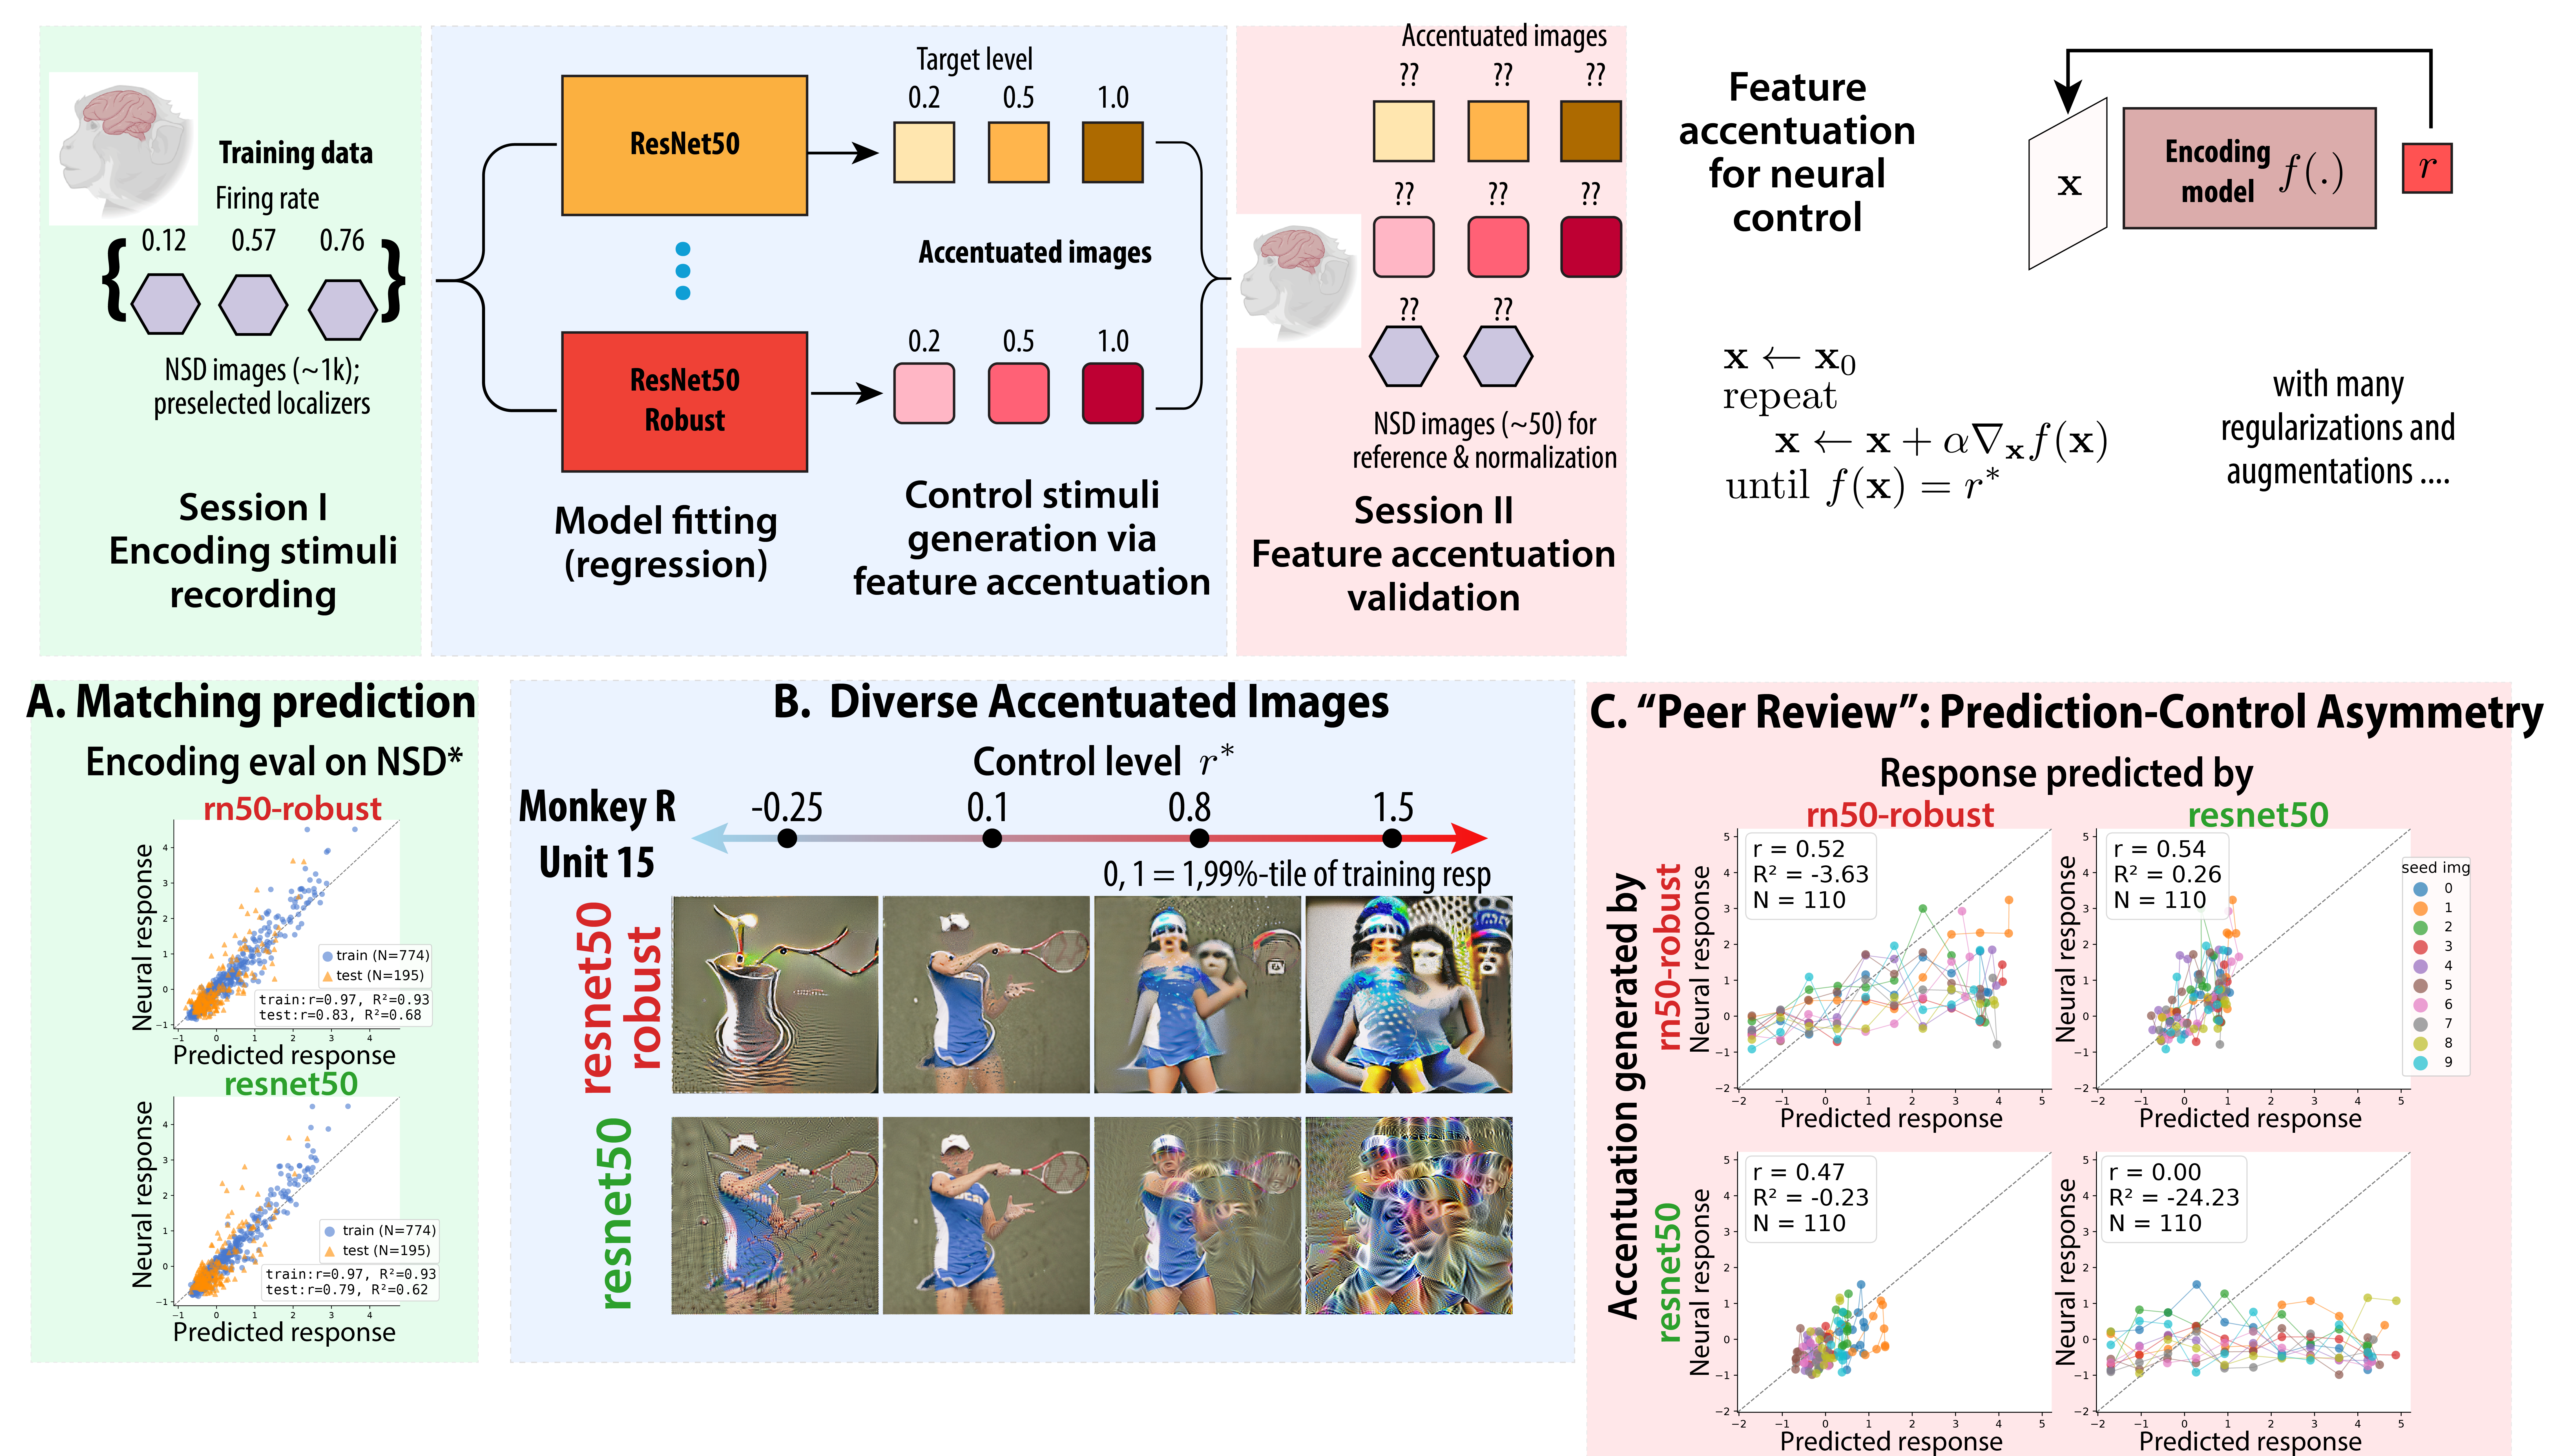
\includegraphics[width=\linewidth,height=0.27\textheight,keepaspectratio]{figures/Figure_NeuroCtrl_results.png}\\[2pt]
    \includegraphics[width=\linewidth,height=0.27\textheight,keepaspectratio]{figures/Figure_LinearToyModel.png}
    \caption{\textbf{The same three phenomena in neurons (top) and in a linear teacher--student model (bottom).}
    Top: closed-loop experiment of \citetPW. Encoding models are fit to responses to natural images, generate accentuated images for graded target responses, and are tested in a second session.
    \textbf{A}~Two models predict held-out natural-image responses equally well.
    \textbf{B}~Their accentuations from the same seed differ visibly, and only one modulates the neuron.
    \textbf{C}~Peer review: each model evaluated on the other's images. The weak controller tracks the strong controller's images but its own images barely modulate the neuron.
    Bottom: two linear students of a linear teacher (a disk-shaped weight on van~Hateren images), differing only along low-variance image directions, reproduce A--C exactly. Geometry inset: prediction sees weight error through the covariance ellipse; the accentuation path exposes the hidden Euclidean difference.}
    \label{fig:phenomena}
\end{figure}

Figure~\ref{fig:phenomena} (top) summarizes the closed-loop experiments of \citetPW: responses of visual cortical sites (V2--IT, 25 sites in 5 macaques) to $\sim$1000 natural images were recorded; ten deep-network encoding models were fit by ridge regression on network features with penalty and layer chosen by cross-validation; each model then synthesized, by gradient-based \emph{feature accentuation} \citep{hamblin2024feature}, images that drive its own prediction to eleven target levels from ten seed images; and the images were presented to the same sites. Three observations motivate this paper.

\paragraph{Similar prediction, divergent control.}
The trained models were tightly matched on held-out natural images, yet the slope and correlation between predicted and measured responses to their own accentuated images varied widely across models, with far larger spread than on natural images. Many models reached their requested \emph{predicted} response by adding texture and high-spatial-frequency structure that left the neuron largely unmoved.

\paragraph{Recognition without generation.}
Presenting model A's images to model B (``peer review'', Fig.~\ref{fig:phenomena}C) shows an asymmetry: a model whose own images fail to modulate the neuron still predicts the neuronal responses to a successful model's images with good correlation and better calibration than the generator itself. Models can recognize good control stimuli that they cannot produce.

\paragraph{Control tracks input-gradient structure.}
Across the 250 site--model pairs, control success is predicted by the spectral profile of the model's input gradient $\nabla_\x f$: models whose gradients concentrate power at low spatial frequencies, like natural images, control better. The two adversarially trained models are the strongest controllers, but the association persists without them.

The bottom row of Fig.~\ref{fig:phenomena} shows that a linear model reproduces all three observations once its weight error lies along low-variance directions of the image covariance. The remainder of the paper explains why finite-sample regression on noisy responses puts it there, why cross-validation does not remove it, and how the feature map decides how much of it reaches the pixel gradient.

\section{Three evaluations of one predictor}
\label{sec:setup}

\paragraph{Teacher and student.}
Inputs $\x\in\R^d$ are drawn from $\mathcal N(0,\Sigma)$ with $\Sigma=\sum_ks_k\uvec_k\uvec_k^\top$. A linear teacher with weight $\bstar=\sum_kb_k\uvec_k$ produces noisy responses $y=\x^\top\bstar+\sigma\epsilon$, and $S:={\bstar}^\top\Sigma\bstar$ is the natural response variance. The student is $f(\x)=\x^\top\bhat$, fitted from $n$ pairs $(X,\mathbf y)$; for feature-space students (Sec.~\ref{sec:feature}) $\bhat$ is the effective pixel weight $F^\top\hat w$, which is also the gradient $\nabla_\x f$.

\paragraph{Three distributions.}
Generalization evaluates $f$ on fresh natural inputs, $\x\sim\mathcal N(0,\Sigma)$. Accentuation evaluates $f$ on inputs it generates itself: gradient ascent from a seed $\x_0$ moves along $\nabla_\x f=\bhat$, so the idealized path is $\x=\x_0+\alpha\bhat$ with $\alpha$ set by the target level.\footnote{Deep-network accentuation adds preconditioning, augmentation and image priors \citep{hamblin2024feature}; App.~\ref{sec:app-evaluation-distributions} treats nonzero and multiple seeds.} In the main text $\x_0=0$ and the target range is variance-matched, $\Var[\alpha]({\bhat}^\top\bhat)^2=S$, so the student \emph{predicts} the natural response range along its path. Peer review evaluates $f$ on the path $\x_0+\alpha\bprime$ generated by another student $\bprime$. Writing $\Delta=\bhat-\bstar$ and applying the standard formulas for MSE, $R^2$ and the slope of true-on-predicted response to each distribution (App.~\ref{lem:mr-metrics}) gives Table~\ref{tab:evaluation-metrics}.

\begin{table}[t]
\centering\small
\begin{tabular}{@{}llccc@{}}
\toprule
Evaluation & Input covariance & MSE & $R^2$ & Slope \\
\midrule
Generalization & $\Sigma$ & $\Delta^\top\Sigma\Delta$ & $1-\Delta^\top\Sigma\Delta/S$ & ${\bhat}^\top\Sigma\bstar/{\bhat}^\top\Sigma\bhat$ \\
Accentuation & $\Var[\alpha]\,\bhat{\bhat}^\top$ & $S\,(1-N/D)^2$ & $1-(D/N-1)^2$ & $N/D$ \\
Peer review & $\Var[\alpha]\,\bprime{\bprime}^\top$ & $S\,({\bprime}^\top\Delta)^2/({\bprime}^\top\bprime)^2$ & $1-\big(\frac{{\bprime}^\top\bhat}{{\bprime}^\top\bstar}-1\big)^2$ & ${\bprime}^\top\bstar/{\bprime}^\top\bhat$ \\
\bottomrule
\end{tabular}
\caption{One fitted weight, three evaluation distributions. $N:={\bhat}^\top\bstar$, $D:={\bhat}^\top\bhat$. Pearson correlation is degenerate on a noiseless rank-one path and is omitted.}
\label{tab:evaluation-metrics}
\end{table}

\paragraph{Prediction is covariance-weighted, control is Euclidean.}
Generalization error is $\Delta^\top\Sigma\Delta$: a weight error along $\uvec_k$ costs $s_k$ times its squared length, so errors in low-variance directions are nearly invisible. Every accentuation metric, by contrast, is a function of the single scalar
\begin{equation}
z_{acc}:=\frac DN-1=\frac{{\bhat}^\top(\bhat-\bstar)}{{\bhat}^\top\bstar},
\qquad
\frac{E_{acc}}{S}=\Big(\frac{z}{1+z}\Big)^2,\quad R^2_{acc}=1-z^2,\quad \mathrm{slope}_{acc}=\frac{1}{1+z},
\label{eq:acc_metric_ND_depen}
\end{equation}
which weights $\Delta$ by $\bhat$ itself, with no covariance in sight. Geometrically (App.~\ref{prop:mr-iso-geometry}), the equal-$E_{gen}$ sets are ellipsoids around $\bstar$ elongated along low-variance axes, whereas the equal-$z_{acc}$ sets are Euclidean spheres with diameter from $0$ to $(1+z)\bstar$, and the equal-peer-error sets are hyperplanes normal to $\bprime$. A student can sit deep inside the prediction ellipsoid, far from the control sphere, and still lie on the peer hyperplane of a good generator: this is exactly the configuration of Fig.~\ref{fig:phenomena} (bottom), and it can be made arbitrarily extreme by adding weight along a direction with $s_k\to0$ (App.~\ref{ex:mr-dissociation}).

The remaining question is therefore not whether the dissociation is possible but when \emph{learning} produces it. Three ingredients are in play: finite-sample regression on noisy responses, the choice of regularization, and the feature map through which the gradient reaches the pixels. We take them in turn.

\section{Pixel-space ridge: noise, spectrum and the choice of regularization}
\label{sec:pixel}

Ridge regression in pixel space, $\bhat=\arg\min_\beta\frac1n\|X\beta-\mathbf y\|^2+\lambda\|\beta\|^2$, yields
\begin{equation}
\bhat=\underbrace{(\hat\Sigma+\lambda I)^{-1}\hat\Sigma\bstar}_{\text{shrunken signal}}
+\underbrace{\sigma(\hat\Sigma+\lambda I)^{-1}\tfrac1nX^\top\eta}_{\text{noise}},
\qquad \hat\Sigma=X^\top X/n .
\label{eq:ridge}
\end{equation}
Since ridge penalizes weight in low-variance directions, one might expect it to remove the hidden Euclidean error. We ask whether the error survives, and whether the cross-validated penalty removes it.

\begin{wrapfigure}{r}{0.5\linewidth}
    \vspace{-8pt}
    \centering
    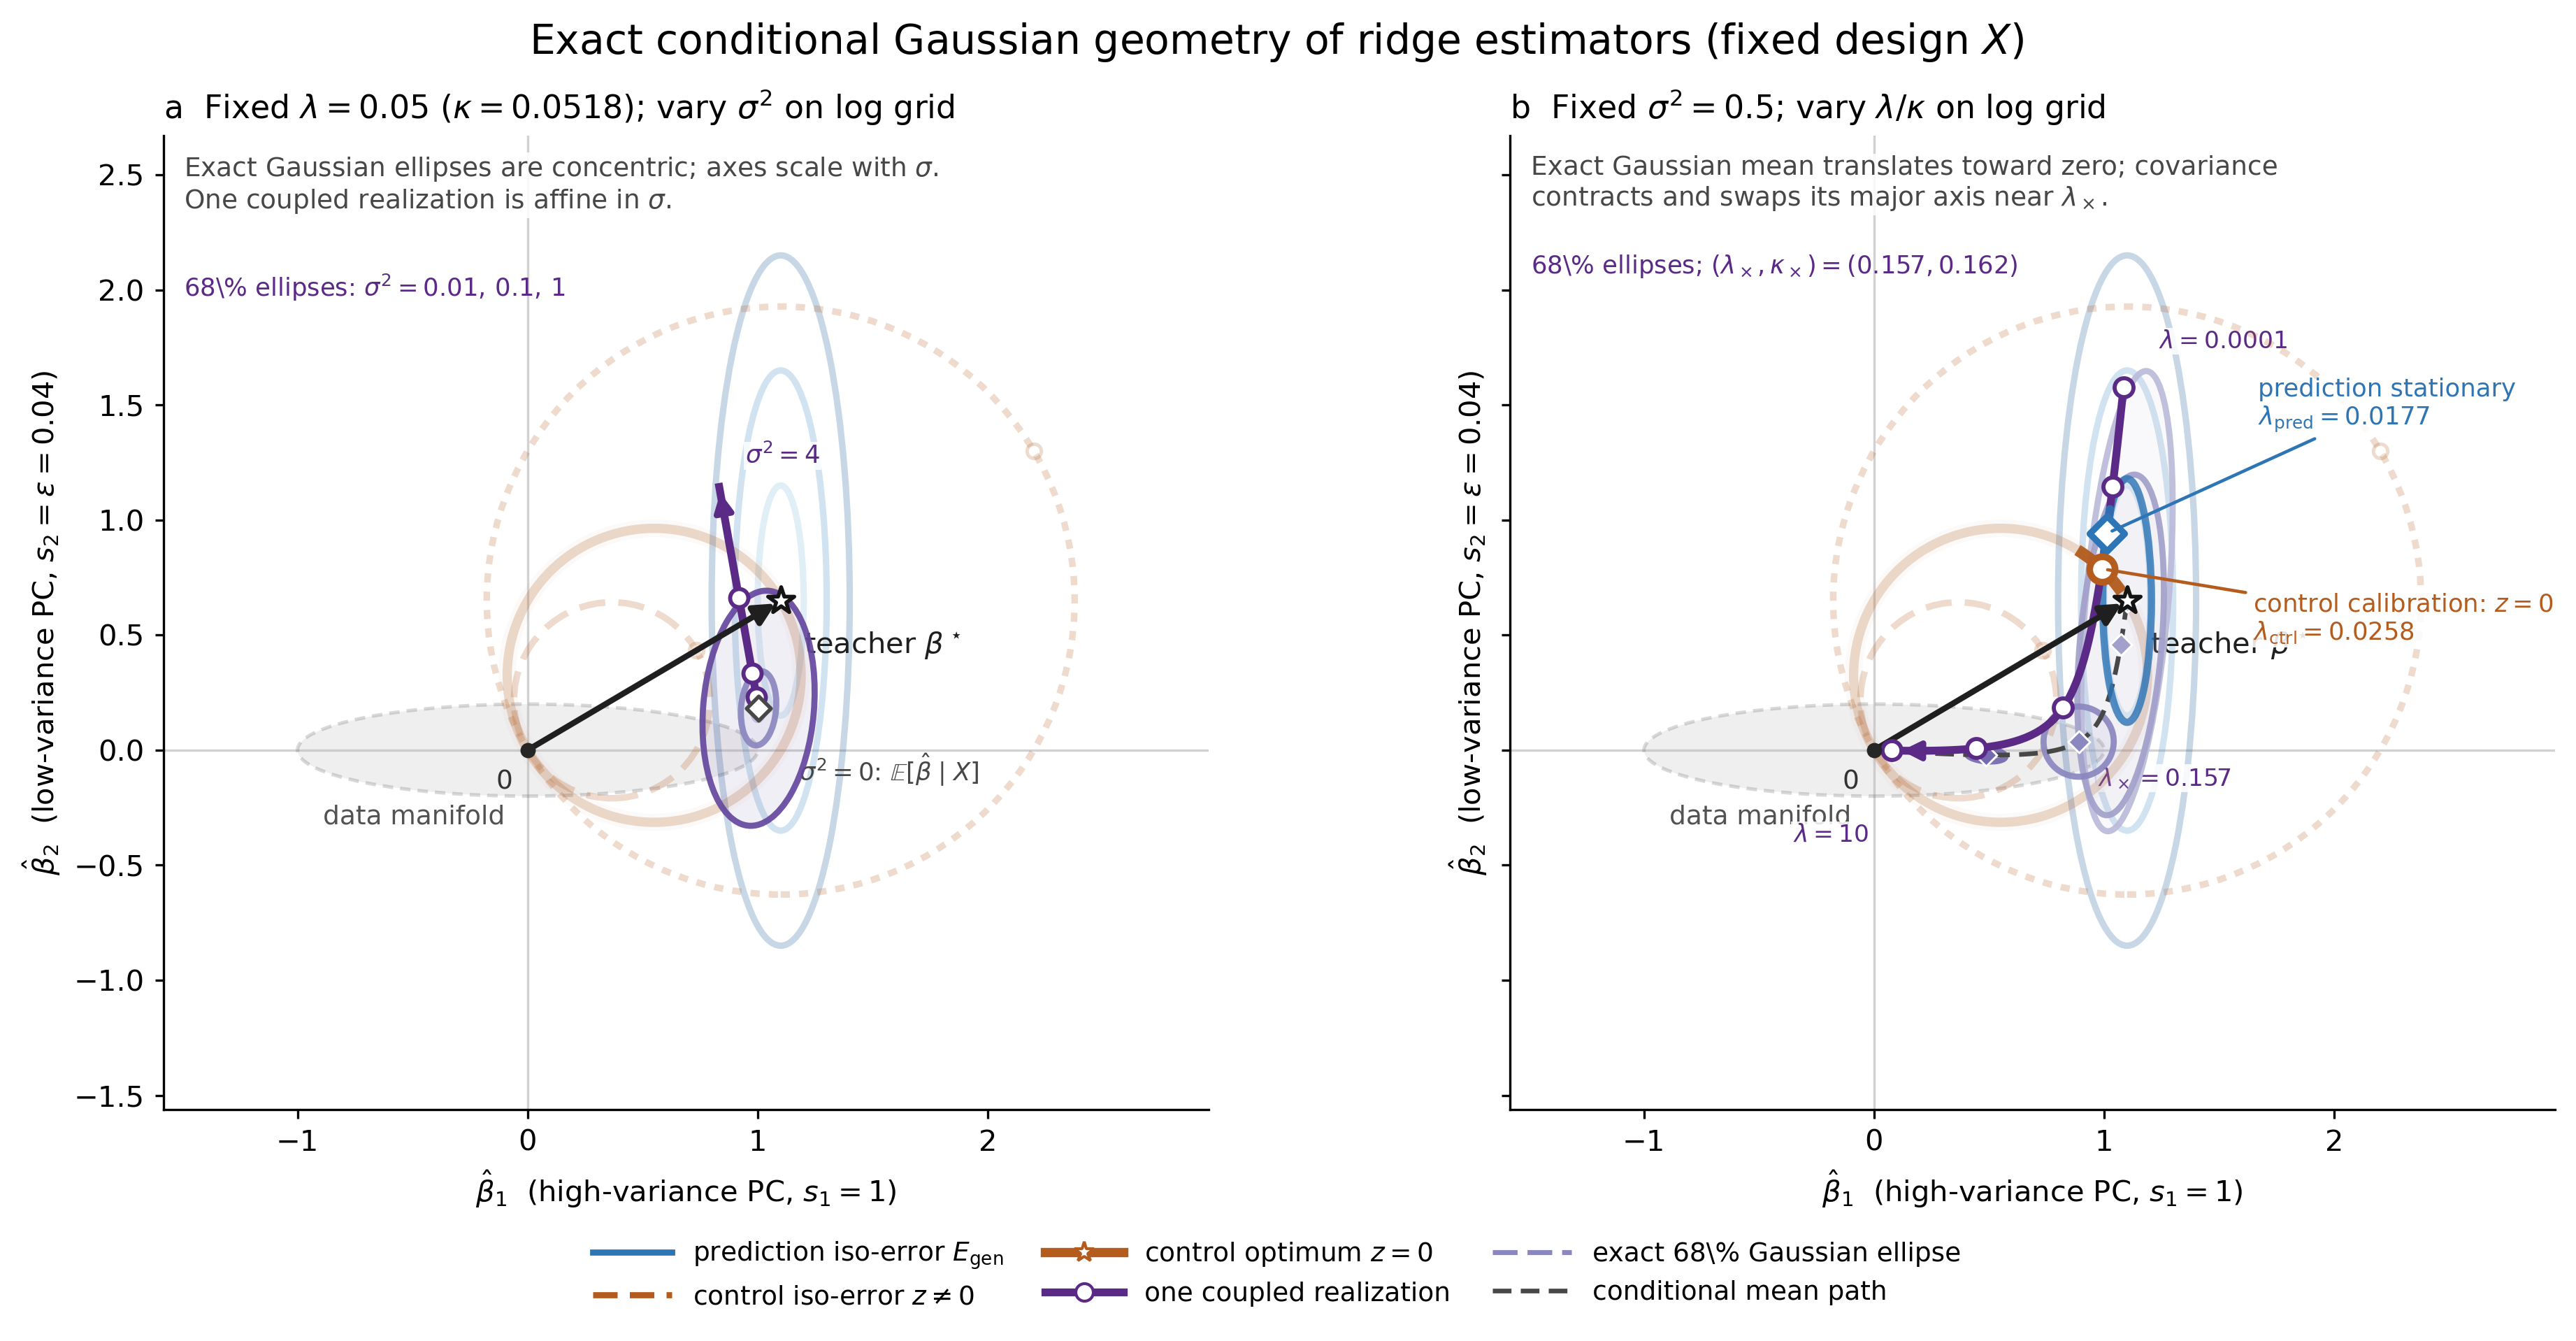
\includegraphics[width=\linewidth]{figures/draft_ridge_paths_iso_error_geometry.png}
    \caption{\textbf{Equal-error sets and the ridge path} in the plane of a high- and a low-variance PC. Prediction levels are ellipsoids around $\bstar$ (blue), control calibration is the sphere through $0$ and $\bstar$ (orange). The fitted weight is scattered around the ridge path (purple) with a spread elongated along the low-variance axis. Cross-validation picks the tangency of the path with an ellipsoid; control calibration is its crossing with the sphere. (Placeholder from the validation repository; to be polished.)}
    \label{fig:geometry}
    \vspace{-6pt}
\end{wrapfigure}
\paragraph{The ridge path through the two landscapes.}
The question has a geometric reading (Fig.~\ref{fig:geometry}). For a given training set, Eq.~\ref{eq:ridge} traces a path $\bhat(\lambda)$ in weight space from the least-squares or minimum-norm solution at $\lambda\to0$ to the origin at $\lambda\to\infty$. Response noise and the random design scatter the fitted weight in a cloud around this path, and the cloud is elongated along the low-variance directions of $\Sigma$, because those are the directions the data constrain least. Cross-validation selects the point of the path that is tangent to the smallest reachable prediction ellipsoid, whereas control calibration asks where the path crosses the sphere $D=N$; the two coincide only if the noise cloud has not pushed the path off the sphere in the directions the ellipsoid does not see. The deterministic equivalents below compute where the center of this cloud sits, how much Euclidean spread it carries, and hence the distance between the two points.


\paragraph{Toolkit.}
We use deterministic equivalents (DEs) in the proportional limit $d/n\to\gamma$ \citep{dobriban2018high,hastie2022surprises}. Finite-sample randomness enters through the effective penalty $\kappa(\lambda)$, the positive root of $\kappa-\lambda=\frac{\kappa}{n}\operatorname{Tr}[\Sigma(\Sigma+\kappa I)^{-1}]$, and the results are expressed through the teacher-weighted and unweighted spectral sums
\begin{equation}
B_{p,q}(\kappa)=\sum_k\frac{s_k^p}{(s_k+\kappa)^q}b_k^2,\qquad
\mathrm{df}_{p,q}(\kappa)=\sum_k\frac{s_k^p}{(s_k+\kappa)^q},\qquad \mathrm{df}_2:=\mathrm{df}_{2,2}.
\end{equation}
For the ratio $N/D$ we use the leading approximation $\mu_N/\mu_D$ obtained from the DEs of $N$ and $D$; its second-order and distributional refinements are in App.~\ref{sec:app-ratio-corrections} and matter only where the leading calibration error is already small.

\begin{prop}[Pixel ridge: prediction and control]\label{prop:pixel-de}
With $\kappa$, $B$ and $\mathrm{df}$ built from $\Sigma$,
\begin{equation}
E_{gen}\asymp E_{gen,DE}=\frac{n(\kappa^2B_{1,2}+\sigma^2)}{n-\mathrm{df}_2}-\sigma^2,
\qquad
\mu_N=B_{1,1},
\qquad
\mu_D=B_{2,2}+\frac{\mathrm{df}_{1,2}}{n}\big(E_{gen,DE}+\sigma^2\big).
\label{eq:pixel-de}
\end{equation}
\end{prop}
The three quantities are sums of the same per-eigenmode weight error (App.~\ref{prop:mr-per-pc}) with different weights: $E_{gen}$ weights mode $k$ by $s_k$, $D$ weights every mode equally. The last term of $\mu_D$ is the Euclidean energy of estimation noise, $\frac1n(E_{gen}+\sigma^2)$ per effective mode times $\mathrm{df}_{1,2}=\sum_ks_k/(s_k+\kappa)^2$, which counts modes near and below $\kappa$ heavily. It inflates the student's norm without helping it predict, so the student over-shoots along its own path: $z_{acc}>0$, slope $<1$. Ridge also shrinks the signal ($B_{2,2}<B_{1,1}$), which pulls in the opposite direction. Whether the two cancel is a question about $\lambda$. For natural images, whose spectrum decays as a power law over $10^4$ pixel modes, $\mathrm{df}_{1,2}$ counts thousands of weakly constrained high-spatial-frequency modes; the estimation noise that lands there is precisely the high-frequency texture of failed accentuations, and it costs almost nothing in $E_{gen}$.

\begin{prop}[Prediction-optimal and control-optimal penalties differ]\label{prop:pixel-tuning}
An interior minimizer of $E_{gen,DE}$ and a zero of the leading control error satisfy, respectively,
\begin{equation}
E_{gen,DE}+\sigma^2=n\kappa\frac{B_{2,3}}{\mathrm{df}_{2,3}}
\quad\text{(prediction)},\qquad
E_{gen,DE}+\sigma^2=n\kappa\frac{B_{1,2}}{\mathrm{df}_{1,2}}
\quad\text{(control)},
\label{eq:acc_optim_reg_cond1}
\end{equation}
so that at the prediction optimum the residual control error is
\begin{equation}
z^{(0)}_{acc,CV}=\frac{\kappa\,\mathrm{df}_{1,2}}{B_{1,1}}
\left(\frac{B_{2,3}}{\mathrm{df}_{2,3}}-\frac{B_{1,2}}{\mathrm{df}_{1,2}}\right)_{\kappa=\kappa^\star_{gen}} .
\label{eq:pixel-zacc-cv}
\end{equation}
\end{prop}
Both conditions equate the noisy prediction risk to $n\kappa$ times a teacher-weighted spectral average, but they average with different powers of $s_k/(s_k+\kappa)$. For isotropic data the two averages coincide and cross-validation calibrates control for free. For an anisotropic spectrum they differ whenever the teacher's energy is not uniformly distributed over modes, and the gap is multiplied by $\kappa\,\mathrm{df}_{1,2}$, i.e. by the number of modes near the regularization edge. In Fig.~\ref{fig:geometry}, Eq.~\ref{eq:pixel-zacc-cv} is the distance along the path between its tangency with the prediction ellipsoid and its crossing of the control sphere. This answers the question in the title for pixel regression: \emph{control is bad, despite prediction-optimal tuning, when the response is noisy, the spectrum is anisotropic, and many modes sit near $\kappa$}, which is the natural-image regime.

\begin{figure}[t]
    \centering
    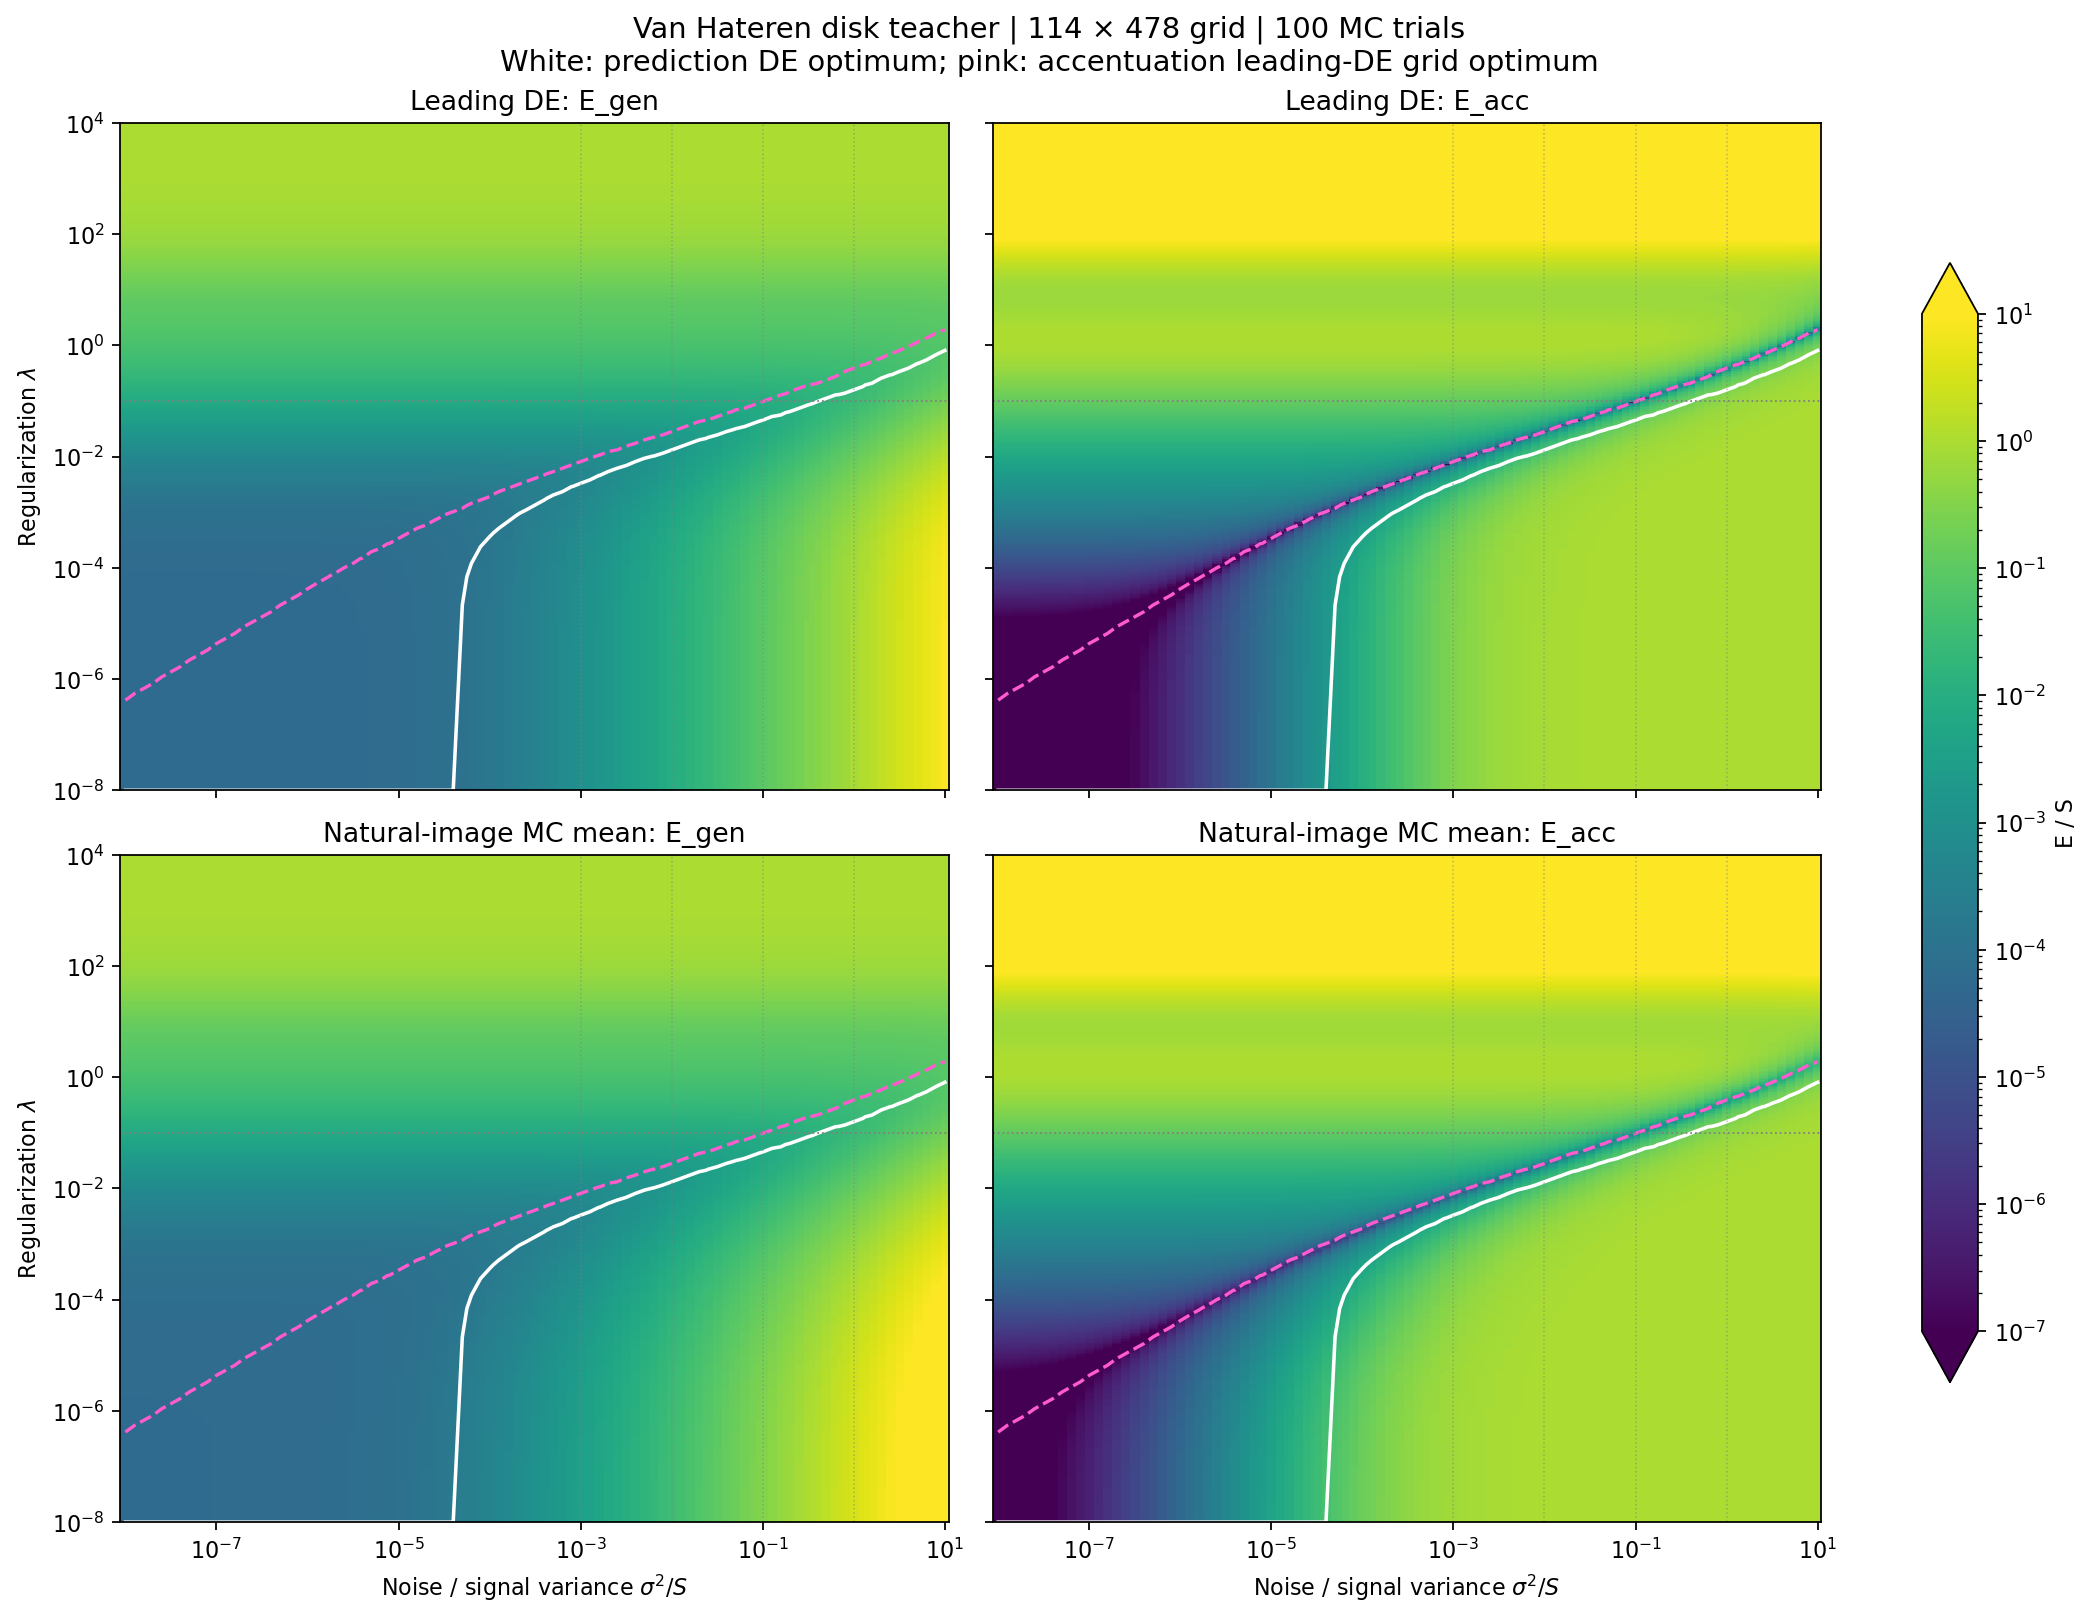
\includegraphics[width=0.48\linewidth,height=0.3\textheight,keepaspectratio]{figures/draft_landscape_error.png}\hfill
    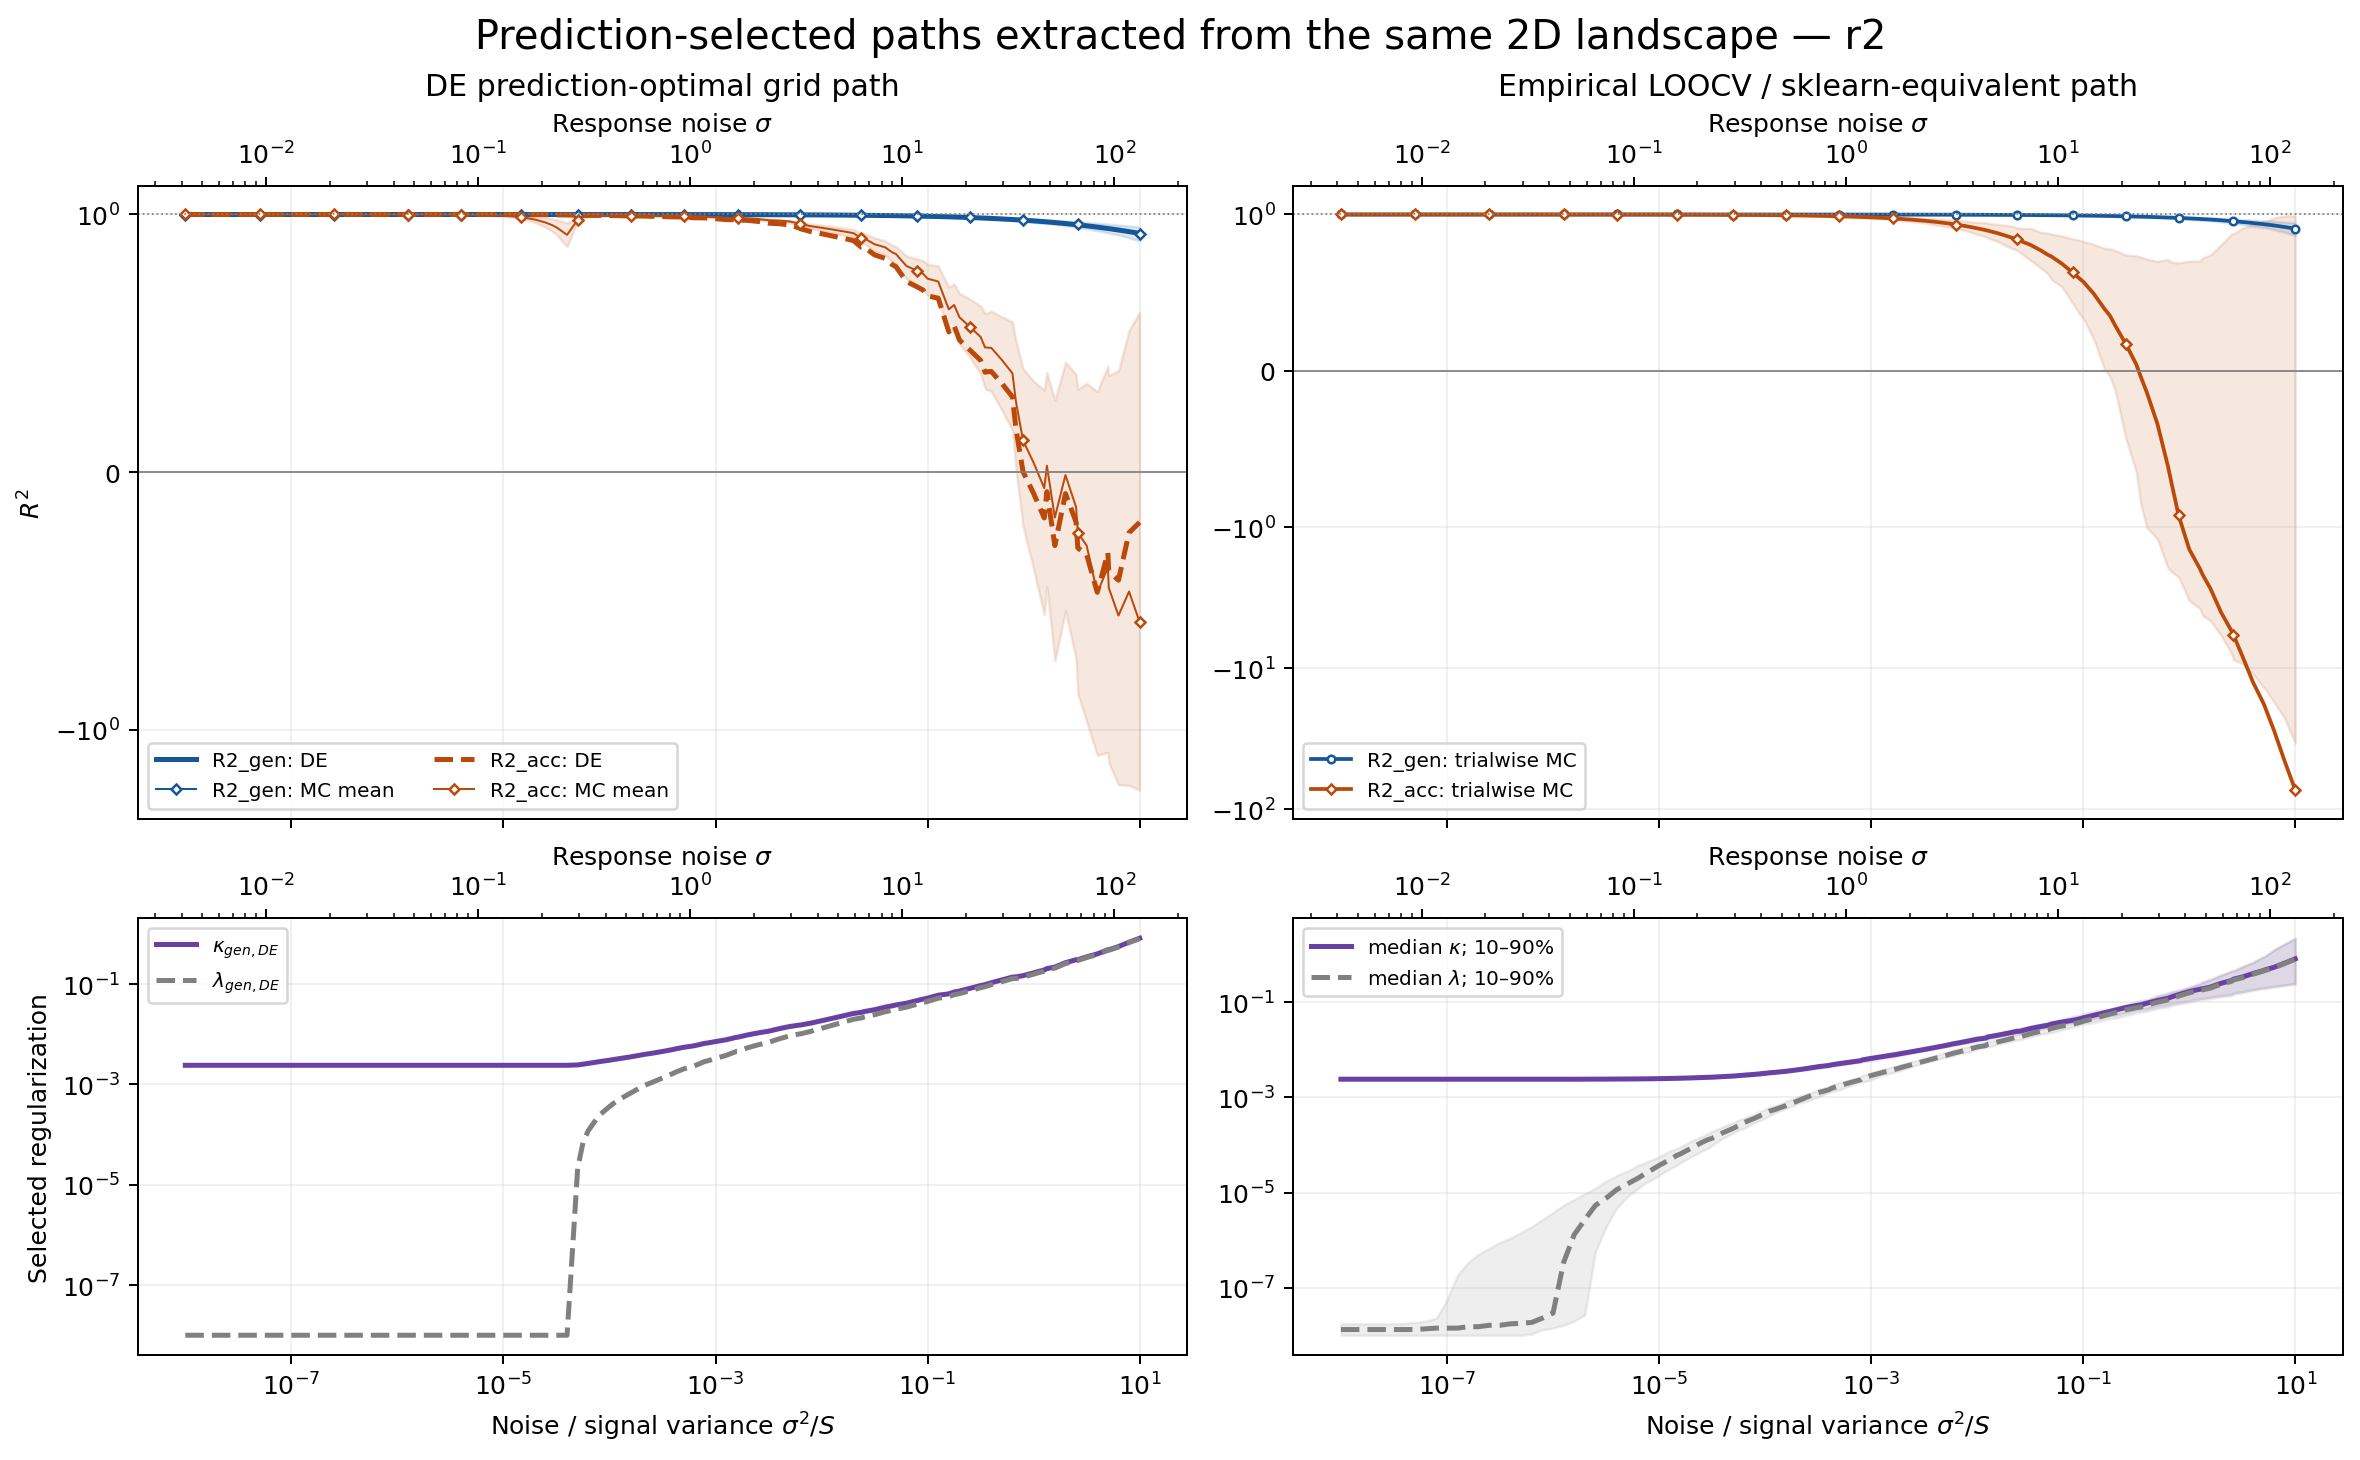
\includegraphics[width=0.5\linewidth,height=0.3\textheight,keepaspectratio]{figures/draft_slices_prediction_selected_r2.png}
    \caption{\textbf{Pixel ridge on van Hateren images ($d=10^4$, $n=10^3$, disk teacher).}
    \textbf{A}~Leading-DE control error $E_{acc}/S$ over noise $\sigma^2/S$ and penalty $\lambda$. The prediction-optimal path (white) and the control-calibrated path (pink) separate at all noise levels; Monte Carlo on real images (App.) reproduces the surface.
    \textbf{B}~Along the empirically cross-validated path, $R^2_{gen}$ stays above $0.9$ while $R^2_{acc}$ collapses once $\sigma^2/S\gtrsim0.1$; DE (lines) versus 100 natural-image trials (markers, 10--90\% band). Bottom: selected $\lambda$ and $\kappa$.}
    \label{fig:pixel}
\end{figure}

Figure~\ref{fig:pixel} confirms the picture on real natural-image regression. The DE surfaces track Monte Carlo over eight decades of noise; the prediction-optimal and control-calibrated penalties form two distinct ridges; and along the cross-validated path the student remains an excellent predictor while its accentuation $R^2$ becomes negative at moderate noise. 

\paragraph{Peer review: recognition without generation.}
Now evaluate $\bhat$ on the path of an independently fitted peer $\bprime$ at the same $\kappa$. The two noise realizations are uncorrelated, so the Euclidean noise term that inflates $D$ drops out of the cross products: ${\bhat}^\top\bprime\asymp B_{2,2}$ and ${\bstar}^\top\bprime\asymp B_{1,1}$, and the peer gain and score are
\begin{equation}
G_{peer}=\frac{{\bhat}^\top\bprime}{{\bstar}^\top\bprime}\asymp\frac{B_{2,2}}{B_{1,1}}\in(0,1],
\qquad
R^{2,(0)}_{peer}=1-\Big(1-\frac{B_{2,2}}{B_{1,1}}\Big)^2\in(0,1]
\label{eq:peer-de}
\end{equation}
(App.~\ref{prop:mr-peer}). Peer review measures only the shared shrinkage bias: at leading order it is never negative, degrades gracefully with noise, and is symmetric between the two fits. Self-evaluation instead carries the estimator's own Euclidean noise energy through Eq.~\ref{eq:pixel-de}, so $z_{acc}$ grows without bound with $\sigma^2/n$ and $R^2_{acc}$ becomes arbitrarily negative. A student can therefore track a peer's path while failing on its own, which is the linear form of Fig.~\ref{fig:phenomena}C. The asymmetry between a strong and a weak generator in the data arises when the two differ in noise energy, i.e. in their feature maps (Sec.~\ref{sec:feature}); and measured responses along a barely modulated path add trial noise that no evaluator can explain, which is why even the peer scores of a weak generator's images are poor.

\section{Feature-space ridge: the map decides what reaches the gradient}
\label{sec:feature}

Pixel regression explains why one student fails; it cannot explain why ten equally predictive backbones fail differently. We idealize a backbone as a fixed linear map $F\in\R^{p\times d}$, fit $\hat w$ by ridge on features $F\x$, and accentuate along the pixel gradient $\bhat=F^\top\hat w$. Let $C:=F\Sigma F^\top$ be the feature covariance and $G:=FF^\top$ the Euclidean feature Gram. The best realizable feature weight and its irreducible error are $w^\star=C^\dagger F\Sigma\bstar$ and $S_\perp=S-{w^\star}^\top Cw^\star$ (App.~\ref{lem:mr-feature-weights}).

\begin{prop}[Feature ridge: prediction and control]\label{prop:feature-de}\label{prop:linfeat_acc_ND}\label{prop:linfeat_gen_err}
With $\kappa$, $B^F$, $\mathrm{df}^F$ built from $(C,w^\star)$ and aspect ratio $p/n$,
\begin{equation}
E_{gen,DE}=\frac{n(\kappa^2B^F_{1,2}+S_\perp+\sigma^2)}{n-\mathrm{df}^F_2}-\sigma^2,\qquad
N_{DE}={\bstar}^\top\tilde\beta_\kappa,\qquad
D_{DE}=\|\tilde\beta_\kappa\|^2+\frac{E_{gen,DE}+\sigma^2}{n}\,T_F(\kappa),
\label{eq:feature-de}
\end{equation}
where $\tilde\beta_\kappa=F^\top(C+\kappa I)^{-1}F\Sigma\bstar$ is the mean pixel weight and
$T_F(\kappa):=\operatorname{Tr}[G(C+\kappa I)^{-2}C]$.
\end{prop}
Prediction sees the feature map only through $C$ and $F\Sigma\bstar$: the whole curve $E_{gen,DE}(\kappa)$, hence the cross-validated $\kappa$ and $R^2_{gen}$, is a function of $(C,F\Sigma\bstar,S,\sigma^2,n)$. Control additionally sees $G$, through $T_F$ and $\|\tilde\beta_\kappa\|$, and $F\bstar$, through $N_{DE}$ (Fig.~\ref{fig:feature}A). This is the statistical content of the dissociation: the prediction problem does not identify the control problem.

\begin{prop}[Prediction-preserving gauge]\label{prop:gauge}
For $\Sigma\succ0$ and any orthogonal $Q$ with $Q\Sigma^{1/2}\bstar=\Sigma^{1/2}\bstar$, the map $F\mapsto F\Sigma^{1/2}Q\Sigma^{-1/2}$ preserves $C$ and $F\Sigma\bstar$, hence the training law, $E_{gen,DE}(\kappa)$ and the DE cross-validated penalty, while changing $G$ and $F\bstar$ and therefore control.
\end{prop}
The gauge group is trivial for white data and grows with anisotropy. Rotating within it moves feature energy from high-variance to low-variance pixel directions at no cost to prediction (Fig.~\ref{fig:feature}B): along a continuous path, $E_{gen}$, $R^2_{gen}$ and the selected penalty are exactly constant, while $\operatorname{Tr}(FF^\top)$ grows by four orders of magnitude and $R^2_{acc}$ falls from near one to $-10^{8}$. Random draws from the family span this whole range (App.), so a population of equally predictive backbones with widely different control is the generic situation, not a construction.

\paragraph{What makes a map fragile.}
The factor $T_F$ is response-independent and has the spectral form (App.~\ref{prop:mr-fragility})
\begin{equation}
T_F(\kappa)=\sum_{k:s_k>0}\Big(\frac{s_k}{s_k+\kappa}\Big)^2\frac{\|g_k\|^2}{g_k^\top\Sigma g_k},
\qquad g_k:=F^\top v_k,
\label{eq:TF}
\end{equation}
with $(s_k,v_k)$ the eigenpairs of $C$. It averages, over the feature PCs that survive ridge shrinkage, the ratio between the Euclidean energy of the backpropagated PC gradient and its energy under the natural-image covariance. A map is fragile when its well-resolved feature directions backpropagate into low-variance, high-spatial-frequency pixel directions. This is the linear counterpart of the third observation of Sec.~\ref{sec:phenomena}, and it can be computed from the map and the image statistics alone.

\begin{center}
\fbox{\parbox{0.96\linewidth}{\small
\textbf{When is control fragile although prediction is fine?}
Holding the prediction error fixed, the leading control error (Eqs.~\ref{eq:pixel-de}, \ref{eq:pixel-zacc-cv}, \ref{eq:feature-de}) grows with three separable factors:
\textbf{(i) noise} $(E_{gen}+\sigma^2)/n$, the estimation-noise level, which is the only factor visible from held-out accuracy;
\textbf{(ii) spectrum} the mismatch between prediction-optimal and control-optimal penalties, Eq.~\ref{eq:pixel-zacc-cv}, which is zero for white data and grows with anisotropy and with teacher energy in low-variance modes;
\textbf{(iii) map} $T_F$, the ridge-weighted ratio of Euclidean to natural-covariance gradient energy, a property of the feature map alone.
Natural images make (ii) large for every model; the feature map decides (iii), and equally predictive maps can differ in it without bound.}}
\end{center}

\subsection{From the linear factor to a diagnostic for deep networks and neurons}
\label{sec:nonlinear}
For a nonlinear feature map $\phi$ with Jacobian $J_\phi(x)$ and natural-image feature covariance eigenpairs $(s_k,v_k)$, replacing $F$ by the local Jacobian in Eq.~\ref{eq:TF} gives
\begin{equation}
T_\phi(x,\kappa)=\sum_k\frac{s_k}{(s_k+\kappa)^2}\,\|J_\phi(x)^\top v_k\|^2,
\qquad
V_\phi:=\frac{E_{val}}{n}\,\E_x\big[T_\phi(x,\kappa)\big],
\label{eq:Tphi}
\end{equation}
where $J_\phi(x)^\top v_k=\nabla_x[v_k^\top\phi(x)]$ is the pixel gradient of feature PC $k$, obtainable by one backward pass per PC, and $V_\phi$ mirrors the variance term of Eq.~\ref{eq:feature-de}. For linear $\phi$ this is exact; for a network it is a diagnostic motivated by the theory, not a theorem, because the identity $s_k=g_k^\top\Sigma g_k$ that made $T_F$ a ratio of gradient energies no longer holds. Since an accentuation path travels far from the seed, we also evaluate smoothed versions in which the Jacobian is averaged, or the squared gradient is averaged, over a Gaussian neighborhood of the seed at pixel-noise scales from $0.5/255$ to $16/255$ (App.~\ref{sec:app-nonlinear-diagnostic}).

We computed these quantities for all 250 site--model pairs of the neuronal experiment, using each model's cross-validated ridge penalty and empirical feature spectrum to set $\kappa$, the ten experimental seed images for $\E_x$, and the held-out natural-image error of the control session for $E_{val}$. Because sites differ greatly in how controllable they are at all, we compare predictors after removing site means, so that each predictor is judged on ordering the ten models within a site (Fig.~\ref{fig:feature}C). Held-out prediction error carries essentially no information about which model will control better: its site-residual correlation with control slope is $0.03$ and with direct control error $-0.07$. The exact-local $V_\phi$ reaches $0.62$ with control slope and $0.44$ with control error across the nine trained models, and the trace $T_\phi$ alone does nearly as well, so the ordering comes from gradient geometry rather than from the prediction-error prefactor. Among the seven conventionally trained models the association is weaker but same-signed ($\approx0.2$ with slope), consistent with the two adversarially trained models being the strongest controllers and having by far the smallest $T_\phi$. Neighborhood-smoothed versions preserve or slightly improve the ordering. These are descriptive associations with repeated models within sites, not independent-sample tests, and they concern model ordering rather than absolute control error, for which the teacher-dependent terms of Eq.~\ref{eq:feature-de} would also be needed.

\begin{figure}[t]
    \centering
    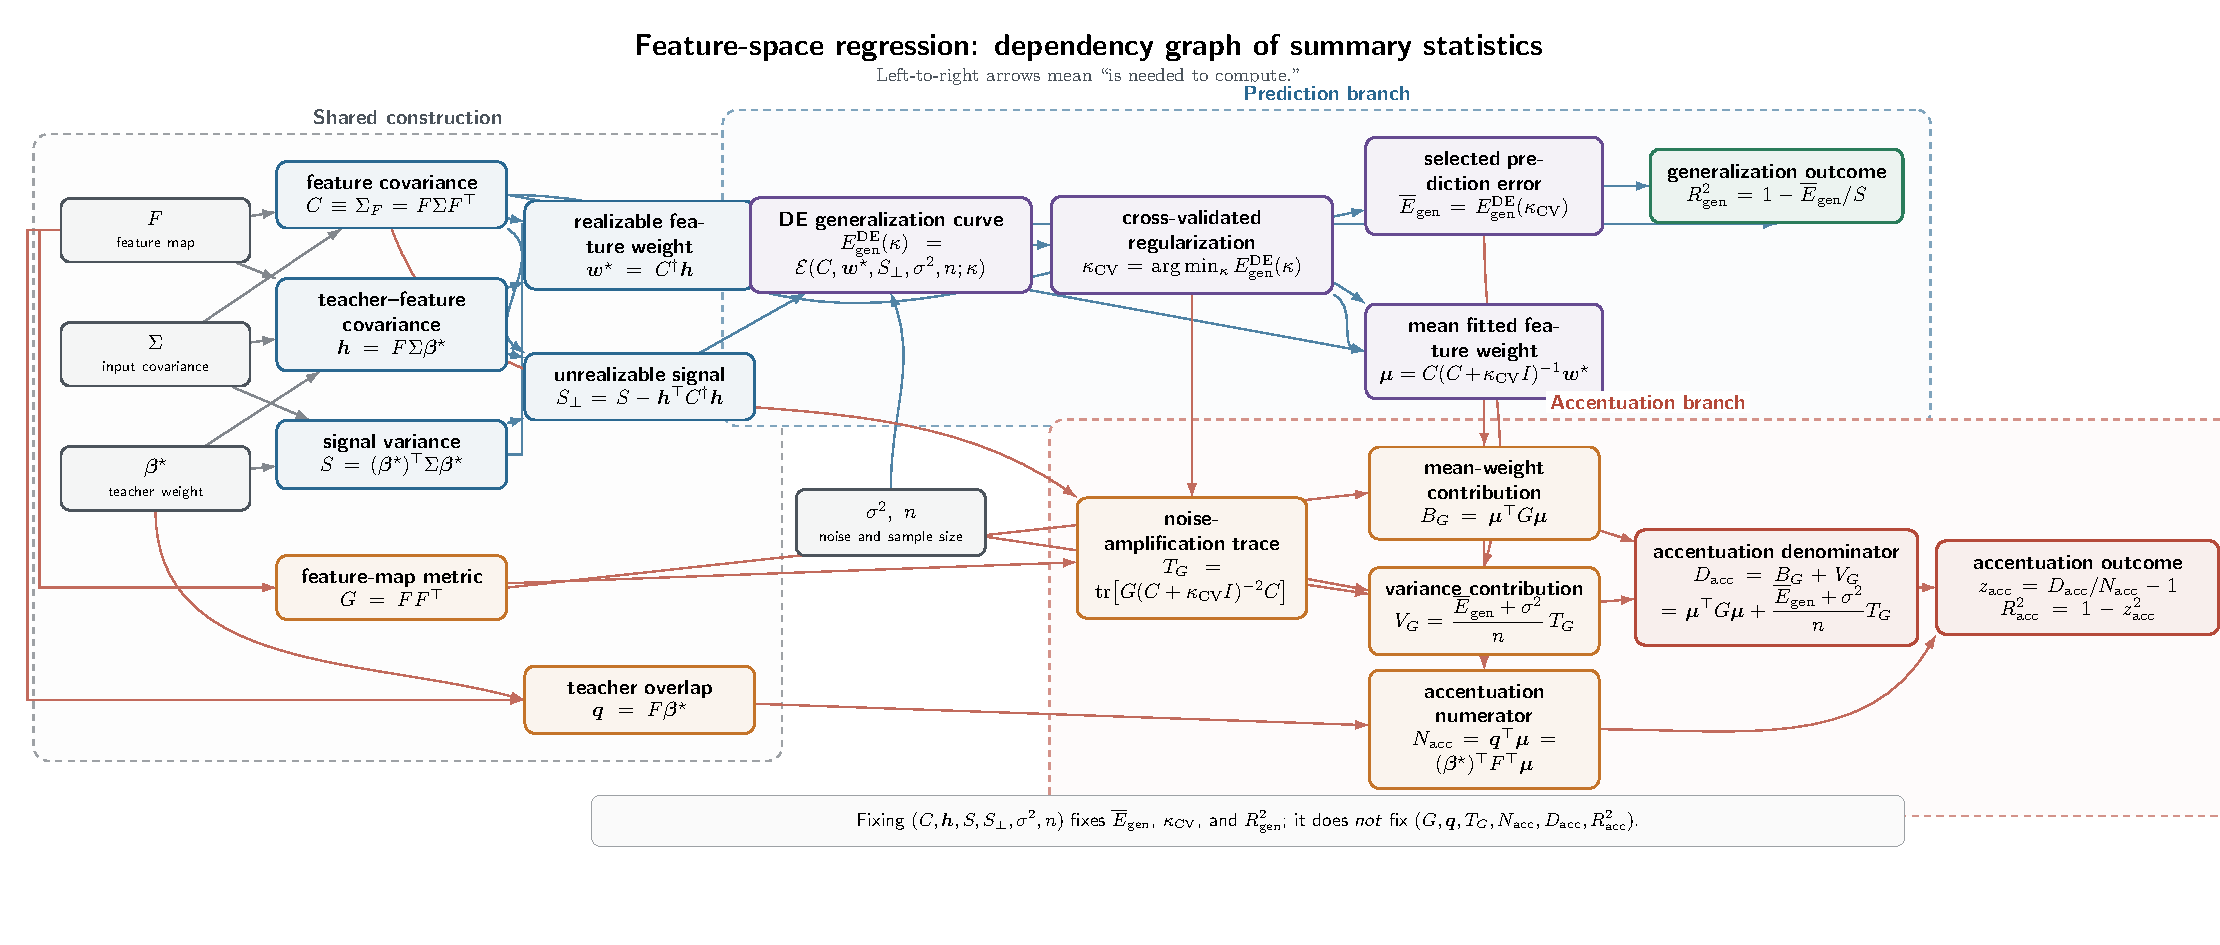
\includegraphics[width=0.55\linewidth,height=0.22\textheight,keepaspectratio]{figures/feature_summary_statistics_flow.pdf}\hfill
    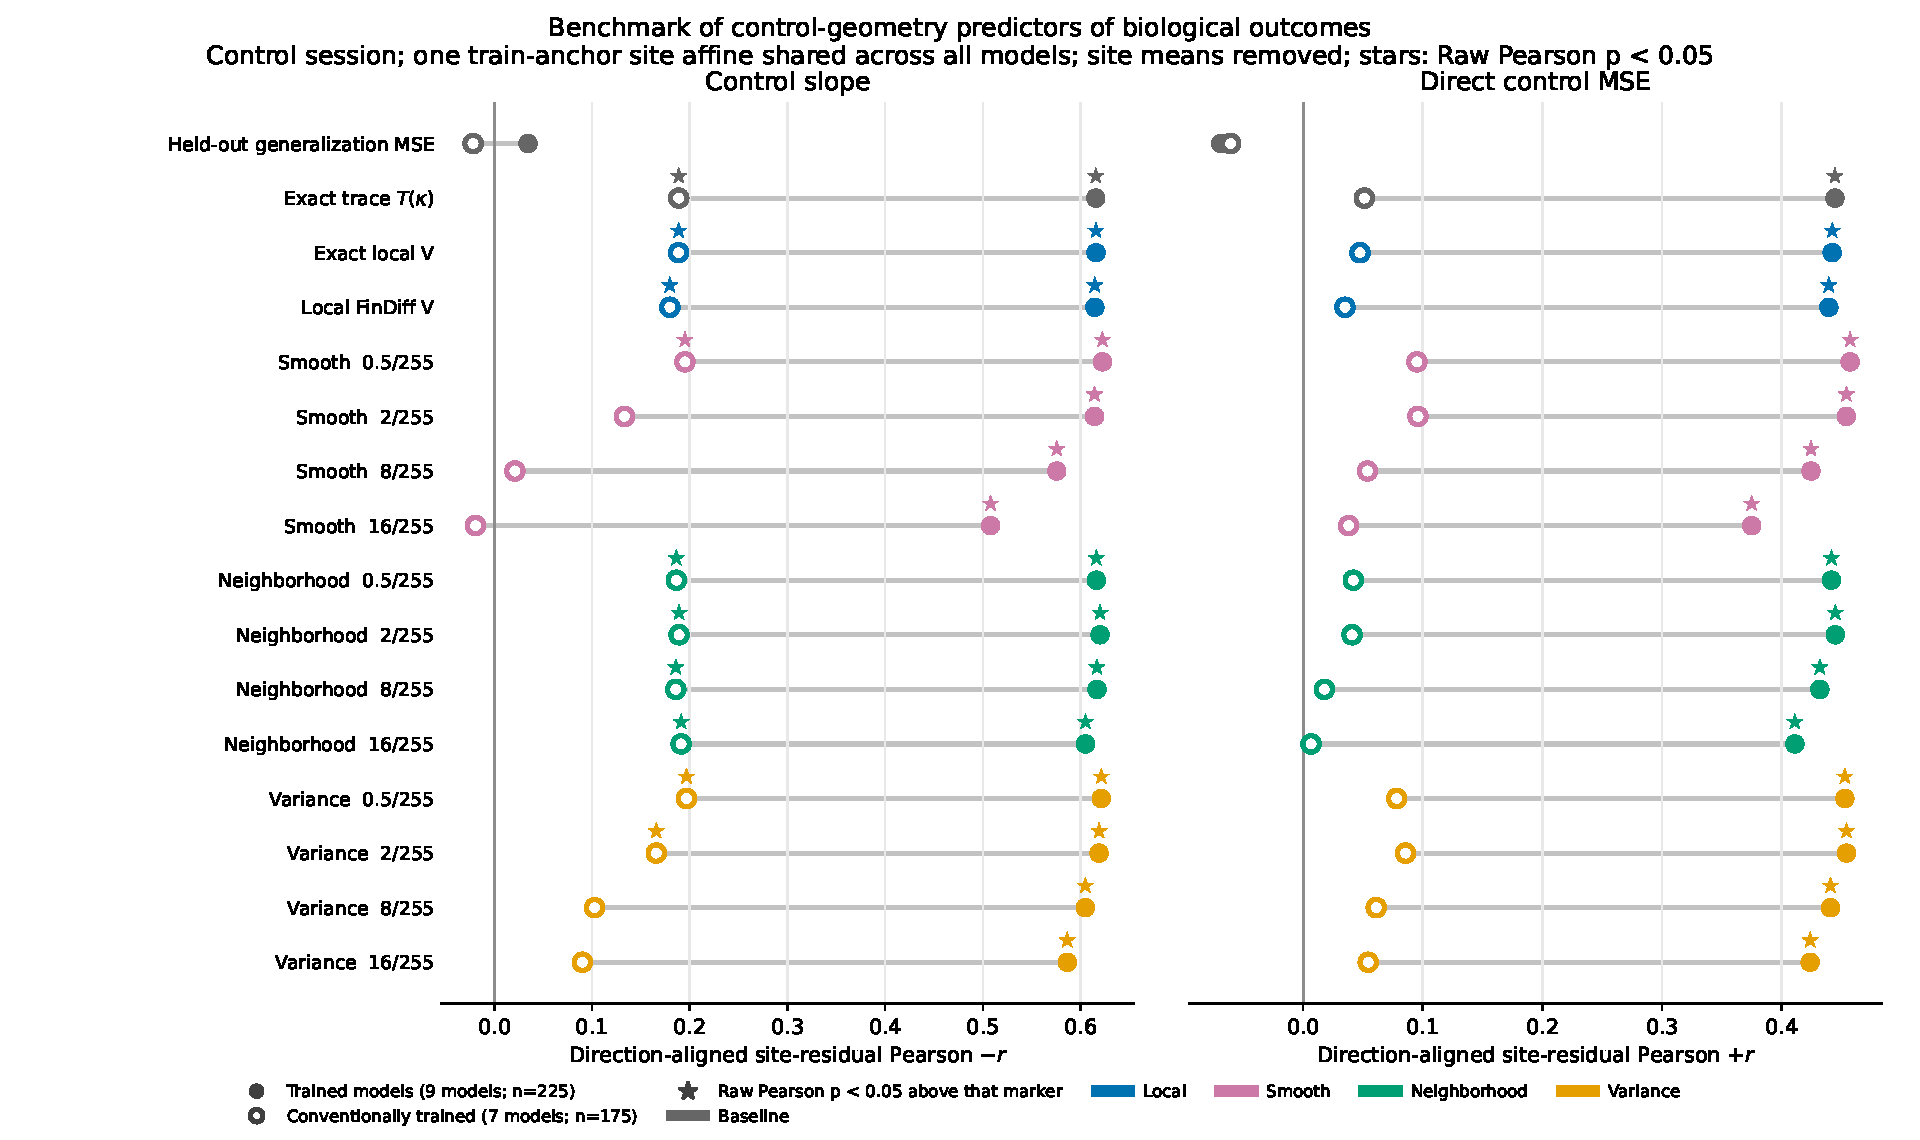
\includegraphics[width=0.44\linewidth,height=0.22\textheight,keepaspectratio]{figures/nonlinear_control_biological_validation.pdf}\\[2pt]
    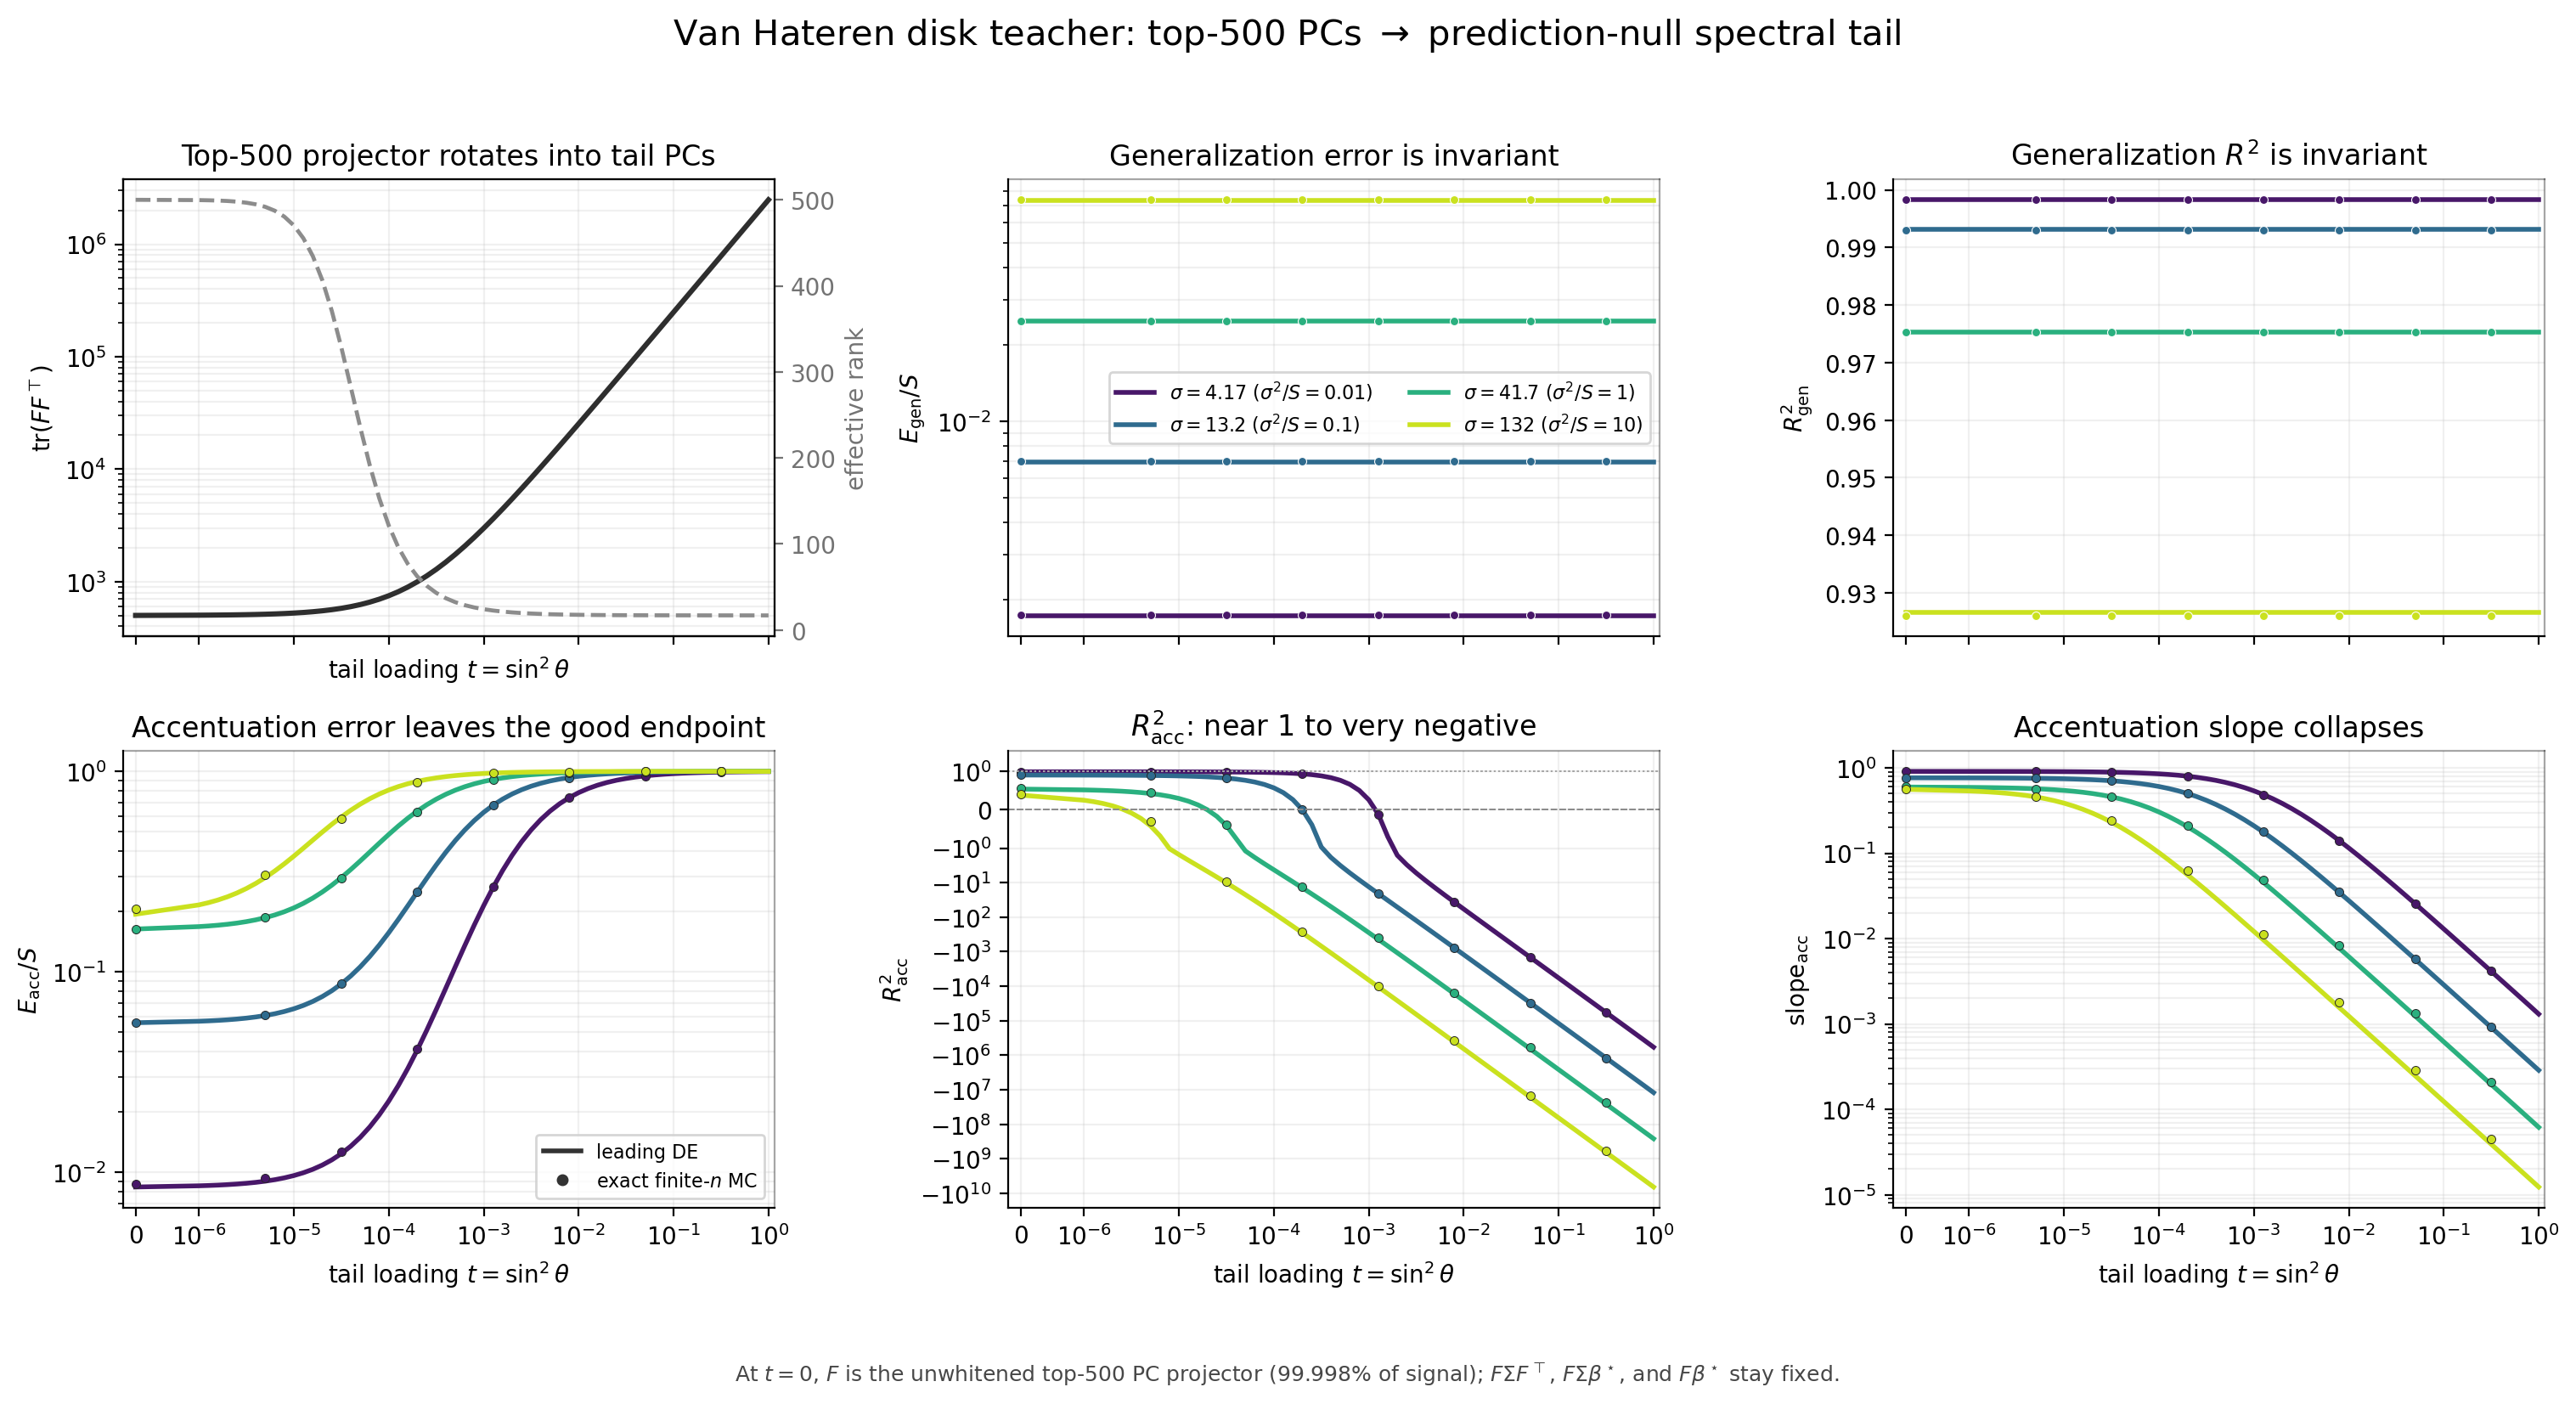
\includegraphics[width=\linewidth,height=0.2\textheight,keepaspectratio]{figures/VanHateren_Top500PC_prediction_null_feature_rotation.png}
    \caption{\textbf{Feature geometry decides control.}
    \textbf{A}~Dependency graph: $(C,F\Sigma\bstar,S,\sigma^2,n)$ fix generalization and the cross-validated penalty; control additionally needs $G=FF^\top$ and $F\bstar$ (draft: to be simplified to $\sim$8 boxes).
    \textbf{B}~Rotating a top-500-PC projector of van Hateren images into the prediction-null spectral tail: $E_{gen}$ and $R^2_{gen}$ are invariant while $R^2_{acc}$ and the slope collapse; DE (lines) matches finite-$n$ Monte Carlo (markers). (Draft: keep 3 of 6 panels.)
    \textbf{C}~Neuronal data: site-demeaned association of each candidate predictor with biological control slope (left) and control error (right) across nine trained (filled) and seven conventionally trained (open) models. Held-out error carries no model-order information; the exact trace, $V_\phi$ and its neighborhood versions do. (Draft: keep 5 rows.)}
    \label{fig:feature}\label{fig:nonlinear-biological-validation}
\end{figure}

\section{Discussion}
\label{sec:discussion}
A single mechanism accounts for the three neuronal phenomena: prediction measures weight error in the covariance metric, control measures it along the model's own gradient. In the linear theory the control error at fixed prediction error is governed by the three factors of the box in Sec.~\ref{sec:feature}: noise, spectrum, and map, of which only the first is visible from held-out accuracy. The practical implication is that selecting encoding models or penalties by held-out prediction cannot certify gradient-based control; validation must constrain the gradient, for instance through $T_\phi$, or test generated stimuli directly. The high-frequency artifacts of failed accentuations are not a cosmetic defect but the expected signature of low-variance directions that natural images never constrained.

\paragraph{Limitations.}
The theory assumes Gaussian inputs, a linear teacher, a fixed linear feature map and a one-dimensional accentuation path from a centered seed; the leading DEs predict typical fits and the location of the control optimum but not the fluctuation-dominated error at that optimum (App.~\ref{sec:app-ratio-corrections}). The nonlinear diagnostic is not a theorem, and its biological validation is descriptive. Extending the deterministic equivalents to learned nonlinear features and to curved accentuation trajectories is the natural next step.

% ---------------------------------------------------------------------------
% Compact narrative draft of the main text (Sections 1-6).
% Companion: theory_appendix_main_results.tex holds every statement in full,
% in derivation order.  Here propositions are stated only where they carry the
% story; everything else is a pointer.
%
% Figure plan (3 figures):
%   Fig 1  neuronal results (top row) + linear recapitulation (bottom row)
%   Fig 2  pixel ridge: landscape + CV path
%   Fig 3  feature ridge: dependency graph + null rotation + biological validation
%   wrapfig  iso-error geometry + ridge path (Sec 3)
% ---------------------------------------------------------------------------

\begin{abstract}
Deep neural networks are increasingly used both as encoding models of visual cortex and as controllers that synthesize images to drive neural responses toward desired states. Recent \textit{in vivo} experiments reveal a striking dissociation: models with nearly identical held-out accuracy can generate qualitatively different stimuli and differ sharply in control, and these differences track input-gradient structure better than predictive accuracy. We develop a geometric and analytical account of this phenomenon in a linear teacher–student model. The key is that control creates a self-generated distribution shift. Natural-image generalization, self-accentuation, and peer review evaluate the same fitted predictor under three different input distributions; correspondingly, their equal-error sets in weight space are ellipsoids, spheres, and hyperplanes.
% Generalization weights estimation error by the data covariance, whereas self-accentuation exposes it along the model’s own fitted direction in Euclidean geometry.
Using deterministic equivalents for ridge regression, we show that prediction-optimal and control-optimal regularization satisfy different spectral conditions, so cross-validation can leave large control error when responses are noisy and inputs are anisotropic. Extending the analysis to fixed linear feature maps, we construct a prediction-preserving gauge family with identical generalization and cross-validated regularization but arbitrarily different control. Control is most fragile when feature directions that survive regularization backpropagate into low-variance, high-spatial-frequency image directions. The resulting gradient-geometry factor extends to nonlinear networks as a Jacobian-based diagnostic and predicts across-model variation in \textit{in vivo} control better than held-out prediction error. Thus predictive accuracy alone cannot certify control; the model’s gradient geometry or generated stimuli must also be evaluated.
% Deep neural networks are increasingly used both as encoding models of visual cortex and as controllers that synthesize images to drive neural responses toward desired states. Recent \textit{in vivo} experiments show that, models with similar held-out accuracy in predicting visual-neuron responses can differ sharply in the features they rely on and in their ability to generate stimuli to control those neurons. Moreover, the control success is more associated by the structure of a model's input gradient than its predictive accuracy.
% We develop a geometric and analytical account of this prediction--control dissociation using a linear teacher--student model.
% Classic generalization evaluates a fitted predictor on the natural-image distribution; model-based control evaluates it on a path along its own fitted direction. Such difference in evaluation distribution leads to different iso-error geometry in the weight space.
% %feature accentuation evaluates it on a distribution generated along its own fitted direction.
% % This change of distribution gives control error, $R^2$, and response slope a different dependence on estimation error than test loss: prediction weights error by the data covariance, control counts it in Euclidean geometry.
% Using deterministic equivalents for ridge regression we show that prediction-optimal and control-optimal regularization obey different spectral conditions, so cross-validation can leave large control error under noisy, anisotropic data. Extending the analysis to fixed linear feature maps, prediction depends only on the feature covariance and its alignment with the teacher, whereas control additionally depends on the map's input-gradient geometry. We construct a gauge family of feature maps with identical generalization performance, but arbitrarily different control. Control is most fragile when the feature directions that survive regularization backpropagate into low-variance, high-spatial-frequency image directions. The resulting gradient-geometry factor extends to nonlinear networks as a diagnostic and predicts the variation of \textit{in vivo} control capability of models better than held-out prediction accuracy.
\end{abstract}

% suggested new abstract content - maybe something in here is useful
% Deep neural networks are increasingly treated as models of primate visual processing and used to predict neural responses in visual cortex. These mappings from image space to brain activity, known as encoding models, can also be used to attempt neural control, by synthesizing images that are predicted to drive neural firing into a chosen state. Surprisingly, recent large-scale in vivo experiments found that many leading models with nearly identical held-out predictive accuracy over natural images differ substantially in their capacity for neural control. Here we develop a geometric and analytical account of this prediction-control dissociation. Using a linear model of a neuron whose true preferences are known, we make two key observations. First, prediction and control evaluate the same model on different inputs. Natural image prediction relies on images that vary widely along some dimensions and hardly at all along others, with errors along rarely explored directions not reflected in generalization scores.  Controller stimuli instead exaggerate the hypothesized directions of neural sensitivity, directly targeting the underexplored directions and exposing exactly those errors. Second, the ridge regularization best for prediction generally differs from the one best for control, so standard cross-validation can leave large control errors, especially when data are noisy. Extending the theory to models built on fixed features, we show that equally predictive models can differ arbitrarily in control, depending on how much their input gradients rely on these neglected directions. Measuring this reliance yields a diagnostic that can be computed before any control experiment. On the neural dataset that motivated this study, this diagnostic predicts which models will best control each neural site, while natural image predictivity carries almost no information. These results imply that models selected for natural-image predictivity, as in most current benchmarks, may not support effective control, and that future evaluations should test a model's gradients or generated stimuli directly.


\section{Introduction}
A good predictive model of a neuron can, in principle, be used as a \textit{model-based} controller: if $f(\x)$ predicts the response of a neuron to an image $\x$, one can synthesize images that drive $f$ to a target level and present them to the subject to modulate neuronal state.
Aside from model-free generative search \citep{ponce2019evolvingImages,xiao2020xdream}, model-based control of visual neurons has been successfully pursued across species \citep{bashivan2019neuralPopulationControl,walker2019inceptionLoops}. Recently, \citetPW scaled this paradigm into a benchmark of many deep-network encoding models and uncovered three puzzles: Encoding models that are nearly indistinguishable on predicting held-out natural images generate visibly different stimuli and differ several-fold in how well those stimuli modulate the neuron \textit{in vivo}; models that fail to control can still recognize the successful stimuli of other models; and the best predictor of control success is not accuracy but the spectral structure of the model's input gradient.

% We argue that none of this requires nonlinearity, depth or biology.
We argue that these phenomena arise already in linear models, from a single fact: \emph{control evaluates a model on a distribution the model generates itself}. Held-out prediction measures weight error in the metric of the data covariance $\Sigma$, which suppresses low-variance directions; accentuation moves along the fitted weight itself and therefore measures the same error in Euclidean geometry, where nothing is suppressed. For natural images, whose covariance spectrum decays over many orders of magnitude, this is the difference between not seeing an error and being dominated by it.

Our contributions are:
\textbf{(I)} a formulation of generalization, self-accentuation and peer review as evaluations of one predictor under three input distributions, with their equal-error sets (ellipsoid, sphere, hyperplane) exposing the dissociation geometrically (Sec.~\ref{sec:setup});
\textbf{(ii)} deterministic equivalents for pixel-space ridge regression showing that prediction-optimal and control-optimal penalties satisfy different spectral conditions, so cross-validation in anisotropic data and teacher leaves a computable residual control error (Sec.~\ref{sec:pixel});
\textbf{(iii)} for ridge regression on a fixed linear feature map, a separation of the summary statistics that determine prediction from those that determine control, and a gauge family of feature maps with identical generalization but arbitrarily different control (Sec.~\ref{sec:feature});
\textbf{(iv)} a response-independent gradient-geometry factor $T_F$ that identifies fragile feature maps, extends to nonlinear networks as a diagnostic, and recovers model ordering in the neuronal control data.
All statements are proved in the appendix, where we also restates every result in derivation order (App.~\ref{sec:app-main-results}); numerical validation against Monte Carlo accompanies each section. %and natural-image regression

% \paragraph{Related work.}
% High-dimensional ridge regression under anisotropic covariance is classical \citep{dobriban2018high,hastie2022surprises}, and deterministic equivalents for its risk are standard \citep{bai2010spectral,couillet2011random}; we use this toolkit but change the evaluation distribution from the training law to a model-generated path. Optimizing inputs against a fitted model is the setting of feature visualization and accentuation \citep{olah2017feature,hamblin2024feature}, adversarial examples and performative prediction; our contribution is a solvable model in which the resulting distribution shift is computed rather than assumed. %Model-based closed-loop neuroscience \citepPW\ supplies the phenomena.
\paragraph{Related work.}
Encoding models built on deep networks now predict cortical responses so similarly that benchmarks no longer rank them \citep{yamins2014performanceOptimized,guclu2015deepGradientComplexity,cadena2019deepConvolutionalV1,schrimpf2018brainscore,conwell2024inductiveBiases}. Read one way this is convergence \citep{huh2024platonicRepresentationHypothesis,kapoor2026convergentLearning}; read another it is a weak test, answered by constraining the mapping \citep{prince2024sparsePositiveAlignment} or by seeking stimuli that split models apart \citep{golan2020controversialStimuli,feather2023modelMetamers,rajalingham2018large,geirhos2019imagenetTextureBias}. Closed-loop control is one limit of that strategy: the model writes the stimulus and the neuron grades it \citep{ponce2019evolvingImages,xiao2020xdream,bashivan2019neuralPopulationControl,walker2019inceptionLoops,prince2026parametric}. Optimizing an input against a fitted model likewise underlies feature visualization \citep{olah2017feature,hamblin2024feature,fel2023magnitudeConstrainedOptimization} and adversarial attack \citep{nguyen2015deepNeuralFooled,goodfellow2015explainingAdversarial,madry2018towardsResistant}, where robustness has been tied to alignment \citep{guo2022adversariallyTrainedNeuralRepresentations,dapello2020simulatingV1,taori2020measuring}.
In each case the test distribution is created by the model under test, which we make analytical.
Classic theory characterizes ridge risk under anisotropic covariance and signal--spectrum alignment \citep{dobriban2018high,hastie2022surprises,mei2022generalization,mel2021highDimensionalRegression}, as well as generalization and optimal regularization under an externally specified train--test distribution shift \citep{canatar2021outOfDistribution,tripuraneni2021covariateShift,patil2024optimalOODRidge}. We instead study a self-generated shift: the test distribution is supported on an optimization path created by the fitted predictor itself.
%  carrying theory of ridge risk under anisotropic covariance \citep{dobriban2018high,hastie2022surprises,mei2022generalization,bai2010spectral,couillet2011random} off the training law  and onto the model's own path.

\section{Prediction and control dissociate in neurons and in linear regression}
\label{sec:phenomena}

\begin{figure}[t]
    \centering
    \vspace{-14pt}
    % 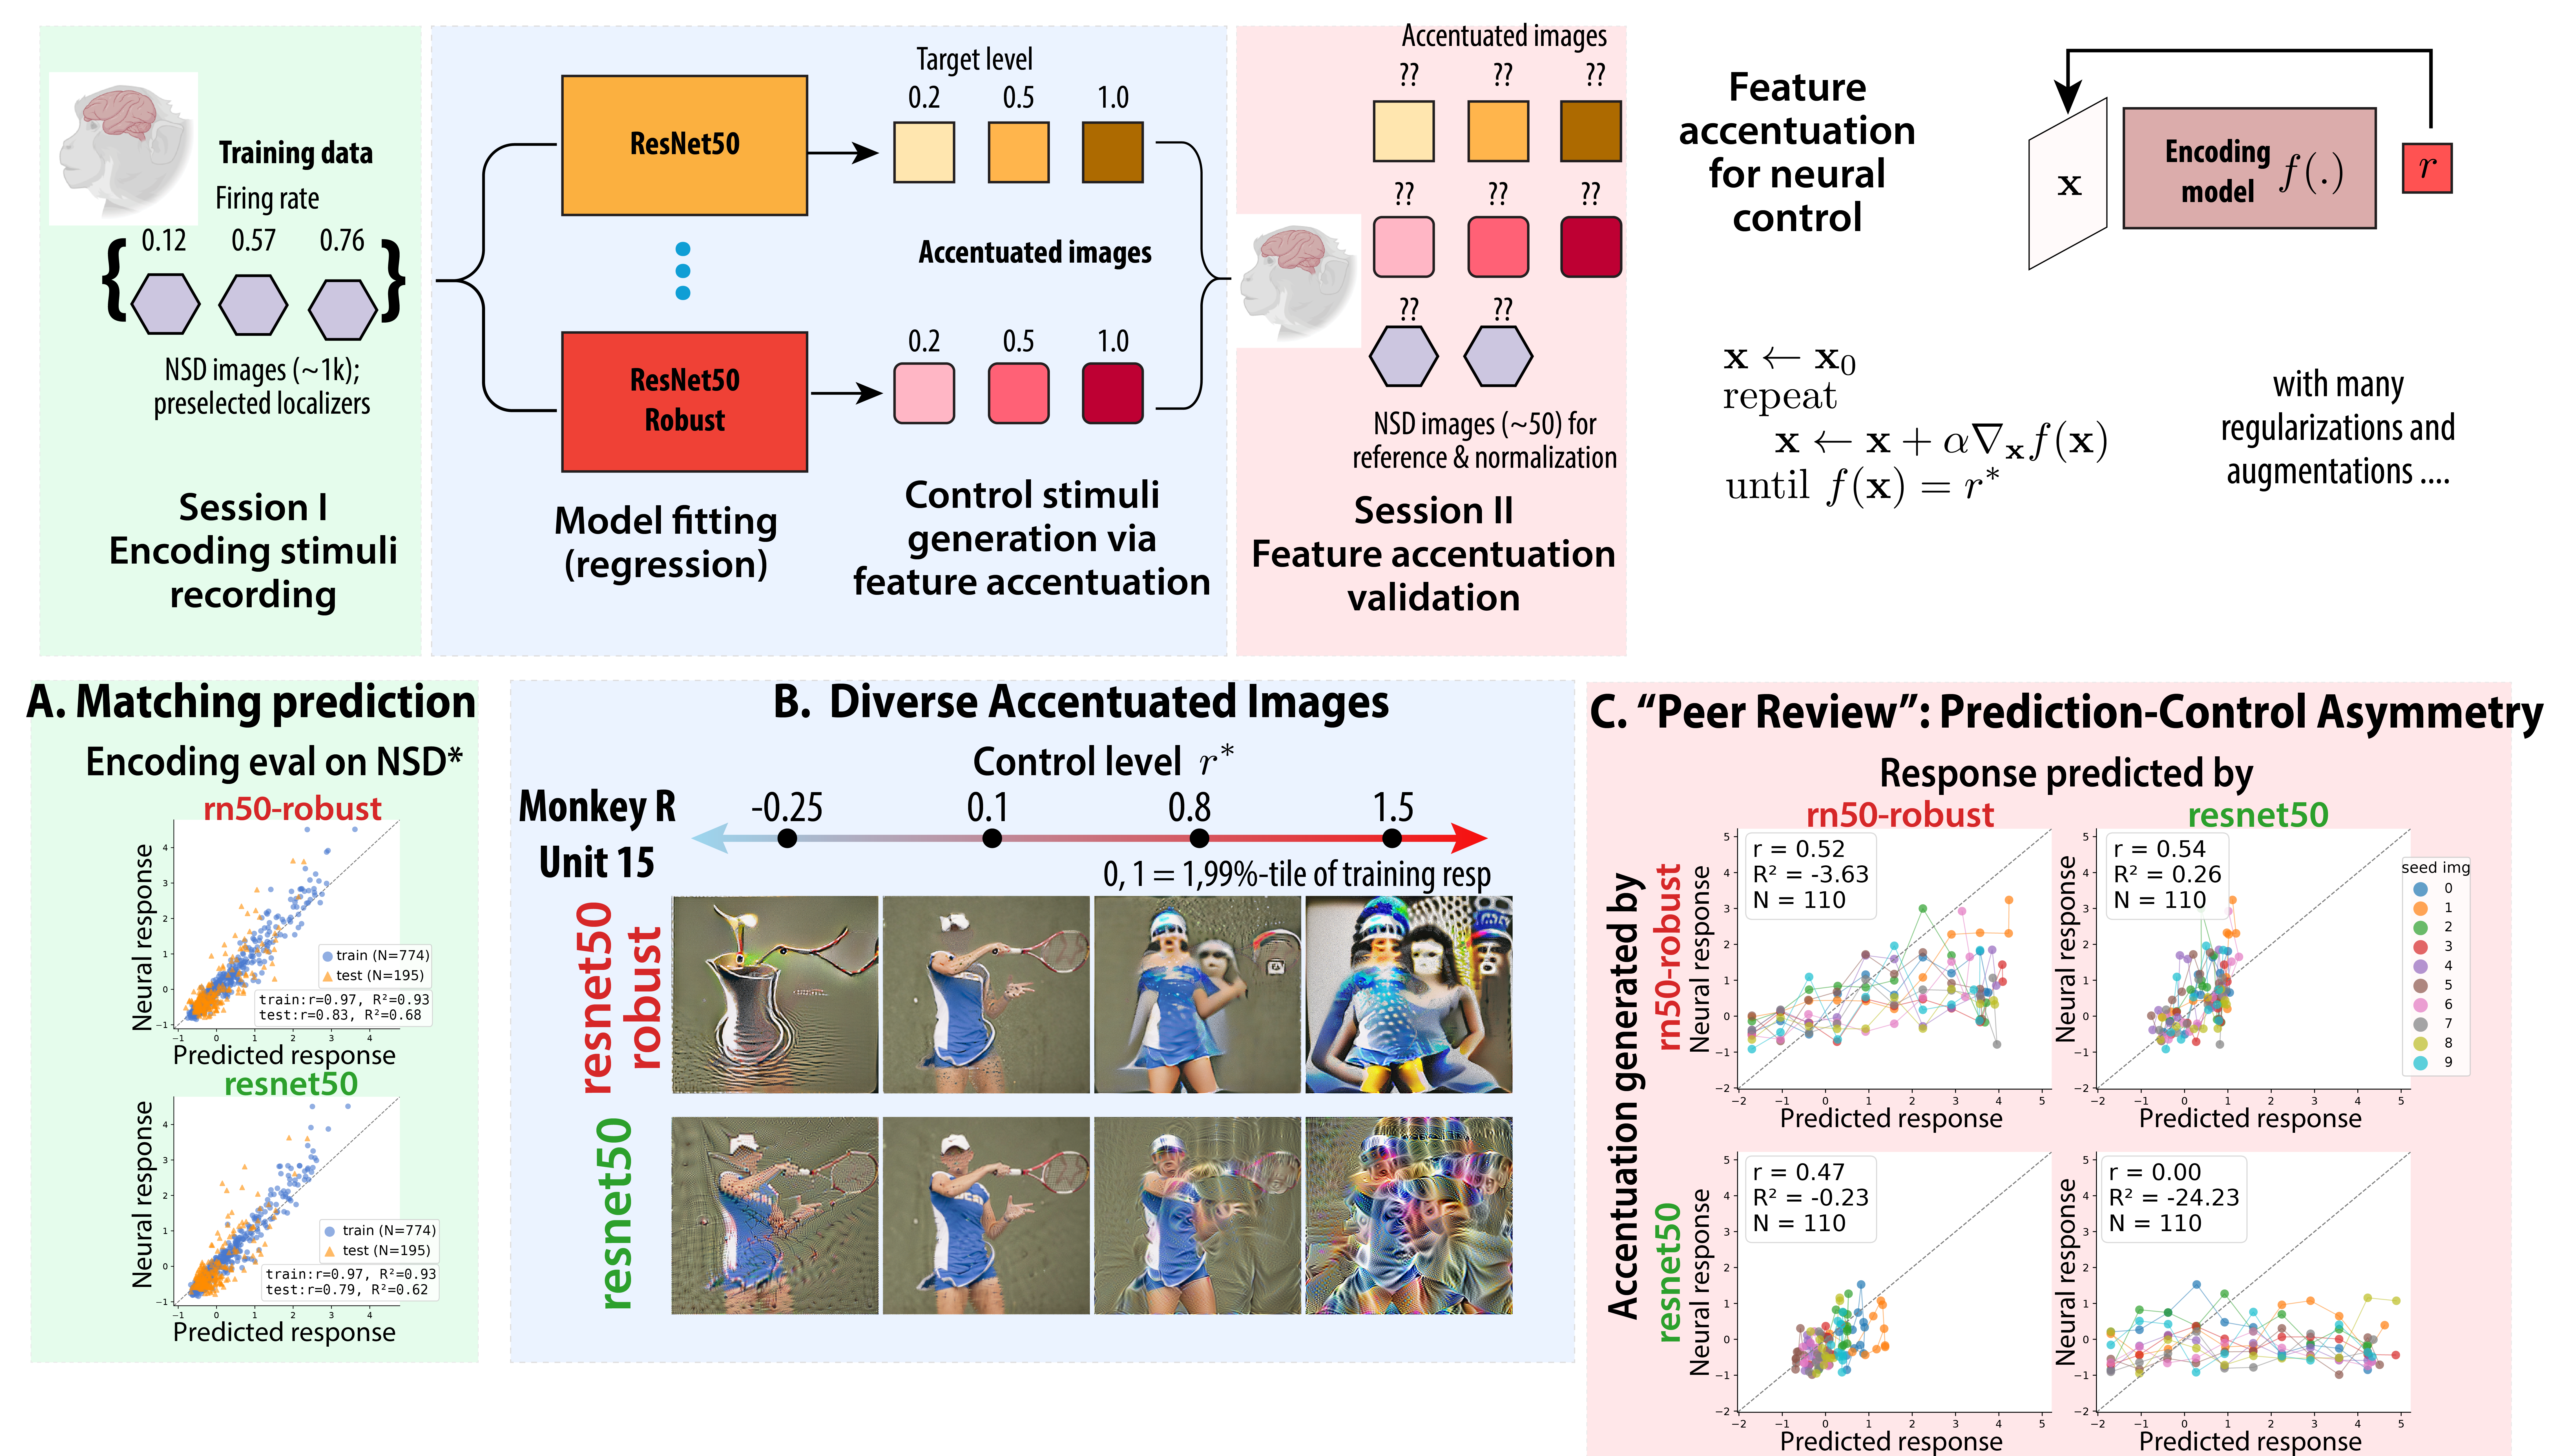
\includegraphics[width=\linewidth]{figures/Figure_NeuroCtrl_results.png}\\[2pt]
    % \vspace{-5pt}
    % 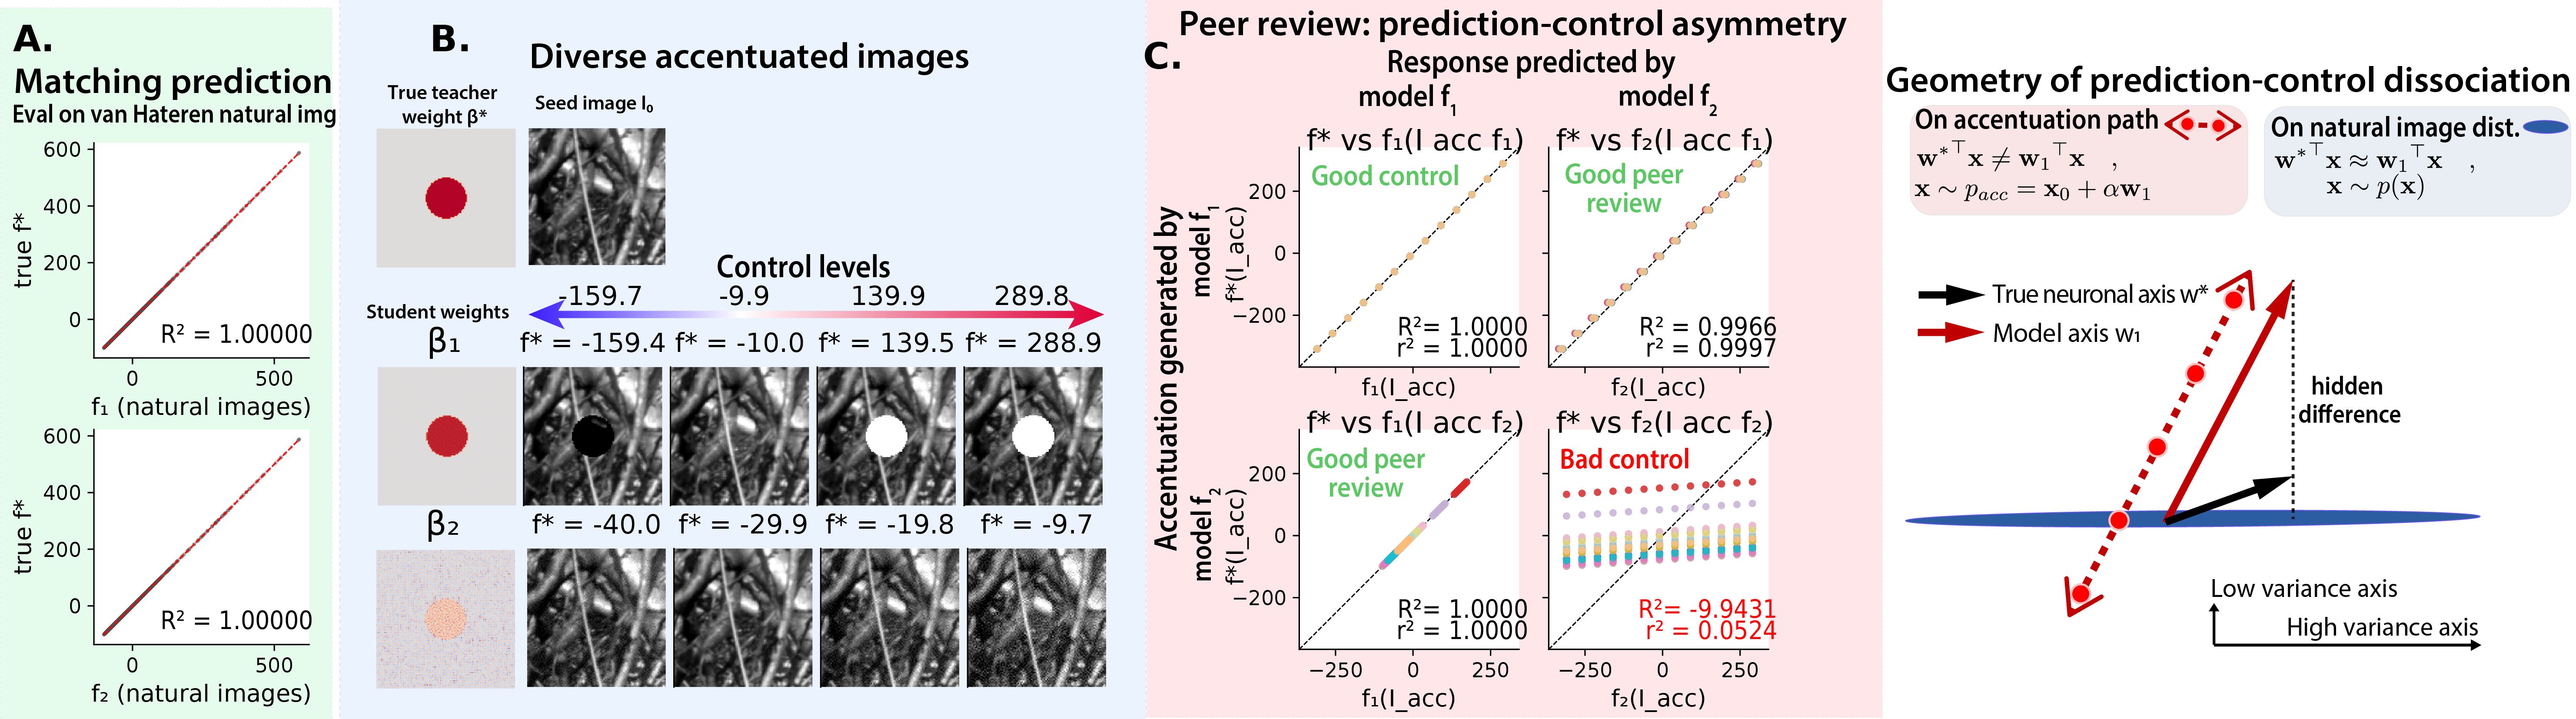
\includegraphics[width=\linewidth]{figures/Figure_LinearToyModel-04.png}
    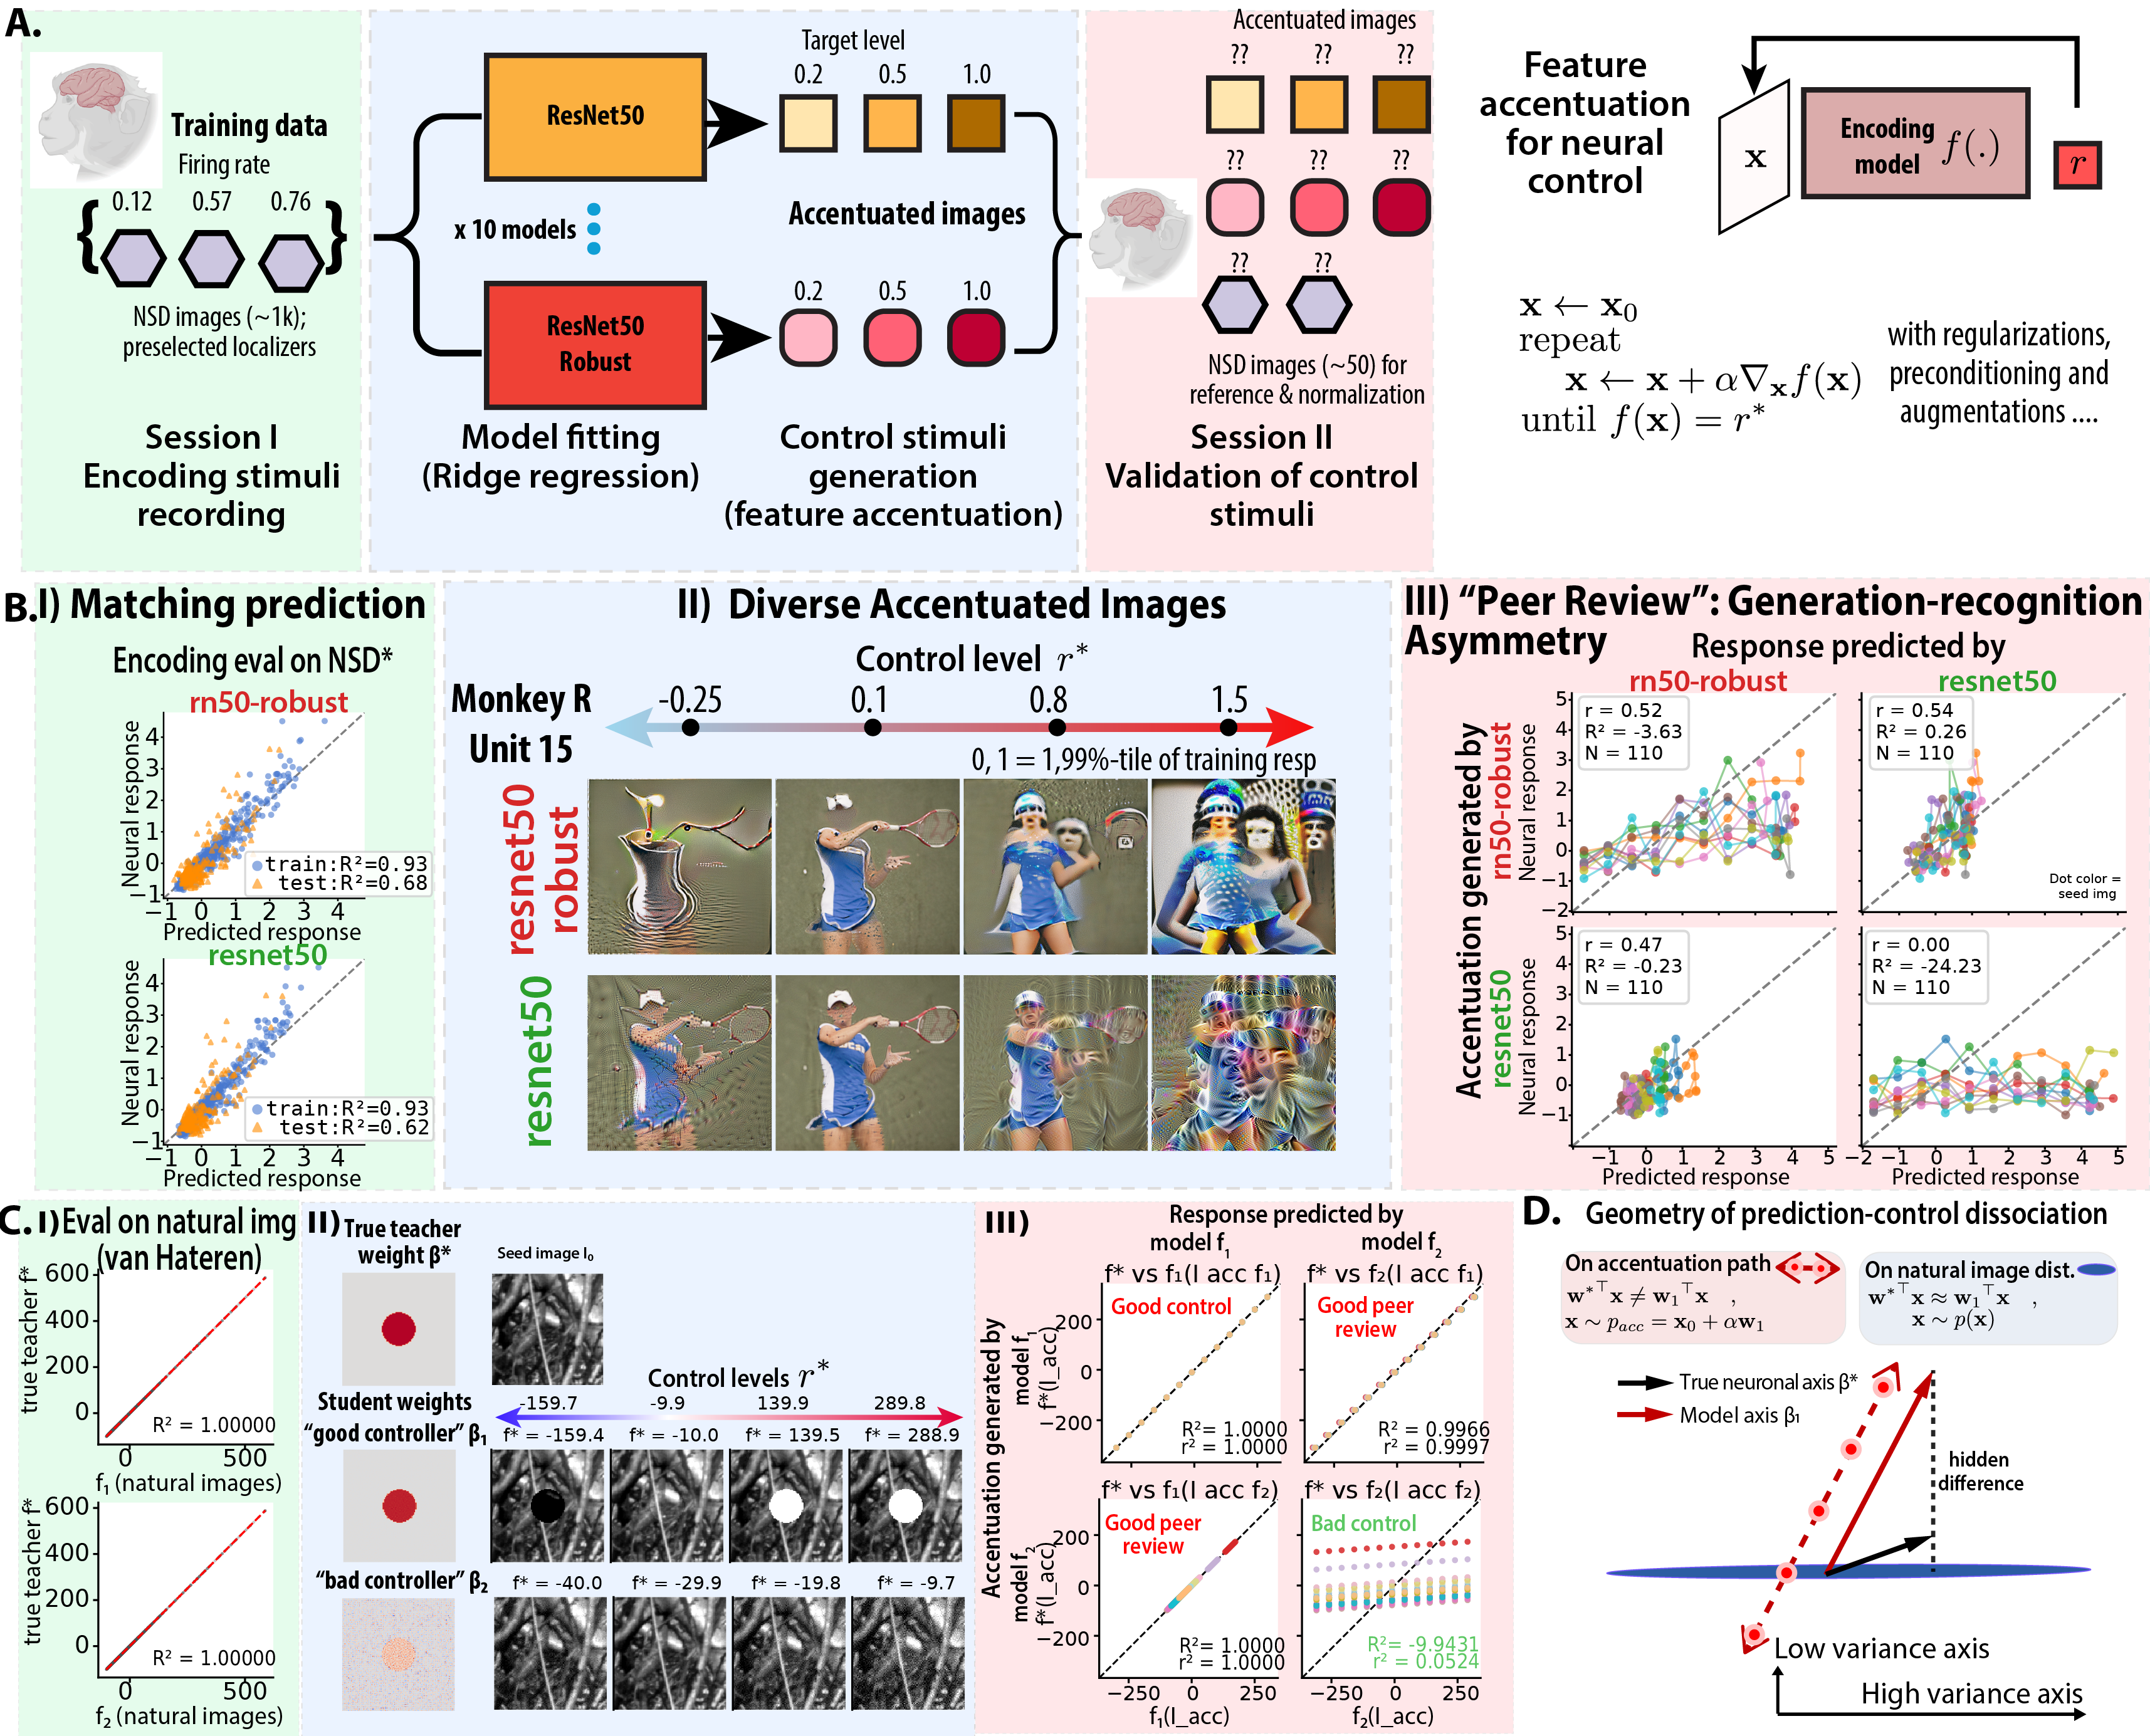
\includegraphics[width=\linewidth]{figures/Figure_NeuroCtrl_results_Neuro-linear-compose.png}
    \vspace{-10pt}
    \caption{\textbf{The dissociation of prediction and control in neurons and in a linear teacher--student model.}
    \textbf{A.} Closed-loop experiment of \citetPW. Encoding models are fit to responses to natural images, generate accentuated images for graded target responses, and are tested in a second session.
    \textbf{B.}
    \textbf{I}~Two models predict held-out natural-image responses equally well.
    \textbf{II}~Their accentuations from the same seed differ visibly.
    \textbf{III}~When each model evaluated on the other's images (\textit{peer review}), the weak controller (RN50) tracks neuronal responses on the strong controller's (RN50-robust) images but its own images barely modulate the neuron. % Only RN50-robust modulates the neuron.
    \textbf{C.}: two linear students of a linear teacher (a disk-shaped weight on van~Hateren images), weight differing along low-variance image directions, reproduce I-III qualitatively.
    \textbf{D.}: prediction on natural data hides weight error in small variance dim; the accentuation path exposes the hidden Euclidean difference.
    Methods see App.~\ref{sec:app-methods-neural-data}, ~\ref{sec:app-methods-toy} }
    %Details: App.~\ref{sec:app-methods-neural-data} (neurons), App.~\ref{sec:app-methods-toy} (linear model).}
    \label{fig:phenomena}
\end{figure}


\citetPW   used the following closed-loop paradigm (Fig.~\ref{fig:phenomena}, top): responses of visual cortical sites (V3/V4--IT, 25 sites in 5 macaques) to $\sim$1000 naturalistic images were recorded; for each site, ten encoding models were fit by ridge regression on the top 750 PCs of features from ten deep network backbones, with penalty and per-site layer chosen by cross-validation; using \emph{feature accentuation} \citep{hamblin2024feature}, each model optimized an image using a variant of gradient ascent, and then synthesized images that drive its own prediction to eleven target levels from ten seed images (Fig.~\ref{fig:phenomena}\textbf{A}); and the images were presented to the same sites in the \textit{control session}. The control is successful if the proposed images evoked neural activations as predicted (data and models: Apps.~\ref{sec:app-methods-neural-data},~\ref{sec:app-methods-models}). Three observations motivate this paper.

\paragraph{Similar prediction, divergent control.}
The trained models were tightly matched on held-out natural images (Fig.~\ref{fig:phenomena}\textbf{B.I}), yet the slope and correlation between predicted and measured responses to their own accentuated images varied widely across models, with far larger spread than on natural images. Many models reached their target \emph{predicted} response by adding texture and high-spatial-frequency structure that left the neuron largely unmoved (Fig.~\ref{fig:phenomena}\textbf{B.II}).

\paragraph{Recognition without generation.}
Presenting model A's images to model B (``peer review'', Fig.~\ref{fig:phenomena}\textbf{B.III}) shows an asymmetry: a model whose own images fail to modulate the neuron still predicts the neuronal responses to a successful model's images with good correlation and better $R^2$ than the generator itself. Models can recognize good control stimuli that they cannot produce.

\paragraph{Control tracks input-gradient structure.}
Across the 250 site--model pairs, control success is predicted by the spectral profile of the model's input gradient $\nabla_\x f$: models whose gradients concentrate power at low spatial frequencies, like natural images, control better. The two adversarially trained models are the strongest controllers, but the association persists without them \citepPW.

These phenomena are puzzling at first glance, but linear models on natural images reproduce all three observations (Fig.~\ref{fig:phenomena}\textbf{C}). We construct the bad controller to deviate from the teacher along the lowest-variance, high-spatial-frequency directions of the image covariance, the good controller to deviate mildly along mid-band PCs; then matched prediction, diverse accentuations, unequal control and good peer review all follow. Dissecting this idealistic set up, the rest of the paper explains why \textit{finite-sample} regression on \textit{noisy responses} produces such errors, why \textit{cross-validation does not remove them}, and how \textit{feature maps} can amplify the dissociation.

% These phenomena are puzzling at first glance, though we show, linear models on natural images can reproduce all three observations (\red{
% bottom, Fig.~\ref{fig:phenomena}}).
% We constructed the bad controller to have weight error along low-variance directions of the image covariance (high spatial frequency), while the good controller has weight error more along the high eigenspace. Then matched prediction on natural data; diverse generated images; unequal control outcomes and relatively good peer reviews all emerge from it.
% This shows the same symptom can emerge without deep network, nonlinearity or neurons.
% Dissecting this idealistic set up, the remainder of the paper explains why \textit{finite-sample} regression on \textit{noisy responses} produces this failure, why \textit{cross-validation does not eliminate it}, and how \textit{feature maps} introduce additional degrees of freedom that can greatly amplify the prediction--control dissociation.


\vspace{-15pt}
\section{Three evaluations, three geometries of one predictor}
\label{sec:setup}

\paragraph{Teacher and student.}
We idealize a visual neuron as a noisy linear teacher, its encoding model as a linear student, and natural image inputs as $\x\in\R^d,\x\sim\mathcal N(0,\Sigma)$, a centered Gaussian distribution with structured covariance $\Sigma=\sum_ks_k\uvec_k\uvec_k^\top$.
A linear teacher with weight $\bstar=\sum_kb_k\uvec_k$ produces noisy responses $y=\x^\top\bstar+\sigma\epsilon$, $\epsilon\sim\mathcal{N}(0,1)$, and $S:={\bstar}^\top\Sigma\bstar$ is the noiseless natural response variance.
The student is $f(\x)=\x^\top\bhat$, fitted from $n$ pairs $(X,\mathbf y)$; for linear feature-space students (Sec.~\ref{sec:feature}) $\bhat$ is the effective pixel weight $F^\top\hat w$, which is also the gradient $\nabla_\x f$.

\paragraph{Three distributions.}
Generalization evaluates $f$ on fresh natural inputs, $\x\sim\mathcal N(0,\Sigma)$. Accentuation evaluates $f$ on inputs it generates itself: gradient ascent from a seed $\x_0$ moves along $\nabla_\x f=\bhat$, so the idealized path is $\x=\x_0+\alpha\bhat$ with $\alpha$ set by the target level\footnotemark. %In the main text,
We study $\x_0=0$ and the target range is variance-matched, $\Var[\alpha]({\bhat}^\top\bhat)^2=S$, so the student's \emph{prediction} has natural dynamic range along its path. Peer review evaluates $f$ on the path $\x_0+\alpha\bprime$ generated by another student $\bprime$. Writing $\Delta=\bhat-\bstar$ and applying the standard formulas for MSE, $R^2$ and the slope of true-on-predicted response to each distribution (Lem.~\ref{lem:mr-metrics}) gives Table~\ref{tab:evaluation-metrics}.
\footnotetext{In practice, accentuation for DNN adds gradient preconditioning and augmentation \citep{hamblin2024feature,fel2023magnitudeConstrainedOptimization}, and some add image priors \citep{bashivan2019neuralPopulationControl}.} %App.~\ref{sec:app-evaluation-distributions} treats nonzero and multiple seeds.}

\begin{table}[t]
\vspace{-10pt}
\centering\footnotesize\setlength{\tabcolsep}{3.5pt}
\resizebox{\ifdim\width>\linewidth\linewidth\else\width\fi}{!}{%
\begin{tabular}{@{}llcccl@{}}
\toprule
Evaluation & Covariance & MSE $E$ & $R^2$ & Slope & Equal-error set \\
\midrule
Generalization & $\Sigma$ & $\Delta^\top\Sigma\Delta$ & $1-\Delta^\top\Sigma\Delta/S$ & ${\bhat}^\top\Sigma\bstar/{\bhat}^\top\Sigma\bhat$ & ellipsoid \\
Accentuation & $\Var[\alpha]\,\bhat{\bhat}^\top$ & $S\,(1-N/D)^2$ & $1-(D/N-1)^2$ & $N/D$ & sphere \\
Peer review & $\Var[\alpha']\,\bprime{\bprime}^\top$ & $S\,(D_{peer}-N_{peer})^2/\|\bprime\|^4$ & $1-(D_{peer}/N_{peer}-1)^2$ & $N_{peer}/D_{peer}$ & hyperplane \\
\bottomrule
\end{tabular}}
\caption{Evaluation metrics on three distributions, and their geometries. $\Delta:=\bhat-\bstar$; on the student's own path the true and predicted gains are $N:={\bhat}^\top\bstar$, $D:={\bhat}^\top\bhat$, and on a peer's path $N_{peer}:={\bstar}^\top\bprime$, $D_{peer}:={\bhat}^\top\bprime$; $z:=D/N-1$ in each row. Last column: level sets of each row's metrics in the space of student weights $\bhat$ (Prop.~\ref{prop:mr-iso-geometry}).}
% \caption{One fitted weight, three evaluation distributions, three geometries. $\Delta:=\bhat-\bstar$; on the student's own path the true and predicted gains are $N:={\bhat}^\top\bstar$, $D:={\bhat}^\top\bhat$, and on a peer's path $N_{peer}:={\bstar}^\top\bprime$, $D_{peer}:={\bhat}^\top\bprime$; $z:=D/N-1$ in each row. The last column is the level set of each row's metrics in the space of student weights $\bhat$: an ellipsoid about $\bstar$, a sphere on the diameter $[0,(1+z)\bstar]$, a hyperplane normal to $\bprime$ (Prop.~\ref{prop:mr-iso-geometry}). Pearson correlation is degenerate on a noiseless rank-one path and is omitted.}
\label{tab:evaluation-metrics}
\vspace{-17pt}
\end{table}

\paragraph{Prediction is covariance-weighted, control is Euclidean.}
Generalization error is $E_{gen}=\Delta^\top\Sigma\Delta$: a weight error $\Delta$ along $\uvec_k$ costs $s_k$ times its squared length, so errors in low-variance directions can be nearly invisible. For accentuation, weight error is evaluated on a single path $\bhat$, and every metric is a function of the scalar $z$, or equivalently the ratio between quadratic forms $D/N$,
\begin{equation}\small
z_{acc}:=\frac DN-1=\frac{{\bhat}^\top(\bhat-\bstar)}{{\bhat}^\top\bstar},
\qquad
\frac{E_{acc}}{S}=\Big(\frac{z}{1+z}\Big)^2,\quad R^2_{acc}=1-z^2,\quad \mathrm{slope}_{acc}=\frac{1}{1+z},
\label{eq:acc_metric_ND_depen}
\end{equation}
\begin{wrapfigure}[26]{r}{0.45\linewidth}
    \vspace{-8pt}
    \centering
    \vspace{-5pt}
    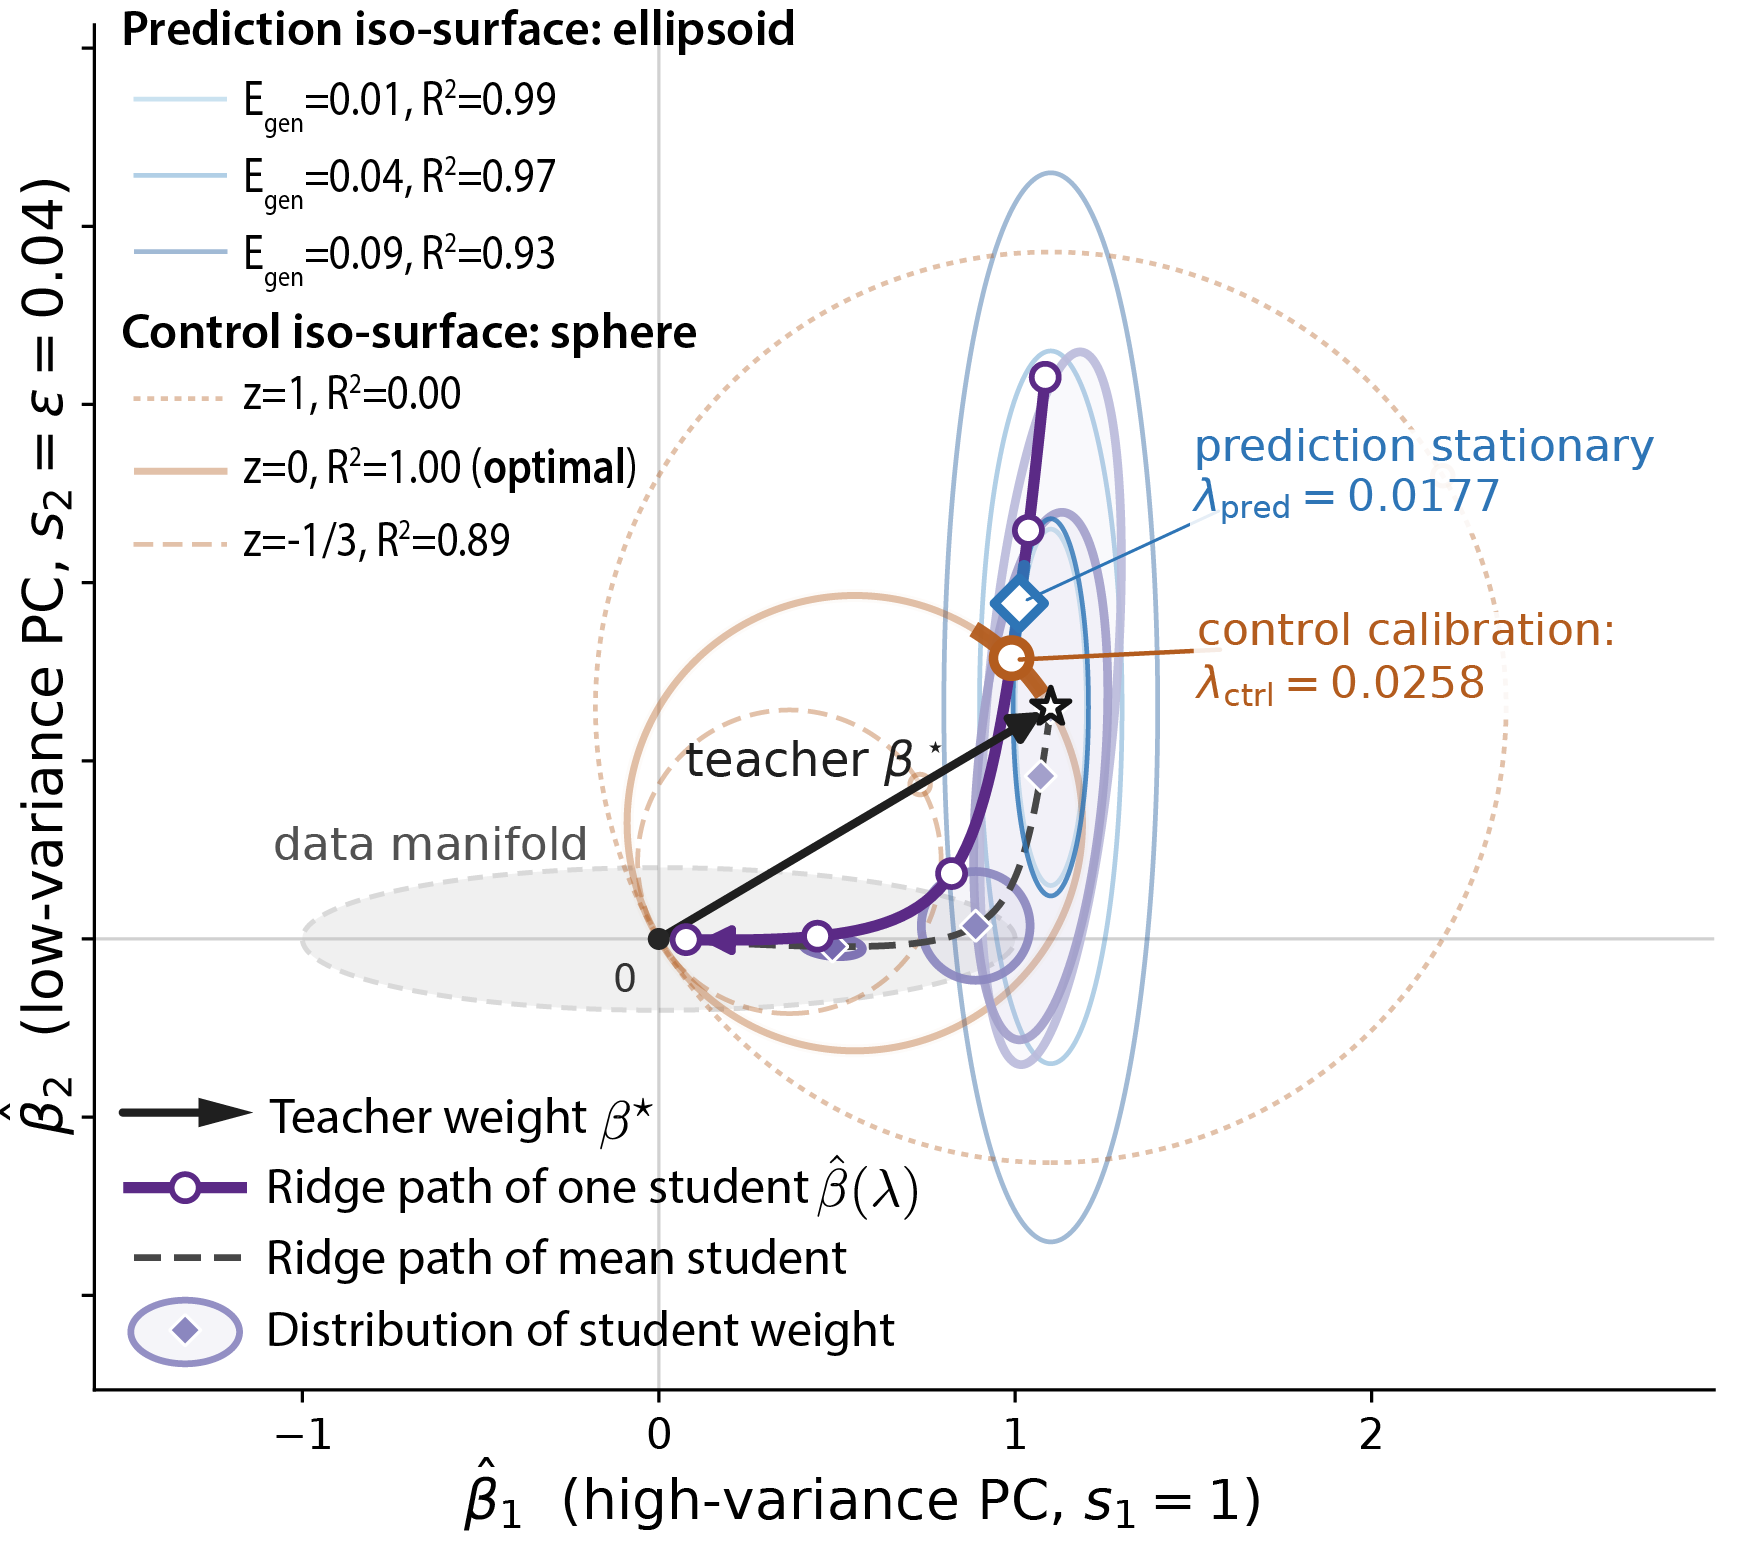
\includegraphics[width=\linewidth]{figures/Figure_iso_err_surf_dissociation-01.png}
    \vspace{-20pt}
    \caption{\textbf{Equal-error sets and the ridge path} in the plane of a high- and a low-variance PC. Prediction levels are ellipsoids around $\bstar$ (blue), control levels are the spheres with diameter joining $0$ and $(1+z)\bstar$ (orange). The fitted weight traverses this plane as a function of $\lambda$ (purple), scattering around the conditional-mean path (dashed black). The prediction-optimal penalty is the tangency of the path with an ellipsoid; perfect control is its crossing with the $z=0$ sphere. Exact two-dimensional construction: App.~\ref{sec:app-ext-geometry}. }
    \label{fig:geometry}
\end{wrapfigure}
The three evaluations therefore have three geometries in the space of student weights (Table~\ref{tab:evaluation-metrics}; Prop.~\ref{prop:mr-iso-geometry}; Fig.~\ref{fig:geometry}).
\textbf{Prediction: ellipsoids.} The equal-$E_{gen}$ sets are ellipsoids centered on $\bstar$ with semi-axis $\sqrt{E_{gen}/s_k}$ along $\uvec_k$, hence elongated along low-variance axes, where large weight errors are cheap.
\textbf{Control: spheres.} The equal-$z_{acc}$ sets are Euclidean spheres whose diameter joins $0$ and $(1+z)\bstar$; the diameter encodes the error directly, and zero-error students live on the sphere through $\bstar$ at $z=0$, not only at $\bstar$ itself.
\textbf{Peer review: hyperplanes.} The equal-$z_{peer}$ sets are hyperplanes normal to the generator $\bprime$, so a peer reviewer is judged only on its component along the peer's path.
A student can sit deep inside a small prediction ellipsoid, lie on a huge control sphere, and still lie on the zero-error hyperplane of a good generator: this is exactly the configuration of Fig.~\ref{fig:phenomena}\textbf{C}, and it can be made arbitrarily extreme by adding weight along a direction with $s_k\to0$ (Exp .~\ref{ex:mr-dissociation}).


The remaining question is therefore not whether the dissociation is possible but when \emph{learning} produces it. We study three ingredients: finite-sample regression on noisy responses, the choice of regularization, and the feature map through which the gradient reaches the pixels. % We take them in turn.

\vspace{-10pt}
\section{Pixel-space ridge: noise, spectrum and regularization}
\label{sec:pixel}

Ridge regression in pixel space, $\bhat=\arg\min_\beta\frac1n\|X\beta-\mathbf y\|^2+\lambda\|\beta\|^2$, yields
\begin{equation}
\bhat=\underbrace{(\hat\Sigma+\lambda I)^{-1}\hat\Sigma\bstar}_{\text{mean: signal shrinkage}}
+\underbrace{\sigma(\hat\Sigma+\lambda I)^{-1}\tfrac1nX^\top\eta}_{\text{noise}},
\qquad \hat\Sigma=X^\top X/n,
\quad
\mathbf y=X\bstar+\sigma \eta
\label{eq:ridge}
\end{equation}
% Since ridge penalizes weight in low-variance directions, one might expect it to remove these control-vulnerable weight components. We ask whether such risk survives the regularization, even with cross-validated penalty.
Since ridge penalizes weight in low-variance directions, one might expect it to remove these control-vulnerable components. We ask whether such control risk survive a cross-validated penalty.

\paragraph{The ridge path through the two landscapes.}
The question has a geometric reading (Fig.~\ref{fig:geometry}). For a given training set, Eq.~\ref{eq:ridge} traces a path $\bhat(\lambda)$ in weight space from the least-squares or minimum-norm solution at $\lambda\to0$ to the origin at $\lambda\to\infty$. Response noise and the random design scatter the fitted weight in a cloud around its mean. Ideally, cross-validation selects the point where the path is tangent to the smallest reachable prediction ellipsoid; whereas minimal control error asks where the path crosses the $z=0$ sphere $D=N$; in general these two points do not coincide. The analysis below makes this geometric picture quantitative.
%\red{the two coincide only if the noise cloud has not pushed the path off the sphere in the directions the ellipsoid does not see. The deterministic equivalents below compute where the center of this cloud sits, how much Euclidean spread it carries, and hence the distance between the two points.}, and the cloud is elongated along the low-variance directions of $\Sigma$, because those are the directions the data constrain least


\paragraph{Toolkit.}
We use deterministic equivalents (DEs) in the proportional limit $d/n\to\gamma$ \citep{dobriban2018high,hastie2022surprises}. They replace functions of the empirical covariance $\hat\Sigma$ by deterministic functions of the population covariance $\Sigma$, e.g. $\hat\Sigma(\hat\Sigma+\lambda I)^{-1}\asymp\Sigma(\Sigma+\kappa I)^{-1}$, where the finite-sample randomness is absorbed into an effective penalty $\kappa(\lambda)\ge\lambda$, the unique positive root of $\kappa-\lambda=\frac{\kappa}{n}\operatorname{Tr}[\Sigma(\Sigma+\kappa I)^{-1}]$, one-to-one in $\lambda$ (App.~\ref{sec:app-de-toolkit}).
Applied to Eq.~\ref{eq:ridge}, the DE says that the signal term concentrates around a \emph{mean fitted weight}, the teacher shrunk mode by mode,
\begin{equation}
\bar\beta_\kappa:=\Sigma(\Sigma+\kappa I)^{-1}\bstar=\sum_k\frac{s_k}{s_k+\kappa}\,b_k\uvec_k ,
\label{eq:pixel-mean-weight}
\end{equation}
% while the noise term has zero mean but carries Euclidean energy,
while the fluctuation around the mean causes the \emph{norm inflation} $V:=\E\|\bhat\|^2-\|\bar\beta\|^2\ge0$, which, as we will show, drives accentuation error. The mean weight $\bar\beta$ and inflation $V$ also organize the feature-space case and the nonlinear diagnostic (Secs.~\ref{sec:feature},~\ref{sec:nonlinear}). Results use the teacher-weighted and unweighted spectral sums
% We use deterministic equivalents (DEs) in the proportional limit $d/n\to\gamma$ \citep{dobriban2018high,hastie2022surprises}. They replace functions of the empirical covariance $\hat\Sigma$ by deterministic functions of the population covariance $\Sigma$, e.g. $\hat\Sigma(\hat\Sigma+\lambda I)^{-1}\asymp\Sigma(\Sigma+\kappa I)^{-1}$, where the finite-sample randomness is absorbed into an effective penalty $\kappa(\lambda)$. $\kappa$ can be found at the unique positive root of $\kappa-\lambda=\frac{\kappa}{n}\operatorname{Tr}[\Sigma(\Sigma+\kappa I)^{-1}]$, with $\kappa\ge\lambda$, and the mapping is one-to-one (App.~\ref{sec:app-de-toolkit}).
% DE allows us to study the average effect of a finite random design without requiring us to manipulate the realized matrix $X$ explicitly.
% Applied to Eq.~\ref{eq:ridge}, the DE says that the signal term concentrates around a \emph{mean fitted weight}, the teacher shrunk mode by mode,
% \begin{equation}
% \bar\beta_\kappa:=\Sigma(\Sigma+\kappa I)^{-1}\bstar=\sum_k\frac{s_k}{s_k+\kappa}\,b_k\uvec_k ,
% \label{eq:pixel-mean-weight}
% \end{equation}
% while the noise term has zero mean, but carries Euclidean energy. We call this energy the \emph{norm inflation}, $V:=\E\|\bhat\|^2-\|\bar\beta\|^2\ge0$. As we will see, it is the part of the fitted weight that can induce severe accentuation error. The same two objects, a mean weight $\bar\beta$ and an inflation $V$, will organize the feature-space case (Sec.~\ref{sec:feature}) and the nonlinear diagnostic (Sec.~\ref{sec:nonlinear}). Results are written with the teacher-weighted and unweighted spectral sums
\begin{equation}\small
B_{p,q}(\kappa)=\sum_k\frac{s_k^p}{(s_k+\kappa)^q}b_k^2,\qquad
\mathrm{df}_{p,q}(\kappa)=\sum_k\frac{s_k^p}{(s_k+\kappa)^q},\qquad \mathrm{df}_2:=\mathrm{df}_{2,2},
\end{equation}
so that, for instance, $\bstar^\top\bar\beta_\kappa=B_{1,1}$ and $\|\bar\beta_\kappa\|^2=B_{2,2}$.
For the ratio $N/D$ we use the leading approximation $\mu_N/\mu_D$ from the DEs of $N$ and $D$; second-order and distributional refinements matter only where the leading calibration error is already small (App.~\ref{sec:app-ratio-corrections}).

\begin{figure}[t]
    \centering
    \vspace{-19pt}
    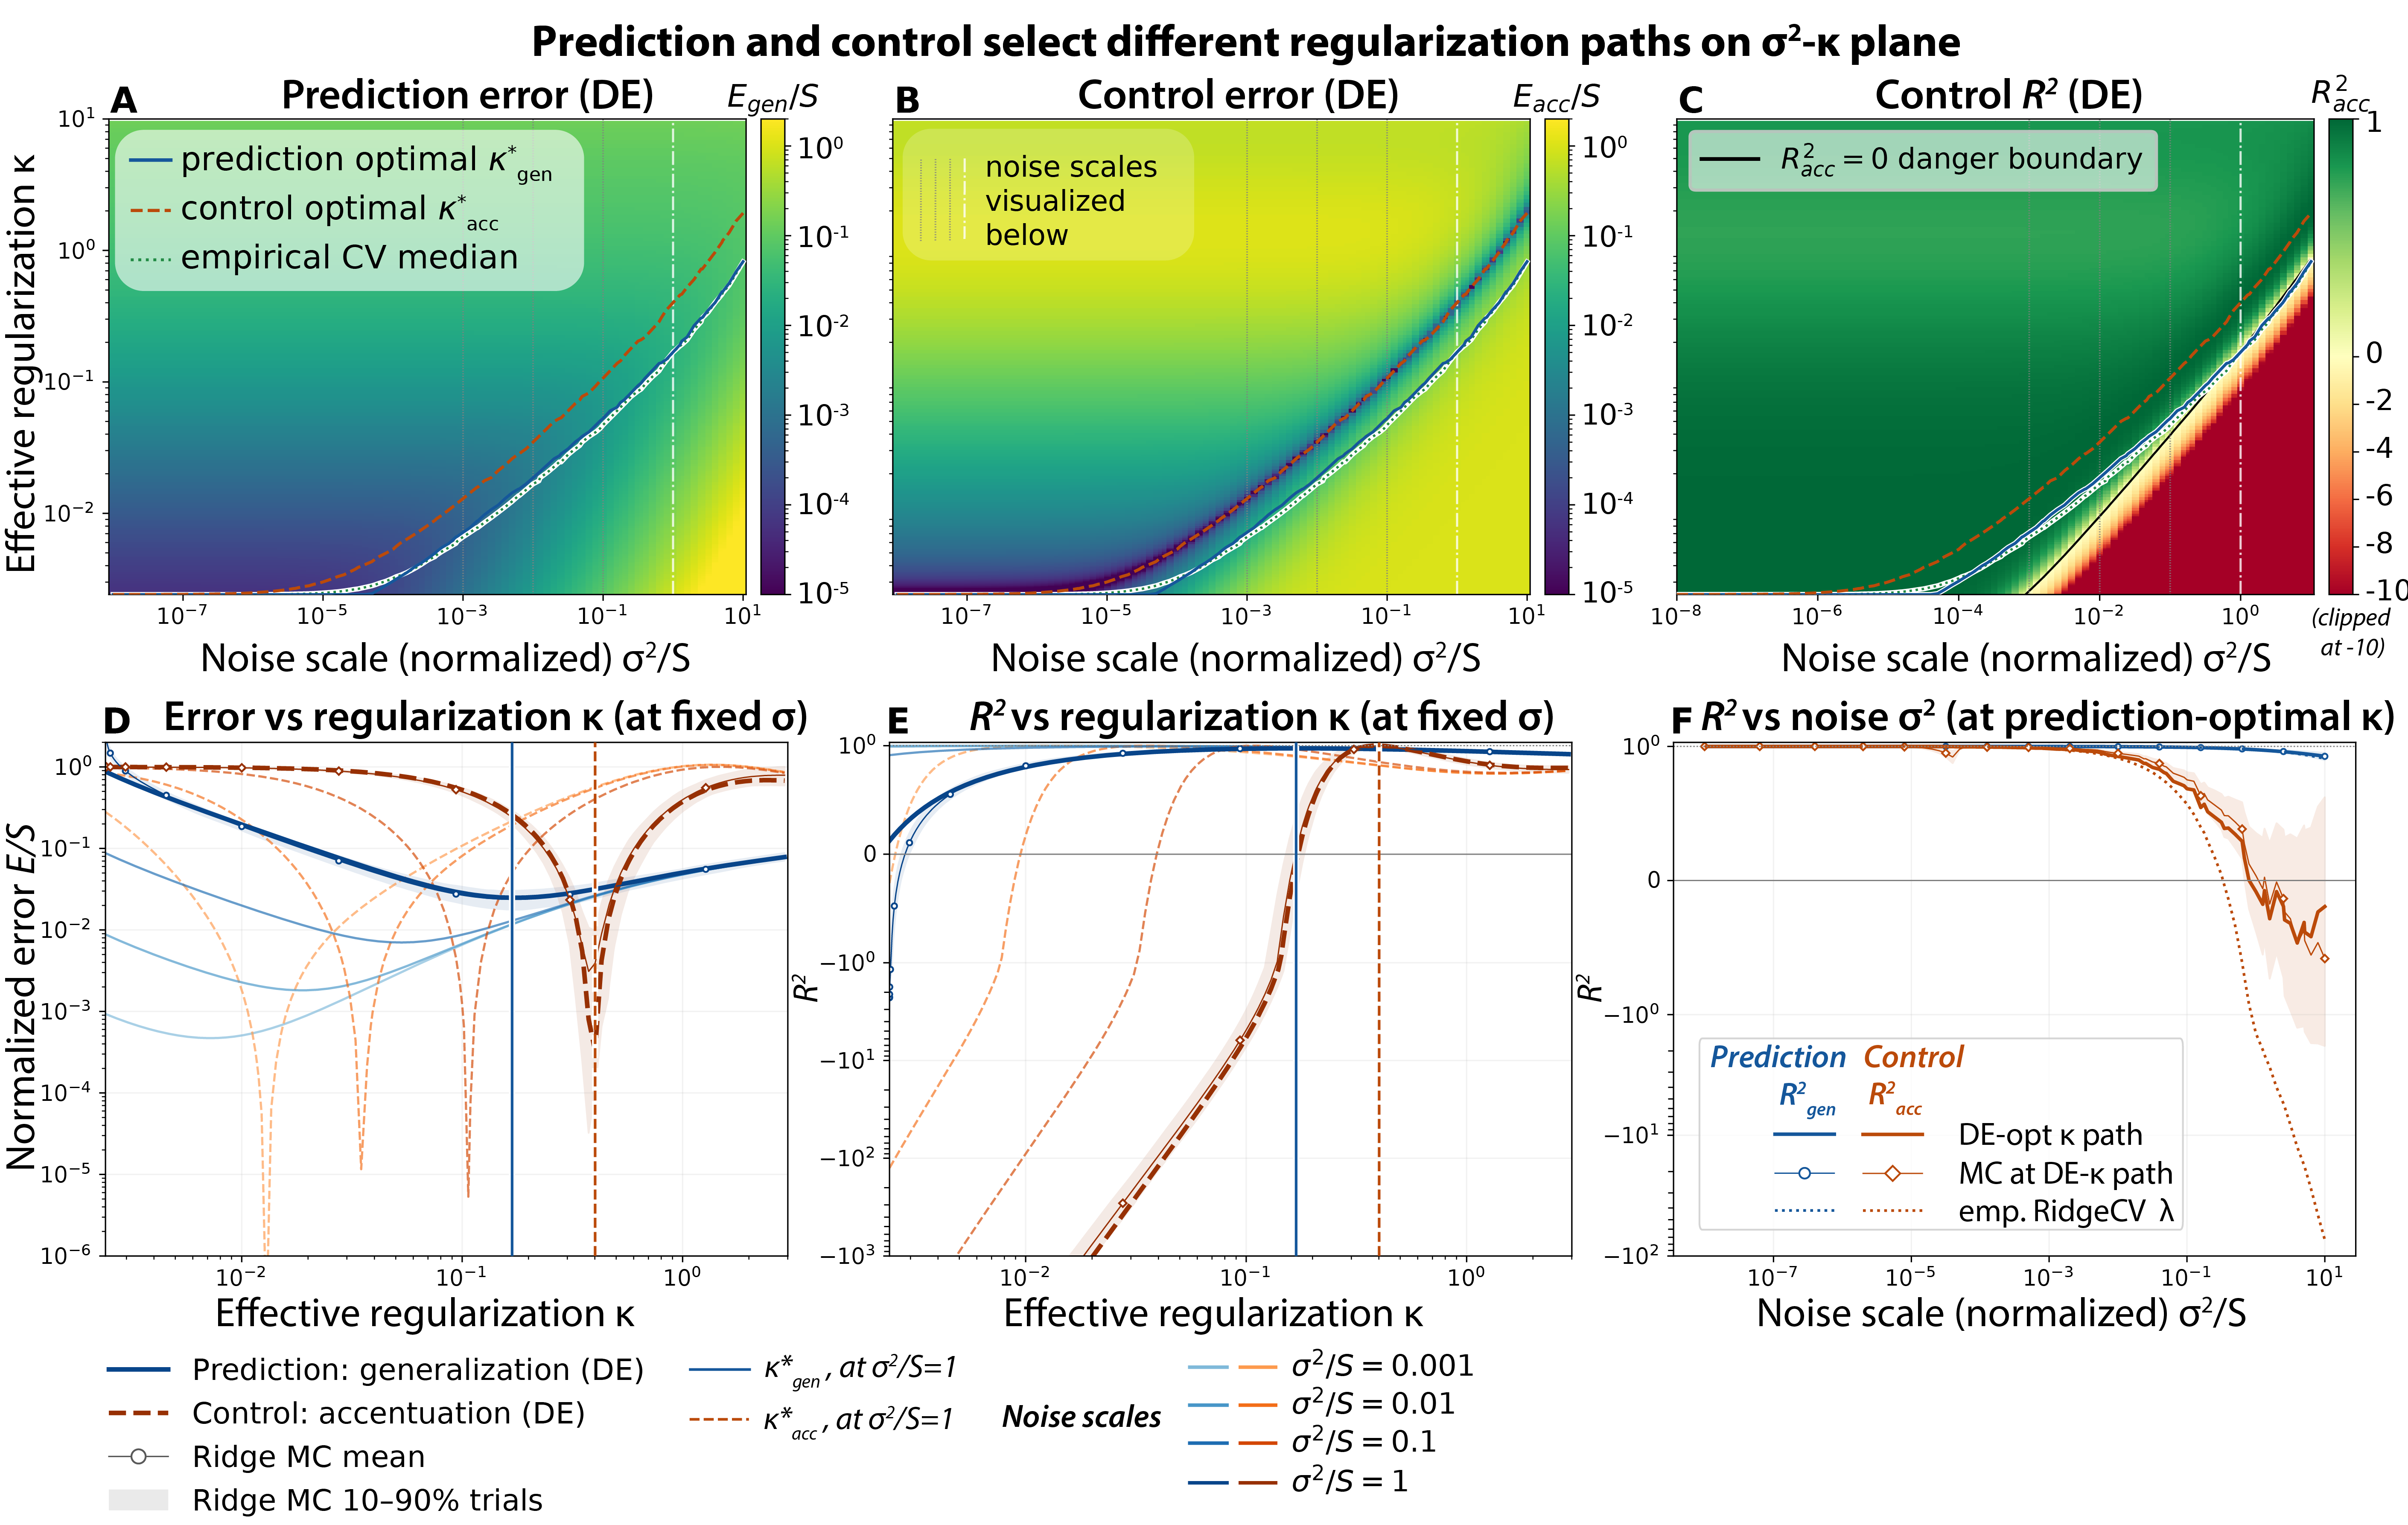
\includegraphics[width=\linewidth]{figures/Figure_PixRidgeGeometry.png}
    \vspace{-15pt}
    \caption{\textbf{Pixel-space ridge separates prediction- and control-optimal regularization on natural images.}
    Disk teacher on van~Hateren images ($d=10^4$, $n=10^3$).
    % \textbf{A--C}~The landscapes of prediction error $E_{gen}$, accentuation error $E_{acc}$, and accentuation $R^2$ over normalized noise scale $\sigma^2/S$ and effective regularization $\kappa$, calculated by DE (Eq.\ref{eq:pixel-de}). The prediction-optimal and median empirical RidgeCV paths track each other but differ from the control-optimal path; the black contour marks $R^2_{acc}=0$.
    % This picture is validated by the numerical MC estimated landscapes in \red{Fig.~\ref{fig:supp-pixel-de-mc}}.
    \textbf{A--C}~DE landscapes (Eq.~\ref{eq:pixel-de}) of $E_{gen}$, $E_{acc}$ and $R^2_{acc}$ over noise $\sigma^2/S$ and effective penalty $\kappa$ (Monte Carlo: Fig.~\ref{fig:supp-pixel-de-mc}). The prediction-optimal and median empirical RidgeCV paths track each other but not the control-optimal path; black contour: $R^2_{acc}=0$.
    \textbf{D,E}~Slices at four noise levels expose displaced prediction and control valleys (or peaks for $R^2$); markers and bands show the mean and 10--90\% range over 100 natural-image trials at the highlighted noise $\sigma^2/S=1$.
    \textbf{F}~Along the prediction-optimal path, $R^2_{gen}$ remains high while $R^2_{acc}$ becomes strongly negative; empirical RidgeCV exhibits the same dissociation. Methods see App.~\ref{sec:app-vanhateren-landscape-methods},~\ref{sec:app-ext-pixel}.}
    \vspace{-15pt}
    \label{fig:pixel}
\end{figure}

\begin{prop}[Pixel ridge: prediction and control]\label{prop:pixel-de}
With $\kappa$, $B$ and $\mathrm{df}$ built from $\Sigma$,
\begin{equation}
\begin{aligned}
E_{gen}&\asymp E_{gen,DE}=\frac{n(\kappa^2B_{1,2}+\sigma^2)}{n-\mathrm{df}_2}-\sigma^2,\qquad
N\asymp \mu_N=\bstar^\top\bar\beta_\kappa=B_{1,1},\\
D&\asymp \mu_D=\|\bar\beta_\kappa\|^2+V_{\rm pix}(\kappa),
\qquad
V_{\rm pix}(\kappa)=\frac{\mathrm{df}_{1,2}(\kappa)}{n}\big(E_{gen,DE}+\sigma^2\big).
\end{aligned}
\label{eq:pixel-de}
\end{equation}
(Proofs and the per-mode decomposition behind these sums: App.~\ref{sec:app-pixel-ridge}.)
\end{prop}
$E_{gen}$ recovers the classical in-distribution generalization error \citep{dobriban2018high,hastie2022surprises}. The two control moments have a plain reading. $N$ is the alignment of the teacher with the mean fitted weight, and the first term of $D$ is that weight's squared norm; both are set by the teacher and the shrinkage alone, and since each factor $s_k/(s_k+\kappa)$ lies in $[0,1]$ they are ordered $\|\bstar\|^2\ge B_{1,1}\ge B_{2,2}$ (Eq.~\ref{eq:app-spectral-inequalities}), so the mean weight by itself \emph{under}-shoots its own path ($D<N$, slope above one). The second term of $D$ is the key issue. $V_{\rm pix}$ summarizes how limited data $n$, response noise $\sigma^2$ and prediction error $E_{gen}$ jointly inflate the student norm, amplified by the spectral susceptibility $\mathrm{df}_{1,2}=\sum_ks_k/(s_k+\kappa)^2$, which counts the number of modes near the regularization threshold $\kappa$.
Inflation enlarges $D$ without changing $N$, so the student can easily \emph{over}-predict: $\mathrm{slope}_{acc}=N/D$ drops below one, and $z=D/N-1$ can grow until $R^2_{acc}=1-z^2$ turns negative.
Note that $V$ is not necessarily bad for control: at the special point $B_{1,1}=B_{2,2}+V_{\rm pix}$ the inflation exactly replenishes the norm lost to shrinkage, so $N=D$ and control is perfect at leading order (the valley in Fig.~\ref{fig:pixel}\textbf{B}).
This is generally not where cross-validation lands, as the next proposition shows.
%that, for a natural-image spectrum, accumulates over thousands of weakly constrained high-frequency modes

\begin{prop}[Prediction-optimal and control-optimal penalties differ]\label{prop:pixel-tuning}
Among admissible values of $\kappa$, let $\kappa_{\rm gen}^{\star}$ be an
interior differentiable minimizer of $E_{\rm gen,DE}$, and let
$\kappa_{\rm acc}^{\star}$ denote a zero of the leading control error,
equivalently satisfying $\mu_D=\mu_N$. Their defining conditions are
\begin{align}\small
E_{\rm gen,DE}+\sigma^2
&=n\kappa\frac{B_{2,3}}{\mathrm{df}_{2,3}},
&&(\kappa=\kappa_{\rm gen}^{\star};\ \text{prediction stationarity}),
\label{eq:gen_optim_reg_cond}\\
E_{\rm gen,DE}+\sigma^2
&=n\kappa\frac{B_{1,2}}{\mathrm{df}_{1,2}},
&&(\kappa=\kappa_{\rm acc}^{\star};\ \text{zero leading control error}).
\label{eq:acc_optim_reg_cond1}
\end{align}
% An interior minimizer of $E_{gen,DE}$ and a zero of the leading control error satisfy, respectively,
% \begin{equation}
% E_{gen,DE}+\sigma^2=n\kappa\frac{B_{2,3}}{\mathrm{df}_{2,3}}
% \quad\text{(prediction)},\qquad
% E_{gen,DE}+\sigma^2=n\kappa\frac{B_{1,2}}{\mathrm{df}_{1,2}}
% \quad\text{(control)},
% \label{eq:acc_optim_reg_cond1}
% \end{equation}
Further, at the prediction optimum $\kappa_{\rm gen}^{\star}$ the control error is
\begin{equation}\small
z^{(0)}_{acc,CV}=\frac{\kappa\,\mathrm{df}_{1,2}}{B_{1,1}}
\left(\frac{B_{2,3}}{\mathrm{df}_{2,3}}-\frac{B_{1,2}}{\mathrm{df}_{1,2}}\right)_{\kappa=\kappa^\star_{gen}} .
\label{eq:pixel-zacc-cv}
\end{equation}
(Proofs: App.~\ref{sec:app-optimal-regularization}.)
\end{prop}
Geometrically, along the ridge path (Fig.~\ref{fig:geometry}), $\kappa_{\rm gen}^{\star}$ lands at the tangency with the prediction ellipsoid and $\kappa_{\rm acc}^{\star}$ at its crossing of the control sphere.
Both conditions equate the noisy prediction risk to $n\kappa$ times a spectral-band average of the teacher's per-mode power $b_k^2$, but the two bands sit at different places (Fig.~\ref{fig:app-tuning-kernels}). The control kernel $s_k/(s_k+\kappa)^2$ is a bump centered at $s_k=\kappa$, symmetric on a log axis; the prediction kernel $s_k^2/(s_k+\kappa)^3$ is the same bump multiplied by the shrinkage factor $s_k/(s_k+\kappa)$, which shifts it up to $s_k\approx2\kappa$ and suppresses its low-variance side.
% \red{Each kernel is a $\kappa$-sensitivity: the control condition asks which modes' shrinkage $s_k/(s_k+\kappa)$ changes as $\kappa$ moves, since that sets the mean weight $\bar\beta_\kappa$ and $N$, whereas prediction stationarity asks which modes' \emph{squared} shrinkage changes, since that sets $E_{gen}$.}
Consequently $z^{(0)}_{acc,CV}$ compares the teacher power around $2\kappa$ with that around $\kappa$.
It vanishes for isotropic data, or for a teacher whose per-mode power $b_k^2$ is constant across modes. % (\todo{Rem.~\ref{rem:app-tuning-remarks}}).
For \textit{an anisotropic spectrum and a structured teacher} the averages differ, and their difference is the control error left at the cross-validated penalty. When $b_k^2$ decreases toward the low-variance tail, as for a teacher aligned with high-variance image modes, $z^{(0)}_{acc,CV}>0$ and the cross-validated student over-predicts ($\mathrm{slope}_{acc}<1$). %For \textit{an anisotropic spectrum and a structured teacher} the two averages differ generally, and their difference is the control error left at the cross-validated penalty. Notably, when $b_k^2$ decreases toward the low-variance tail, as for a teacher aligned with the high variance image modes, $z^{(0)}_{acc,CV}>0$ is positive, and the cross-validated student over-predicts ($\mathrm{slope}_{acc}=1/(1+z)<1$).

% ; and it is negative in the opposite case.
 %teacher-weighted spectral average $B_{,}$, but they average with different powers of $s_k/(s_k+\kappa)$.
% Eq.~\ref{eq:pixel-zacc-cv} is the distance along the path between its tangency with the prediction ellipsoid and its crossing of the control sphere.
%The gap is multiplied by $\kappa\,\mathrm{df}_{1,2}$, i.e. by the number of modes near the regularization edge.

Over the noise--regularization plane for natural images (Fig.~\ref{fig:pixel}\textbf{A--C}), the DE tracks Monte Carlo except at very low noise or regularization (Fig.~\ref{fig:supp-pixel-de-mc}). Prediction- and control-optimal penalties form two distinct valleys, the $E_{acc}$ valley a sharp cusp. At low noise, $\kappa^\star_{\rm gen}$ is also benign to control; as noise grows it approaches and crosses the $R^2_{acc}=0$ cliff, and control fails catastrophically. % tightened
% We visualize the landscape of prediction and control error over the noise-regularization plane ($\sigma^2,\kappa$), for regression on natural images (Fig.~\ref{fig:pixel}A-C).
% Our DE formula generally well tracks the Monte Carlo estimate of the error (Fig.~\ref{fig:supp-pixel-de-mc}), where deviation from leading DE occurs only at very low noise or low regularization cases.
% The prediction-optimal and control-optimal penalties form two distinct valleys, where the $E_{acc}$ valley is a cusp and much sharper than $E_{gen}$.
% At lower noise, prediction-optimal $\kappa^\star_{\rm gen}$ is also benign to control; however, at higher noise, $\kappa^\star_{\rm gen}$ gradually approaches and crosses the cliff of $R^2_{acc}=0$ , and control error fails catastrophically.

% Figure~\ref{fig:pixel} confirms the picture on real natural-image regression. The DE surfaces track Monte Carlo over eight decades of noise; the prediction-optimal and control-calibrated penalties form two distinct ridges; and along the cross-validated path the student remains an excellent predictor while its accentuation $R^2$ becomes negative at moderate noise.

% \red{In Fig.~\ref{fig:geometry}, Eq.~\ref{eq:pixel-zacc-cv} is the distance along the path between its tangency with the prediction ellipsoid and its crossing of the control sphere.}
This answers the question in the title for pixel regression: \emph{control is bad, despite prediction-optimal regularization, when the response is noisy, the spectrum is anisotropic, and many modes sit near $\kappa$}, which is exactly the noisy neuron with natural-image regime.



\paragraph{Peer review: recognition without generation.}
Peer review evaluates $\bhat$ on the path of a peer $\bprime$, so the roles of $N$ and $D$ are played by the true and predicted gains along the peer's path, $N_{peer}={\bstar}^\top\bprime$ and $D_{peer}={\bhat}^\top\bprime$ of Table~\ref{tab:evaluation-metrics}. Take the peer to be a ridge fit at the same $\kappa$ on independent data. Both fits then concentrate around the same mean weight $\bar\beta_\kappa$ while their noise parts are uncorrelated, so the norm inflation drops out of the cross product: $D_{peer}\asymp\|\bar\beta_\kappa\|^2=B_{2,2}$ and $N_{peer}\asymp\bstar^\top\bar\beta_\kappa=B_{1,1}$ (Prop.~\ref{prop:mr-peer}). The peer slope and score are therefore
\begin{equation}
\mathrm{slope}_{peer}=\frac{N_{peer}}{D_{peer}}\asymp\frac{B_{1,1}}{B_{2,2}}\in[1,\infty),
\qquad
R^{2,(0)}_{peer}=1-\Big(1-\frac{B_{2,2}}{B_{1,1}}\Big)^2\in(0,1],
\label{eq:peer-de}
\end{equation}
using $B_{1,1}\ge B_{2,2}$ (Eq.~\ref{eq:app-spectral-inequalities}). Note, on the leading order, the peer slope is never below one, i.e. the \textit{student under-predicts the teacher on its peer's path}, and the peer $R^2$ is non-negative and degrades gracefully with noise through the selected $\kappa$. In contrast, on the self-generated path the norm inflation $V_{\rm pix}$ of Eq.~\ref{eq:pixel-de} adds to $D$ but not to $N$:
%in terms of $z=D/N-1$, $z_{acc}\asymp z_{peer}+V_{\rm pix}/B_{1,1}$ with $z_{peer}=B_{2,2}/B_{1,1}-1\le0$,
so the student over-predicts the teacher ($\mathrm{slope}_{acc}=N/D<1$), and $z_{acc}$ can grow without bound, driving $R^2_{acc}$ negative.
The sign differences in neural data confirm this leading order picture: in \citetPW, peer-review scores between pairs of models have $R^2=0.04,[-0.06,0.10]$, $\mathrm{slope}=1.35,[1.14,1.59]$ (median, [IQR], $n=90$), whereas self-evaluation scores have $R^2=-4.17,[-4.59,-3.51]$, $\mathrm{slope}=0.38,[0.33,0.42]$ ($n=10$; App.~\ref{sec:app-ext-peer}, analysis in App.~\ref{sec:app-methods-peer}). % stats test between the two \todo
Note, in simplistic pixel space peer review, the slope and $R^2$ are symmetric between models ($A\leftarrow B$ or $B\leftarrow A$). In practice the students are fitted to the same recordings through different feature maps; the review score then becomes asymmetric, and the evaluator can recognize its own noise in the generator's path only to the extent that the two maps route noise into the same pixel directions (Sec.~\ref{sec:feature}; App.~\ref{sec:app-peer-shared}).
% Peer review measures only the shared shrinkage bias: at leading order it is never negative, degrades gracefully with noise, and is symmetric between the two fits. Self-evaluation instead carries the estimator's own Euclidean noise energy through Eq.~\ref{eq:pixel-de}, so $z_{acc}$ grows without bound with $\sigma^2/n$ and $R^2_{acc}$ becomes arbitrarily negative. A student can therefore track a peer's path while failing on its own, which is the linear form of Fig.~\ref{fig:phenomena}C.
% The asymmetry between a strong and a weak generator in the data arises when the two differ in their feature maps (Sec.~\ref{sec:feature}); %and measured responses along a barely modulated path add trial noise that no evaluator can explain, which is why even the peer scores of a weak generator's images are poor.

\begin{figure}[tp]
    \centering
    \vspace{-15pt}
    % 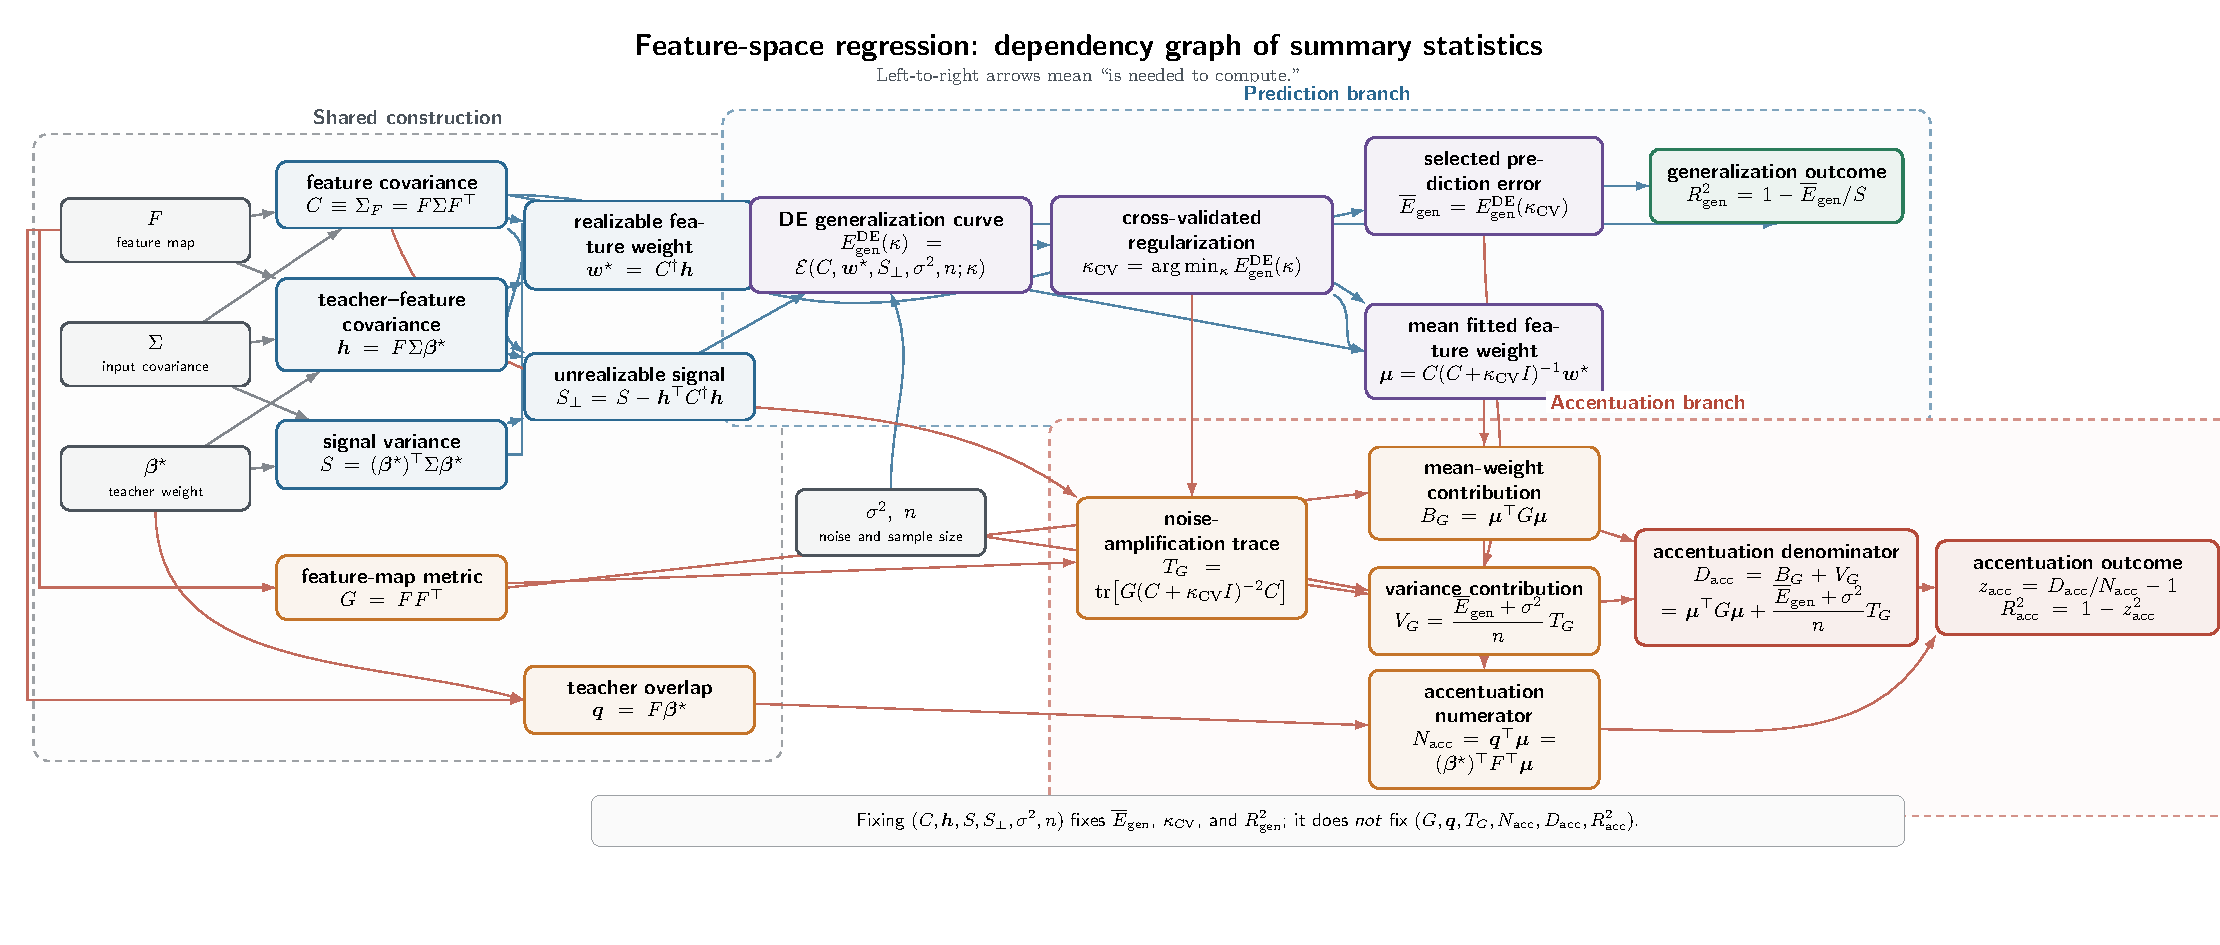
\includegraphics[width=0.55\linewidth,height=0.22\textheight,keepaspectratio]{figures/feature_summary_statistics_flow.pdf}%\hfill
    % 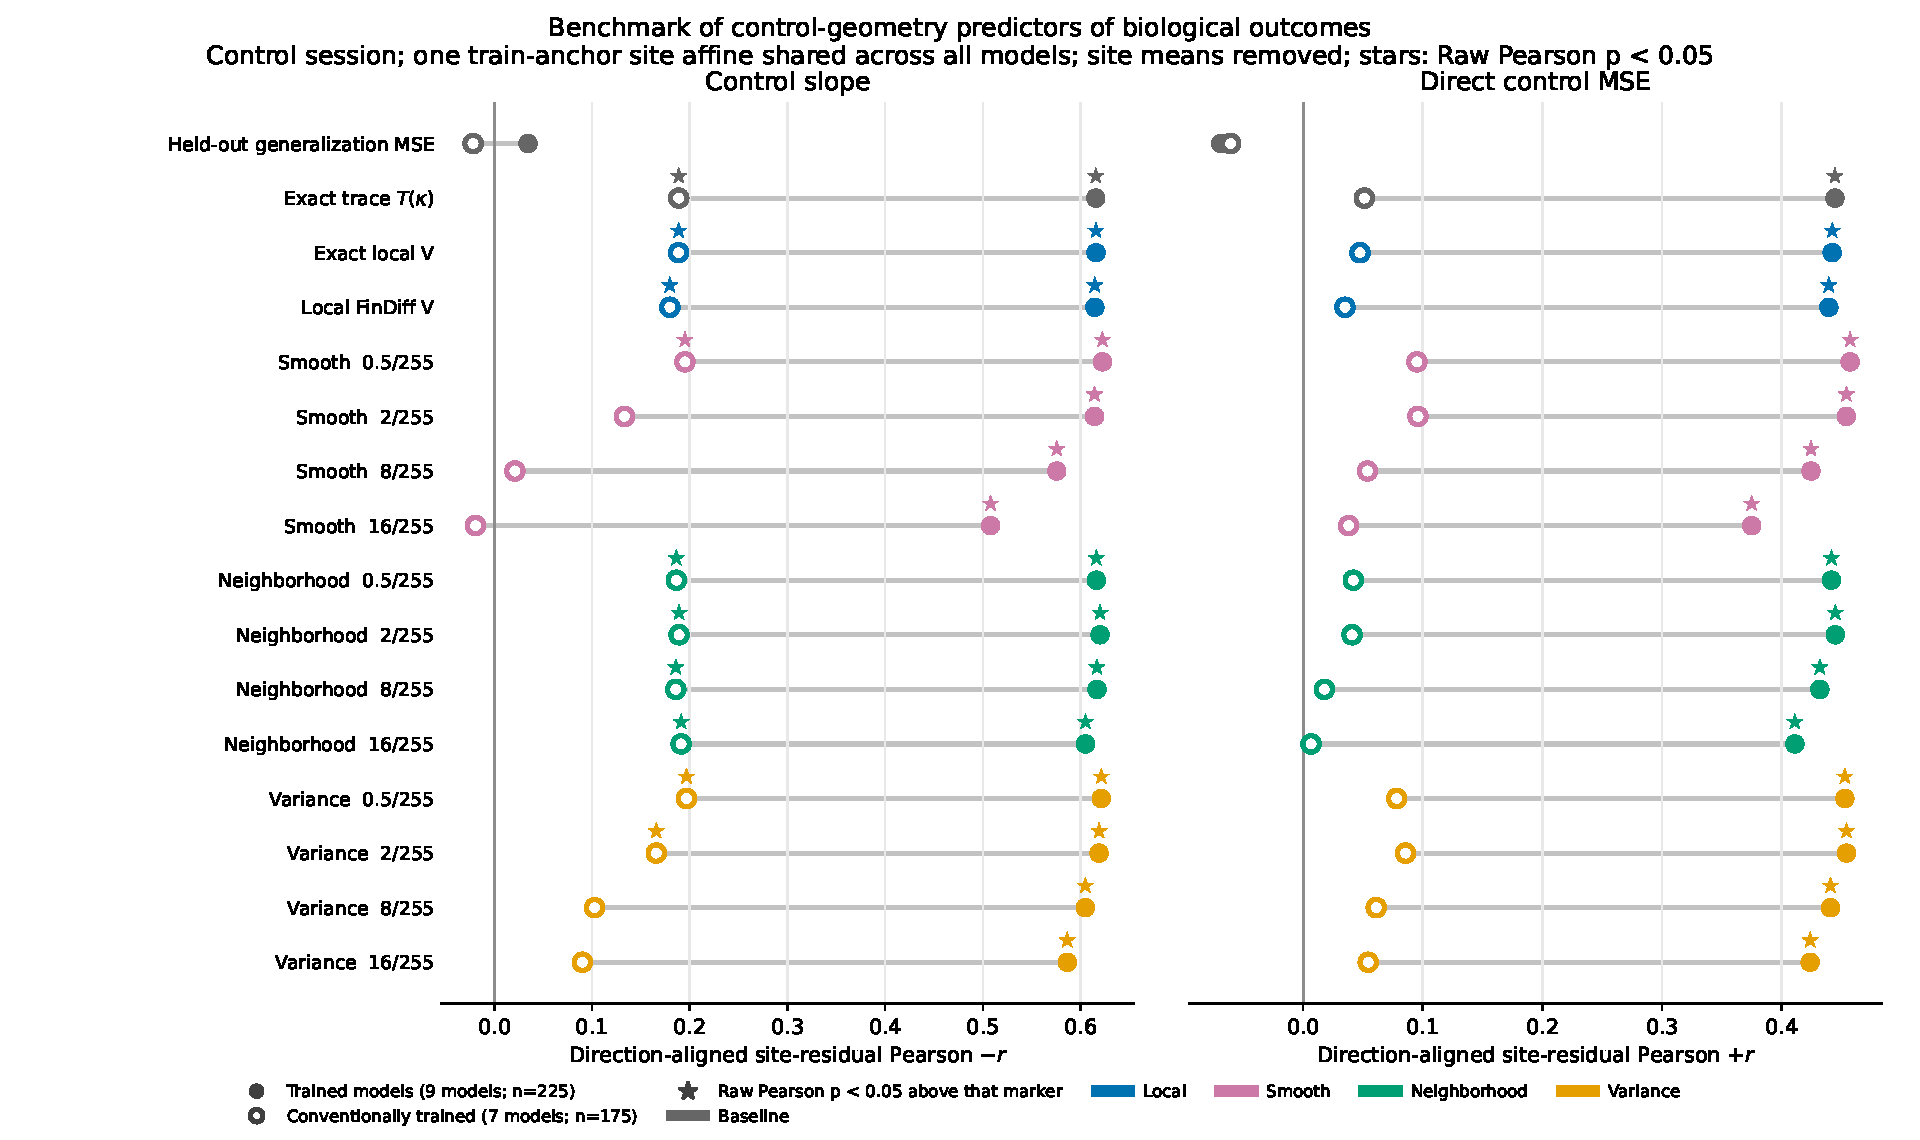
\includegraphics[width=0.44\linewidth,height=0.22\textheight,keepaspectratio]{figures/nonlinear_control_biological_validation.pdf}\\[2pt]
    % 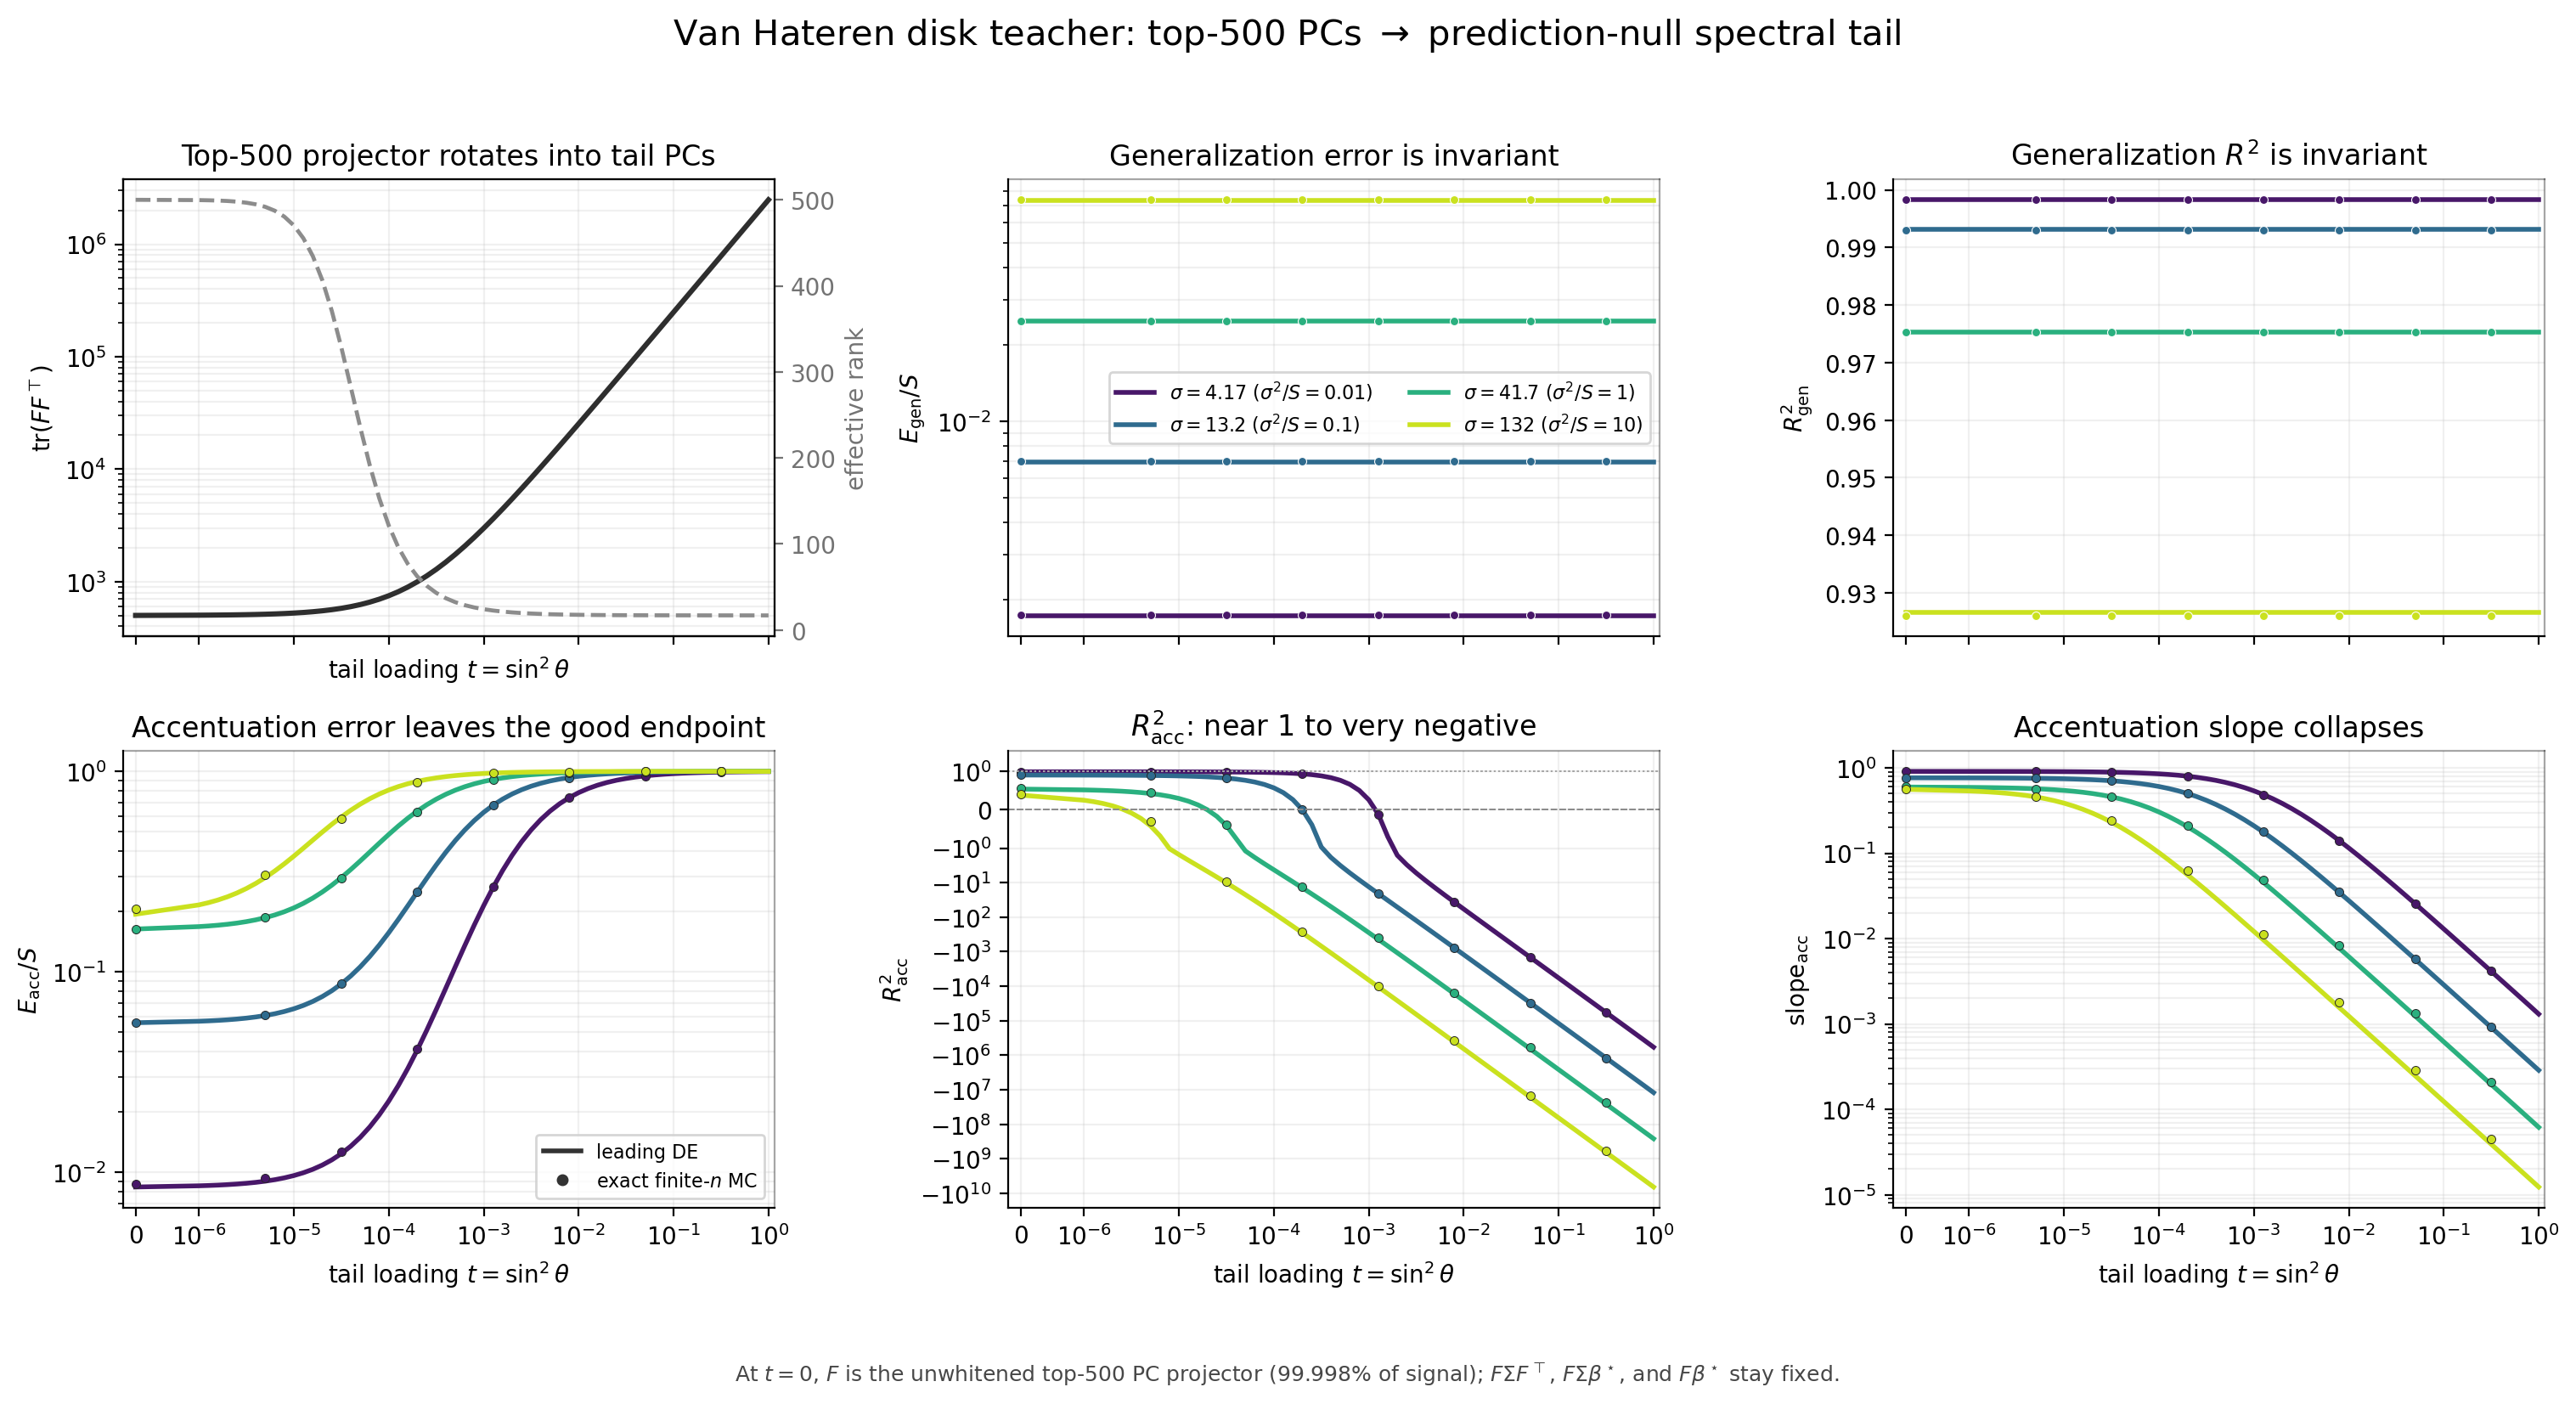
\includegraphics[width=0.45\linewidth,height=0.2\textheight,keepaspectratio]{figures/VanHateren_Top500PC_prediction_null_feature_rotation.png}
    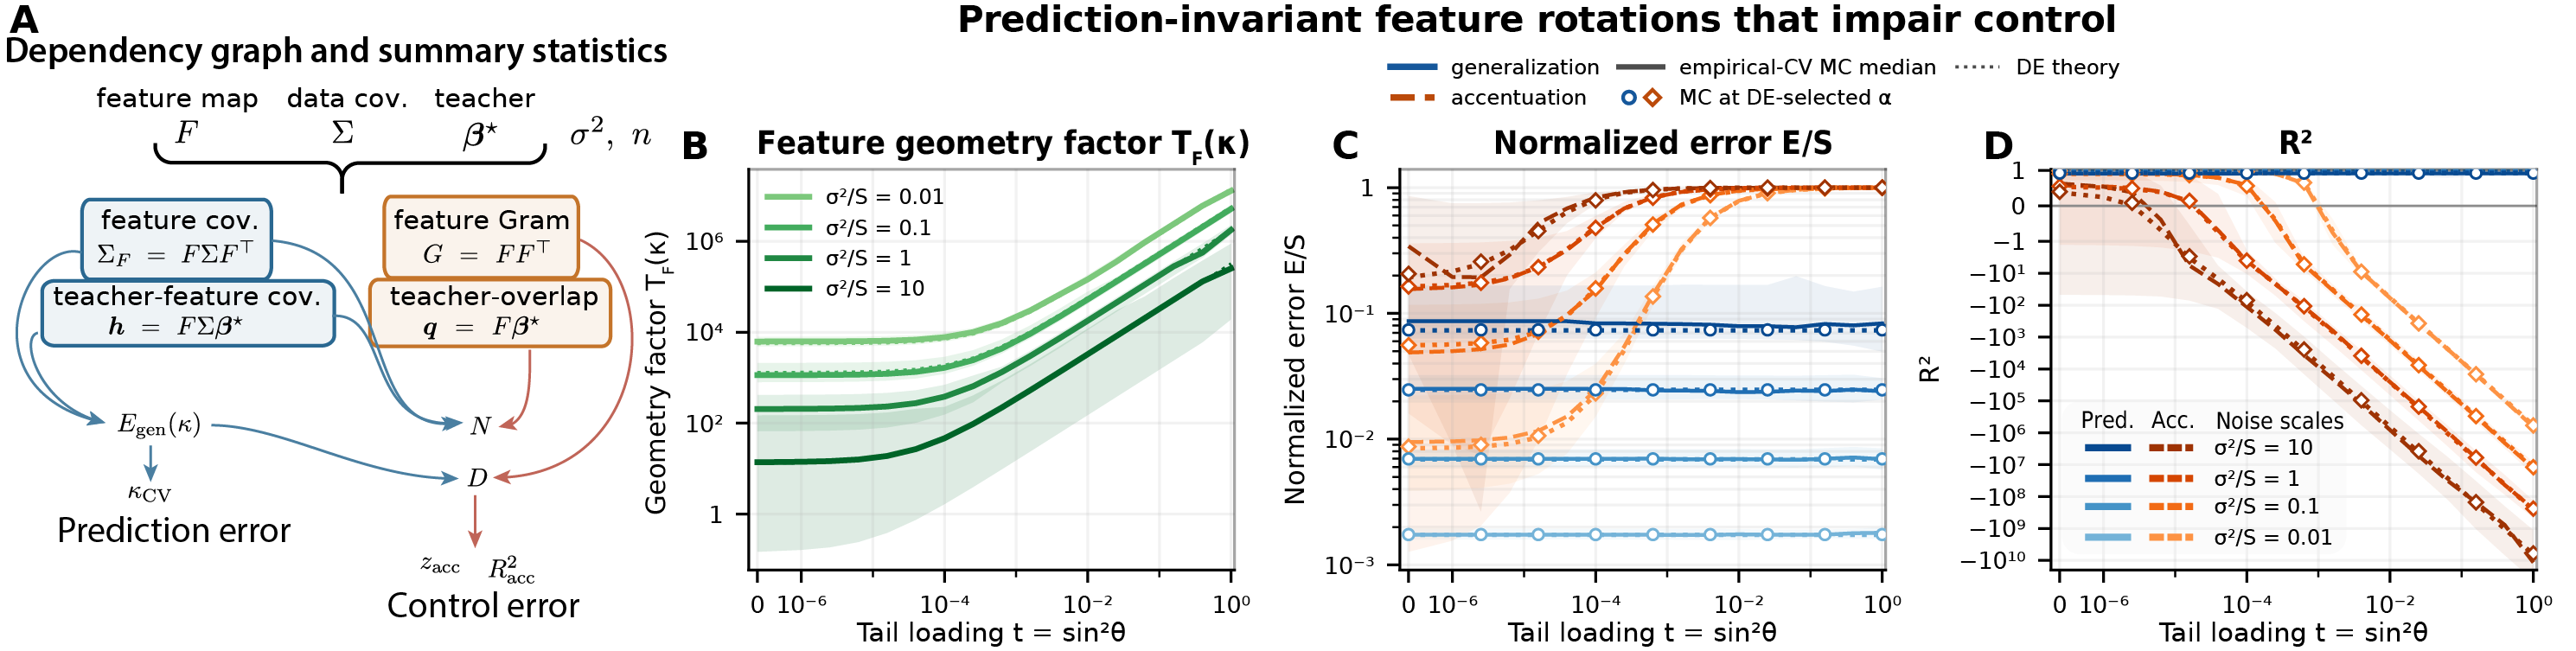
\includegraphics[width=\linewidth]{figures/Figure_linear_feature_gauge.png}
    \vspace{-15pt}
    \caption{\textbf{Feature geometry decides control.}
    \textbf{A}~Dependency graph: $(\Sigma_F,F\Sigma\bstar,S,\sigma^2,n)$ fix generalization and the cross-validated penalty; control additionally needs $\GramDef$ and $F\bstar$ (full graph: Fig.~\ref{fig:summary_stats_dep_graph}).
    \textbf{B-D}~For van Hateren images, rotating the top-500-PC projector feature into the spectral tail: $E_{gen}$ and $R^2_{gen}$ are invariant while $R^2_{acc}$ and the slope collapse; DE (lines) matches Gaussian-design Monte Carlo (markers). Construction: App.~\ref{sec:app-methods-feature}; further rotations: App.~\ref{sec:app-ext-gauge}. }
    %\textbf{C}~Neuronal data: site-demeaned association of each candidate predictor with biological control slope (left) and control error (right) across nine trained (filled) and seven conventionally trained (open) models. Held-out error carries no model-order information; the exact trace, $V_\phi$ and its neighborhood versions do. (Draft: keep 5 rows.)}
    \label{fig:feature}%\label{fig:nonlinear-biological-validation}
\end{figure}
\vspace{-8pt}
\section{Linear feature ridge: effect of gradient geometry} %the map decides what reaches the gradient
\label{sec:feature}

Pixel regression explains why one student fails; it cannot explain why ten equally predictive backbones fail differently. We idealize a backbone as a fixed linear map $F\in\R^{p\times d}$, fit $\hat w$ by ridge on features $F\x$, and accentuate along the pixel gradient $\bhat=F^\top\hat w$. Let $\Sigma_F:=F\Sigma F^\top$ be the feature covariance and $\GramDef$ the Euclidean feature Gram. The best realizable feature weight and its irreducible error are $w^\star=\Sigma_F^\dagger F\Sigma\bstar$ and $S_\perp=S-{w^\star}^\top \Sigma_F w^\star$ (App.~\ref{lem:mr-feature-weights}).

% \begin{prop}[Feature ridge: prediction and control]\label{prop:feature-de}\label{prop:linfeat_acc_ND}\label{prop:linfeat_gen_err}
% With $\kappa$, $B^F$ and $\mathrm{df}^F$ built from $(\Sigma_F,w^\star)$ and aspect ratio $p/n$, the mean fitted pixel weight is the realizable weight shrunk in feature space and back-projected, and the norm inflation carries a map-dependent \emph{gradient-geometry factor} $T_F$:
% \begin{equation}
% \bar\beta_{F,\kappa}:=F^\top(\Sigma_F+\kappa I)^{-1}F\Sigma\bstar,
% \quad
% % V_F(\kappa):=\frac{E_{gen,DE}+\sigma^2}{n}\,T_F(\kappa),
% % \,
% % T_F(\kappa):=\operatorname{Tr}\big[\Gram(\Sigma_F+\kappa I)^{-2}\Sigma_F\big].
% V_F(\kappa):=\frac1n(E_{gen,DE}+\sigma^2)\,\underbrace{\operatorname{Tr}\big[\Gram(\Sigma_F+\kappa I)^{-2}\Sigma_F\big]}_{T_F(\kappa):=},
% \label{eq:feature-mean-variance}
% \end{equation}
% Then
% \begin{equation}
% E_{gen,DE}=\frac{n(\kappa^2B^F_{1,2}+S_\perp+\sigma^2)}{n-\mathrm{df}^F_2}-\sigma^2,
% \qquad
% N_{DE}={\bstar}^\top\bar\beta_{F,\kappa},
% \qquad
% D_{DE}=\|\bar\beta_{F,\kappa}\|^2+V_F(\kappa).
% \label{eq:feature-de}
% \end{equation}
% Setting $F=I$ gives $\bar\beta_{F,\kappa}=\bar\beta_\kappa$ and $T_F=\mathrm{df}_{1,2}$, recovering Prop.~\ref{prop:pixel-de}. (Proofs: App.~\ref{sec:app-feature-regression}.)
% \end{prop}
\begin{prop}[Feature ridge: prediction and control]\label{prop:feature-de}\label{prop:linfeat_acc_ND}\label{prop:linfeat_gen_err}
With $\kappa$, $B^F$ and $\mathrm{df}^F$ built from $(\Sigma_F,w^\star)$ and aspect ratio $p/n$,
\begin{equation}\small
E_{gen,DE}=\frac{n(\kappa^2B^F_{1,2}+S_\perp+\sigma^2)}{n-\mathrm{df}^F_2}-\sigma^2,
\qquad
N_{DE}={\bstar}^\top\bar\beta_{F,\kappa},
\qquad
D_{DE}=\|\bar\beta_{F,\kappa}\|^2+V_F(\kappa).
\label{eq:feature-de}
\end{equation}
where
the mean fitted pixel weight $\bar\beta_{F,\kappa}$ is the realizable weight shrunk in feature space and back-projected, and the norm inflation carries a map-dependent \emph{gradient-geometry factor} $T_F$:
\begin{equation}\small
\bar\beta_{F,\kappa}:=F^\top(\Sigma_F+\kappa I)^{-1}F\Sigma\bstar,
\quad
% V_F(\kappa):=\frac{E_{gen,DE}+\sigma^2}{n}\,T_F(\kappa),
% \,
% T_F(\kappa):=\operatorname{Tr}\big[\Gram(\Sigma_F+\kappa I)^{-2}\Sigma_F\big].
V_F(\kappa):=\frac1n(E_{gen,DE}+\sigma^2)\,\underbrace{\operatorname{Tr}\big[\Gram(\Sigma_F+\kappa I)^{-2}\Sigma_F\big]}_{T_F(\kappa):=},
\label{eq:feature-mean-variance}
\end{equation}
Setting $F=I$ gives $\bar\beta_{F,\kappa}=\bar\beta_\kappa$ and $T_F=\mathrm{df}_{1,2}$, recovering Prop.~\ref{prop:pixel-de}. (Proofs: App.~\ref{sec:app-feature-regression}.)
\end{prop}
The structure is the same as in pixel ridge, so the interpretation carries over: $N$ is the teacher's alignment with the mean weight, $D$ is that weight's norm plus an inflation, and the unrealizable signal $S_\perp$ simply acts as extra response noise. What changes is what determines the two objects. Prediction sees the feature map only through $\Sigma_F$ and $F\Sigma\bstar$: the whole curve $E_{gen,DE}(\kappa)$, hence the cross-validated $\kappa$ and $R^2_{gen}$, is a function of $(\Sigma_F,F\Sigma\bstar,S,\sigma^2,n)$. Control additionally depends on the Gram $\Gram$ and on the teacher overlap $F\bstar$, (Fig.~\ref{fig:feature}\textbf{A}; Cor.~\ref{cor:mr-summary-statistics}). Thus the statistics governing control generically exceed those governing prediction. They coincide only in special cases, for instance white data $\Sigma=I$, where $\Gram=\Sigma_F$ and $F\bstar=F\Sigma\bstar$ (App.~\ref{sec:app-gauge-fragility}).
This extra degree of freedom can be seen clearly through the group that transforms feature map without affecting prediction.
\begin{prop}[Prediction-preserving gauge]\label{prop:gauge}
For $\Sigma\succ0$ and any orthogonal $Q$ with $Q\Sigma^{1/2}\bstar=\Sigma^{1/2}\bstar$, the map $F\mapsto F\Sigma^{1/2}Q\Sigma^{-1/2}$ preserves $\Sigma_F$ and $F\Sigma\bstar$, hence the joint feature--response covariance, $E_{gen,DE}(\kappa)$ and the DE-based prediction-optimal penalty $\kappa^\star_{gen}$, while changing $\Gram$ and $F\bstar$ and therefore control (Prop.~\ref{prop:mr-gauge}; construction in App.~\ref{sec:app-gauge-fragility}).
\end{prop}
Note, the gauge acts nontrivially on control only when the input is anisotropic: in white data, control error is also invariant to this group.
Variation of accentuation error grows with anisotropy. Rotating within it moves feature energy from high-variance to low-variance pixel directions at no cost to prediction (Fig.~\ref{fig:feature}B): along a continuous path, $E_{gen}$, $R^2_{gen}$ and the selected penalty are exactly constant, while $\operatorname{Tr}(FF^\top)$ grows by four orders of magnitude and $R^2_{acc}$ falls from near one to $-10^{8}$.
%\red{Random draws from the \textit{rotation group} span a huge range (Fig.~\ref{fig:supp-null-random}), so a population of equally predictive backbones with widely different control is the generic situation, not a construction.}

% For white data, the accentuation error is also invariant across this gauge group, leading to no dissociation.

\paragraph{What makes a map fragile.}
The response-independent part of $V_F$ is the geometric factor $T_F$, which has the spectral form
\begin{equation}
T_F(\kappa)=\sum_{k:s_k>0}\Big(\frac{s_k}{s_k+\kappa}\Big)^2\frac{\|g_k\|^2}{g_k^\top\Sigma g_k},
\qquad g_k:=F^\top v_k,
\label{eq:TF}
\end{equation}
with $(s_k,v_k)$ the eigenpairs of $\Sigma_F$ (Prop.~\ref{prop:mr-fragility}). It averages, over the feature PCs that survive ridge shrinkage ($s_k^2/(s_k+\kappa)^2\sim1$), the ratio between the Euclidean energy of the backpropagated PC gradient $\|g_k\|^2$ and its energy under the natural-image covariance $g_k^\top\Sigma g_k$. Thus, a map is fragile when its \textit{well-resolved feature directions backpropagate into low-variance, high-spatial-frequency pixel directions}. This is the linear counterpart of the third observation of Sec.~\ref{sec:phenomena}, and it can be computed from the map and the image statistics alone.

% \paragraph{Summary: When is control fragile although prediction is fine?}
% Holding the prediction error fixed, the leading control error (Eqs.~\ref{eq:pixel-de}, \ref{eq:pixel-zacc-cv}, \ref{eq:feature-de}) grows with three separable factors:
% \textbf{(i) noise} $(E_{gen}+\sigma^2)/n$, the estimation-noise level, which is the only factor visible from held-out accuracy;
% \textbf{(ii) spectrum} the mismatch between prediction-optimal and control-optimal penalties, Eq.~\ref{eq:pixel-zacc-cv}, which is zero for white data and grows with anisotropy and with teacher energy in low-variance modes;
% \textbf{(iii) map} $T_F$, the ridge-weighted ratio of Euclidean to natural-covariance gradient energy, a property of the feature map alone.
% Visual neuronal responses are known to be highly noisy \citep{goris2014partitioning,churchland2010stimulus}, meeting (i);
% Natural images make (ii) large for every model; the feature map decides (iii), and equally predictive maps can differ in it without bound.
\paragraph{Summary: When is control fragile although prediction is fine?}
Control fails when the norm inflation $V_F$ overshoots the shrinkage deficit (Eqs.~\ref{eq:pixel-de},~\ref{eq:feature-de}). 
The inflation $V_F=(E_{gen}+\sigma^2)\,T_F(\kappa)/n$ is a product of three factors, 
\textbf{(i) response noise} $E_{gen}+\sigma^2$;
\textbf{(ii) limited data} $1/n$;
\textbf{(iii) gradient geometry} $T_F$, the ratio of Euclidean to covariance-weighted gradient energy, a property of the feature map;
\textbf{(iv) mismatched regularization}: on anisotropic data, the cross-validated penalty is designed for prediction, but not control-optimal and can leave a large control error  (Eq.~\ref{eq:pixel-zacc-cv}).
Held-out accuracy reflects only (i); (iii) and (iv) are invisible to it. Neuronal recordings are noisy and short \citep{goris2014partitioning,churchland2010stimulus}, supplying (i)--(ii); natural images make (iv) large for every model; and the feature map decides (iii), in which equally predictive maps differ without bound.


\begin{figure}[t]
    \centering
    \vspace{-15pt}
    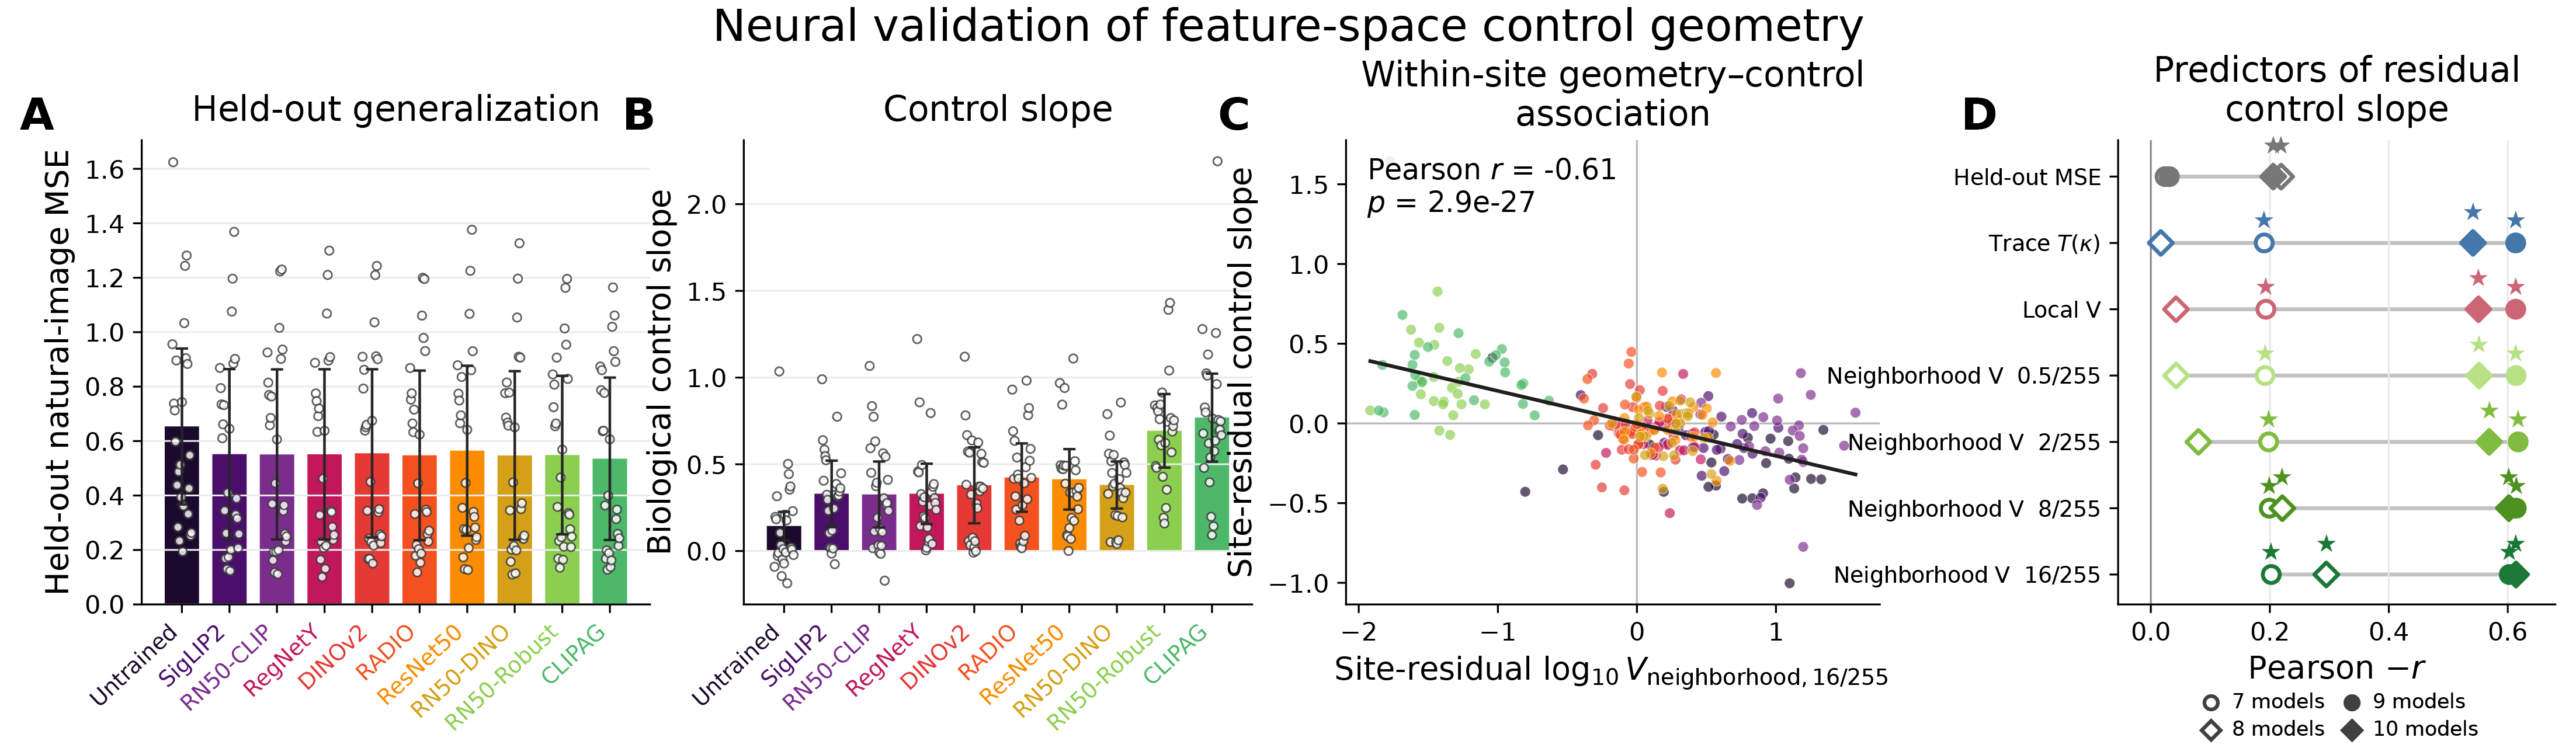
\includegraphics[width=\linewidth]{figures/Figure_nonlinear_neuro_diagnostic.png}
    \vspace{-18pt}
    \caption{\textbf{Gradient-feature geometry in nonlinear model predicts biological control across encoding models.}
% We evaluated ten encoding models at 25 neural recording sites from five subjects. Control-session responses were aligned to the encoding-session scale using a site-specific affine map fitted only on repeated natural-image anchors and shared across models.
% We reproduced the results using published preprocessed data from \citetPW.
% \textbf{A}~MSE on held-out natural-image in the control session, analogous to $E_{\mathrm{val}}\approx E_{\mathrm{gen}}+\sigma^2$.
% \textbf{B}~Control slope between \textit{in vivo} measured and model-predicted neural responses to accentuated stimuli. In \textbf{A,B}, bars show the mean across 25 sites, dots show individual sites, and error bars denote $\pm1$ SE across sites.
% \textbf{C}~Raw $\log_{10}V_\phi$ computed from Jacobian energy averaged over a $16/255$ neighborhood is anticorrelated with control slope after removing each site's ten-model mean (Pearson $r=-0.56$ across 250 site--model pairs).
% \textbf{D}~Pearson correlation ($-r$) between site-centered control slope and seven raw $\log_{10}$ predictors: held-out MSE, the gradient-geometry trace $T_\phi(\kappa)$, exact-local $V_\phi$, and neighborhood $V_\phi$ at four scales.
% Control slope was mean-subtracted within site using all ten models; predictors remained raw. Markers denote 10/9/8/7-model subsets (all / no untrained AlexNet / no robust models (CLIPAG,RN50-robust) / neither), and stars indicate raw two-sided Pearson $p<0.05$. All estimators and scales: App.~\ref{sec:app-ext-nonlinear}.
Published preprocessed data of \citetPW.
\textbf{A}~Held-out natural-image MSE in the control session ($E_{\mathrm{val}}\approx E_{\mathrm{gen}}+\sigma^2$).
\textbf{B}~Slope of observed-over-predicted responses to accentuated stimuli. \textbf{A,B}: mean over 25 sites (bars), sites (dots), $\pm1$ SE.
\textbf{C}~Raw $\log_{10}V_\phi$ ($16/255$ neighborhood) against control slope with each site's ten-model mean removed (Pearson $r=-0.56$, 250 site--model pairs).
\textbf{D}~Pearson $-r$ between site-centered control slope and seven raw $\log_{10}$ predictors (held-out MSE, $T_\phi(\kappa)$, exact-local and neighborhood $V_\phi$ at four scales) for 10/9/8/7-model subsets (all / no untrained AlexNet / no robust models / neither); stars: raw two-sided $p<0.05$. All estimators: App.~\ref{sec:app-ext-nonlinear}.} %without multiple-comparison correction
    \label{fig:nonlinear-biological-validation}
    \vspace{-8pt}
\end{figure}

\vspace{-7pt}
\section{Nonlinear feature ridge: a generalized diagnostic for DNN}
\label{sec:nonlinear}
% Prop.~\ref{prop:feature-de} shows
For linear feature,  $V_F$ is the main culprit of accentuation error. For nonlinear features $\phi$, is there an analogous quantity that preludes control failure?
Viewing a nonlinear feature map $\phi$ as locally linear, we use its Jacobian $J_\phi(x)$ to replace $F$ in Eq.~\ref{eq:TF},
% For a nonlinear feature map $\phi$ with Jacobian $J_\phi(x)$ and natural-image feature covariance eigenpairs $(s_k,v_k)$, replacing $F$ by the local Jacobian gives
\begin{equation}\small
T_\phi(x,\kappa)=\sum_k\frac{s_k}{(s_k+\kappa)^2}\,\|J_\phi(x)^\top v_k\|^2,
\qquad
V_\phi:=\frac{E_{val}}{n}\,\E_x\big[T_\phi(x,\kappa)\big],
\label{eq:Tphi}
\end{equation}
where $(s_k,v_k)$ is the eigenpairs of feature covariance on natural-images, and $J_\phi(x)^\top v_k=\nabla_x[v_k^\top\phi(x)]$ is the pixel gradient of feature PC $k$, obtainable by one backward pass per PC, and $V_\phi$ mirrors the norm inflation $V_F$ of Eq.~\ref{eq:feature-mean-variance} with $E_{val}\approx E_{gen}+\sigma^2$.
Since an accentuation path travels far from the seed, we also evaluate smoothed versions in which the Jacobian is averaged, or the squared gradient is averaged, over a Gaussian neighborhood of the seed at pixel-noise scales from $0.5/255$ to $16/255$ (App.~\ref{sec:app-nonlinear-diagnostic}).
% This is exact for linear $\phi$ and a theory-motivated diagnostic for nonlinear networks. %, where $s_k=g_k^\top\Sigma g_k$ no longer holds.
%For linear $\phi$ this is exact; for a network it is a diagnostic motivated by the theory, because the identity $s_k=g_k^\top\Sigma g_k$ that made $T_F$ a ratio of gradient energies no longer holds.

We computed these quantities for all 250 site--model pairs (App.~\ref{sec:app-methods-nonlinear}), with $\kappa$ set by each model's cross-validated penalty and feature spectrum, average over the ten seed images, and $E_{val}$ the held-out error of the control session. Because sites differ greatly in controllability, {we subtract each site's mean from the control outcome and correlate this residual with the predictors in log10 (Pearson $r$; Fig.~\ref{fig:nonlinear-biological-validation}\textbf{C,D})}. Held-out error carries essentially no ordering information ({$r=0.02$} with control slope, {$-0.04$} with control error, across the nine trained models), whereas exact-local $V_\phi$ reaches {$r=-0.58$ and $+0.40$}; the trace $T_\phi$ alone does {as well ($-0.61$, $+0.43$)}, so the ordering mainly comes from gradient geometry. Among the seven conventionally trained models the slope association is weaker but same-signed ({$r\approx-0.15$ to $-0.17$}): the two adversarially trained models are the strongest controllers and have by far the smallest $T_\phi$. {Neighborhood smoothing ($16/255$) keeps more of the ordering without the robust models ($r=-0.25$ vs.\ $-0.05$ for exact-local $V_\phi$ over eight models).} Thus, the gradient-geometry factor of linear feature maps carries over to deep networks, ranking equally predictive encoding models by \textit{in vivo} control where held-out accuracy cannot. %; the rankings are descriptive, not predictions of absolute control error.% (models repeated within sites)  .

\vspace{-7pt}
\section{Discussion}
\label{sec:discussion}
\vspace{-9pt}
A single mechanism accounts for the three neuronal phenomena: prediction measures weight error in the covariance metric, control measures it along the model's own gradient. In the linear theory the control error at fixed prediction error is governed by the three factors: noise, spectrum, and map, of which only the first is visible from held-out accuracy.
The practical implication is that selecting encoding models or penalties by held-out prediction cannot certify gradient-based control; validation must constrain the gradient, for instance through $T_\phi$, or test generated stimuli directly. The high-frequency artifacts of failed accentuations are not a cosmetic defect but the expected signature of low-variance directions that natural images never constrained.

\paragraph{Limitations.}
The theory assumes Gaussian inputs, a linear teacher, a fixed linear feature map and a linear accentuation path from a centered seed, while some phenomena (e.g. non-trivial Pearson r) requires multiple non-centered seeds.
The details of accentuation procedure (e.g. preconditioning and image prior) could be built in as natural extensions.
The leading DEs predict typical fits and the location of the control optimum but not the fluctuation-dominated error at that optimum (App.~\ref{sec:app-ratio-corrections}).
Our theory did not prove the relation between the diagnostic and control error for nonlinear features; its biological validation is descriptive. %Extending the deterministic equivalents to learned nonlinear features and to curved accentuation trajectories is the natural next step.

\clearpage
\section{Reproducibility Statement}
The theory assumptions, derivations, and deterministic equivalents are stated in the main text, with full derivations in the appendix. The code repository (will be released after camera ready) contains the core RMT library, CPU and GPU Monte Carlo scripts, notebooks recreating the figures, and saved outputs for the experiments shown here.

\section{Ethics Statement}
This work is theoretical and uses synthetic simulations, natural-image covariance spectra, and previously published neuronal recordings for validation. It does not introduce a deployed model, collect human-subject data, or release a dataset with personal information.


\section*{AI Use Statement}
{OpenAI ChatGPT, Codex and Anthropic Claude, including Claude Code, were used as general-purpose research, coding, and writing assistants throughout this work. 
The theory was developed iteratively between the authors and these systems. In some instances, the authors first derived a result and used an AI system to check the algebra, simplify the equations, or identify alternative interpretations; in others, an AI system proposed a derivation, simplification, or reading that the authors subsequently checked, corrected, and refined. The final conceptual synthesis emerged through this iterative process, while the authors determined the research questions, selected the scientific directions, and made all final decisions about the claims. The systems also assisted with designing, generating, debugging, profiling, executing, and documenting computational experiments and figure-generation code, as well as organizing, drafting, editing, and typesetting the manuscript. The authors reviewed all retained derivations and prose, inspected the code, validated numerical results against theory and direct computation, and checked the supporting references. The authors take full responsibility for the accuracy and integrity of the paper. No AI system is listed as an author.}
\bibliography{iclr2026/accentuation_rmt_iclr2026}
\bibliographystyle{iclr2026/iclr2026_conference}

\clearpage
\appendix
\tableofcontents{}
% \input{theory_appendix.tex}
% ---------------------------------------------------------------------------
% Appendix A: Extended results (supplementary figures).
% Order of the appendix: A extended results -> B detailed methods
% (extended_methods.tex) -> theory (theory_appendix_polished.tex).
% Plan and figure sources: notes/appendix_outline_plan.md.
% Figures not yet exported to figures/ are shown as \suppfigplaceholder boxes
% naming their source in the code repository (AccentuationPredRMT).
% ---------------------------------------------------------------------------

\providecommand{\suppfigplaceholder}[2][0.22\textheight]{%
  \fbox{\parbox[c][#1][c]{0.95\linewidth}{\centering\small
  \textcolor{magenta}{\textbf{[figure to insert]}}\\[2pt]
  \texttt{\detokenize{#2}}}}}

\section{Extended results}
\label{sec:app-extended-results}

The appendix has three parts.  This section collects supplementary figures
that extend the main-text figures.  Section~\ref{sec:app-methods} describes
the numerical experiments and the neuronal analyses in detail.  The theory
follows from Section~\ref{sec:app-theory-roadmap} on: every result stated in
derivation order, then proofs grouped by topic.

% ---------------------------------------------------------------------------
\subsection{Geometry of the ridge path}
\label{sec:app-ext-geometry}
% Supports Fig.~\ref{fig:geometry} (Sec.~\ref{sec:setup}) and the ridge-path
% paragraph of Sec.~\ref{sec:pixel}.  Theory: Prop.~\ref{prop:mr-iso-geometry},
% Exp.~\ref{ex:mr-dissociation}.  Methods: App.~\ref{sec:app-methods-geometry}.
\todo{One paragraph: exact conditional Gaussian of $\bhat\mid X$ in the plane of
a high- and a low-variance PC; (a) varying $\sigma^2$ at fixed $\lambda$,
(b) varying $\lambda$ at fixed $\sigma^2$; prediction-stationary point vs.\
$z=0$ crossing.}

\begin{figure}[ht]
\centering
\suppfigplaceholder{figures/geometry/ridge_paths_iso_error_geometry.pdf  (fix literal "68\%" in legend, overlapping teacher label)}
\caption{\textbf{Exact conditional geometry of ridge estimators in two
dimensions.} \todo{caption} Setting in App.~\ref{sec:app-methods-geometry}.}
\label{fig:supp-ridge-path-geometry}
\end{figure}

% ---------------------------------------------------------------------------
\subsection{Pixel-space ridge on natural images}
\label{sec:app-ext-pixel}
% Supports Fig.~\ref{fig:pixel} (Sec.~\ref{sec:pixel}).
% Methods: App.~\ref{sec:app-vanhateren-landscape-methods}.
% Theory: App.~\ref{sec:app-pixel-ridge}, \ref{sec:app-optimal-regularization},
% \ref{sec:app-ratio-corrections}.
\todo{Short text: (i) DE vs.\ natural-image Monte Carlo over the full
noise--regularization plane; (ii) slope landscapes; (iii) fixed penalty
vs.\ CV-selected vs.\ control-oracle penalty along the noise axis, including
where the leading DE fails (near the control optimum) and the Gaussian
surrogate of App.~\ref{sec:app-ratio-gaussian} takes over.}

\begin{figure}[ht]
\centering
\suppfigplaceholder{figures/vanhateren_landscape/export/composite/paper_composite_three_landscapes_de_mc_rows_figexport.pdf  (crop to the 2x3 heatmaps)}
\caption{\textbf{Deterministic equivalents versus natural-image Monte Carlo
for the landscapes of Fig.~\ref{fig:pixel}.} \todo{caption}}
\label{fig:supp-pixel-de-mc}
\end{figure}

\begin{figure}[ht]
\centering
\suppfigplaceholder{figures/vanhateren_landscape/landscape_slope_kappa.pdf}
\caption{\textbf{Slope landscapes} of generalization and accentuation, DE
(top) and Monte Carlo (bottom). \todo{caption}}
\label{fig:supp-pixel-slope}
\end{figure}

\begin{figure}[ht]
\centering
\suppfigplaceholder[0.3\textheight]{notebooks/outputs/pixel_ridge/vanhateren_selection_estimation/selection_vs_estimation_extended_with_sklearn_cv.pdf}
\caption{\textbf{Fixed, prediction-selected and control-selected penalties
along the noise axis.} \todo{caption; leading DE vs.\ Gaussian surrogate vs.\
MC; empirical LOOCV}}
\label{fig:supp-pixel-selection}
\end{figure}

% Q6 (decide later): synthetic isotropic / power-law validation of the
% generalization, accentuation and peer DEs (figures/peer_validation/
% r2_peer_validation.png; figures/model_selection/cv_selected_r2.png).
% \label{fig:supp-synthetic-validation}

% ---------------------------------------------------------------------------
\subsection{Linear feature ridge: the prediction-null family}
\label{sec:app-ext-gauge}
% Supports Fig.~\ref{fig:feature} (Sec.~\ref{sec:feature}).
% Theory: App.~\ref{sec:app-gauge-fragility} (Prop.~\ref{prop:app-feature-gauge},
% Cor.~\ref{cor:mr-rotation}); full dependency graph stays in theory as
% Fig.~\ref{fig:summary_stats_dep_graph}.  Methods: App.~\ref{sec:app-methods-feature}.
\todo{Short text: continuous rotation from top-$p$ PC projectors
(Fig.~\ref{fig:app-null-rotation}); random draws from the family
(Fig.~\ref{fig:supp-null-random}); what the rotation does to individual
feature rows (Fig.~\ref{fig:supp-null-row-spectra}); dependence on the
feature dimension $p$ (Fig.~\ref{fig:supp-null-dimension}).}

\begin{figure}[ht]
\centering
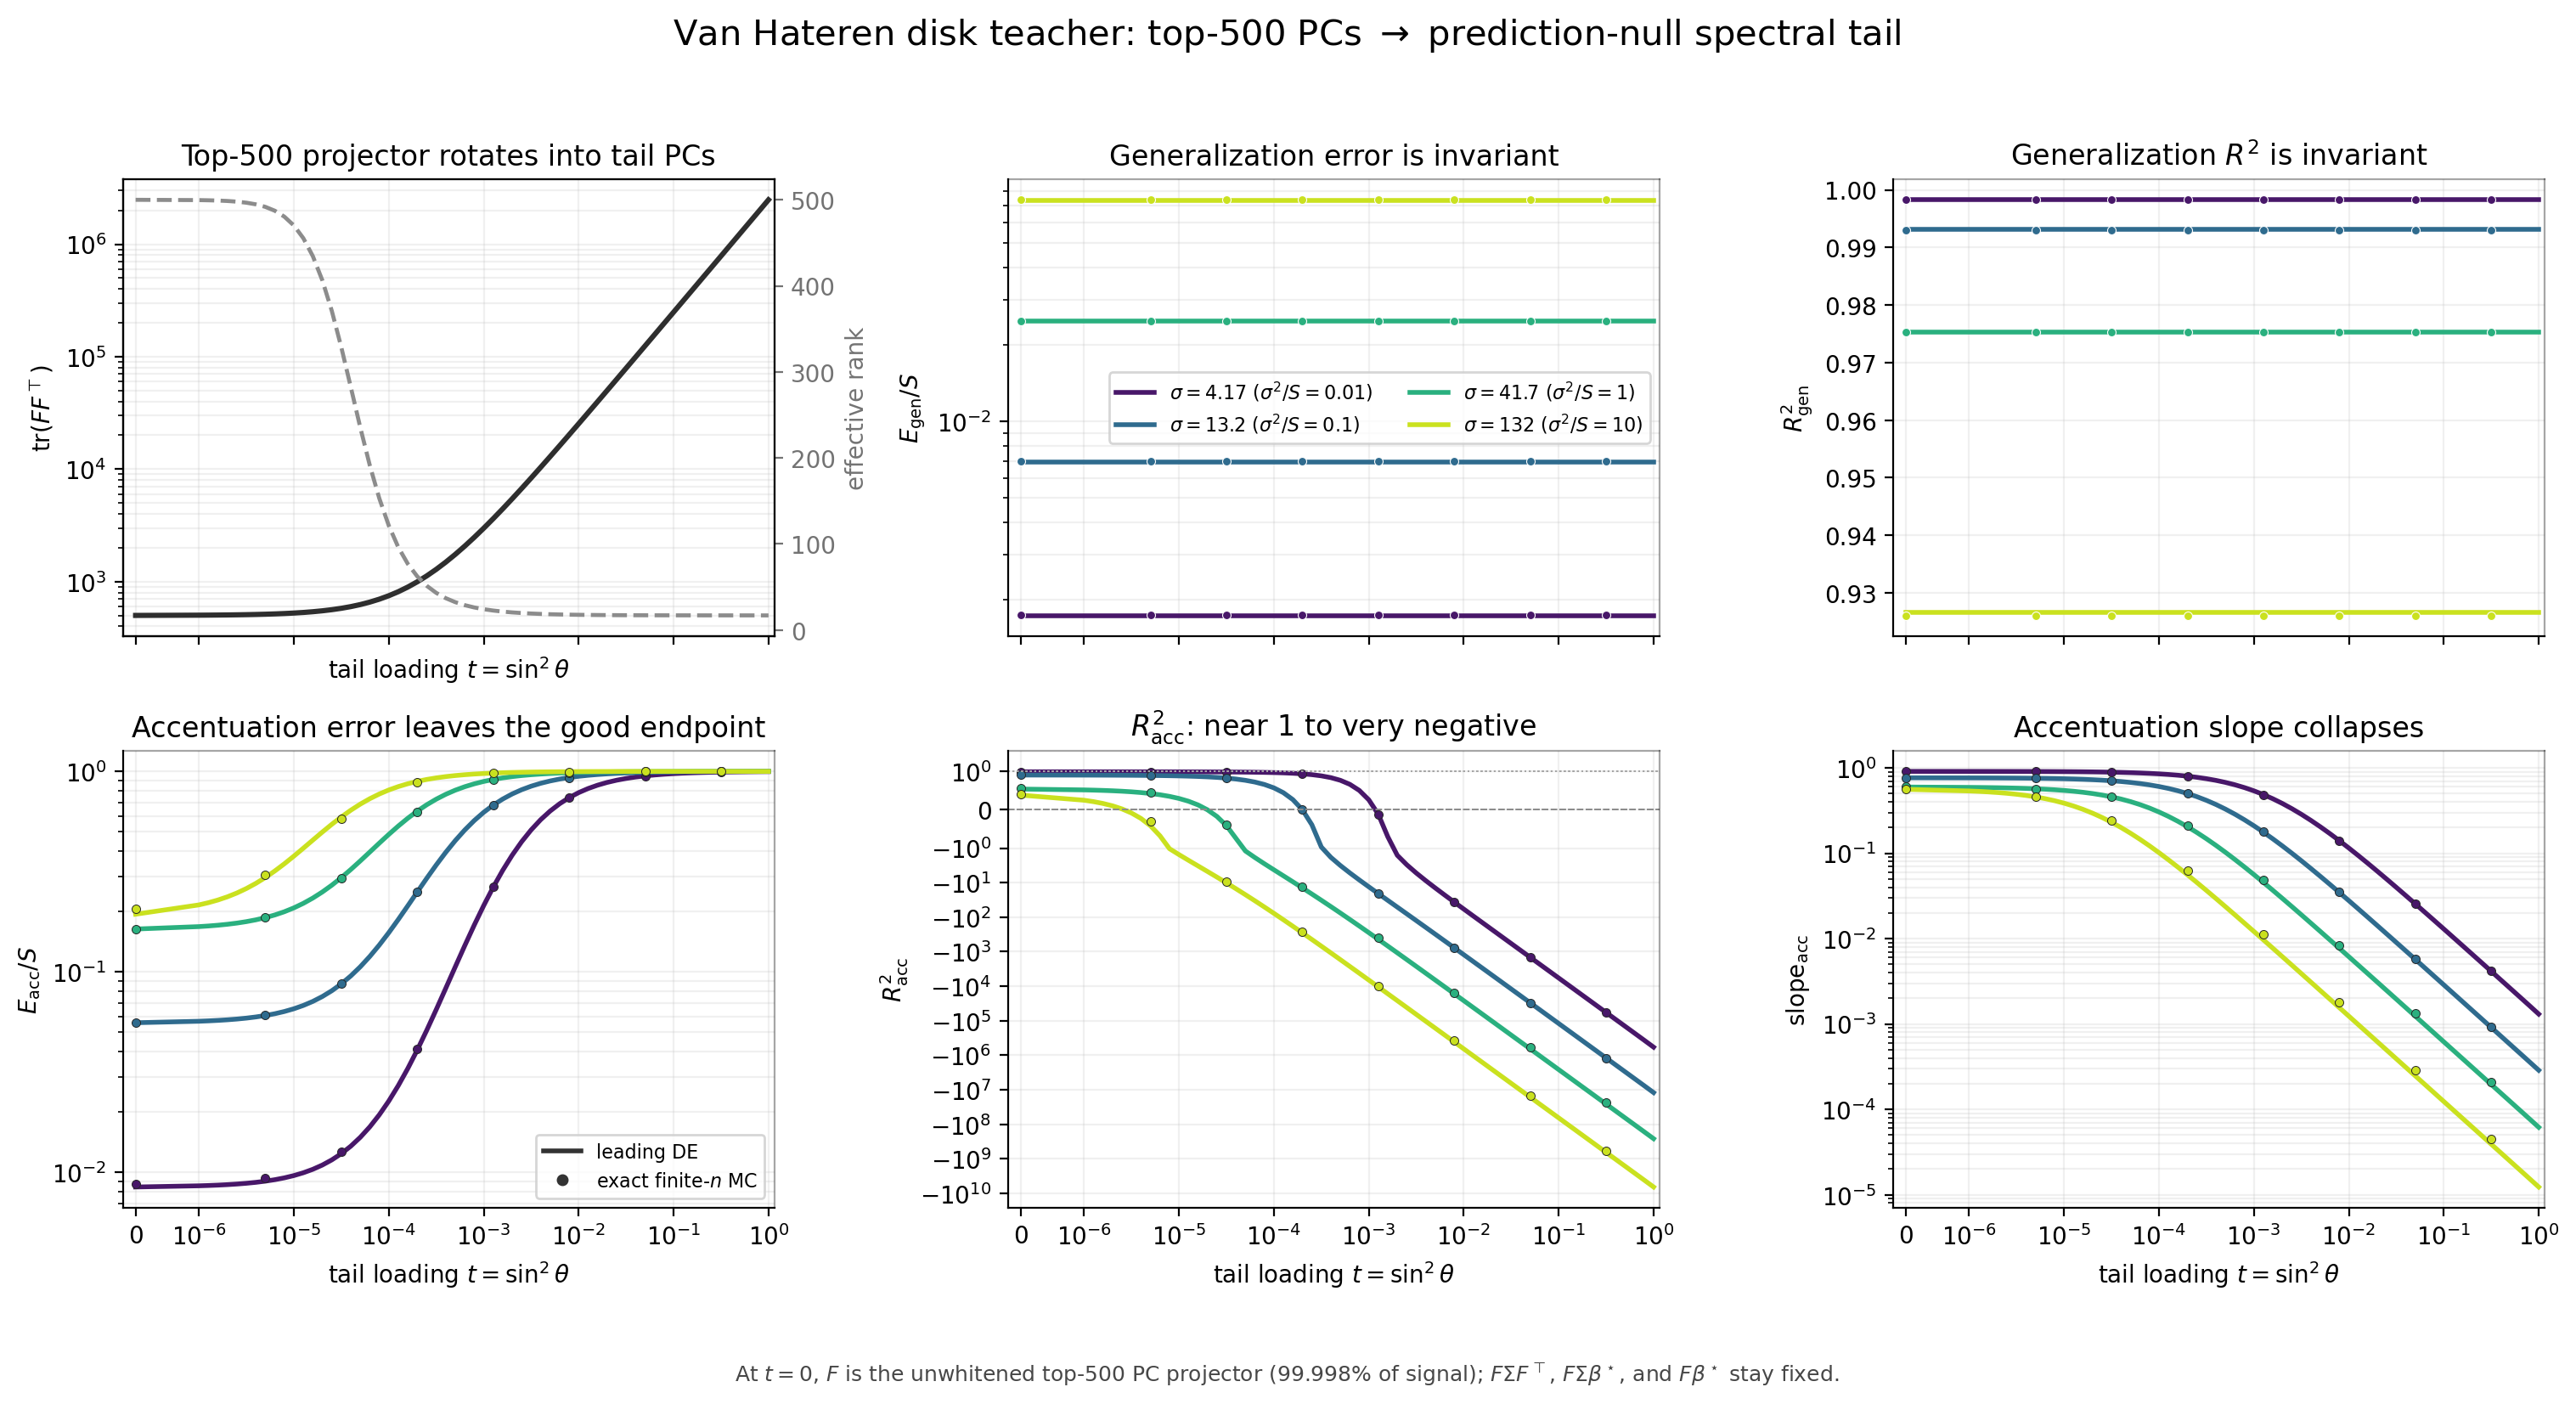
\includegraphics[width=1\linewidth]{figures/VanHateren_Top500PC_prediction_null_feature_rotation}\\
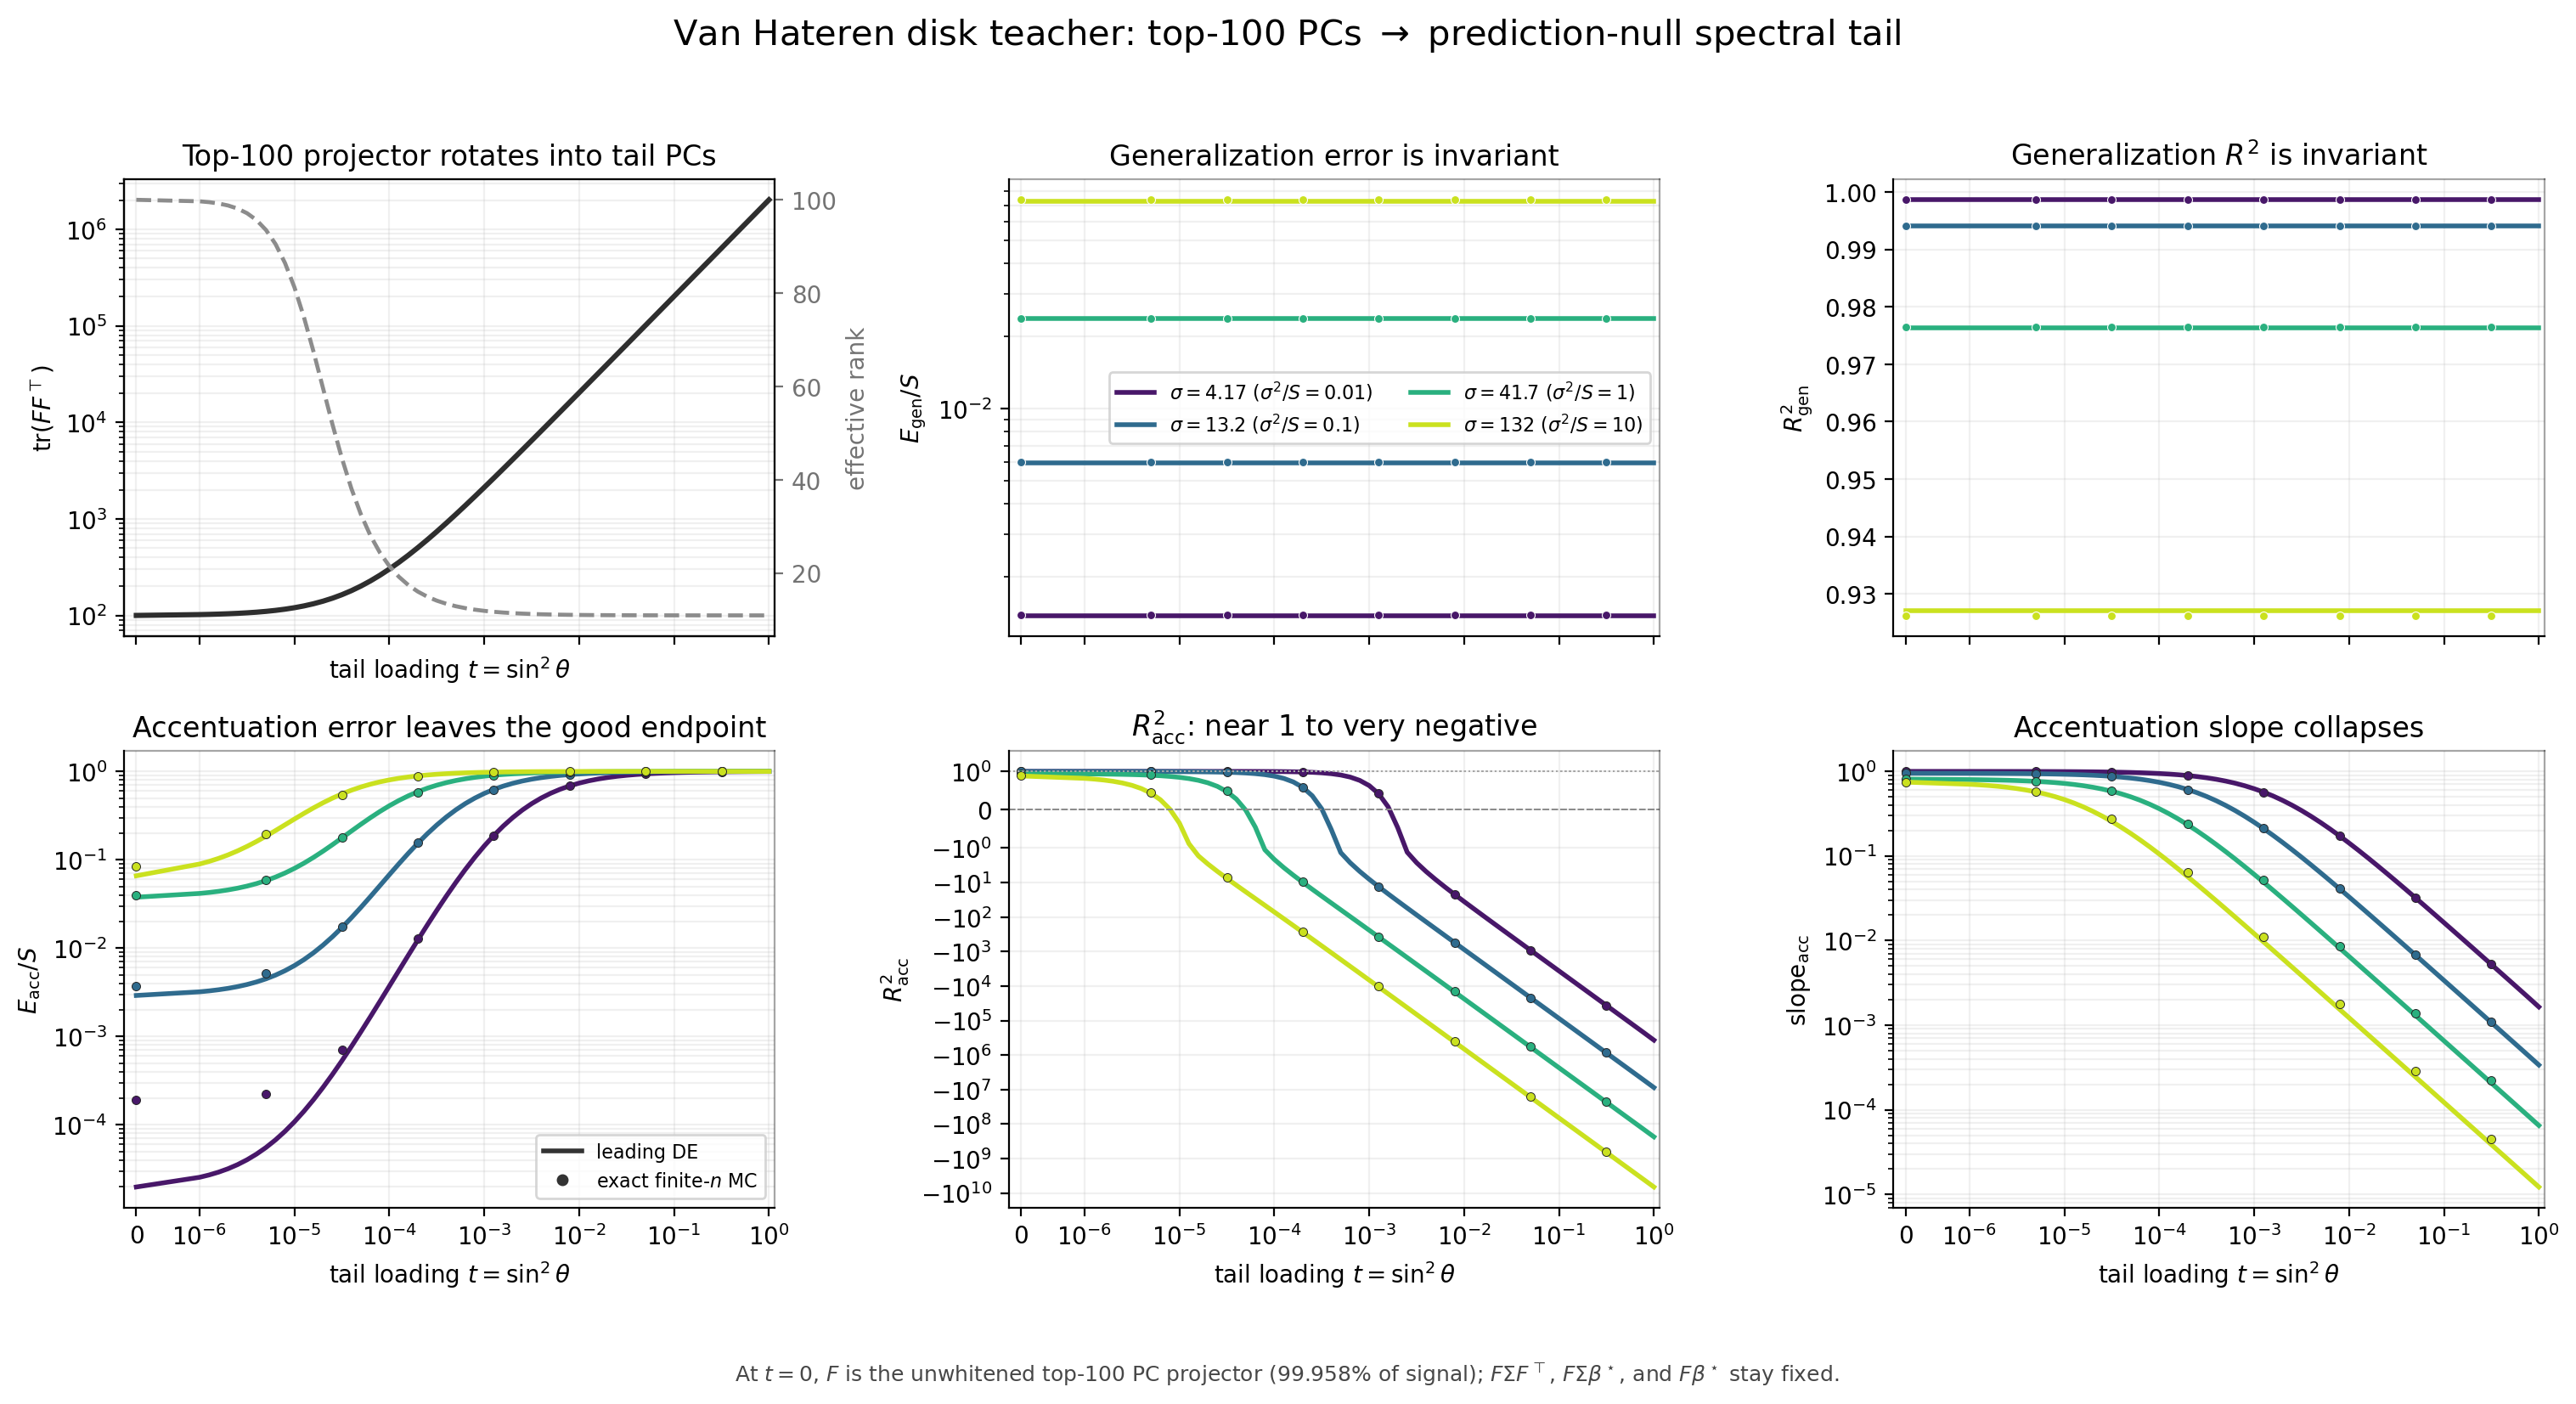
\includegraphics[width=1\linewidth]{figures/VanHateren_Top100PC_prediction_null_feature_rotation}
\caption{\textbf{Continuous prediction-null rotation on van Hateren images}
(Corollary~\ref{cor:mr-rotation}), starting from the top-500 (top) and
top-100 (bottom) PC projectors and rotating their null part into the
spectral tail.  Generalization error, $R^2_{gen}$ and the selected penalty are
exactly constant in the tail loading $t$, while $\operatorname{Tr}(FF^\top)$,
accentuation error, $R^2_{acc}$ and slope change by orders of magnitude.
Lines: leading DE; markers: finite-$n$ Monte Carlo.}
\label{fig:app-null-rotation}
\end{figure}

\begin{figure}[ht]
\centering
\suppfigplaceholder{figures/null_rotations/vanhateren_p500_random_null_diversity.pdf}
\caption{\textbf{Random maps from the prediction-null family ($p=500$).}
\todo{caption: identical $E_{gen}$, $R^2_{gen}$; accentuation metrics
spread over orders of magnitude with $\operatorname{Tr}(FF^\top)$.}}
\label{fig:supp-null-random}
\end{figure}

\begin{figure}[ht]
\centering
\suppfigplaceholder{figures/null_rotations/vanhateren_top_pc_tail_feature_spectra.pdf}
\caption{\textbf{Spectral location of individual feature rows along the
rotation.} \todo{caption}}
\label{fig:supp-null-row-spectra}
\end{figure}

\begin{figure}[ht]
\centering
\suppfigplaceholder{figures/null_rotations/vanhateren_null_dimension_curves.pdf}
\caption{\textbf{Null rotation across feature dimension $p$.} \todo{caption:
leading DE vs.\ Gaussian distributional DE vs.\ MC.}}
\label{fig:supp-null-dimension}
\end{figure}

% ---------------------------------------------------------------------------
\subsection{Peer review in the neuronal experiment}
\label{sec:app-ext-peer}
% Supports Sec.~\ref{sec:phenomena} (recognition without generation) and the
% peer-review paragraph of Sec.~\ref{sec:pixel}.  Theory:
% App.~\ref{sec:app-peer-review}, \ref{sec:app-peer-shared}.
% Methods: App.~\ref{sec:app-methods-peer}.
\todo{Short text: generator $\times$ reviewer matrices; self (diagonal) vs.\
peer (off-diagonal) distributions and tests.}

\begin{figure}[ht]
\centering
\suppfigplaceholder{figures/nonlinear_control/neural_peer_review/peer_review_four_metrics_jacob_order.pdf}
\caption{\textbf{Neuronal peer review.} Rows: generating model; columns:
reviewing model; diagonal: self-evaluation. \todo{caption}}
\label{fig:supp-neural-peer-matrix}
\end{figure}

\begin{figure}[ht]
\centering
\suppfigplaceholder{NEW: self vs peer R^2 and slope distributions (stats in tables/nonlinear_control/.../PEER_REVIEW_SELF_VS_PEER_RESULTS.md)}
\caption{\textbf{Self-evaluation versus peer review.} \todo{caption}}
\label{fig:supp-neural-self-vs-peer}
\end{figure}

% ---------------------------------------------------------------------------
\subsection{Nonlinear gradient diagnostic: full comparison}
\label{sec:app-ext-nonlinear}
% Supports Fig.~\ref{fig:nonlinear-biological-validation} (Sec.~\ref{sec:nonlinear}).
% Theory: App.~\ref{sec:app-nonlinear-diagnostic}.
% Methods: App.~\ref{sec:app-methods-models}, \ref{sec:app-methods-nonlinear},
% \ref{sec:app-methods-stats}.
\todo{Short text: per-model gradient geometry; all estimators and
neighborhood scales; dependence on smoothing scale; robustness to
residualization, predictor transform and session endpoint.}

\begin{figure}[ht]
\centering
\suppfigplaceholder[0.3\textheight]{NEW: per-model s_k, q_k=||J^T v_k||^2, q_k/s_k, cumulative T at df_2=375, one panel per model (data: mass_v1/geometry/*/summary.npz)}
\caption{\textbf{Gradient geometry of the ten encoding models.}
\todo{caption}}
\label{fig:supp-model-spectra}
\end{figure}

\begin{figure}[ht]
\centering
\suppfigplaceholder[0.3\textheight]{figures/nonlinear_control/biological_validation/site_centered_predictor_benchmark_control_session_pearson_fdr.png}
\caption{\textbf{All candidate predictors of control.} \todo{caption:
estimators $\times$ scales $\times$ model subsets, slope and control MSE.}}
\label{fig:supp-nonlinear-benchmark}
\end{figure}

\begin{figure}[ht]
\centering
\suppfigplaceholder{figures/nonlinear_control/biological_validation/site_centered_{smooth,neighborhood}_correlations.png  and/or forward_noise/noise_geometry.pdf}
\caption{\textbf{Dependence on the neighborhood scale $\tau$.} \todo{caption}}
\label{fig:supp-smoothing-scale}
\end{figure}

\begin{figure}[ht]
\centering
\suppfigplaceholder{pick 2-3: residualization variants; paper_v4_raw_x / paper_v5_raw_predictors; session_endpoint_image_bootstrap.png; ..._encoding_session.png}
\caption{\textbf{Robustness of the within-site association.} \todo{caption}}
\label{fig:supp-nonlinear-robustness}
\end{figure}

% ---------------------------------------------------------------------------
% Appendix B: Detailed methods (empirical).
% Math lives in the theory appendix; this part gives data, settings and
% numerics.  Plan and sources: notes/appendix_outline_plan.md.
% ---------------------------------------------------------------------------

\section{Detailed methods}
\label{sec:app-methods}

% ---------------------------------------------------------------------------
\subsection{Natural-image data and covariance}
\label{sec:app-methods-images}
% Used by: Fig.~\ref{fig:phenomena} (bottom), Fig.~\ref{fig:pixel},
% Fig.~\ref{fig:feature}, App.~\ref{sec:app-ext-pixel}, \ref{sec:app-ext-gauge}.
% Content: van Hateren database; 100x100 patches; log(1+L)/log(65536),
% 8-bit quantization, rescale to [0,1]; 2,000-patch training pool (one per
% image) and 20,000-patch population pool (ten per image, disjoint source
% images); centered population covariance Sigma and its eigendecomposition;
% disk teacher (radius 0.3, S = 1736.34).  Currently stated inside
% App.~\ref{sec:app-vanhateren-landscape-methods}; move the shared part here
% and keep only the landscape-specific part there.
% Optional small panel: spectrum s_k and teacher power b_k^2
% (tables/vanhateren_spectral_teacher_profile.csv).
\todo{Write: images, preprocessing, covariance, disk teacher.}

% ---------------------------------------------------------------------------
\subsection{Toy teacher--student example}
\label{sec:app-methods-toy}
% Used by: Fig.~\ref{fig:phenomena} (bottom row).
% SOURCE: Closed-loop-visual-insilico/scripts/accentuation_theory/
%   exp2_accentuation.py (commit 09202ed; first run 2026-03-31); outputs in
%   $STORE_DIR/DL_Projects/AdvExampleLinearRegr/exp2/ (exp2_weights,
%   exp2_natural_scatter, exp2_accentuated_images_start*_highcontr,
%   exp2_cross_eval).  Companion: exp1_adversarial_weight_construction.py,
%   exp1_supp_eigenmode_gallery.py (eigenmode gallery; possible B.1 panel).
%   Precursor notebook: notebooks/20250528_toy_model_adv_generation.ipynb
%   (OLS/Ridge/Lasso fits of the disk teacher, mostly FFHQ).
% Settings (verified: target values in Fig. 1B match the script output):
%   van Hateren .iml (raw, 1024x1536), 500 images chosen with seed 42,
%   12,000 random 100x100 patches, per-image min-max normalization, offset
%   -0.15 (NB: differs from the log-luminance preprocessing of B.1/B.4);
%   Sigma from SVD of the centered patch matrix.
%   w* = disk mask, radius 0.3 on [-1,1]^2.  Students are CONSTRUCTED, not
%   fitted: w_1 = w* + 1 x unit direction in eigen-slice (n-500 .. n-100)
%   (mid-low variance); w_2 = w* + 100 x unit direction in the bottom-100
%   eigenvectors (direction = projection of w* onto the slice, normalized).
%   (Docstring says alpha=1000 for w_2; code uses ALPHA2=100.)
%   Accentuation: closed form I = I_0 + lam w, lam = (t - w.I_0)/||w||^2
%   (natural seed, not null seed); 13 targets linspace(mu-3 sd, mu+3 sd) of
%   f* on natural patches; 20 seeds (seed 7), 8 shown; Fig. 1B shows every
%   third target of the seed with f*(I_0) = -31.367.
%   R^2 in panels: 1 - Var(f_x - f_y)/Var(f_y) (offset-free); Fig. 1C values
%   (0.9969, 0.0481) do not match exp2_cross_eval (0.9966, -9.94): the
%   composite likely used a variant denominator -- check before final.
\todo{Write: data, constructed students, closed-form accentuation, targets,
peer-review panels.}

% ---------------------------------------------------------------------------
\subsection{Two-dimensional geometry illustration}
\label{sec:app-methods-geometry}
% Used by: Fig.~\ref{fig:geometry}, Fig.~\ref{fig:supp-ridge-path-geometry}.
% Content: Sigma = diag(1, eps=0.04); teacher; fixed design X; exact
% conditional Gaussian of beta_hat | X (mean path, 68% ellipses);
% lambda = 0.05 (kappa = 0.0518) with sigma^2 on a log grid; sigma^2 = 0.5 with
% lambda on a log grid; iso-sets of Prop.~\ref{prop:mr-iso-geometry}.
% Source: notebooks/ridge_paths_geometry_explorer.ipynb,
% tables/ridge_paths_iso_error_geometry.csv.
\todo{Write: parameters and construction of the 2D panels.}

% ---------------------------------------------------------------------------
% Pixel-ridge landscape (Fig.~\ref{fig:pixel}); subsection with its own label
% sec:app-vanhateren-landscape-methods.
\subsection{Natural-image pixel-ridge landscape experiment}
\label{sec:app-vanhateren-landscape-methods}

This subsection describes the experiment underlying Fig.~\ref{fig:pixel} and
Figs.~\ref{fig:supp-pixel-de-mc}--\ref{fig:supp-pixel-selection}.  Its
Monte Carlo component uses actual natural-image patches, rather than Gaussian
designs having the same covariance.

\paragraph{Images, teacher, and population reference.}
Images, pools, covariance and disk teacher are those of
App.~\ref{sec:app-methods-images}: a 2,000-patch training pool, a disjoint
20,000-patch population pool that defines $\Sigma$ and is used to evaluate
every fitted model, and a disk teacher with
$S=\bstar^\top\Sigma\bstar=1736.34$.

\paragraph{Noise--regularization grid and deterministic equivalents.}
We evaluated 114 response-noise levels, comprising zero and a logarithmic grid
of $\sigma^2/S\in[10^{-8},10]$, and 478 ridge penalties.  We use the
scikit-learn convention
\begin{equation}
 \widehat\beta_{\alpha,\sigma}
 =X^\top(XX^\top+\alpha I_n)^{-1}\bm y_\sigma,
 \qquad \alpha=n\lambda,
\end{equation}
with $\alpha\in[10^{-5},10^7]$ ($\lambda\in[10^{-8},10^4]$).  The effective
penalty $\kappa$ shown in Fig.~\ref{fig:pixel} is the positive solution of
$n\lambda=\kappa\{n-\mathrm{df}_1(\kappa)\}$.  At each of the 54,492 grid
points we evaluated the deterministic equivalents using the eigenvalues of
the empirical population covariance and the disk teacher's coordinates in
that eigenbasis.  The prediction-optimal and control-optimal paths minimize,
respectively, the DE prediction error and the leading-DE accentuation error
over the finite penalty grid at each noise level.  All heatmaps and slices
are direct evaluations on this grid; no smoothing or interpolation was used.

\paragraph{Natural-image Monte Carlo.}
We ran 100 paired trials.  On trial $t$, using seed $20260918+t$, we sampled
$n=1,000$ patches without replacement from the 2,000-patch training pool,
centered every pixel using that sample, and drew a centered
$\epsilon\sim\mathcal N(0,I_n)$.  For every noise level we used the response
\begin{equation}
  \bm y_\sigma=X\bstar+\sigma\epsilon .
  \label{eq:app-vh-response}
\end{equation}
Thus the design and unit-noise direction were shared across the entire noise
axis within a trial.  This pairing reduces differences caused by resampling
and makes each trial a coherent path as $\sigma$ varies.

Because $n<d$, we diagonalized the $n\times n$ kernel matrix $XX^\top$ once
per trial.  For every penalty the fitted weight is exactly affine in the
noise scale,
\begin{equation}
 \widehat\beta_{\alpha,\sigma}
 =X^\top(XX^\top+\alpha I_n)^{-1}X\bstar
 +\sigma X^\top(XX^\top+\alpha I_n)^{-1}\epsilon
 =w_{0,\alpha}+\sigma w_{1,\alpha}.
 \label{eq:app-vh-affine-noise}
\end{equation}
We therefore cached the linear or quadratic coefficients in $\sigma$ of all
required quadratic forms and reconstructed the complete noise axis exactly.
This avoids refitting 54,492 models per trial and is not an interpolation.

Let $P\in\mathbb R^{20,000\times d}$ be the centered population-patch matrix,
$N=\bstar^\top\widehat\beta$, $D=\|\widehat\beta\|^2$,
$Q=\|P\widehat\beta\|^2/20{,}000$, and
$C=(P\bstar)^\top P\widehat\beta/20{,}000$.  We report
\begin{align}
 \frac{E_{gen}}S
 &=\frac{\|P(\widehat\beta-\bstar)\|^2}{20{,}000S},
 &R^2_{gen}&=1-\frac{E_{gen}}S,
 &\operatorname{slope}_{gen}&=\frac CQ,\\
 \frac{E_{acc}}S
 &=\left(1-\frac ND\right)^2,
 &R^2_{acc}&=1-\left(\frac DN-1\right)^2,
 &\operatorname{slope}_{acc}&=\frac ND.
 \label{eq:app-vh-metrics}
\end{align}
The fitted intercept is accounted for by sample centering and by the
cross-validation leverage below, but it is omitted from these population
weight-response metrics.

\paragraph{Empirical RidgeCV.}
For each trial and noise level we selected $\alpha$ by exact leave-one-out
cross-validation over the same 478-point grid.  If $XX^\top=U\operatorname{diag}(q_j)U^\top$,
the diagonal of the fitted-intercept ridge smoother is
\begin{equation}
 h_i(\alpha)=\sum_jU_{ij}^2\frac{q_j}{q_j+\alpha}+\frac1n,
\end{equation}
and the LOOCV loss is the mean of
$[(y_i-\widehat y_i)/(1-h_i)]^2$.  As in
Eq.~\ref{eq:app-vh-affine-noise}, this loss is quadratic in $\sigma$, so its
full landscape was reconstructed from three cached coefficients.  The green
path in Fig.~\ref{fig:pixel} is the median selected $\kappa$ across trials.
Metrics labeled empirical RidgeCV were instead evaluated at each trial's own
selected penalty before aggregation; they are not evaluations at the median
penalty.  We verified the selected penalties and minimum losses against
\texttt{sklearn.linear\_model.RidgeCV} at three noise levels.

\paragraph{Aggregation and checks.}
At every grid point we saved all 100 trial values and computed their
arithmetic mean, standard error, median, and 10th and 90th percentiles.  Bands
in Fig.~\ref{fig:pixel} show the 10--90\% trial range, not a confidence
interval; markers show the arithmetic mean.  We also checked the cached
noise-polynomial evaluation against an independent direct ridge solve for
all reported metrics.  Computation used float64 linear algebra on a GPU, and
plot-ready summaries were cached separately from the rendered figure.


% ---------------------------------------------------------------------------
\subsection{Linear feature maps and prediction-null rotations}
\label{sec:app-methods-feature}
% Used by: Fig.~\ref{fig:feature}B--D, App.~\ref{sec:app-ext-gauge}.
% Theory of the construction: App.~\ref{sec:app-gauge-fragility}
% (whitened coordinates, right rotations with a fixed point,
% Cor.~\ref{cor:mr-rotation}).
% Content: base map = top-p population-PC projector (p = 500 main, 100 alt.);
% n = 1000; rowwise Givens rotations from high-variance to tail PCs, tail
% loading t = sin^2 theta; random family: 300 randomized rowwise rotations and
% pairings; noise sigma^2/S in {0.01, 0.1, 1, 10}; DE-selected alpha vs.\
% empirical CV; MC trials; computation of T_F.
% Sources: notebooks/README_top_pc_rotation.md, top_pc_rotation_experiment.ipynb,
% tables/vanhateren_top500_*, tables/vanhateren_null_*.
\todo{Write: feature maps, rotation schedule, random family, fitting and
evaluation.}

% ---------------------------------------------------------------------------
\subsection{Neuronal data}
\label{sec:app-methods-neural-data}
% Used by: Fig.~\ref{fig:phenomena} (top), Sec.~\ref{sec:pixel} (peer
% statistics), Fig.~\ref{fig:nonlinear-biological-validation},
% App.~\ref{sec:app-ext-peer}, \ref{sec:app-ext-nonlinear}.
% Sources: upstream jacob-prince/parametric-neural-control (branch jacob,
% SHA 9b6fd95; local copy $STORE_DIR/Projects/AccentuationPredRMT/
% nonlinear_control/biological_validation_v1/upstream), pnc/preproc/*.py,
% scripts/preprocessing/run_preproc.py; downstream: AccentuationPredRMT/
% explorations/nonlinear_control/validate_biology.py,
% build_biological_synopsis.py.  Data NOT from BrainScore: lab storage /
% Zenodo (record id not yet minted; CITATION.cff DOIs are placeholders).
% Subjects/areas (Monkey: recording, area, channels):
%   R red   chronic microwire array (64ch)          aIT  0,2,9,15,19
%   P paul  chronic floating microelectrode (64ch)  cIT  0,8,24,40,47
%   V venus Neuropixels (383ch)  V3/V4  9(V3),79(V4),151(V4),331(V3),355(V3)
%   L leap  Neuropixels          STS    81,282,286,306,342
%   T three0 Neuropixels         STS    56,74,120,168,204
%   Sites chosen by split-half (Spearman-Brown) reliability; R,P = exact
%   top-5; V,L,T hand-picked among reliable (rule undocumented).
%   Unit type (MUA vs sorted) not determined from code.
% Encoding (calibration) set: 969 images = 649 NSD shared1000 (COCO) +
%   259 segmented objects/animals + 61 fLoc; split 774/195
%   (encoding_stimuli_split_seed0.csv); R: 282 px @35.31 px/deg (~8 deg),
%   167 ms on / 200 ms off, (0,2) deg; ~3k-16k trials per monkey.
% Control sessions: 4-12 May 2025; 10 NSD seed images x 11 target levels per
%   site-model pair (27,720 synthesized; STS monkeys saw 43%/55%);
%   mean repeats R 3.97, P 2.29, V 4.22, L 1.22, T 1.34; calibration anchors
%   re-shown (100; 49 L; 46 T).  Target levels: linspace(q01-0.25bw,
%   q99+0.5bw, 11) of MEASURED z-scored encoding responses.
% Preprocessing (upstream): peak-window average (R,P 100-400 ms; V,L,T
%   80-250 ms); control-phase outlier rejection (|x-med|/(1.4826 MAD)>15);
%   anchorDay z-scoring (fallback to all trials if <5 anchor trials);
%   repeat averaging; Leap duplicate merge (pixel r>=0.90); firing floor clamp
%   of predictions at comparison time; NSD-style noise ceiling (undefined L,T).
% Downstream (ours, not upstream): per-site cross-session affine map fitted on
%   encoding-train anchors, frozen and shared across models; endpoints
%   control slope (OLS measured on predicted), control MSE (no refit), E_val
%   (held-out anchor MSE).  Upstream metrics: control_r, control_slope
%   (linregress), control_R2 (identity), encoding_r.
% Feature accentuation (for completeness; cite Hamblin et al. 2024, MACO):
%   Fourier parameterization of the seed (1024 px), 1/f^decay preconditioning,
%   NAdam lr 12, <=6000 steps, 8 random crops + noise per step, closest-to-
%   target stopping, (noise, decay) ladder chosen per site-model.
\todo{Write.}

% ---------------------------------------------------------------------------
\subsection{Encoding models}
\label{sec:app-methods-models}
% Content: Table~\ref{tab:app-models}.  Loaders:
% Closed-loop-visual-insilico/core/model_load_utils.py:load_model_transform.
% Preprocessing: resize 224 + ImageNet norm (RN50, robust RN50, DINO RN50,
% DINOv2, AlexNet); RADIO resize only; CLIP-RN50, CLIPAG, SigLIP2, RegNetY:
% library eval transforms (NB: resnet50_clip used ImageNet norm at synthesis
% but CLIP transform at fitting -- upstream inconsistency, footnote?).
% Fitting: flattened layer activations -> PCA 750 (fit on 774 train images,
% centered, not whitened) -> sklearn RidgeCV(alphas = 14 log-spaced in
% [1e-4, 1e9], efficient LOO, alpha per channel); layer chosen per channel by
% held-out (195-image) R^2 -- the same split later reports encoding r.
% Candidate layers: Bottleneck blocks (ResNets, RegNet), ReLU/Conv/MaxPool
% (AlexNet), transformer blocks (ViTs; + attention pool for SigLIP2).
\todo{Write; fill Table~\ref{tab:app-models}.}

\begin{table}[ht]
\centering\small
\begin{tabular}{@{}p{0.2\linewidth}p{0.22\linewidth}p{0.36\linewidth}c@{}}
\toprule
Model & Architecture & Training & \# geometries \\
\midrule
AlexNet (untrained) & AlexNet (TF-slim variant) & random initialization$^\dagger$ & 11\\
ResNet-50 & ResNet-50 & ImageNet supervised & 9\\
Robust ResNet-50 & ResNet-50 & ImageNet adversarial, $\ell_\infty$, $\epsilon=8/255$ & 6\\
CLIP RN50 & ResNet-50 & CLIP contrastive & 9\\
DINO RN50 & ResNet-50 & DINO self-supervised & 6\\
RegNetY-640 & RegNetY-640 & SEER self-supervised & 9\\
CLIPAG ViT-B/32 & ViT-B/32 & adversarially fine-tuned CLIP & 7\\
DINOv2 ViT-B/14-reg & ViT-B/14 + registers & DINOv2 self-supervised & 9\\
SigLIP2 ViT-B/16 & ViT-B/16 & SigLIP2 & 10\\
RADIO v2.5-B & ViT-B & RADIO distillation & 8\\
\bottomrule
\end{tabular}
\caption{\textbf{Encoding models.} \# geometries: distinct (layer, PCA)
feature maps across the 25 sites (84 in total). $^\dagger$Checkpoint
\texttt{AlexNet\_training\_seed\_01} (Brain-Score model-variability weights)
is at its random initialization. \todo{citations; checkpoint sources of the
robust ResNet-50 and CLIPAG}}
\label{tab:app-models}
\end{table}

% ---------------------------------------------------------------------------
\subsection{Computing the gradient-geometry diagnostic}
\label{sec:app-methods-nonlinear}
% Used by: Fig.~\ref{fig:nonlinear-biological-validation},
% App.~\ref{sec:app-ext-nonlinear}.  Formulas and estimator definitions:
% App.~\ref{sec:app-nonlinear-diagnostic} (Eqs.~\ref{eq:nonlinear-local-fragility},
% \ref{eq:nonlinear-neighborhood-estimators}, \ref{eq:nonlinear-stein-estimator}).
% Content: kappa from the CV alpha and the training PCA spectrum
% (kappa(1 - df_1/n) = alpha/n, n = 774); one VJP per PC (750, batched);
% 224x224 RGB grid in [0,1] units (d = 150,528); average over the 10 seeds;
% neighborhood scales tau in {0.5, 2, 8, 16}/255, R = 64 directions,
% L = 8 centers; debiased U-statistics; finite-difference check; antithetic
% Stein with R = 512; E_val; V_phi = E_val T / n.  Checks: 84 unique
% model--layer geometries, residual <= 6e-8; compute ~1.4 H100-hours.
\todo{Write.}

% ---------------------------------------------------------------------------
\subsection{Neuronal peer-review analysis}
\label{sec:app-methods-peer}
% Used by: Sec.~\ref{sec:phenomena}, peer paragraph of Sec.~\ref{sec:pixel},
% Fig.~\ref{fig:supp-neural-peer-matrix}, Fig.~\ref{fig:supp-neural-self-vs-peer}.
% Content: 25 sites x 10 generators x 10 reviewers; reviewer prediction on
% the generator's stimuli through the same frozen affine map; MSE, r,
% identity R^2, slope; equal-weight site means; self (diagonal) vs.\ peer
% tests: reviewer-label permutation, Wilcoxon over generators, subject
% sign-flip, subject bootstrap.
\todo{Write.}

% ---------------------------------------------------------------------------
\subsection{Statistical analysis}
\label{sec:app-methods-stats}
% Content: log predictors; within-site centering of predictor and outcome;
% Pearson / Spearman / site-clustered OLS; model subsets 10/9/8/7;
% Benjamini--Hochberg within endpoint x subset; image bootstrap;
% leave-one-monkey-out / leave-one-model-out; repeated-measures caveat.
\todo{Write.}

% ---------------------------------------------------------------------------
\subsection{Software and compute}
\label{sec:app-methods-compute}
\todo{Write (short).}

\clearpage
\section{Theory results roadmap}
\label{sec:app-theory-roadmap}

The appendix is organized in two layers.  Section~\ref{sec:app-main-results}
states every theoretical result of the paper once, in the order in which it is
derived, so that it can be read as a self-contained summary.  The sections
that follow contain the proofs, arranged by topic; each begins with a short
motivation, restates the result it proves, gives the proof in numbered steps,
and closes with remarks on interpretation.  Readers who want the statements
only can stop at Section~\ref{sec:app-main-results}; readers who want a
specific derivation can jump to it by the pointers given there.  Unless stated
otherwise, every result concerns the linear teacher--student model with
Gaussian inputs; the nonlinear diagnostic of
Section~\ref{sec:app-nonlinear-diagnostic} is the only exception, and it is a
diagnostic rather than a theorem.

\begin{enumerate}
\item \textbf{Evaluation geometry} (Section~\ref{sec:app-evaluation-geometry}).
Generalization, self-accentuation and peer review are evaluations of one
fitted weight under three input covariances.  Their equal-error sets are
covariance ellipsoids, Euclidean spheres and peer-normal hyperplanes.
\item \textbf{Pixel-space ridge} (Section~\ref{sec:app-pixel-ridge}).
Deterministic equivalents for the generalization risk, for the two
accentuation forms $N={\bhat}^\top\bstar$ and $D={\bhat}^\top\bhat$, and for
the per-eigenmode weight error.  The Euclidean estimation-noise term in $D$
is what prediction does not see.
\item \textbf{Prediction- versus control-optimal tuning}
(Section~\ref{sec:app-optimal-regularization}).  The two optima equate the
noisy prediction risk to different teacher-weighted spectral averages;
prediction-optimal cross-validation leaves a computable residual control
error.
\item \textbf{Feature-space regression} (Section~\ref{sec:app-feature-regression}).
Ridge on a fixed linear feature map inherits the pixel-space prediction
theory with effective noise $\sigma^2+S_\perp$, while pixel-space control
additionally depends on $FF^\top$ and $F\bstar$.
\item \textbf{Gauge invariance and gradient fragility}
(Section~\ref{sec:app-gauge-fragility}).  Transformations preserving
$F\Sigma F^\top$ and $F\Sigma\bstar$ preserve prediction and its
cross-validated optimum but not control; the fragility factor $T_F$ is a
ridge-weighted ratio of Euclidean to natural gradient energy.
\item \textbf{Ratios of random quadratic forms and peer review}
(Section~\ref{sec:app-ratio-corrections}).  Second-order and distributional
refinements of the ratio-of-DE approximation, and the deterministic
equivalent of peer review between independent fits.
\item \textbf{Nonlinear diagnostic} (Section~\ref{sec:app-nonlinear-diagnostic}).
Replacing $F$ by a local Jacobian, with its estimators and its empirical
association with neuronal control.
\item \textbf{Random-matrix toolkit} (Section~\ref{sec:app-rmt-toolkit}).
The fixed-point equation, the one- and two-resolvent deterministic
equivalents, and the identities for the spectral sums $B_{p,q}$ and
$\mathrm{df}_{p,q}$ used throughout.
\end{enumerate}

% Full statements of every result, in derivation order (separate file so
% that concurrent edits to the proofs below do not conflict).
% ---------------------------------------------------------------------------
% Main theory results, stated in derivation order.
%
% This section is \input{} from theory_appendix.tex right after the roadmap.
% It is the "slow, complete" counterpart of the narrative main text: every
% statement that the paper relies on is written out once, in the order in
% which it is derived, with a pointer to the section that proves it.  The
% narrative main text promotes only a subset and rewrites them for the story.
%
% Labels in this file are prefixed mr- (main results) to avoid collisions.
% ---------------------------------------------------------------------------
\section{Main theory results in derivation order}
\label{sec:app-main-results}

This section collects every theoretical statement used in the paper, in the
order in which it is derived, so that a reader who prefers a linear
exposition can read it as a self-contained summary before the proofs.  Each
statement names the section that proves it.  All results concern the linear
teacher--student model of Section~\ref{sec:mr-setting}; only
Section~\ref{sec:mr-nonlinear} concerns nonlinear feature maps, and it is a
diagnostic rather than a theorem.

\subsection{Setting, estimator and evaluation distributions}
\label{sec:mr-setting}

\paragraph{Data and teacher.}
Inputs are $\x\sim\mathcal N(0,\Sigma)$ with $\Sigma\succeq0$ diagonalized as
$\Sigma=\sum_{k=1}^{d}s_k\uvec_k\uvec_k^\top$.  The teacher is linear with
weight $\bstar=\sum_k b_k\uvec_k$ and the observed response is
\begin{equation}
y=\x^\top\bstar+\sigma\epsilon,\qquad \epsilon\sim\mathcal N(0,1),
\qquad S:={\bstar}^\top\Sigma\bstar=\sum_k s_kb_k^2 .
\label{eq:mr-teacher}
\end{equation}
Given $n$ samples stacked as $X\in\R^{n\times d}$, $\mathbf y=X\bstar+\sigma\eta$,
write $\hat\Sigma=X^\top X/n$ and $\gamma=d/n$.

\paragraph{Students.}
A pixel-space student is $f(\x)=\x^\top\bhat$.  A feature-space student uses a
fixed linear map $F\in\R^{p\times d}$ and reads out $f(\x)=\hat w^\top F\x$;
its effective pixel weight is $\bhat:=F^\top\hat w$, which is also the input
gradient $\nabla_\x f$.  Ridge regression with penalty $\lambda$ gives
\begin{equation}
\bhat=(\hat\Sigma+\lambda I)^{-1}\hat\Sigma\bstar
+\sigma(\hat\Sigma+\lambda I)^{-1}\tfrac1nX^\top\eta
\quad\text{(pixel)},\qquad
\hat w=(\hat\Sigma_F+\lambda I)^{-1}\tfrac1n(FX^\top)\mathbf y
\quad\text{(feature)},
\label{eq:mr-ridge}
\end{equation}
with $\hat\Sigma_F=FX^\top XF^\top/n$.  Software that minimizes
$\|\mathbf y-X\beta\|^2+\alpha\|\beta\|^2$ uses $\alpha=n\lambda$.

\paragraph{Three evaluation distributions.}
The same fitted weight is evaluated on three input distributions.
\begin{enumerate}
\item \emph{Generalization}: $\x\sim\mathcal N(0,\Sigma)$.
\item \emph{Self-accentuation}: $\x=\x_0+\alpha\bhat$, $\alpha\sim p(\alpha)$,
the idealized gradient-ascent path of the student.  The main text takes
$\x_0=0$, $\E[\alpha]=0$, and the variance-matched range
$\Var[\alpha]\,({\bhat}^\top\bhat)^2=S$, so that the student-predicted
response variance along the path equals the natural response variance.
\item \emph{Peer review}: $\x=\x_0+\alpha\bprime$ for a path generated by
another student $\bprime$, with the analogous variance matching.
\end{enumerate}
Nonzero and multiple seeds are treated in
Section~\ref{sec:app-evaluation-distributions}.

\subsection{Metrics on an arbitrary evaluation distribution}

\begin{lem}[Metrics of a linear predictor against a noiseless linear teacher]
\label{lem:mr-metrics}
Let the evaluation inputs have mean $\mu_p$ and covariance $\Sigma_p$, and let
$\Delta:=\bhat-\bstar$.  Then
\begin{align}
\mathrm{MSE}&=\Delta^\top(\mu_p\mu_p^\top+\Sigma_p)\Delta, &
R^2&=1-\frac{\Delta^\top(\mu_p\mu_p^\top+\Sigma_p)\Delta}{{\bstar}^\top\Sigma_p\bstar},\\
\mathrm{slope}&=\frac{{\bhat}^\top\Sigma_p\bstar}{{\bhat}^\top\Sigma_p\bhat}, &
r&=\frac{{\bhat}^\top\Sigma_p\bstar}
{\sqrt{({\bhat}^\top\Sigma_p\bhat)({\bstar}^\top\Sigma_p\bstar)}},
\end{align}
where slope is the regression coefficient of the true response on the
predicted response and $R^2$ is the direct (uncalibrated) coefficient of
determination.  Proof: Lemmas~\ref{lem:pred_error}--\ref{lem:linear_slope}.
\end{lem}

\begin{cor}[The three evaluations]
\label{cor:mr-three-evaluations}
Substituting the three covariances $\Sigma$, $\Var[\alpha]\bhat{\bhat}^\top$,
and $\Var[\alpha]\bprime{\bprime}^\top$ into Lemma~\ref{lem:mr-metrics} gives
Table~\ref{tab:theory-Evaluation-metrics}.  In particular, with
$N:={\bhat}^\top\bstar$, $D:={\bhat}^\top\bhat$ and variance matching,
\begin{equation}
\frac{E_{gen}}{S}=\frac{\Delta^\top\Sigma\Delta}{S},\qquad
\frac{E_{acc}}{S}=\Big(1-\frac ND\Big)^2,\qquad
R^2_{acc}=1-\Big(\frac DN-1\Big)^2,\qquad
\mathrm{slope}_{acc}=\frac ND .
\label{eq:mr-acc-metrics}
\end{equation}
Pearson $r$ is identically $1$ (or undefined) on a noiseless rank-one path and
is therefore not informative for accentuation.  All accentuation metrics are
functions of the single scalar $z_{acc}:=D/N-1$.
Proof: Section~\ref{sec:app-evaluation-distributions}.
\end{cor}

\begin{prop}[Geometry of equal-error sets]
\label{prop:mr-iso-geometry}
Fix $\bstar$ and $\Sigma\succ0$.  In the space of student weights $\bhat$:
\begin{enumerate}
\item the equal-$E_{gen}$ sets are ellipsoids
$\Delta^\top\Sigma\Delta=c$ centered at $\bstar$, with semiaxis
$\sqrt{c/s_k}$ along $\uvec_k$;
\item the equal-$z_{acc}$ sets (hence equal $E_{acc}$, $R^2_{acc}$, slope)
are Euclidean spheres with diameter from $0$ to $(1+z)\bstar$:
$\|\bhat-\tfrac{1+z}{2}\bstar\|^2=\tfrac{(1+z)^2}{4}\|\bstar\|^2$;
\item for a fixed peer $\bprime$, the equal-peer-error sets are hyperplanes
normal to $\bprime$ through $a\bstar$ with $a={\bprime}^\top\bhat/{\bprime}^\top\bstar$.
\end{enumerate}
Proof: Section~\ref{sec:app-iso-error-geometry}.
\end{prop}

\begin{example}[Exact dissociation without learning]
\label{ex:mr-dissociation}
Let $\Sigma=\operatorname{diag}(1,\varepsilon)$, $\bstar=\bhat_1=(1,0)^\top$
and $\bhat_2=(1,\varepsilon^{-q})^\top$ with $0<q<1/2$.  As
$\varepsilon\to0$, $E_{gen}(\bhat_2)=\varepsilon^{1-2q}\to0$ while
$\mathrm{slope}_{acc}(\bhat_2)\to0$ and $R^2_{acc}(\bhat_2)\to-\infty$; both
peer-review scores $R^2_{peer}(\bhat_2\leftarrow\bhat_1)$ and
$R^2_{peer}(\bhat_1\leftarrow\bhat_2)$ equal $1$.  Thus indistinguishable
prediction, arbitrarily poor control, and perfect mutual peer review coexist.
\end{example}

\subsection{Deterministic-equivalent toolkit}
\label{sec:mr-toolkit}

\paragraph{Effective regularization and spectral sums.}
For a population spectrum $\{s_k\}$ and aspect ratio $\gamma=d/n$, let
$\kappa=\kappa(\lambda)$ be the unique positive solution of
\begin{equation}
\kappa-\lambda=\frac{\kappa}{n}\operatorname{Tr}\!\big[\Sigma(\Sigma+\kappa I)^{-1}\big]
=\frac{\kappa}{n}\,\mathrm{df}_1(\kappa),
\label{eq:mr-kappa}
\end{equation}
and define, for $p,q\ge0$,
\begin{equation}
B_{p,q}(\kappa)=\sum_k\frac{s_k^p}{(s_k+\kappa)^q}b_k^2,\qquad
\mathrm{df}_{p,q}(\kappa)=\sum_k\frac{s_k^p}{(s_k+\kappa)^q},\qquad
\mathrm{df}_1:=\mathrm{df}_{1,1},\ \mathrm{df}_2:=\mathrm{df}_{2,2}.
\label{eq:mr-spectral-sums}
\end{equation}
The relation $n\lambda=\kappa\,(n-\mathrm{df}_1)$ and the derivative
$d\kappa/d\lambda=n/(n-\mathrm{df}_2)$ follow from Eq.~\eqref{eq:mr-kappa}.
The notation $A\asymp B$ means that $A-B\to0$ almost surely in the
proportional limit $n,d\to\infty$, $d/n\to\gamma$; the one- and two-resolvent
deterministic equivalents used throughout are listed in
Section~\ref{sec:app-de-toolkit}.

\subsection{Pixel-space ridge regression}

\begin{prop}[Per-eigenmode weight error]
\label{prop:mr-per-pc}
For pixel ridge under Gaussian design,
\begin{equation}
\E\big[(\uvec_k^\top(\bhat-\bstar))^2\big]\asymp
\underbrace{\frac{\kappa^2}{(s_k+\kappa)^2}b_k^2}_{\text{shrinkage bias}}
+\underbrace{\frac{s_k}{(s_k+\kappa)^2}\,
\frac{\kappa^2B_{1,2}(\kappa)+\sigma^2}{n-\mathrm{df}_2(\kappa)}}_{\text{finite-sample signal and noise variance}} .
\label{eq:mr-per-pc}
\end{equation}
The variance term is largest for modes with $s_k\approx\kappa$ and, relative
to the mode's own variance $s_k$, is largest for low-variance modes.
Proof: Section~\ref{sec:app-pixel-ridge}.
\end{prop}

\begin{prop}[Pixel-ridge deterministic equivalents for prediction and control]
\label{prop:mr-pixel-de}
With $\kappa$ from Eq.~\eqref{eq:mr-kappa} on the spectrum of $\Sigma$,
\begin{align}
E_{gen}&\asymp E_{gen,DE}:=\frac{n\big(\kappa^2B_{1,2}+\sigma^2\big)}{n-\mathrm{df}_2}-\sigma^2,
\label{eq:mr-pixel-egen}\\
N&\asymp\mu_N:=B_{1,1},
\label{eq:mr-pixel-N}\\
D&\asymp\mu_D:=B_{2,2}+\frac{\mathrm{df}_{1,2}}{n}\big(E_{gen,DE}+\sigma^2\big).
\label{eq:mr-pixel-D}
\end{align}
Equation~\eqref{eq:mr-pixel-egen} is the sum of Eq.~\eqref{eq:mr-per-pc}
weighted by $s_k$; Eq.~\eqref{eq:mr-pixel-D} is its unweighted sum plus the
squared mean.  The leading (ratio-of-DE) accentuation metrics follow from
Eq.~\eqref{eq:mr-acc-metrics} with $N/D\approx\mu_N/\mu_D$, i.e.
\begin{equation}
z^{(0)}_{acc}=\frac{\mu_D}{\mu_N}-1
=\frac{B_{2,2}-B_{1,1}}{B_{1,1}}
+\frac{\mathrm{df}_{1,2}\,(E_{gen,DE}+\sigma^2)}{n\,B_{1,1}} .
\label{eq:mr-pixel-z}
\end{equation}
The first term is a shrinkage bias ($B_{2,2}\le B_{1,1}$, so it is negative:
ridge shrinkage makes the student under-shoot along its own path); the
second term is Euclidean estimation variance, which prediction weights by
$s_k$ but control counts in full.
Proof: Section~\ref{sec:app-pixel-ridge}.
\end{prop}

\begin{prop}[Prediction-optimal and control-optimal regularization]
\label{prop:mr-pixel-tuning}
\begin{enumerate}
\item If $E_{gen,DE}(\kappa)$ has an interior differentiable minimizer
$\kappa^\star_{gen}$ on the admissible $\lambda\ge0$ path, then
\begin{equation}
E_{gen,DE}+\sigma^2=n\kappa\frac{B_{2,3}}{\mathrm{df}_{2,3}}
\quad\text{at }\kappa=\kappa^\star_{gen}.
\label{eq:mr-pred-optimal}
\end{equation}
\item At a point with $\mu_N>0$, the leading accentuation error vanishes
($\mu_D=\mu_N$, i.e. $z^{(0)}_{acc}=0$, $R^{2,(0)}_{acc}=1$,
$\mathrm{slope}^{(0)}_{acc}=1$) if and only if
\begin{equation}
E_{gen,DE}+\sigma^2=n\kappa\frac{B_{1,2}}{\mathrm{df}_{1,2}}
\qquad\Longleftrightarrow\qquad
\sigma^2=n\lambda\frac{B_{1,2}}{\mathrm{df}_{1,2}} .
\label{eq:mr-control-optimal}
\end{equation}
At such a root $\kappa^\star_{acc}$ the prediction risk is
$E_{gen,DE}(\kappa^\star_{acc})=\sigma^2\,\mathrm{df}_1/(n-\mathrm{df}_1)$.
\item At an interior prediction optimum the residual leading control error is
\begin{equation}
z^{(0)}_{acc,CV}
=\frac{\kappa\,\mathrm{df}_{1,2}}{B_{1,1}}
\left(\frac{B_{2,3}}{\mathrm{df}_{2,3}}-\frac{B_{1,2}}{\mathrm{df}_{1,2}}\right)_{\kappa=\kappa^\star_{gen}},
\label{eq:mr-zacc-cv}
\end{equation}
which is zero only when the two teacher-weighted spectral averages coincide,
e.g. for isotropic $\Sigma$, but not in general for anisotropic spectra.
\end{enumerate}
The zero-error statement concerns the leading ratio-of-DE approximation; the
finite-sample expectation retains $\Var(N/D)$.  Existence, uniqueness, and
boundary optima are discussed in Section~\ref{sec:app-optimal-regularization}.
Proof: Section~\ref{sec:app-optimal-regularization}.
\end{prop}

\begin{prop}[Peer review between independent ridge fits]
\label{prop:mr-peer}
Let $\bhat$ and $\bprime$ be ridge fits from independent samples with the
same $\kappa$.  Then ${\bhat}^\top\bprime\asymp B_{2,2}$ and
${\bstar}^\top\bprime\asymp B_{1,1}$, so the leading peer gain and score are
\begin{equation}
G_{peer}:=\frac{{\bhat}^\top\bprime}{{\bstar}^\top\bprime}\asymp\frac{B_{2,2}}{B_{1,1}},
\qquad
R^{2,(0)}_{peer}=1-\Big(1-\frac{B_{2,2}}{B_{1,1}}\Big)^2 .
\label{eq:mr-peer}
\end{equation}
The peer path removes the Euclidean variance term of
Eq.~\eqref{eq:mr-pixel-D} because independent noise realizations are
uncorrelated; peer review therefore measures shared shrinkage bias only.
Proof: Section~\ref{sec:app-ratio-corrections}, peer-review subsection.
\end{prop}

\subsection{Beyond ratio of means}

\begin{prop}[Second-order ratio correction]
\label{prop:mr-ratio-delta}
Write $N=\mu_N+\delta_N$, $D=\mu_D+\delta_D$.  To second order,
\begin{equation}
\E\Big[\frac ND\Big]\approx\frac{\mu_N}{\mu_D}
\Big(1-\frac{\Cov(N,D)}{\mu_N\mu_D}+\frac{\Var(D)}{\mu_D^2}\Big),\qquad
\E\Big[\Big(1-\frac ND\Big)^2\Big]
=\Big(1-\E\Big[\frac ND\Big]\Big)^2+\Var\Big(\frac ND\Big).
\end{equation}
With $\bhat=g+h$ ($g$ the shrunken signal, $h$ the noise part), the
response-noise contribution is
\begin{equation}
\Var\Big(\frac ND\Big)\approx\frac{1}{\mu_D^2}
\Big[\frac{\sigma^2}{n}\sum_k\frac{s_kb_k^2}{(s_k+\kappa)^2}
\Big(1-\frac{2\mu_N}{\mu_D}\frac{s_k}{s_k+\kappa}\Big)^2
+\frac{2\mu_N^2\sigma^4}{\mu_D^2n^2}\sum_k\frac{s_k^2}{(s_k+\kappa)^4}\Big],
\end{equation}
which omits random-design fluctuations and therefore under-estimates the
variance near ridgeless operating points.  The variance term dominates
$E_{acc}$ precisely when the mean calibration error is small
(e.g. near $\kappa^\star_{acc}$), which is why leading DEs predict the
location of the control optimum but not the value of $E_{acc}$ there.
Proof: Section~\ref{sec:app-ratio-delta}.
\end{prop}

\begin{remark}[Gaussian distributional surrogate]
\label{rem:mr-gaussian-surrogate}
Approximating $\bhat$ by a Gaussian with the DE mean
$\Sigma(\Sigma+\kappa I)^{-1}\bstar$ and diagonal per-mode variance from
Eq.~\eqref{eq:mr-per-pc}, and pushing it through $N$ and $D$, yields
medians, quantiles and the probability of sign changes of $N$.  It is a
surrogate, not a proved distributional deterministic equivalent: it does not
enforce the exact ridgeless identity $N=D$, and it inherits the missing
random-design covariance.  Section~\ref{sec:app-ratio-gaussian}.
\end{remark}

\subsection{Linear feature-space ridge regression}

\begin{lem}[Two population-optimal feature weights]
\label{lem:mr-feature-weights}
Let $C:=\Sigma_F=F\Sigma F^\top$ and $G:=FF^\top$.  The feature weight
minimizing population prediction error and its irreducible error are
\begin{equation}
w^\star=C^\dagger F\Sigma\bstar,\qquad
S_\perp:=\E_\x\big[(\x^\top\bstar-\x^\top F^\top w^\star)^2\big]
=S-{w^\star}^\top Cw^\star ,
\end{equation}
whereas the feature weight whose pixel image best reconstructs the teacher is
$w^P=G^\dagger F\bstar$.  They coincide when $\Sigma\propto I$ on the row
space of $F$ and differ otherwise.  Proof: Section~\ref{sec:app-feature-regression}.
\end{lem}

\begin{prop}[Feature-ridge deterministic equivalents]
\label{prop:mr-feature-de}
Let $\kappa$ solve Eq.~\eqref{eq:mr-kappa} on the spectrum of $C$ with
aspect ratio $p/n$, and define the feature-space spectral sums
\begin{equation}
B^F_{a,b}(\kappa):={w^\star}^\top C^a(C+\kappa I)^{-b}w^\star,\qquad
\mathrm{df}^F_{a,b}(\kappa):=\operatorname{Tr}\!\big[C^a(C+\kappa I)^{-b}\big].
\label{eq:feature-spectral-shorthand}
\end{equation}
Then
\begin{align}
E_{gen,DE}&=\frac{n}{n-\mathrm{df}^F_2}\big(\kappa^2B^F_{1,2}+S_\perp+\sigma^2\big)-\sigma^2,
\label{eq:mr-feature-egen}\\
N_{DE}&={\bstar}^\top\tilde\beta_\kappa,\qquad
\tilde\beta_\kappa:=F^\top(C+\kappa I)^{-1}F\Sigma\bstar
=F^\top C(C+\kappa I)^{-1}w^\star,
\label{eq:mr-feature-N}\\
D_{DE}&=\|\tilde\beta_\kappa\|^2+\frac{E_{gen,DE}+\sigma^2}{n}\,T_F(\kappa),
\qquad
T_F(\kappa):=\operatorname{Tr}\!\big[G(C+\kappa I)^{-2}C\big].
\label{eq:mr-feature-D}
\end{align}
Setting $F=I$ recovers Proposition~\ref{prop:mr-pixel-de}.  The effective
training noise for learning $w^\star$ is $\sigma^2+S_\perp$.
Proof: Section~\ref{sec:app-feature-regression}.
\end{prop}

\begin{cor}[Distinct summary statistics for prediction and control]
\label{cor:mr-summary-statistics}
At leading order, $E_{gen,DE}(\kappa)$ for every $\kappa$, hence the
DE-predicted CV choice $\kappa_{CV}$ and $R^2_{gen}$, are functions of
\begin{equation}
\mathcal P:=\big(C,\ F\Sigma\bstar,\ S,\ \sigma^2,\ n\big)
\end{equation}
only, whereas $N_{DE}$, $D_{DE}$ and every accentuation metric additionally
depend on the Euclidean geometry $G=FF^\top$ (through $T_F$ and
$\|\tilde\beta_\kappa\|^2$) and on the teacher image $F\bstar$ (through
$N_{DE}$).  Fixing $\mathcal P$ fixes prediction; it does not fix control
(Figure~\ref{fig:summary_stats_dep_graph}).
\end{cor}

\begin{prop}[Prediction- and control-optimal feature ridge]
\label{prop:mr-feature-tuning}
An interior minimizer of Eq.~\eqref{eq:mr-feature-egen} satisfies
$E_{gen,DE}+\sigma^2=n\kappa B^F_{2,3}/\mathrm{df}^F_{2,3}$, the same form as
Eq.~\eqref{eq:mr-pred-optimal} with $\sigma^2\mapsto\sigma^2+S_\perp$ inside
$E_{gen,DE}$.  The leading accentuation error vanishes exactly when
\begin{equation}
E_{gen,DE}+\sigma^2
=n\,\frac{{\bstar}^\top\tilde\beta_\kappa-\|\tilde\beta_\kappa\|^2}{T_F(\kappa)}
=n\,\frac{(w^P-w^\star)^\top G\tilde w_\kappa+\kappa\,{w^\star}^\top(C+\kappa I)^{-1}G\tilde w_\kappa}{T_F(\kappa)},
\label{eq:feature-control-optimal}
\end{equation}
with $\tilde w_\kappa:=C(C+\kappa I)^{-1}w^\star$.  The first condition
depends on $\mathcal P$ alone; the second depends on $G$ and $F\bstar$.  An
admissible root is not guaranteed for an arbitrary $F$; in particular, when
$w^P\ne w^\star$ the numerator can be negative for all $\kappa$, in which
case no ridge level calibrates control.
Proof: Section~\ref{app:regularization-derivations}.
\end{prop}

\begin{prop}[Prediction-preserving gauge family]
\label{prop:mr-gauge}
Assume $\Sigma\succ0$ and let
$\mathcal G_b:=\{Q\in O(d):Q\Sigma^{1/2}\bstar=\Sigma^{1/2}\bstar\}$.  For
$Q\in\mathcal G_b$ the map $F\mapsto F_Q:=F\Sigma^{1/2}Q\Sigma^{-1/2}$
preserves $C$ and $F\Sigma\bstar$, hence every element of $\mathcal P$, the
Gaussian training law of $(F\x,y)$, the full curve $E_{gen,DE}(\kappa)$ and
the DE-based CV choice; it changes $G$ and $F\bstar$ in general, and
therefore changes $N_{DE}$, $D_{DE}$ and all accentuation metrics.  The
subgroup $\mathcal G_{b,c}:=\{Q\in\mathcal G_b:Q\Sigma^{-1/2}\bstar=\Sigma^{-1/2}\bstar\}$
additionally fixes $F\bstar$, isolating $G$ as the only control-relevant
statistic that varies.  When $\Sigma=I$ the family acts trivially on both
prediction and control.  Members of the family need not give identical CV
choices for the same finite realization of $X$.
Proof: Section~\ref{sec:app-gauge-fragility}.
\end{prop}

\begin{cor}[Continuous prediction-null rotation]
\label{cor:mr-rotation}
Write $A:=F\Sigma^{1/2}$ and let $P$ be the part of $A$ needed to fix
$A\Sigma^{1/2}\bstar$ (and optionally $A\Sigma^{-1/2}\bstar$).  For any two
row frames $R,V$ in the orthogonal complement with $RR^\top=VV^\top$ and
$RV^\top=0$, the path $A(t)=P+\sqrt{1-t}\,R+\sqrt t\,V$, $F(t)=A(t)\Sigma^{-1/2}$,
$t\in[0,1]$, lies in the gauge family.  Choosing $R$ in high-variance and $V$
in low-variance pixel directions moves feature energy continuously from the
spectral head to the tail: $E_{gen}$, $R^2_{gen}$ and $\kappa_{CV}$ are
constant in $t$ while $\operatorname{Tr}(F(t)F(t)^\top)$, $T_F$ and
$z_{acc}$ grow without bound.
Proof: Section~\ref{sec:app-gauge-fragility}, construction subsection.
\end{cor}

\begin{prop}[Spectral form of the fragility factor]
\label{prop:mr-fragility}
Let $C=\sum_ks_kv_kv_k^\top$ and $g_k:=F^\top v_k$ be the pixel gradient of
feature PC $k$.  Then
\begin{equation}
T_F(\kappa)=\sum_{k:s_k>0}\Big(\frac{s_k}{s_k+\kappa}\Big)^2
\frac{\|g_k\|^2}{g_k^\top\Sigma g_k},
\qquad s_k=g_k^\top\Sigma g_k .
\label{eq:mr-fragility}
\end{equation}
$T_F$ is a ridge-weighted average, over feature PCs that survive shrinkage,
of the ratio between the Euclidean and the natural-covariance energy of the
backpropagated gradient.  It is response-independent and large when feature
PCs backpropagate into low-variance (high spatial frequency) input
directions.  Proof: Section~\ref{sec:app-feature-fragility}.
\end{prop}

\begin{remark}[When is control fragile although prediction is fine]
\label{rem:mr-when}
Combining Propositions~\ref{prop:mr-feature-de}, \ref{prop:mr-feature-tuning}
and \ref{prop:mr-fragility}, the leading control error at fixed prediction
error grows with three separable factors:
(i) the estimation-noise level $(E_{gen,DE}+\sigma^2)/n$;
(ii) the spectral mismatch of Eq.~\eqref{eq:mr-zacc-cv}, i.e. how far the
CV-selected $\kappa$ sits from the control-calibrated $\kappa$, which
vanishes for isotropic data and grows with anisotropy and with teacher
energy in low-variance modes;
(iii) the gradient-geometry factor $T_F$, which vanishes only if surviving
feature gradients live in high-variance input directions.
Only factor (i) is visible from held-out prediction.
\end{remark}

\subsection{Nonlinear feature maps: a diagnostic, not a theorem}
\label{sec:mr-nonlinear}

\paragraph{Local diagnostic.}
For a differentiable feature map $\phi:\R^d\to\R^p$ with Jacobian
$J_\phi(x)$ and feature covariance $\Sigma_\phi=\sum_ks_kv_kv_k^\top$ on
natural inputs, define
\begin{equation}
T_\phi(x,\kappa):=\sum_k\frac{s_k}{(s_k+\kappa)^2}\|J_\phi(x)^\top v_k\|^2,
\qquad
V_\phi:=\frac{E_{val}}{n}\,\E_x[T_\phi(x,\kappa)],
\label{eq:mr-nonlinear-T}
\end{equation}
where $E_{val}$ is the held-out prediction error and $\kappa$ is computed
from the empirical feature spectrum and the CV-selected penalty.  For
$\phi(x)=Fx$ this equals $T_F$ and the variance term of
Eq.~\eqref{eq:mr-feature-D}.  For nonlinear $\phi$ the identity
$s_k=g_k^\top\Sigma g_k$ fails, so Eq.~\eqref{eq:mr-nonlinear-T} is a
diagnostic motivated by the linear theory; it is evaluated in exact-local,
finite-difference, smoothed-Jacobian, neighborhood and finite-step versions
(Section~\ref{sec:app-nonlinear-diagnostic}).

\paragraph{Empirical claim.}
On the neuronal control data (25 sites, 10 encoding models), after removing
site means, $V_\phi$ and $T_\phi$ are associated with control slope and with
direct control error across the nine trained models, whereas held-out
prediction error is not; the association is weaker but same-signed among the
seven conventionally trained models.  These are descriptive correlations with
repeated models within sites, not independent-sample tests
(Section~\ref{sec:app-nonlinear-biological-validation}).


\section{Evaluation geometry: setting, metrics and equal-error sets}
\label{sec:app-evaluation-geometry}

This section fixes the model, derives the closed forms of the evaluation
metrics on an arbitrary input distribution, specializes them to the three
distributions that matter for prediction and control, and proves the
geometric description of their equal-error sets.  Nothing here involves
random-matrix theory: all statements are exact for a fixed fitted weight
$\bhat$.

\subsection{Setting}

\paragraph{Teacher, data and student.}
Inputs are drawn from a centered Gaussian with a structured covariance,
$\x\sim\mathcal N(0,\Sigma)$, and responses come from a noisy linear
teacher, the idealization of a neuron with ground-truth weight $\bstar$,
\begin{equation}
y={\bstar}^\top\x+\sigma\epsilon,\qquad\epsilon\sim\mathcal N(0,1).
\end{equation}
The student, the idealization of a neuron predictive model, is the bias-free
linear predictor $\hat y={\bhat}^\top\x$.  The $n$ training inputs are
stacked as rows of $X\in\R^{n\times d}$ and the realized unit-variance noise as
$\eta\in\R^n$, so that $\mathbf y=X\bstar+\sigma\eta$ and
$\hat\Sigma=X^\top X/n$.  Data are centered and biases are ignored
throughout; we study the effect of the sample size $n$ and the noise level
$\sigma$.

\begin{lem}[Ridge estimator as shrunken signal plus noise]
\label{lem:app-ridge-decomposition}
The ridge estimator with penalty $\lambda$,
$\bhat=\arg\min_\beta\frac1n\|X\beta-\mathbf y\|^2+\lambda\|\beta\|^2$, equals
\begin{equation}
\bhat=\underbrace{(\hat\Sigma+\lambda I_d)^{-1}\hat\Sigma\bstar}_{\text{signal}}
+\underbrace{\sigma(\hat\Sigma+\lambda I_d)^{-1}\tfrac1nX^\top\eta}_{\text{noise}},
\qquad
\bhat-\bstar=-\lambda(\hat\Sigma+\lambda I_d)^{-1}\bstar
+\sigma(\hat\Sigma+\lambda I_d)^{-1}\tfrac1nX^\top\eta .
\label{eq:app-ridge-decomposition}
\end{equation}
\end{lem}
\begin{proof}
The normal equations give $\bhat=(X^\top X+n\lambda I_d)^{-1}X^\top\mathbf y$.
Substituting $\mathbf y=X\bstar+\sigma\eta$ and dividing numerator and
denominator by $n$ gives the first identity.  The second follows from
$(\hat\Sigma+\lambda I)^{-1}\hat\Sigma-I=-\lambda(\hat\Sigma+\lambda I)^{-1}$.
\end{proof}

\paragraph{Idealized feature accentuation.}
Feature accentuation moves a seed image $\x_0$ along the input gradient of
the predictive model until the prediction reaches a target level $y^\star$.
For a linear student the gradient is constant, $\nabla_\x f=\bhat$, so the
iteration $\x\gets\x+\alpha\nabla_\x f$ stays on a line and the target is
reached at
\begin{equation}
\x^\star=\x_0+\frac{y^\star-{\bhat}^\top\x_0}{\|\bhat\|^2}\,\bhat ,
\label{eq:app-accentuation-closed-form}
\end{equation}
the minimum-norm change of $\x_0$ that attains $f(\x^\star)=y^\star$.
We therefore write accentuated inputs as $\x^\star=\x_0+\alpha\bhat$, where
the distribution of the step $\alpha$ encodes the experimenter's choice of
target levels.  Two features of this idealization are used repeatedly:
the path direction is the \emph{estimated} weight, not the true one; and for
a null seed, $\x_0=0$, the path is the one-dimensional ray $\alpha\bhat$.

\subsection{Metrics on an arbitrary evaluation distribution}

Prediction and control differ in \emph{where} the same predictor is
evaluated, and some of the evaluation distributions are generated by the
predictor itself.  It is therefore convenient to have the metrics for an
arbitrary evaluation distribution $p$ with mean $\mu_p$ and covariance
$\Sigma_p$, against the noiseless teacher response $y^\star={\bstar}^\top\x$.

\begin{lem}[Mean squared error]
\label{lem:pred_error}
$\displaystyle
\mathrm{MSE}[p]=\E_{\x\sim p}\big[(\hat y-y^\star)^2\big]
=(\bhat-\bstar)^\top(\mu_p\mu_p^\top+\Sigma_p)(\bhat-\bstar).$
\end{lem}
\begin{lem}[Direct $R^2$]
\label{lem:R2_pred_obs}
$\displaystyle
R^2[p]=1-\frac{\E[(\hat y-y^\star)^2]}{\Var[y^\star]}
=1-\frac{(\bhat-\bstar)^\top(\mu_p\mu_p^\top+\Sigma_p)(\bhat-\bstar)}{{\bstar}^\top\Sigma_p\bstar}
=1-\frac{\mathrm{MSE}[p]}{{\bstar}^\top\Sigma_p\bstar}.$
\end{lem}
\begin{lem}[Pearson correlation]
\label{lem:Pearson-r_pred_obs}
$\displaystyle
r[p]=\frac{\Cov[\hat y,y^\star]}{\sqrt{\Var[\hat y]\Var[y^\star]}}
=\frac{{\bhat}^\top\Sigma_p\bstar}
{\sqrt{({\bhat}^\top\Sigma_p\bhat)({\bstar}^\top\Sigma_p\bstar)}}.$
\end{lem}
\begin{lem}[Slope of true on predicted]
\label{lem:linear_slope}
The slope of the least-squares line (with intercept) of $y^\star$ on
$\hat y$ is
$\displaystyle
\mathrm{slope}_{y^\star\gets\hat y}[p]=\frac{\Cov[\hat y,y^\star]}{\Var[\hat y]}
=\frac{{\bhat}^\top\Sigma_p\bstar}{{\bhat}^\top\Sigma_p\bhat}.$
\end{lem}
\begin{proof}
All four follow from $\hat y-y^\star=(\bhat-\bstar)^\top\x$, from
$\E_p[\x\x^\top]=\mu_p\mu_p^\top+\Sigma_p$, and from
$\Cov[a^\top\x,b^\top\x]=a^\top\Sigma_pb$ for fixed vectors $a,b$.
\end{proof}

\begin{remark}[Which metrics see the center, and the rank-one degeneracy]
\label{rem:app-metrics}
MSE and direct $R^2$ depend on the center $\mu_p$ of the evaluation
distribution; Pearson $r$ and the slope do not.  When $\Sigma_p$ has rank
one, $\Sigma_p=\mathbf v\mathbf v^\top$, the Pearson correlation equals
$\pm1$ whenever ${\bhat}^\top\mathbf v\ne0$ and ${\bstar}^\top\mathbf v\ne0$,
and is undefined otherwise.  On a single noiseless accentuation path the
correlation therefore carries no calibration information; it becomes
informative only with observation noise or with several seed images.
\end{remark}

\subsection{Generalization, accentuation and peer review}
\label{sec:app-evaluation-distributions}

Three evaluation distributions are of interest.  The key difference is who
chooses the inputs: nature, the model itself, or another model.
\begin{enumerate}
\item \emph{Generalization}: fresh samples from the natural distribution,
$\mu_p=0$, $\Sigma_p=\Sigma$, giving the classical population risk
$E_{gen}=(\bhat-\bstar)^\top\Sigma(\bhat-\bstar)$.
\item \emph{Self-accentuation}: inputs $\x_0+\alpha\bhat$ with $\E[\alpha]=0$,
so $\mu_p=\x_0$ and $\Sigma_p=\Var[\alpha]\,\bhat{\bhat}^\top$, giving
$E_{acc}=(\bhat-\bstar)^\top(\x_0\x_0^\top+\Var[\alpha]\bhat{\bhat}^\top)(\bhat-\bstar)$.
\item \emph{Peer review}: inputs $\x_0+\alpha'\bprime$ generated by another
model $\bprime$, giving
$E_{peer}=(\bhat-\bstar)^\top(\x_0\x_0^\top+\Var[\alpha']\bprime{\bprime}^\top)(\bhat-\bstar)$.
\end{enumerate}

\paragraph{Null seed.}
In the main text the seed is null, $\x_0=0$, corresponding to a gray
initialization.  The three errors then read
\begin{equation}
E_{gen}=(\bhat-\bstar)^\top\Sigma(\bhat-\bstar),\qquad
E_{acc}=\Var[\alpha]\big({\bhat}^\top(\bhat-\bstar)\big)^2,\qquad
E_{peer}=\Var[\alpha']\big({\bprime}^\top(\bhat-\bstar)\big)^2 .
\label{eq:app-three-errors}
\end{equation}
For a natural seed $\x_0\ne0$ the MSE and $R^2$ acquire the additional
rank-one term $(\x_0^\top(\bhat-\bstar))^2$, which is the prediction error at
the seed itself, while the slope and Pearson $r$ are unchanged
(Remark~\ref{rem:app-metrics}); averaging over natural seeds
$\x_0\sim\mathcal N(0,\Sigma)$ adds $E_{gen}$ to the path error.  Multiple
seeds also make the Pearson correlation informative.  We do not pursue these
extensions here.

\paragraph{Variance-matched control range.}
The accentuation MSE depends on how far the target is driven, through
$\Var[\alpha]$, whereas $R^2$, slope and $r$ do not.  To make errors
comparable across models we fix the target levels so that the
\emph{predicted} response variance along the path equals the natural
response variance of the teacher:
\begin{equation}
\Var_{\x=\x_0+\alpha\bhat}[{\bhat}^\top\x]=\Var_{\x\sim\mathcal N(0,\Sigma)}[{\bstar}^\top\x]
\quad\Longleftrightarrow\quad
\Var[\alpha]\,({\bhat}^\top\bhat)^2=S:={\bstar}^\top\Sigma\bstar ,
\label{eq:app-variance-matching}
\end{equation}
and analogously $\Var[\alpha']({\bprime}^\top\bprime)^2=S$ for the peer.

\begin{table}[t]
\centering\small
\begin{tabular}{@{}lccccc@{}}
\toprule
 & $\mu_p$ & $\Sigma_p$ & MSE & $R^2$ & Slope \\
\midrule
General & $\mu_p$ & $\Sigma_p$
 & $\Delta^\top(\mu_p\mu_p^\top+\Sigma_p)\Delta$
 & $1-\dfrac{\Delta^\top(\mu_p\mu_p^\top+\Sigma_p)\Delta}{{\bstar}^\top\Sigma_p\bstar}$
 & $\dfrac{{\bhat}^\top\Sigma_p\bstar}{{\bhat}^\top\Sigma_p\bhat}$ \\[1.2ex]
Generalization & $0$ & $\Sigma$
 & $\Delta^\top\Sigma\Delta$
 & $1-\dfrac{\Delta^\top\Sigma\Delta}{S}$
 & $\dfrac{{\bhat}^\top\Sigma\bstar}{{\bhat}^\top\Sigma\bhat}$ \\[1.2ex]
Accentuation & $0$ & $\Var[\alpha]\bhat{\bhat}^\top$
 & $\Var[\alpha]\big({\bhat}^\top\Delta\big)^2$
 & $1-\Big(\dfrac{{\bhat}^\top\bhat}{{\bhat}^\top\bstar}-1\Big)^2$
 & $\dfrac{{\bhat}^\top\bstar}{{\bhat}^\top\bhat}$ \\[1.2ex]
Peer review & $0$ & $\Var[\alpha']\bprime{\bprime}^\top$
 & $\Var[\alpha']\big({\bprime}^\top\Delta\big)^2$
 & $1-\Big(\dfrac{{\bprime}^\top\bhat}{{\bprime}^\top\bstar}-1\Big)^2$
 & $\dfrac{{\bprime}^\top\bstar}{{\bprime}^\top\bhat}$ \\
\bottomrule
\end{tabular}
\caption{\textbf{Evaluation metrics for generalization, accentuation and
peer review} with null seed $\x_0=0$ and $\Delta:=\bhat-\bstar$.  The Pearson
correlation is omitted: on the rank-one accentuation and peer paths it equals
$\pm1$ (undefined when ${\bhat}^\top\bstar=0$, respectively
${\bhat}^\top\bprime=0$ or ${\bprime}^\top\bstar=0$).}
\label{tab:theory-Evaluation-metrics}
\end{table}

\begin{cor}[Accentuation and peer-review metrics; restatement of
Corollary~\ref{cor:mr-three-evaluations}]
\label{cor:app-three-evaluations}
With the null seed and variance matching, and $N:={\bhat}^\top\bstar$,
$D:={\bhat}^\top\bhat$, the metrics of Table~\ref{tab:theory-Evaluation-metrics}
reduce to
\begin{equation}
\frac{E_{acc}}{S}=\Big(1-\frac ND\Big)^2,\qquad
R^2_{acc}=1-\Big(\frac DN-1\Big)^2,\qquad
\mathrm{slope}_{acc}=\frac ND,
\label{eq:app-acc-metrics-ND}
\end{equation}
and, for a peer path,
\begin{equation}
\frac{E_{peer}}{S}=\Big(\frac{{\bprime}^\top\bhat}{{\bprime}^\top\bprime}-\frac{{\bprime}^\top\bstar}{{\bprime}^\top\bprime}\Big)^2,\qquad
R^2_{peer}=1-\Big(1-\frac{{\bprime}^\top\bhat}{{\bprime}^\top\bstar}\Big)^2,\qquad
\mathrm{slope}_{peer}=\frac{{\bprime}^\top\bstar}{{\bprime}^\top\bhat}.
\label{eq:app-peer-metrics}
\end{equation}
In particular every accentuation metric is a function of the single scalar
$z_{acc}:=D/N-1$:
\begin{equation}
R^2_{acc}=1-z_{acc}^2,\qquad
\mathrm{slope}_{acc}=\frac1{1+z_{acc}},\qquad
\frac{E_{acc}}{S}=\Big(\frac{z_{acc}}{1+z_{acc}}\Big)^2 .
\label{eq:app-acc-metrics-z}
\end{equation}
\end{cor}
\begin{proof}
\emph{Accentuation.}  Substituting Eq.~\eqref{eq:app-variance-matching} into
Eq.~\eqref{eq:app-three-errors},
\[
E_{acc}=\frac{S}{({\bhat}^\top\bhat)^2}\big({\bhat}^\top(\bhat-\bstar)\big)^2
=S\Big(1-\frac{{\bhat}^\top\bstar}{{\bhat}^\top\bhat}\Big)^2 .
\]
The true response variance along the path is
$\Var[{\bstar}^\top(\alpha\bhat)]=({\bstar}^\top\bhat)^2\Var[\alpha]$, so
\[
R^2_{acc}=1-\frac{\Var[\alpha]({\bhat}^\top(\bhat-\bstar))^2}{\Var[\alpha]({\bstar}^\top\bhat)^2}
=1-\Big(\frac{{\bhat}^\top\bhat}{{\bstar}^\top\bhat}-1\Big)^2 ,
\]
and the slope of ${\bstar}^\top(\alpha\bhat)$ on ${\bhat}^\top(\alpha\bhat)$ is
${\bstar}^\top\bhat/{\bhat}^\top\bhat$ because both are proportional to
$\alpha$.
\emph{Peer review.}  The same three steps with $\bhat$ replaced by $\bprime$
in the path and $\Var[\alpha']=S/({\bprime}^\top\bprime)^2$ give
Eq.~\eqref{eq:app-peer-metrics}.
\emph{Reduction to $z$.}  Write $N/D=1/(1+z)$ and $D/N=1+z$ in
Eq.~\eqref{eq:app-acc-metrics-ND}.
\end{proof}

\begin{remark}[The two singularities of accentuation]
The normalized error $E_{acc}/S$ diverges only as $D\to0$, i.e. when the
student has no weight at all; the score $R^2_{acc}$ instead becomes very
negative when the \emph{true} gain $N\to0$ while $D$ stays finite.  Very
negative accentuation $R^2$ therefore need not mean unbounded raw error: as
$N\to0$, $R^2_{acc}\to-\infty$ while $E_{acc}/S\to1$.  This is why $R^2$ is
the more sensitive diagnostic of control failure.
\end{remark}

\subsection{Geometry of equal-error sets}
\label{sec:app-iso-error-geometry}

The three evaluations induce different geometries in the space of student
weights.  Fixing the level of each metric and asking which $\bhat$ attain it
gives the following picture.

\begin{prop}[Restatement of Proposition~\ref{prop:mr-iso-geometry}]
Let $\Sigma\succ0$ and fix $\bstar$.
\begin{enumerate}
\item The equal-$E_{gen}$ sets are the ellipsoids
\begin{equation}
(\bhat-\bstar)^\top\Sigma(\bhat-\bstar)=c ,
\label{eq:iso-generalization-ellipsoid}
\end{equation}
centered at $\bstar$ with semiaxis $\sqrt{c/s_k}$ along the population
eigenvector $\uvec_k$.
\item The equal-$z_{acc}$ sets are the spheres
\begin{equation}
\Big\|\bhat-\frac{a}{2}\bstar\Big\|^2=\frac{a^2}{4}\|\bstar\|^2,
\qquad a:=1+z_{acc},
\label{eq:iso-accentuation-sphere}
\end{equation}
whose diameter joins $0$ and $a\bstar$; in particular perfect calibration
$z_{acc}=0$ is the sphere with diameter $[0,\bstar]$, not the point $\bstar$.
\item For a fixed peer $\bprime$, the equal-peer-error sets are the
hyperplanes
\begin{equation}
{\bprime}^\top(\bhat-a_{peer}\bstar)=0,\qquad
a_{peer}:=\frac{{\bprime}^\top\bhat}{{\bprime}^\top\bstar},
\label{eq:iso-peer-hyperplane}
\end{equation}
normal to $\bprime$.
\end{enumerate}
\end{prop}
\begin{proof}
(i) is the definition of $E_{gen}$ in the eigenbasis of $\Sigma$.
(ii) For a finite level $z$ with ${\bhat}^\top\bstar\ne0$, the condition
$D/N=a$ reads ${\bhat}^\top\bhat=a\,{\bhat}^\top\bstar$; completing the
square gives Eq.~\eqref{eq:iso-accentuation-sphere}.  Since $R^2_{acc}$,
$\mathrm{slope}_{acc}$ and $E_{acc}/S$ are functions of $z_{acc}$ alone
(Eq.~\ref{eq:app-acc-metrics-z}), their level sets are unions of such
spheres.  (iii) Each peer metric in Eq.~\eqref{eq:app-peer-metrics} is a
function of ${\bprime}^\top\bhat/{\bprime}^\top\bstar$, which is constant
on affine hyperplanes normal to $\bprime$.
\end{proof}

\begin{remark}[Why prediction hides what control exposes]
The ellipsoid tolerates Euclidean weight errors of size $\sqrt{c/s_k}$ along
the $k$th eigendirection, so errors along low-variance directions are almost
free for prediction.  The sphere and the hyperplane are Euclidean objects and
weight all directions equally.  Consequently a student may sit deep inside a
small prediction ellipsoid, far from the calibration sphere, while lying
exactly on the peer hyperplane of a good generator.  No scalar prediction
score determines the other two geometries.
\end{remark}

\begin{example}[Proof of Example~\ref{ex:mr-dissociation}]
With $\Sigma=\operatorname{diag}(1,\varepsilon)$, $\bstar=\bhat_1=(1,0)^\top$
and $\bhat_2=(1,a_\varepsilon)^\top$, $a_\varepsilon=\varepsilon^{-q}$,
$0<q<\tfrac12$: $E_{gen}(\bhat_2)=\varepsilon a_\varepsilon^2=\varepsilon^{1-2q}\to0$
and $R^2_{gen}(\bhat_2)\to1$.  On its own path $N_2=1$ and
$D_2=1+a_\varepsilon^2$, so $\mathrm{slope}_{acc}(\bhat_2)=(1+a_\varepsilon^2)^{-1}\to0$
and $R^2_{acc}(\bhat_2)=1-a_\varepsilon^4\to-\infty$.  For peer review,
${\bhat_1}^\top\bhat_2/{\bhat_1}^\top\bstar=1$ and
${\bhat_2}^\top\bhat_1/{\bhat_2}^\top\bstar=1$, so both peer scores equal $1$.
\end{example}

\section{Pixel-space ridge: proofs}
\label{sec:app-pixel-ridge}

The geometry of the previous section says where a student must \emph{not}
be for control to succeed.  This section computes where ridge regression on
noisy data actually puts it.  We work in the proportional limit
$n,d\to\infty$, $d/n\to\gamma$, with Gaussian design, and use the
deterministic equivalents (DEs) collected in Section~\ref{sec:app-rmt-toolkit}:
the effective penalty $\kappa(\lambda)$ of Eq.~\eqref{eq:app-kappa-fixed-point},
the one-point equivalent Eq.~\eqref{eq:app-one-point-de}, the two-point
equivalent Eq.~\eqref{eq:app-two-point-de}, and the derivative
$d\kappa/d\lambda=n/(n-\mathrm{df}_2)$ of Eq.~\eqref{eq:app-dkappa-dlambda}.
Throughout, $\Sigma=\sum_ks_k\uvec_k\uvec_k^\top$, $\bstar=\sum_kb_k\uvec_k$,
and $B_{p,q}$, $\mathrm{df}_{p,q}$ are the spectral sums of
Eq.~\eqref{eq:mr-spectral-sums}.

\begin{prop}[Restatement of Propositions~\ref{prop:mr-per-pc} and \ref{prop:mr-pixel-de}]
\label{prop:app-pixel-ridge-de}
For pixel ridge under Gaussian design,
\begin{align}
E_{gen}&\asymp E_{gen,DE}:=\frac{n\big(\kappa^2B_{1,2}+\sigma^2\big)}{n-\mathrm{df}_2}-\sigma^2,
\label{eq:app-pixel-egen-summary}\\
\mu_N&:=\E[N]\asymp B_{1,1},
\label{eq:app-pixel-N-summary}\\
\mu_D&:=\E[D]\asymp B_{2,2}+\frac{\mathrm{df}_{1,2}}{n}\big(E_{gen,DE}+\sigma^2\big),
\label{eq:app-pixel-D-summary}\\
\E\big[(\uvec_k^\top(\bhat-\bstar))^2\big]&\asymp
\frac{\kappa^2}{(s_k+\kappa)^2}b_k^2
+\frac{s_k}{(s_k+\kappa)^2}\,\frac{\kappa^2B_{1,2}+\sigma^2}{n-\mathrm{df}_2}.
\label{eq:app-per-pc}
\end{align}
\end{prop}

\subsection{Generalization risk}

\begin{proof}[Proof of Eq.~\eqref{eq:app-pixel-egen-summary}]
\emph{Step 1: conditional expectation over the noise.}  Insert the error
decomposition Eq.~\eqref{eq:app-ridge-decomposition} into
$E_{gen}=(\bhat-\bstar)^\top\Sigma(\bhat-\bstar)$.  The cross term is linear
in $\eta$ and averages to zero; the quadratic term uses
$\E_\eta[\eta\eta^\top]=I_n$:
\begin{equation}
\E_\eta[E_{gen}]
=\lambda^2{\bstar}^\top(\hat\Sigma+\lambda I)^{-1}\Sigma(\hat\Sigma+\lambda I)^{-1}\bstar
+\frac{\sigma^2}{n}\operatorname{Tr}\big[(\hat\Sigma+\lambda I)^{-1}\hat\Sigma(\hat\Sigma+\lambda I)^{-1}\Sigma\big].
\label{eq:app-egen-conditional}
\end{equation}

\emph{Step 2: noise term.}  Writing the trace as a $\lambda$-derivative and
using the one-point DE,
\begin{align*}
\operatorname{Tr}\big[\Sigma(\hat\Sigma+\lambda I)^{-2}\hat\Sigma\big]
&=-\frac{d}{d\lambda}\operatorname{Tr}\big[\Sigma(\hat\Sigma+\lambda I)^{-1}\hat\Sigma\big]
\asymp-\frac{d}{d\lambda}\operatorname{Tr}\big[\Sigma(\Sigma+\kappa(\lambda)I)^{-1}\Sigma\big]
=\frac{d\kappa}{d\lambda}\,\mathrm{df}_2(\kappa),
\end{align*}
so that with Eq.~\eqref{eq:app-dkappa-dlambda} the noise term equals
$\sigma^2\mathrm{df}_2/(n-\mathrm{df}_2)$.

\emph{Step 3: bias term.}  Apply the two-point DE
Eq.~\eqref{eq:app-two-point-de} with $A=\bstar{\bstar}^\top$ and $B=\Sigma$:
\begin{align*}
\lambda^2\operatorname{Tr}\big[\bstar{\bstar}^\top(\hat\Sigma+\lambda I)^{-1}\Sigma(\hat\Sigma+\lambda I)^{-1}\big]
&\asymp\kappa^2{\bstar}^\top(\Sigma+\kappa I)^{-1}\Sigma(\Sigma+\kappa I)^{-1}\bstar
+\kappa^2\,\frac{{\bstar}^\top(\Sigma+\kappa I)^{-2}\Sigma\bstar\;\operatorname{Tr}[\Sigma(\Sigma+\kappa I)^{-2}\Sigma]}{n-\mathrm{df}_2}\\
&=\frac{n}{n-\mathrm{df}_2}\,\kappa^2B_{1,2}(\kappa).
\end{align*}

\emph{Step 4: assemble.}  Adding the two terms,
\begin{equation}
\E_\eta[E_{gen}]\asymp\frac{n}{n-\mathrm{df}_2}\kappa^2B_{1,2}+\sigma^2\frac{\mathrm{df}_2}{n-\mathrm{df}_2}
=\frac{n(\kappa^2B_{1,2}+\sigma^2)}{n-\mathrm{df}_2}-\sigma^2 ,
\label{eq:generalization_error_classic}
\end{equation}
which is Eq.~\eqref{eq:app-pixel-egen-summary} and agrees with the classical
anisotropic ridge risk \citep{dobriban2018high,hastie2022surprises}.
\end{proof}

\subsection{The accentuation forms $N$ and $D$}

\begin{proof}[Proof of Eqs.~\eqref{eq:app-pixel-N-summary} and \eqref{eq:app-pixel-D-summary}]
\emph{Numerator.}  From Eq.~\eqref{eq:app-ridge-decomposition},
$N={\bstar}^\top(\hat\Sigma+\lambda I)^{-1}\hat\Sigma\bstar
+\sigma{\bstar}^\top(\hat\Sigma+\lambda I)^{-1}\frac1nX^\top\eta$.  The noise
part has zero mean, and the one-point DE gives
\begin{equation}
\mu_N=\E_{X,\eta}[N]\asymp{\bstar}^\top(\Sigma+\kappa I)^{-1}\Sigma\bstar=B_{1,1}(\kappa).
\label{eq:mean_numerator_dotprod}
\end{equation}

\emph{Denominator.}  Expanding $D={\bhat}^\top\bhat$ and averaging over
$\eta$ kills the cross term:
\[
\E_\eta[D]={\bstar}^\top\hat\Sigma^2(\hat\Sigma+\lambda I)^{-2}\bstar
+\frac{\sigma^2}{n}\operatorname{Tr}\big[(\hat\Sigma+\lambda I)^{-2}\hat\Sigma\big].
\]
The noise trace is handled as in Step 2 above,
$\operatorname{Tr}[(\hat\Sigma+\lambda I)^{-2}\hat\Sigma]\asymp
\frac{d\kappa}{d\lambda}\operatorname{Tr}[\Sigma(\Sigma+\kappa I)^{-2}]
=\frac{n}{n-\mathrm{df}_2}\mathrm{df}_{1,2}$.  The signal term is the
two-point DE with $A=\bstar{\bstar}^\top$, $B=I$:
\[
{\bstar}^\top\hat\Sigma^2(\hat\Sigma+\lambda I)^{-2}\bstar
\asymp{\bstar}^\top(\Sigma+\kappa I)^{-2}\Sigma^2\bstar
+\frac{\kappa^2\,\mathrm{df}_{1,2}}{n-\mathrm{df}_2}\,{\bstar}^\top(\Sigma+\kappa I)^{-2}\Sigma\bstar .
\]
Collecting,
\begin{equation}
\mu_D\asymp B_{2,2}+\frac{\mathrm{df}_{1,2}}{n-\mathrm{df}_2}\big(\sigma^2+\kappa^2B_{1,2}\big)
=B_{2,2}+\frac{\mathrm{df}_{1,2}}{n}\big(E_{gen,DE}+\sigma^2\big),
\label{eq:mean_denom_sqnorm}
\end{equation}
where the last equality uses Eq.~\eqref{eq:app-pixel-egen-summary}.
\end{proof}

\begin{proof}[Proof of Eq.~\eqref{eq:app-per-pc}]
Project Eq.~\eqref{eq:app-ridge-decomposition} onto $\uvec_k$ and average
over $\eta$:
\[
\E_\eta\big[(\uvec_k^\top(\bhat-\bstar))^2\big]
=\lambda^2\operatorname{Tr}\big[\uvec_k\uvec_k^\top(\hat\Sigma+\lambda I)^{-1}\bstar{\bstar}^\top(\hat\Sigma+\lambda I)^{-1}\big]
+\frac{\sigma^2}{n}\operatorname{Tr}\big[\uvec_k\uvec_k^\top(\hat\Sigma+\lambda I)^{-1}\hat\Sigma(\hat\Sigma+\lambda I)^{-1}\big].
\]
The two-point DE with $A=\uvec_k\uvec_k^\top$, $B=\bstar{\bstar}^\top$ gives
for the first term
$\kappa^2\big[b_k^2/(s_k+\kappa)^2+\frac{s_k}{(s_k+\kappa)^2}\frac{B_{1,2}}{n-\mathrm{df}_2}\big]$,
and the derivative argument of Step 2 gives for the second
$\frac{\sigma^2}{n}\frac{n}{n-\mathrm{df}_2}\frac{s_k}{(s_k+\kappa)^2}$.
Summing yields Eq.~\eqref{eq:app-per-pc}.  Weighting by $s_k$ and summing
over $k$ recovers Eq.~\eqref{eq:app-pixel-egen-summary}; summing without
weights and adding the squared mean $\sum_k(s_kb_k/(s_k+\kappa))^2=B_{2,2}$
recovers Eq.~\eqref{eq:app-pixel-D-summary}.
\end{proof}

\begin{remark}[Reading the three quantities]
\begin{enumerate}
\item $\mu_N=\sum_k\frac{s_k}{s_k+\kappa}b_k^2\ge0$ is the teacher power in
the modes that ridge resolves, i.e. those with $s_k\gtrsim\kappa$; it
vanishes only if $\Sigma\bstar=0$.
\item $\mu_D$ is the squared norm of the shrunken mean weight, $B_{2,2}$, plus
the \emph{Euclidean} energy of estimation noise: $(E_{gen,DE}+\sigma^2)/n$
per effective sample, multiplied by $\mathrm{df}_{1,2}=\sum_ks_k/(s_k+\kappa)^2$,
a count of modes in a bell-shaped band around $s_k\approx\kappa$ (the weight
$4\kappa s_k/(s_k+\kappa)^2$ peaks at $1$ for $s_k=\kappa$ with constant
width on a logarithmic axis).  Prediction weights this same noise by $s_k$;
control does not.
\item The per-mode error Eq.~\eqref{eq:app-per-pc} is largest, relative to the
mode's own variance $s_k$, for low-variance modes: the variance term divided
by $s_k$ is $(s_k+\kappa)^{-2}$ times a mode-independent factor.
\end{enumerate}
\end{remark}

\subsection{The leading control error $z_{acc}$}

Substituting $N\approx\mu_N$, $D\approx\mu_D$ into Eq.~\eqref{eq:app-acc-metrics-z}
gives the leading (ratio-of-DE) accentuation metrics.  The central quantity
admits a compact form.

\begin{lem}[Leading $z_{acc}$ in closed form]
\label{lem:app-z-closed-form}
\begin{equation}
z^{(0)}_{acc}:=\frac{\mu_D}{\mu_N}-1
=\frac{\sigma^2\,\mathrm{df}_{1,2}(\kappa)-n\lambda\,B_{1,2}(\kappa)}{(n-\mathrm{df}_2(\kappa))\,B_{1,1}(\kappa)}
=\frac{B_{2,2}-B_{1,1}}{B_{1,1}}+\frac{\mathrm{df}_{1,2}(E_{gen,DE}+\sigma^2)}{n\,B_{1,1}} .
\label{eq:z_simplify_identity}
\end{equation}
\end{lem}
\begin{proof}
From Eqs.~\eqref{eq:mean_numerator_dotprod} and \eqref{eq:mean_denom_sqnorm},
\[
\mu_D-\mu_N=B_{2,2}-B_{1,1}+\frac{\mathrm{df}_{1,2}}{n-\mathrm{df}_2}(\sigma^2+\kappa^2B_{1,2})
=-\kappa B_{1,2}+\frac{\mathrm{df}_{1,2}}{n-\mathrm{df}_2}(\sigma^2+\kappa^2B_{1,2}),
\]
using the recursion $B_{1,1}-B_{2,2}=\kappa B_{1,2}$ of
Eq.~\eqref{eq:app-spectral-recursion}.  The coefficient of $B_{1,2}$ is
\[
\frac{\kappa^2\mathrm{df}_{1,2}}{n-\mathrm{df}_2}-\kappa
=\frac{\kappa\,(\kappa\mathrm{df}_{1,2}+\mathrm{df}_2-n)}{n-\mathrm{df}_2}
=\frac{\kappa\,(\mathrm{df}_1-n)}{n-\mathrm{df}_2}
=-\frac{n\lambda}{n-\mathrm{df}_2},
\]
by $\mathrm{df}_1=\mathrm{df}_2+\kappa\mathrm{df}_{1,2}$ and the fixed-point
relation $n\lambda=\kappa(n-\mathrm{df}_1)$.  Dividing by $\mu_N=B_{1,1}$
gives the first form; the second is
Eq.~\eqref{eq:app-pixel-D-summary} divided by $B_{1,1}$.
\end{proof}

\begin{remark}[Two competing terms, and when $R^2_{acc}$ turns negative]
The two forms of Eq.~\eqref{eq:z_simplify_identity} expose the competition.
The ridge term $-n\lambda B_{1,2}$ (equivalently $B_{2,2}-B_{1,1}<0$) is
shrinkage: the student under-shoots along its own path, $z<0$, slope $>1$.
The noise term $\sigma^2\mathrm{df}_{1,2}$ is Euclidean noise energy: the
student over-shoots, $z>0$, slope $<1$.  Since $\mu_N,\mu_D>0$, always
$z>-1$, and $R^2_{acc}=1-z^2$ crosses zero at $z=1$.  Writing the condition
$z\ge1$ as
\[
\sigma^2\,\mathrm{df}_{1,2}\;\ge\;n\lambda\,B_{1,2}+(n-\mathrm{df}_2)\,B_{1,1},
\]
one sees that at fixed $\lambda$ (hence fixed $\kappa$) the right-hand side is
bounded, $B_{1,1}\le\|\bstar\|^2$, while the left-hand side grows without
bound in $\sigma^2$: for any fixed regularization, enough response noise
drives $R^2_{acc}$ to any negative value.  Whether tuning $\lambda$ with the
noise can prevent this is the subject of the next section.
\end{remark}

\section{Cross-validation versus control-optimal regularization: proofs}
\label{sec:app-optimal-regularization}

Along the ridge path the fitted weight moves from the least-squares or
minimum-norm solution ($\lambda\to0$) to the origin ($\lambda\to\infty$).
Cross-validation selects the point of the path that is tangent to the
smallest reachable prediction ellipsoid; control calibration asks where the
path crosses the sphere $D=N$.  This section shows that the two selections
obey different spectral conditions and computes the control error left over
by prediction-optimal tuning.  Since $d\kappa/d\lambda>0$
(Eq.~\ref{eq:app-dkappa-dlambda}), selecting $\lambda$ is equivalent to
selecting $\kappa$, and all conditions are written in $\kappa$.

\begin{prop}[Restatement of Proposition~\ref{prop:mr-pixel-tuning}]
\label{prop:app-prediction-control-optima}
\begin{enumerate}
\item If $E_{gen,DE}(\kappa)$ has an interior differentiable minimum at
$\kappa^\star_{gen}$ on the admissible path $\lambda\ge0$, then there
\begin{equation}
E_{gen,DE}+\sigma^2=n\kappa\frac{B_{2,3}}{\mathrm{df}_{2,3}} .
\label{eq:appendix-pixel-prediction-stationary}
\end{equation}
\item At a point with $\mu_N>0$, the leading control error vanishes,
$z^{(0)}_{acc}=0$, if and only if
\begin{equation}
E_{gen,DE}+\sigma^2=n\kappa\frac{B_{1,2}}{\mathrm{df}_{1,2}}
\quad\Longleftrightarrow\quad
\sigma^2=n\lambda\frac{B_{1,2}}{\mathrm{df}_{1,2}},
\label{eq:appendix-pixel-control-noise}
\end{equation}
and at such a root $E_{gen,DE}=\sigma^2\,\mathrm{df}_1/(n-\mathrm{df}_1)$.
\item At an interior prediction optimum,
\begin{equation}
z^{(0)}_{acc,CV}=\frac{\kappa\,\mathrm{df}_{1,2}}{B_{1,1}}
\left(\frac{B_{2,3}}{\mathrm{df}_{2,3}}-\frac{B_{1,2}}{\mathrm{df}_{1,2}}\right)_{\kappa=\kappa^\star_{gen}} .
\label{eq:app-zacc-cv-summary}
\end{equation}
\end{enumerate}
\end{prop}

\subsection{Prediction-optimal stationarity}

\begin{proof}[Proof of Eq.~\eqref{eq:appendix-pixel-prediction-stationary}]
Write the noisy prediction risk of Eq.~\eqref{eq:app-pixel-egen-summary} as
\[
E_{gen,DE}+\sigma^2=n\,\frac{H(\kappa)}{q(\kappa)},\qquad
H(\kappa):=\kappa^2B_{1,2}(\kappa)+\sigma^2,\qquad
q(\kappa):=n-\mathrm{df}_2(\kappa).
\]
By the derivative identities of Eq.~\eqref{eq:app-spectral-derivative},
\[
H'(\kappa)=\frac{d}{d\kappa}\sum_k\frac{\kappa^2s_k}{(s_k+\kappa)^2}b_k^2
=2\sum_k\frac{\kappa s_k^2}{(s_k+\kappa)^3}b_k^2=2\kappa B_{2,3},
\qquad
q'(\kappa)=-\frac{d}{d\kappa}\mathrm{df}_2=2\,\mathrm{df}_{2,3}.
\]
An interior stationary point of $H/q$ satisfies $qH'=Hq'$, i.e.
\begin{equation}
(n-\mathrm{df}_2)\,\kappa\,B_{2,3}=\mathrm{df}_{2,3}\big(\kappa^2B_{1,2}+\sigma^2\big),
\label{eq:optimal_CV_E_gen_condition_abbrev}
\end{equation}
which is Eq.~\eqref{eq:appendix-pixel-prediction-stationary} after
multiplying by $n/(q\,\mathrm{df}_{2,3})$.  The condition is necessary; a
stationary point need not be the global minimum, and the minimum may sit at
the boundary $\lambda=0$ (see Remark~\ref{rem:app-tuning-remarks}).
\end{proof}

\subsection{Control-optimal condition and the risk at the control optimum}

\begin{proof}[Proof of Eq.~\eqref{eq:appendix-pixel-control-noise}]
From Lemma~\ref{lem:app-z-closed-form},
\begin{equation}
\mu_D-\mu_N=-\kappa B_{1,2}+\frac{\mathrm{df}_{1,2}}{n}\big(E_{gen,DE}+\sigma^2\big).
\label{eq:appendix-pixel-d-minus-n}
\end{equation}
With $\mu_N>0$, $z^{(0)}_{acc}=0$ iff this vanishes, which is the first form
of Eq.~\eqref{eq:appendix-pixel-control-noise}.  Substituting
$E_{gen,DE}+\sigma^2=nH/q$ and clearing denominators,
\[
\mathrm{df}_{1,2}(\kappa^2B_{1,2}+\sigma^2)=(n-\mathrm{df}_2)\kappa B_{1,2}
\quad\Longleftrightarrow\quad
\sigma^2\mathrm{df}_{1,2}=\kappa\big(n-\mathrm{df}_2-\kappa\mathrm{df}_{1,2}\big)B_{1,2}
=\kappa(n-\mathrm{df}_1)B_{1,2}=n\lambda B_{1,2},
\]
using $\mathrm{df}_1=\mathrm{df}_2+\kappa\mathrm{df}_{1,2}$ and the fixed
point $n\lambda=\kappa(n-\mathrm{df}_1)$.  At a root with $\lambda,\sigma^2>0$
the two forms divide to $(E_{gen,DE}+\sigma^2)/\sigma^2=\kappa/\lambda=n/(n-\mathrm{df}_1)$,
hence
\begin{equation}
E_{gen,DE}(\kappa^\star_{acc})=\sigma^2\frac{\mathrm{df}_1(\kappa^\star_{acc})}{n-\mathrm{df}_1(\kappa^\star_{acc})} .
\label{eq:appendix-pixel-risk-at-control}
\end{equation}
The teacher enters only through the location of the root, so this is not a
teacher-independent value of the risk.
\end{proof}

\subsection{Residual control error at the prediction optimum}

\begin{proof}[Proof of Eq.~\eqref{eq:app-zacc-cv-summary}]
Insert Eq.~\eqref{eq:appendix-pixel-prediction-stationary} into
Eq.~\eqref{eq:appendix-pixel-d-minus-n}:
\[
\mu_D-\mu_N=-\kappa B_{1,2}+\kappa\,\mathrm{df}_{1,2}\frac{B_{2,3}}{\mathrm{df}_{2,3}}
=\kappa\,\mathrm{df}_{1,2}\Big(\frac{B_{2,3}}{\mathrm{df}_{2,3}}-\frac{B_{1,2}}{\mathrm{df}_{1,2}}\Big),
\]
and divide by $\mu_N=B_{1,1}$.
\end{proof}

\begin{remark}[Reading the residual]
\label{rem:app-tuning-remarks}
\begin{enumerate}
\item \emph{Two spectral averages.}  Define the probability weights over
modes $w^{(1)}_k:=s_k^2(s_k+\kappa)^{-3}/\mathrm{df}_{2,3}$ and
$w^{(2)}_k:=s_k(s_k+\kappa)^{-2}/\mathrm{df}_{1,2}$.  Then
$B_{2,3}/\mathrm{df}_{2,3}-B_{1,2}/\mathrm{df}_{1,2}=\sum_k(w^{(1)}_k-w^{(2)}_k)b_k^2$,
and $w^{(1)}_k/w^{(2)}_k\propto s_k/(s_k+\kappa)$ is increasing in $s_k$.
The residual is therefore positive (over-shoot, slope below one) when the
teacher's power $b_k^2$ sits preferentially on higher-variance modes than the
noise-counting weight $w^{(2)}$ does, which is the typical situation for
natural signals, and negative in the opposite case.
\item \emph{Isotropic data.}  If $s_k\equiv s$, both averages equal
$\|\bstar\|^2/d$ and the residual vanishes: prediction-optimal tuning
calibrates control.  The dissociation is a consequence of anisotropy.
\item \emph{Magnitude.}  The prefactor $\kappa\,\mathrm{df}_{1,2}$ counts the
modes in the band $s_k\approx\kappa$ (Section~\ref{sec:app-pixel-ridge}); for
a power-law spectrum this count grows as $\kappa$ moves into the bulk, so the
residual is amplified precisely in the noisy regime where cross-validation
selects a larger penalty.
\item \emph{Boundary optima.}  At low noise the DE prediction risk can be
minimized at the boundary $\lambda\to0$ of the admissible path; there the
stationarity formula does not apply and the ridgeless identity $N=D$ makes
the leading control error vanish.  In the van Hateren experiment the interior
optimum appears above a noise threshold, and
Eq.~\eqref{eq:app-zacc-cv-summary} was checked against the leading DE
evaluated at the numerically selected optimum and against empirical RidgeCV.
\item \emph{Existence of a control root.}  Eq.~\eqref{eq:appendix-pixel-control-noise}
need not have an admissible solution for every $(\Sigma,\bstar,\sigma^2,n)$;
it is a condition, not a guarantee.  Where a root exists, the leading metrics
are perfectly calibrated ($z^{(0)}_{acc}=0$), but the finite-sample expectation
retains the fluctuation term $\Var(N/D)$, see
Section~\ref{sec:app-ratio-corrections}.
\end{enumerate}
\end{remark}

\section{Feature-space regression: proofs}
\label{sec:app-feature-regression}

Pixel regression explains why a single student fails.  To explain why
equally predictive backbones fail differently, we let the student read out
from a fixed linear feature map and accentuate through it.  The structure of
the results is that prediction only sees the feature map through
$C=F\Sigma F^\top$ and $F\Sigma\bstar$, while control also sees $G=FF^\top$
and $F\bstar$.

\subsection{Setting and estimator}

The teacher is unchanged, $y={\bstar}^\top\x+\sigma\epsilon$.  The student
reads out linearly from features $F\x$, $F\in\R^{p\times d}$ fixed:
$f(\x)=w^\top F\x$, so its effective pixel weight is $\bhat=F^\top\hat w$ and
must lie in the row space of $F$.  We condition on $F$ throughout; it is a
structured map, not a random sketch.  The accentuation path
$\x_0+\alpha\bhat=\x_0+\alpha F^\top\hat w$ also lies in the row space of $F$.

\begin{lem}[Feature ridge estimator]
\label{lem:app-feature-estimator}
With $Z:=XF^\top\in\R^{n\times p}$ and $\hat\Sigma_F:=Z^\top Z/n=F\hat\Sigma F^\top$,
\begin{equation}
\hat w=(\hat\Sigma_F+\lambda I_p)^{-1}F\hat\Sigma\bstar
+\frac{\sigma}{n}(\hat\Sigma_F+\lambda I_p)^{-1}FX^\top\eta,
\qquad
\bhat=F^\top\hat w .
\label{eq:app-feature-estimator}
\end{equation}
\end{lem}
\begin{proof}
Apply Lemma~\ref{lem:app-ridge-decomposition} to the design $Z$ and note
$Z^\top\mathbf y=FX^\top(X\bstar+\sigma\eta)$.
\end{proof}

\subsection{Realizable decomposition}

Since $p<d$ in general, the teacher is usually not representable in the
feature space.  Two notions of ``best representable weight'' arise, and the
difference between them is the first sign of the dissociation.

\begin{lem}[Restatement of Lemma~\ref{lem:mr-feature-weights}]
The population prediction risk $\E_\x[({\bstar}^\top\x-w^\top F\x)^2]$ is
minimized by
\begin{equation}
w^\star=(F\Sigma F^\top)^\dagger F\Sigma\bstar=C^\dagger F\Sigma\bstar,
\label{eq:feat_regr_optim_weight}
\end{equation}
characterized by the orthogonality condition
\begin{equation}
F\Sigma(\bstar-F^\top w^\star)=0 .
\label{eq:feat_regr_optim_weight_condition}
\end{equation}
The Euclidean reconstruction error $\|\bstar-F^\top w\|^2$ is instead
minimized by the projection $w^P=(FF^\top)^\dagger F\bstar$, and
$F^\top w^P$ is the orthogonal projection of $\bstar$ onto the row space of
$F$.  The two coincide when $\Sigma$ acts as a multiple of the identity on
the row space of $F$, in particular for white data, and differ otherwise.
\end{lem}
\begin{proof}
Expanding, the risk equals $S-2w^\top F\Sigma\bstar+w^\top Cw$, whose
gradient vanishes at $Cw=F\Sigma\bstar$; the minimum-norm solution is
Eq.~\eqref{eq:feat_regr_optim_weight}, and $Cw^\star=F\Sigma\bstar$ is
Eq.~\eqref{eq:feat_regr_optim_weight_condition} since $F\Sigma\bstar$ lies in
the range of $C$.  The reconstruction problem is the same computation with
$\Sigma$ replaced by $I$.
\end{proof}

\begin{lem}[The unrealizable signal acts as noise]
\label{lem:app-residual-as-noise}
Let $r:=X(\bstar-F^\top w^\star)\in\R^n$ be the per-sample residual of the
realizable teacher.  Then
\begin{equation}
\hat w=\underbrace{(\hat\Sigma_F+\lambda I_p)^{-1}\hat\Sigma_Fw^\star}_{\text{shrinkage of the realizable weight}}
+\underbrace{\frac1n(\hat\Sigma_F+\lambda I_p)^{-1}Z^\top(r+\sigma\eta)}_{\text{noise and unrealizable residual}},
\label{eq:feat-regr-non-repr-as-noise-decomp}
\end{equation}
and under Gaussian inputs the residuals $r_i$ are independent of the
features $Z$, mutually uncorrelated, with variance
\begin{equation}
S_\perp:=\Var[r_i]=(\bstar-F^\top w^\star)^\top\Sigma(\bstar-F^\top w^\star)
=S-{w^\star}^\top Cw^\star
=\Sigma_{yy}-\Sigma_{Fy}^\top C^\dagger\Sigma_{Fy},
\label{eq:non_reducible_var_def}
\end{equation}
where $\Sigma_{Fy}=F\Sigma\bstar=\Cov(F\x,{\bstar}^\top\x)$ and
$\Sigma_{yy}=S$.
\end{lem}
\begin{proof}
Writing $X\bstar=Zw^\star+r$ gives $F\hat\Sigma\bstar=\hat\Sigma_Fw^\star+\frac1nZ^\top r$,
and substituting into Eq.~\eqref{eq:app-feature-estimator} gives
Eq.~\eqref{eq:feat-regr-non-repr-as-noise-decomp}.  For a single sample,
$\mathbf z_i=F\x_i$ and $r_i=\x_i^\top(\bstar-F^\top w^\star)$ are jointly
Gaussian with $\E[\mathbf z_ir_i]=F\Sigma(\bstar-F^\top w^\star)=0$ by
Eq.~\eqref{eq:feat_regr_optim_weight_condition}, hence independent; different
samples are independent by construction.  The variance follows by expanding
the quadratic form and using the orthogonality condition once more to drop
the cross term.
\end{proof}

The decomposition Eq.~\eqref{eq:feat-regr-non-repr-as-noise-decomp} is the
key structural fact of feature-space regression: the fit of $w^\star$ from
the design $Z$ sees the unrealizable part of the teacher exactly as an
additional response noise of variance $S_\perp$.  Note that $S_\perp$ is a
fixed geometric quantity of $(F,\Sigma,\bstar)$, not a random variable and
not a function of $\sigma$, $\lambda$ or $n$.

\subsection{Generalization risk and accentuation forms}

\begin{prop}[Restatement of Proposition~\ref{prop:mr-feature-de}]
\label{prop:app-feature-de}
Let $\kappa$ solve the fixed-point equation on the spectrum of $C$ with
aspect ratio $p/n$, and let $B^F_{a,b}$, $\mathrm{df}^F_{a,b}$ be the spectral
sums built from $(C,w^\star)$.  Then
\begin{align}
E_{gen}&\asymp E_{gen,DE}=\frac{n}{n-\mathrm{df}^F_2}\Big(\kappa^2B^F_{1,2}+S_\perp+\sigma^2\Big)-\sigma^2,
\label{eq:app-feature-egen-summary}\\
\mu_N&\asymp{\bstar}^\top\tilde\beta_\kappa,\qquad
\tilde\beta_\kappa:=F^\top(C+\kappa I_p)^{-1}F\Sigma\bstar
=F^\top C(C+\kappa I_p)^{-1}w^\star
=(F^\top F\Sigma+\kappa I_d)^{-1}F^\top F\Sigma\bstar,
\label{eq:feat_regr_shrinkage_effective_weight}\\
\mu_D&\asymp\|\tilde\beta_\kappa\|^2+\frac{E_{gen,DE}+\sigma^2}{n}\,T_F(\kappa),
\qquad T_F(\kappa):=\operatorname{Tr}\big[G(C+\kappa I_p)^{-2}C\big].
\label{eq:app-feature-D-summary}
\end{align}
\end{prop}

\begin{proof}[Proof of Eq.~\eqref{eq:app-feature-egen-summary}]
\emph{Step 1: split off the unrealizable error.}  With
$\Delta_w:=\hat w-w^\star$,
\[
E_{gen}=(F^\top\hat w-\bstar)^\top\Sigma(F^\top\hat w-\bstar)
=\Delta_w^\top C\Delta_w+S_\perp+2\Delta_w^\top F\Sigma(F^\top w^\star-\bstar)
=\Delta_w^\top C\Delta_w+S_\perp ,
\]
the cross term vanishing by Eq.~\eqref{eq:feat_regr_optim_weight_condition}.

\emph{Step 2: reduce to the pixel computation.}  By
Lemma~\ref{lem:app-residual-as-noise},
$\Delta_w=-\lambda(\hat\Sigma_F+\lambda I)^{-1}w^\star+\frac1n(\hat\Sigma_F+\lambda I)^{-1}Z^\top(r+\sigma\eta)$,
where conditionally on $Z$ the vector $r+\sigma\eta$ has mean zero and
covariance $(S_\perp+\sigma^2)I_n$.  This is Eq.~\eqref{eq:app-ridge-decomposition}
with $(X,\Sigma,\bstar,\sigma^2)$ replaced by $(Z,C,w^\star,S_\perp+\sigma^2)$,
so the proof of Eq.~\eqref{eq:app-pixel-egen-summary} applies verbatim:
\[
\E\big[\Delta_w^\top C\Delta_w\big]
\asymp\frac{n}{n-\mathrm{df}^F_2}\kappa^2B^F_{1,2}+(S_\perp+\sigma^2)\frac{\mathrm{df}^F_2}{n-\mathrm{df}^F_2}.
\]
Adding $S_\perp$ and rearranging gives Eq.~\eqref{eq:app-feature-egen-summary}.
\end{proof}

\begin{proof}[Proof of Eqs.~\eqref{eq:feat_regr_shrinkage_effective_weight} and \eqref{eq:app-feature-D-summary}]
\emph{Numerator.}  $N={\bstar}^\top F^\top\hat w$.  The noise part of
Eq.~\eqref{eq:feat-regr-non-repr-as-noise-decomp} has zero conditional mean
given $Z$ (since $\E[r\,|\,Z]=0$ and $\E[\eta]=0$), and the one-point DE
$(\hat\Sigma_F+\lambda I)^{-1}\hat\Sigma_F\asymp(C+\kappa I)^{-1}C$ gives
\begin{equation}
\mu_N\asymp{\bstar}^\top F^\top(C+\kappa I)^{-1}Cw^\star
={\bstar}^\top F^\top(C+\kappa I)^{-1}F\Sigma\bstar
={\bstar}^\top\tilde\beta_\kappa ,
\label{eq:feat_space_acc_N_expectation_DE}
\end{equation}
where $Cw^\star=CC^\dagger F\Sigma\bstar=F\Sigma\bstar$ because $F\Sigma\bstar$
lies in the range of $C$.  The third form of $\tilde\beta_\kappa$ is the
push-through identity $F^\top(FMF^\top+\kappa I)^{-1}F=(F^\top FM+\kappa I)^{-1}F^\top F$
with $M=\Sigma$.

\emph{Denominator.}  $D=\hat w^\top G\hat w$.  Averaging over $(r,\eta)$
kills the cross term and leaves
\[
\E_{r,\eta}[D]={w^\star}^\top\hat\Sigma_F(\hat\Sigma_F+\lambda I)^{-1}G(\hat\Sigma_F+\lambda I)^{-1}\hat\Sigma_Fw^\star
+(S_\perp+\sigma^2)\frac1n\operatorname{Tr}\big[\hat\Sigma_F(\hat\Sigma_F+\lambda I)^{-2}G\big].
\]
The noise trace is the derivative argument of Section~\ref{sec:app-pixel-ridge}
on the design $Z$:
$\frac1n\operatorname{Tr}[\hat\Sigma_F(\hat\Sigma_F+\lambda I)^{-2}G]\asymp T_F(\kappa)/(n-\mathrm{df}^F_2)$.
The signal term is the two-point DE Eq.~\eqref{eq:app-two-point-de} on $Z$
with $A=w^\star{w^\star}^\top$ and $B=G$:
\[
{w^\star}^\top C(C+\kappa I)^{-1}G(C+\kappa I)^{-1}Cw^\star
+\frac{\kappa^2\,T_F(\kappa)}{n-\mathrm{df}^F_2}\,{w^\star}^\top(C+\kappa I)^{-2}Cw^\star .
\]
The first piece is $\|F^\top(C+\kappa I)^{-1}Cw^\star\|^2=\|\tilde\beta_\kappa\|^2$,
and the second combines with the noise trace into
\begin{equation}
\mu_D\asymp\|\tilde\beta_\kappa\|^2+\frac{T_F(\kappa)}{n-\mathrm{df}^F_2}\Big(\kappa^2B^F_{1,2}+S_\perp+\sigma^2\Big)
=\|\tilde\beta_\kappa\|^2+\frac{E_{gen,DE}+\sigma^2}{n}\,T_F(\kappa),
\label{eq:feat_space_acc_D_expectation_DE}
\end{equation}
by Eq.~\eqref{eq:app-feature-egen-summary}.
\end{proof}

\begin{remark}[Reading the feature-space forms]
\begin{enumerate}
\item $\tilde\beta_\kappa$ is the realizable weight $w^\star$, shrunk by the
usual ridge factor $C(C+\kappa I)^{-1}$ in feature space, and then mapped to
pixels by $F^\top$.  Setting $F=I_d$ gives $C=\Sigma$, $w^\star=\bstar$,
$S_\perp=0$, $G=I$, $T_F=\mathrm{df}_{1,2}$, and
Proposition~\ref{prop:app-feature-de} reduces to
Proposition~\ref{prop:app-pixel-ridge-de}.
\item Prediction and control read the teacher through two different vectors:
$h:=F\Sigma\bstar=\Cov(F\x,{\bstar}^\top\x)$ enters $w^\star$, $S_\perp$ and
$E_{gen}$, and measures how the teacher covaries with the features on the
natural distribution; $q:=F\bstar$ enters $N=\hat w^\top q$ and measures how
the teacher responds when inputs move along the back-propagated gradient
$F^\top\hat w$.  Likewise $C$ is the covariance the fit sees, while $G$ is the
Euclidean length that back-propagation assigns to feature directions.  This
is the origin of Corollary~\ref{cor:mr-summary-statistics}.
\item Holding $E_{gen}$ fixed, the leading control error
$z_{acc}=\mu_D/\mu_N-1$ can still change through $\sigma^2$ (at fixed
$E_{gen}$, i.e. through $n$), through $\|\tilde\beta_\kappa\|^2$ and
${\bstar}^\top\tilde\beta_\kappa$, and through $T_F$.
\end{enumerate}
\end{remark}

\subsection{Tuning conditions in feature space}
\label{app:regularization-derivations}

\begin{proof}[Proof of Proposition~\ref{prop:mr-feature-tuning}]
\emph{Prediction optimum.}  Eq.~\eqref{eq:app-feature-egen-summary} has the
form $E_{gen,DE}+\sigma^2=nH_F/q_F$ with $H_F=\kappa^2B^F_{1,2}+\tau^2$,
$\tau^2:=S_\perp+\sigma^2$, and $q_F=n-\mathrm{df}^F_2$.  The computation of
Section~\ref{sec:app-optimal-regularization} applies with the spectrum of
$C$ and the teacher $w^\star$, giving at an interior optimum
\begin{equation}
q_F\,\kappa\,B^F_{2,3}=H_F\,\mathrm{df}^F_{2,3}
\quad\Longleftrightarrow\quad
E_{gen,DE}+\sigma^2=n\kappa\frac{B^F_{2,3}}{\mathrm{df}^F_{2,3}} .
\label{eq:appendix-feature-prediction-stationary}
\end{equation}
$S_\perp$ enters the location of the optimum through $H_F$ even though it is
absorbed into $E_{gen,DE}+\sigma^2$ on the right.

\emph{Control optimum.}  From Proposition~\ref{prop:app-feature-de},
\begin{equation}
\mu_D-\mu_N=\|\tilde\beta_\kappa\|^2-{\bstar}^\top\tilde\beta_\kappa
+\frac{E_{gen,DE}+\sigma^2}{n}\,T_F(\kappa),
\label{eq:appendix-feature-d-minus-n}
\end{equation}
which vanishes iff
$E_{gen,DE}+\sigma^2=n\,({\bstar}^\top\tilde\beta_\kappa-\|\tilde\beta_\kappa\|^2)/T_F$
when $T_F>0$.  To expose the geometry of the numerator, write
$\tilde w_\kappa:=C(C+\kappa I)^{-1}w^\star=w^\star-\kappa(C+\kappa I)^{-1}w^\star$
so that $\tilde\beta_\kappa=F^\top\tilde w_\kappa$, and use
$F\bstar=Gw^P$ (as $F\bstar$ lies in the range of $G$):
\begin{align*}
{\bstar}^\top\tilde\beta_\kappa-\|\tilde\beta_\kappa\|^2
&=(\bstar-F^\top\tilde w_\kappa)^\top F^\top\tilde w_\kappa
=(F\bstar-G\tilde w_\kappa)^\top\tilde w_\kappa\\
&=\big(Gw^P-Gw^\star+\kappa G(C+\kappa I)^{-1}w^\star\big)^\top\tilde w_\kappa
=(w^P-w^\star)^\top G\tilde w_\kappa+\kappa\,{w^\star}^\top(C+\kappa I)^{-1}G\tilde w_\kappa .
\end{align*}
For $F=I_d$ the first term vanishes ($w^P=w^\star=\bstar$) and the second is
$\kappa B_{1,2}$, recovering Eq.~\eqref{eq:appendix-pixel-control-noise}.
In general the first term has no definite sign: when the prediction-optimal
and reconstruction-optimal weights differ, the numerator can be negative for
every $\kappa$, in which case no ridge level calibrates control at leading
order.
\end{proof}

\section{Gauge invariance and gradient fragility: proofs}
\label{sec:app-gauge-fragility}

\subsection{Distinct summary statistics for prediction and control}

\begin{proof}[Proof of Corollary~\ref{cor:mr-summary-statistics}]
By inspection of Proposition~\ref{prop:app-feature-de}.  The curve
$E_{gen,DE}(\kappa)$ is built from $\kappa(\lambda)$, which depends on the
spectrum of $C$ and on $p/n$; from $\mathrm{df}^F_2$, a function of the
spectrum of $C$; from $B^F_{1,2}={w^\star}^\top C(C+\kappa I)^{-2}w^\star
=h^\top C^\dagger C(C+\kappa I)^{-2}C^\dagger h$ with $h=F\Sigma\bstar$; and
from $S_\perp=S-h^\top C^\dagger h$.  Hence it is a function of
$\mathcal P=(C,h,S,\sigma^2,n)$ only, and so are its minimizer $\kappa_{CV}$
and $R^2_{gen}=1-E_{gen,DE}/S$.  By contrast
$\mu_N=q^\top(C+\kappa I)^{-1}h$ with $q=F\bstar$, and
$\|\tilde\beta_\kappa\|^2=h^\top(C+\kappa I)^{-1}G(C+\kappa I)^{-1}h$ and
$T_F=\operatorname{Tr}[G(C+\kappa I)^{-2}C]$ involve $G$.
Figure~\ref{fig:summary_stats_dep_graph} displays these dependencies.
\end{proof}

\begin{figure}[!ht]
\centering
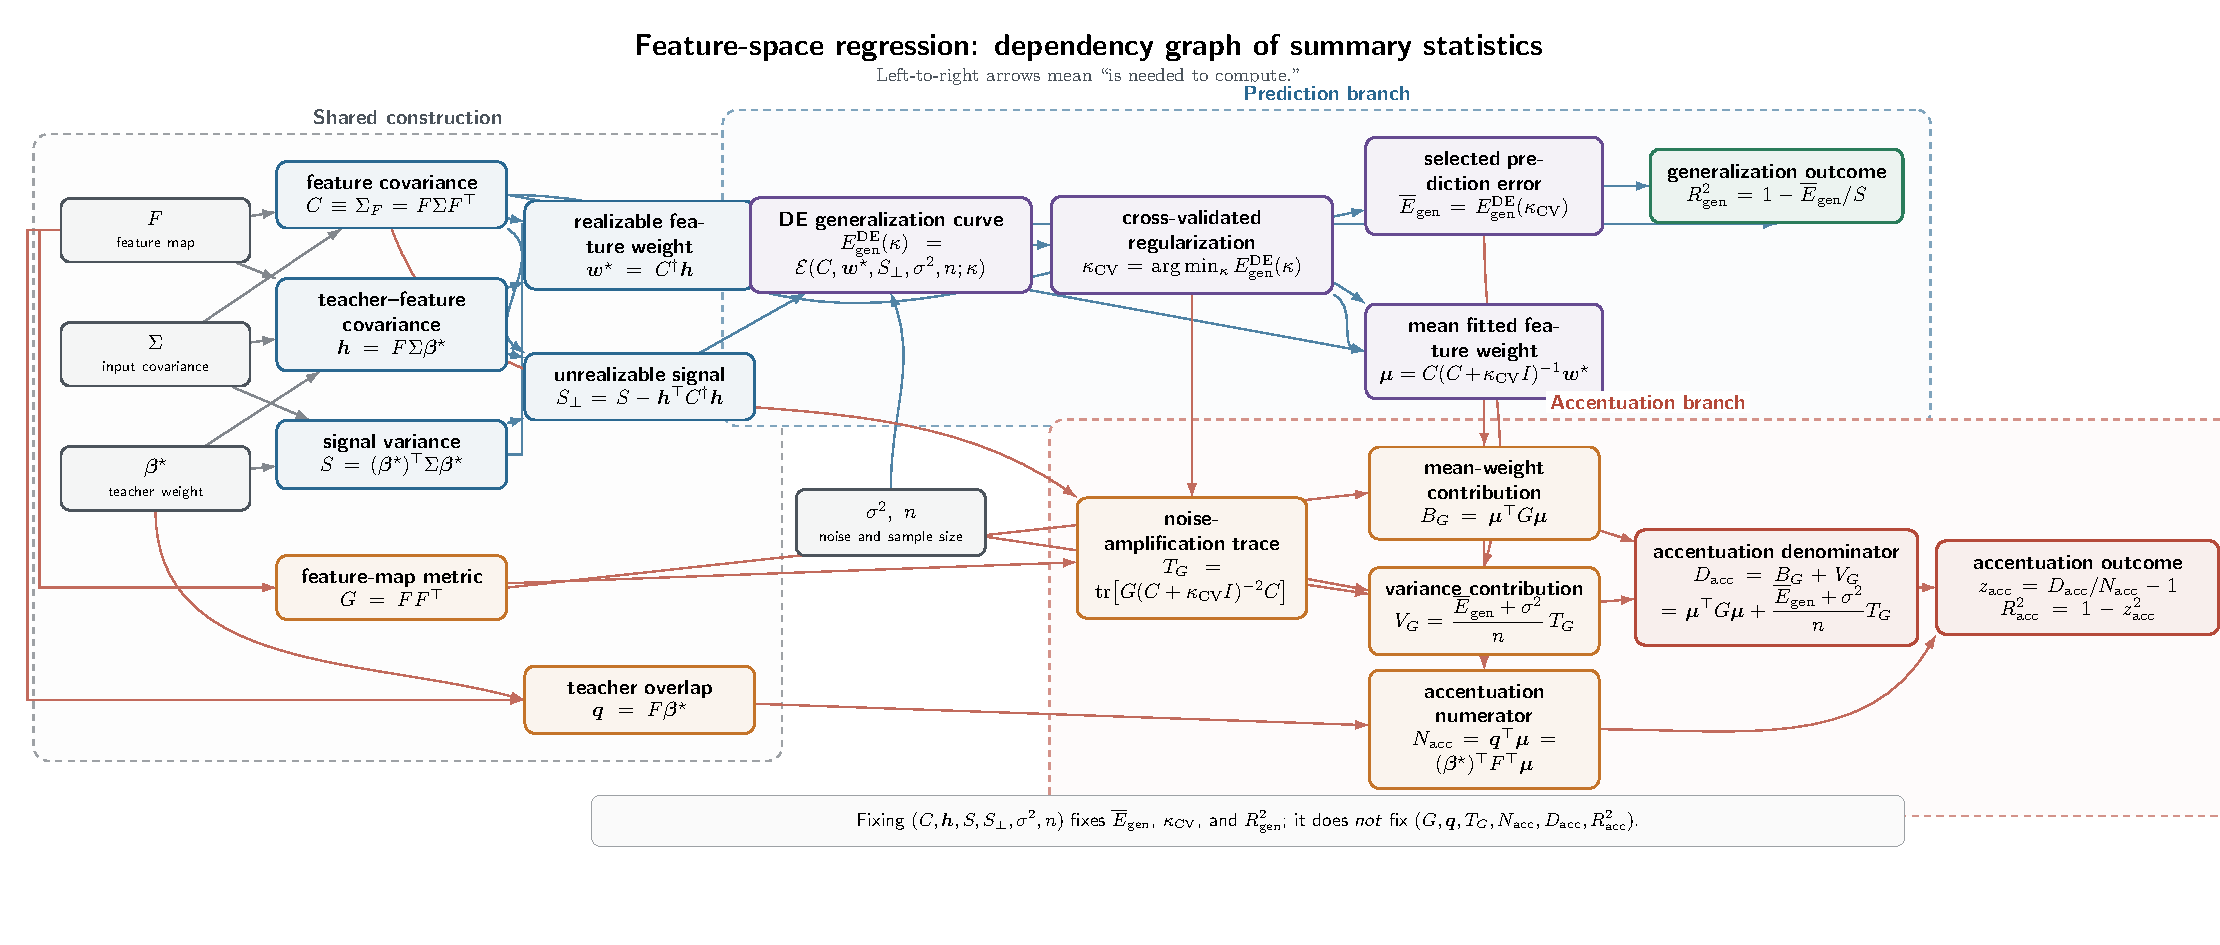
\includegraphics[width=1\textwidth]{figures/feature_summary_statistics_flow}
\caption{Dependency graph of the summary statistics of feature-space
regression.  Fixing $(C,h,S,S_\perp,\sigma^2,n)$ fixes the prediction
branch; the accentuation branch additionally needs $G=FF^\top$ and
$q=F\bstar$.  (TikZ source: \texttt{figures/theory/feature\_summary\_statistics\_flow.tex}
in the validation repository.)}
\label{fig:summary_stats_dep_graph}
\end{figure}

\subsection{The prediction-preserving gauge family}

Since prediction depends on $F$ only through $(C,h)$, any transformation of
$F$ that fixes these two objects leaves prediction, and hence its
cross-validated optimum, unchanged.  We characterize such transformations and
show that they generically change control.

\begin{prop}[Restatement of Proposition~\ref{prop:mr-gauge}]
\label{prop:app-feature-gauge}
Assume $\Sigma\succ0$.  For $Q\in O(d)$ with $Q\Sigma^{1/2}\bstar=\Sigma^{1/2}\bstar$,
the map $F_Q:=F\Sigma^{1/2}Q\Sigma^{-1/2}$ satisfies $F_Q\Sigma F_Q^\top=C$ and
$F_Q\Sigma\bstar=h$.  Consequently the joint Gaussian law of the training
pairs $(F_Q\x,y)$, the full curve $E_{gen,DE}(\kappa)$, and the DE-based
cross-validated penalty are the same for all $F_Q$ in the family, whereas
$G_Q=F_QF_Q^\top$ and $q_Q=F_Q\bstar$, and with them $\mu_N$, $\mu_D$ and all
accentuation metrics, vary in general.  If in addition
$Q\Sigma^{-1/2}\bstar=\Sigma^{-1/2}\bstar$, then $q_Q=q$ and only $G_Q$ varies.
For $\Sigma=I$ the family acts trivially on both prediction and control.
\end{prop}
\begin{proof}
Direct computation: $F_Q\Sigma F_Q^\top=F\Sigma^{1/2}QQ^\top\Sigma^{1/2}F^\top=C$
and $F_Q\Sigma\bstar=F\Sigma^{1/2}Q\Sigma^{1/2}\bstar=F\Sigma^{1/2}\Sigma^{1/2}\bstar=h$.
The pairs $(F_Q\x,y)$ are jointly Gaussian with covariance blocks
$\Cov(F_Q\x)=C$, $\Cov(F_Q\x,y)=h$, $\Var(y)=S+\sigma^2$, all invariant; hence
every functional of the training data, including the fitted $\hat w$, any
$K$-fold or leave-one-out cross-validation score, and the population risk
$E_{gen}=(\hat w-w^\star)^\top C(\hat w-w^\star)+S_\perp$, has the same law
across the family.  (Two members need not give the same CV choice on the
same realization of $X$, only the same distribution of choices.)  On the
other hand $G_Q=F\Sigma^{1/2}Q\Sigma^{-1}Q^\top\Sigma^{1/2}F^\top$ and
$q_Q=F\Sigma^{1/2}Q\Sigma^{-1/2}\bstar$ are not invariant unless $Q$ commutes
with $\Sigma$ on the relevant subspace, respectively fixes
$\Sigma^{-1/2}\bstar$.  For $\Sigma=I$, $F_Q=FQ$ with $Q\bstar=\bstar$, so
$G_Q=G$ and $q_Q=q$.
\end{proof}

\subsection{Constructing the family}

\paragraph{Whitened coordinates.}
The constraints are transparent in whitened coordinates.  Let
$A:=F\Sigma^{1/2}$, $b:=\Sigma^{1/2}\bstar$ and $c:=\Sigma^{-1/2}\bstar$, so
that $C=AA^\top$, $h=Ab$, $q=Ac$ and $G=A\Sigma^{-1}A^\top$.  Two maps
$F,F'$ are prediction-equivalent iff $A'b=Ab$ and $A'A'^\top=AA^\top$; the
first says that the rows of $A-A'$ are orthogonal to the whitened teacher
$b$.  A left rotation $F\mapsto O_pF$, $O_p\in O(p)$, is a change of feature
coordinates that is undone by $w\mapsto O_pw$ and produces no new control
behavior; the nontrivial freedom is on the right.

\paragraph{Right rotations with a fixed point.}
Let $W\in\R^{d\times(d-1)}$ be an orthonormal basis of $b^\perp$ and
$R\in O(d-1)$.  Then
\begin{equation}
O:=\frac{bb^\top}{\|b\|^2}+WRW^\top\in O(d),\qquad Ob=b,
\end{equation}
and $A_O:=AO$, $F_O:=A_O\Sigma^{-1/2}=F\Sigma^{1/2}O\Sigma^{-1/2}$ is the family
of Proposition~\ref{prop:app-feature-gauge}: a rotation of the whitened
feature map within the subspace orthogonal to the whitened teacher.  To
fix $q$ as well, take $W$ to span the complement of $\operatorname{span}(b,c)$.

\begin{example}[Two-dimensional rotation]
Let $\mathbf v_1,\mathbf v_2\perp b$ be orthonormal and let $\tilde A$ have
rows orthogonal to both.  Then
$A(\theta):=\tilde A+u(\theta)e_1\mathbf v_1^\top+v(\theta)e_1\mathbf v_2^\top$
has $A(\theta)A(\theta)^\top=\tilde A\tilde A^\top+(u^2+v^2)e_1e_1^\top$ and
$A(\theta)b=\tilde Ab$; any $u^2(\theta)+v^2(\theta)=\mathrm{const}$, e.g.
$(\cos\theta,\sin\theta)$, gives a one-parameter prediction-equivalent family
$F(\theta)=A(\theta)\Sigma^{-1/2}$.
\end{example}

\begin{example}[Resampling the null part]
Write $A=\frac{hb^\top}{\|b\|^2}+K\,Q_0$ with $K\in\R^{p\times r}$ and
$Q_0\in\R^{r\times d}$ having orthonormal rows orthogonal to $b$ (the SVD of
$A-hb^\top/\|b\|^2$).  Replacing $Q_0$ by any $Q_\phi$ with orthonormal rows
orthogonal to $b$ leaves $A_\phi b=h$ and
$A_\phi A_\phi^\top=hh^\top/\|b\|^2+KK^\top$ unchanged.  This gives a
constructive recipe: (i) from $(\Sigma,F,\bstar)$ form $A$, $b$, $h$;
(ii) take the SVD of the residual $A-hb^\top/\|b\|^2$; (iii) replace its
right singular vectors by a random orthonormal frame in $b^\perp$.  Random
draws from this recipe generate the ``population'' of equally predictive
feature maps used in the experiments.
\end{example}

\begin{proof}[Proof of Corollary~\ref{cor:mr-rotation}]
Let $P$ carry the components of $A$ that fix $Ab$ (and optionally $Ac$), and
let $R,V$ be row frames with $PR^\top=PV^\top=0$, $RV^\top=0$, $RR^\top=VV^\top$,
and $Rb=Vb=0$.  For $A(t)=P+\sqrt{1-t}\,R+\sqrt t\,V$ all cross terms vanish
and
\[
A(t)A(t)^\top=PP^\top+(1-t)RR^\top+tVV^\top=PP^\top+RR^\top,\qquad A(t)b=Pb,
\]
so $F(t)=A(t)\Sigma^{-1/2}$ lies in the family for every $t\in[0,1]$.
Choosing $R$ supported on high-variance and $V$ on low-variance eigendirections
of $\Sigma$ makes $G(t)=A(t)\Sigma^{-1}A(t)^\top$ acquire the factor
$s_k^{-1}$ of the tail directions as $t\to1$, so $\operatorname{Tr}G(t)$ and
$T_F$ grow without bound while every prediction summary is constant.
\end{proof}

\begin{example}[Aligned features, discrete version]
In the eigenbasis of $\Sigma=\operatorname{diag}(\lambda_1,\lambda_H,\lambda_L)$
with $\bstar=(1,0,0)^\top$, the two maps
\[
F_1=\begin{pmatrix}1&0&0\\0&\lambda_H^{-1/2}&0\end{pmatrix},\qquad
F_2=\begin{pmatrix}1&0&0\\0&0&\lambda_L^{-1/2}\end{pmatrix}
\]
have the same $C=\operatorname{diag}(\lambda_1,1)$ and the same $h$, hence the
same generalization error and cross-validated penalty, but
$G_1=\operatorname{diag}(1,\lambda_H^{-1})$ versus
$G_2=\operatorname{diag}(1,\lambda_L^{-1})$: the second feature of $F_2$ reads
a low-variance direction and back-propagates estimation noise into it with
gain $\lambda_L^{-1}\gg\lambda_H^{-1}$.
\end{example}

\begin{figure}[t]
\centering
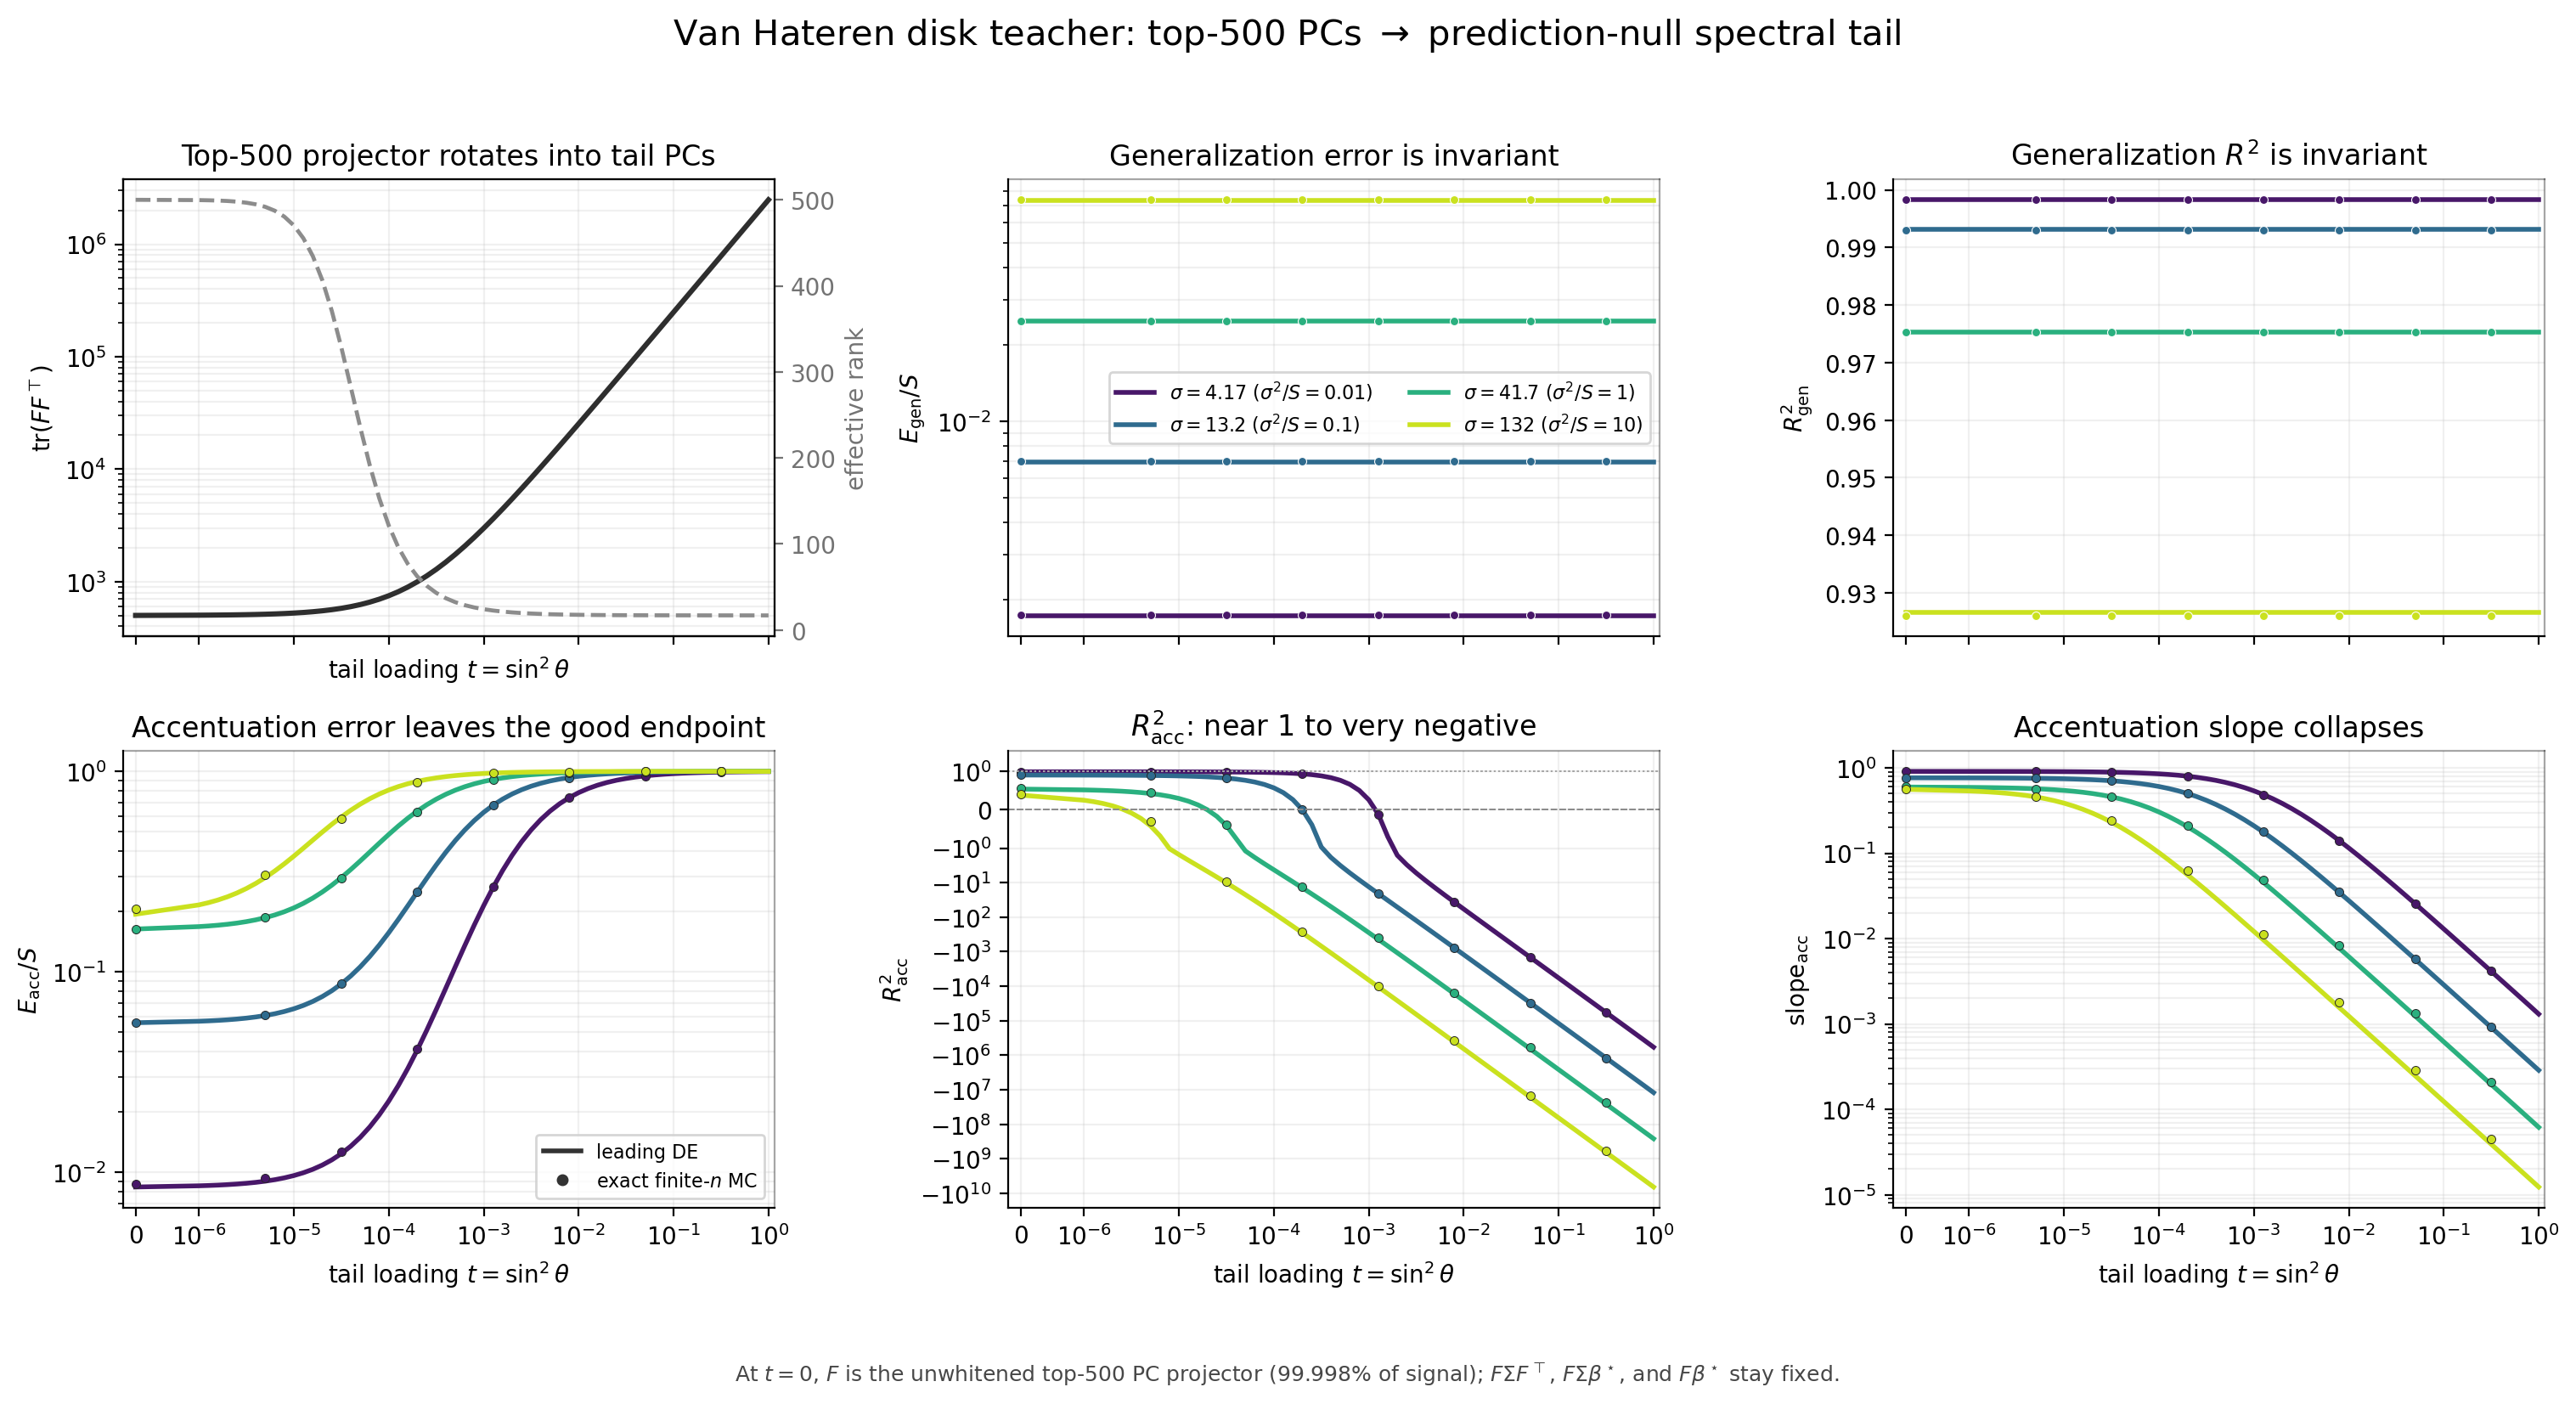
\includegraphics[width=1\linewidth]{figures/VanHateren_Top500PC_prediction_null_feature_rotation}\\
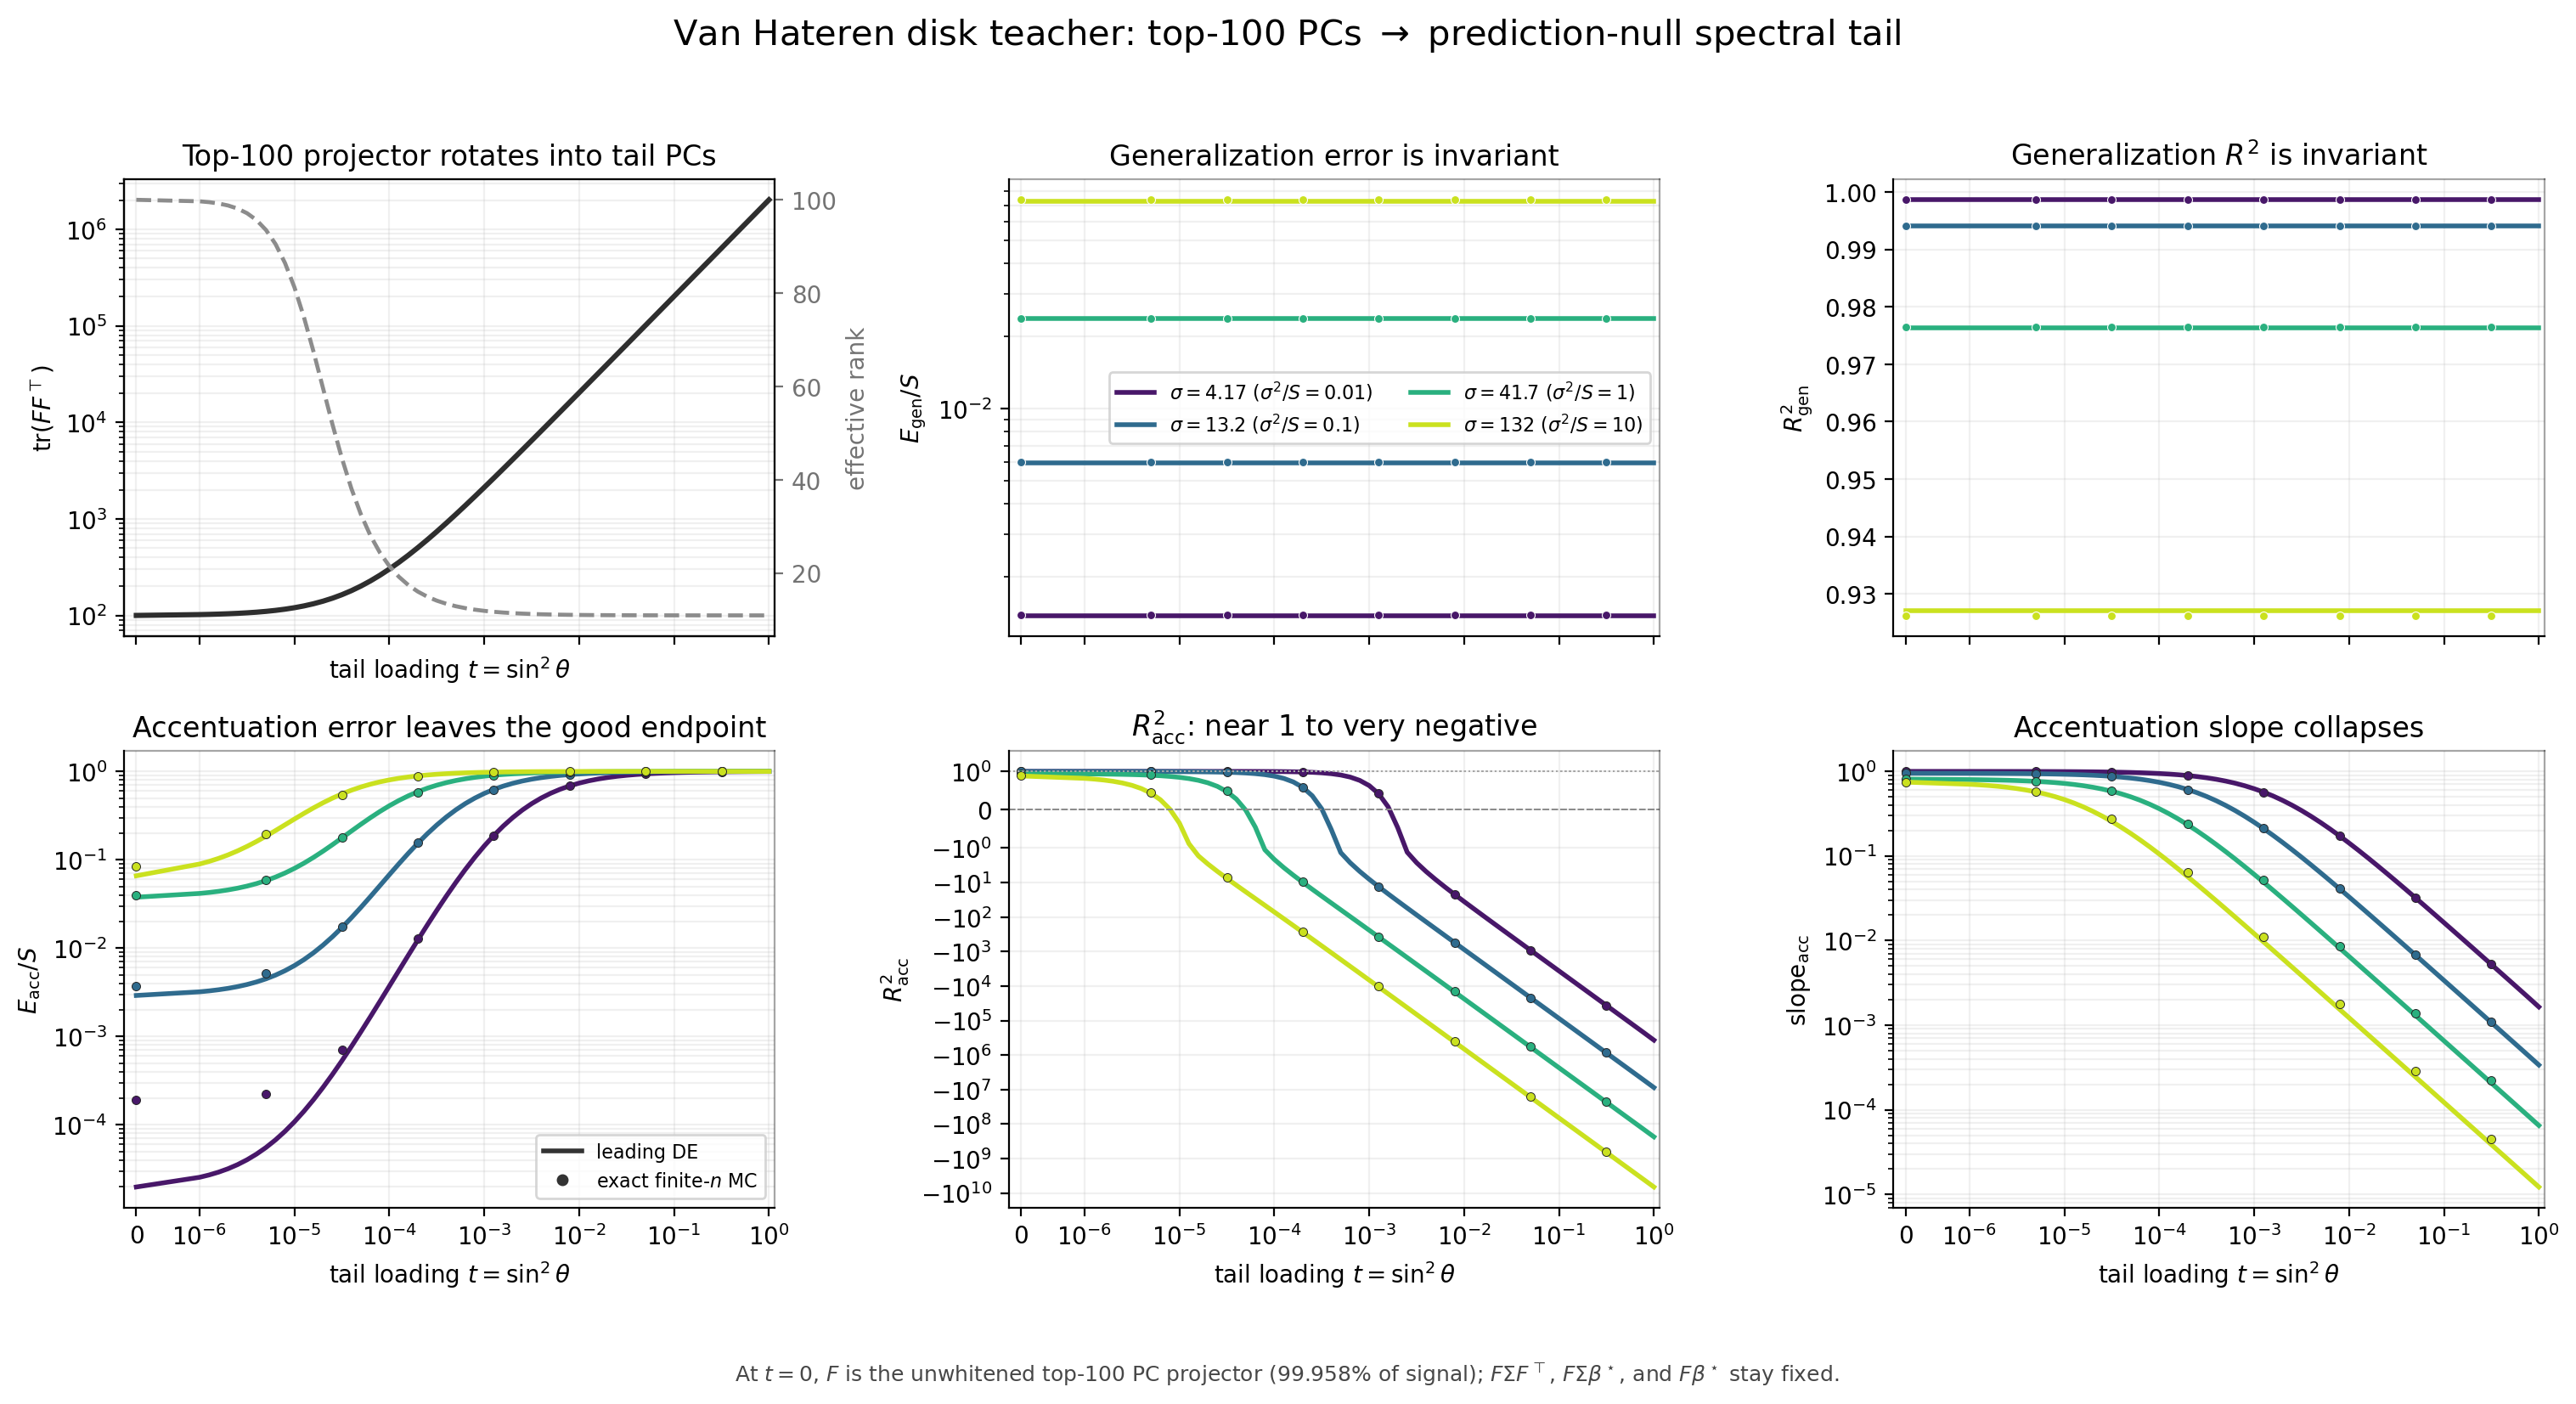
\includegraphics[width=1\linewidth]{figures/VanHateren_Top100PC_prediction_null_feature_rotation}
\caption{\textbf{Continuous prediction-null rotation on van Hateren images}
(Corollary~\ref{cor:mr-rotation}), starting from the top-500 (top) and
top-100 (bottom) PC projectors and rotating their null part into the
spectral tail.  Generalization error, $R^2_{gen}$ and the selected penalty are
exactly constant in the tail loading $t$, while $\operatorname{Tr}(FF^\top)$,
accentuation error, $R^2_{acc}$ and slope change by orders of magnitude.
Lines: leading DE; markers: finite-$n$ Monte Carlo.}
\label{fig:app-null-rotation}
\end{figure}

\subsection{A spectral diagnostic for fragile feature maps}
\label{sec:app-feature-fragility}

The variance contribution to the accentuation denominator carries the
response-independent factor
\begin{equation}
T_F(\kappa):=\operatorname{Tr}\big[FF^\top(\Sigma_F+\kappa I)^{-2}\Sigma_F\big],
\label{eq:feature-fragility-trace}
\end{equation}
which makes precise when estimation error that is modest in prediction
geometry becomes large after back-propagation to pixels.

\begin{prop}[Restatement of Proposition~\ref{prop:mr-fragility}]
\label{prop:feature-fragility-spectrum}
Let $\Sigma_F=\sum_ks_kv_kv_k^\top$ and $g_k:=F^\top v_k$ be the pixel
gradient of feature PC $k$.  Then
\begin{equation}
T_F(\kappa)=\sum_{k:s_k>0}\frac{s_k}{(s_k+\kappa)^2}\|g_k\|^2
=\sum_{k:s_k>0}\Big(\frac{s_k}{s_k+\kappa}\Big)^2\frac{\|g_k\|^2}{g_k^\top\Sigma g_k}.
\label{eq:feature-fragility-spectrum}
\end{equation}
\end{prop}
\begin{proof}
Cyclic invariance of the trace and the eigendecomposition of $\Sigma_F$ give
the first equality; $s_k=v_k^\top F\Sigma F^\top v_k=g_k^\top\Sigma g_k$
gives the second.
\end{proof}

\begin{remark}[Prediction-protected but control-fragile directions]
The ratio $\|g_k\|^2/g_k^\top\Sigma g_k$ compares the Euclidean energy of the
back-propagated PC gradient with its energy under the natural-image
covariance; it is large when $g_k$ concentrates on low-variance, typically
high-spatial-frequency, input directions.  The ridge factor
$(s_k/(s_k+\kappa))^2$ weights feature PCs that survive regularization.
Control is therefore fragile when even the well-resolved feature PCs
back-propagate into low-variance input directions.  $T_F$ can vary while
every prediction summary and $E_{gen,DE}$ remain fixed, and it can be
computed from the map and the image statistics alone.  In the nonlinear
diagnostic of Section~\ref{sec:app-nonlinear-diagnostic} the per-PC gradient
energies $\|g_k\|^2$ are replaced by local Jacobian energies.
\end{remark}

\section{Corrections for ratios of random quadratic forms}
\label{sec:app-ratio-approximations}
\label{sec:app-ratio-corrections}

\begingroup\color{red}
\begin{proposition}[Second-order expansion for the random ratio]
\label{prop:app-ratio-delta}
Let $N=\mu_N+\delta_N$ and $D=\mu_D+\delta_D$, with nonzero means and
fluctuations small enough for a second-order Taylor expansion. Then
\begin{align}
\mathbb E\!\left[\frac ND\right]
&\approx\frac{\mu_N}{\mu_D}
\left(1-\frac{\operatorname{Cov}(N,D)}{\mu_N\mu_D}
+\frac{\operatorname{Var}(D)}{\mu_D^2}\right),\\
\mathbb E\!\left[\left(\frac ND\right)^2\right]
&\approx\frac{\mu_N^2}{\mu_D^2}
\left(1+\frac{\operatorname{Var}(N)}{\mu_N^2}
-4\frac{\operatorname{Cov}(N,D)}{\mu_N\mu_D}
+3\frac{\operatorname{Var}(D)}{\mu_D^2}\right).
\end{align}
The ratio-of-DE approximation retains only the leading mean ratio.  The
second-order terms become consequential when the leading calibration bias is
small or the denominator has appreciable relative variance.
\end{proposition}
\endgroup

\subsection{Approximating the expectation of a ratio}

RMT gives cleaner control of $N$ and $D$ separately than of their ratio.
The leading approximation replaces the expectation of a ratio by the ratio
of deterministic equivalents. To quantify the resulting error, write
$\mathbb{E}[N]=\mu_N$, $\mathbb{E}[D]=\mu_D$ and expand around the two means:
\begin{align*}
\frac{N}{D} & =\frac{\mu_{N}+\delta_{N}}{\mu_{D}+\delta_{D}}\\
 & =\frac{\mu_{N}+\delta_{N}}{\mu_{D}+\delta_{D}}-\frac{\mu_{N}}{\mu_{D}}+\frac{\mu_{N}}{\mu_{D}}\\
 & =\frac{\mu_{N}}{\mu_{D}}+\frac{\delta_{N}\mu_{D}-\delta_{D}\mu_{N}}{\mu_{D}\mu_{D}(\frac{\mu_{D}+\delta_{D}}{\mu_{D}})}\\
 & =\frac{\mu_{N}}{\mu_{D}}+\frac{\delta_{N}\mu_{D}-\delta_{D}\mu_{N}}{\mu_{D}^{2}}(1+\frac{\delta_{D}}{\mu_{D}})^{-1}\\
 & =\frac{\mu_{N}}{\mu_{D}}+\frac{\delta_{N}\mu_{D}-\delta_{D}\mu_{N}}{\mu_{D}^{2}}(1-\frac{\delta_{D}}{\mu_{D}}+\frac{\delta_{D}^{2}}{\mu_{D}^{2}}+...)
\end{align*}

Note the first non-trivial order is the 2nd order in $\delta$, which
gives
\begin{align*}
\frac{N}{D} & =\frac{\mu_{N}}{\mu_{D}}+\frac{\delta_{N}\mu_{D}-\delta_{D}\mu_{N}}{\mu_{D}^{2}}-\frac{\delta_{D}}{\mu_{D}}\frac{\delta_{N}\mu_{D}-\delta_{D}\mu_{N}}{\mu_{D}^{2}}+o((\frac{\delta}{\mu})^{3})\\
 & =\frac{\mu_{N}}{\mu_{D}}+\frac{\delta_{N}}{\mu_{D}}-\frac{\delta_{D}\mu_{N}}{\mu_{D}^{2}}-\frac{\delta_{D}\delta_{N}}{\mu_{D}^{2}}+\frac{\delta_{D}^{2}\mu_{N}}{\mu_{D}^{3}}+o((\frac{\delta}{\mu})^{3})
\end{align*}

When taking expectation the first two orders gives
\[
\mathbb{E}\big[\frac{N}{D}\big]\approx\frac{\mu_{N}}{\mu_{D}}-\frac{\mathrm{Cov}(D,N)}{\mu_{D}^{2}}+\frac{\mathrm{Var}(D)\mu_{N}}{\mu_{D}^{3}}+\mathbb{E}\big[o((\frac{\delta}{\mu})^{3})\big]
\]

Similarly let's consider the other useful terms, i.e. the squared
ratio, and their expansion.
\begin{align*}
(\frac{N}{D})^{2} & =\frac{(\mu_{N}+\delta_{N})^{2}}{(\mu_{D}+\delta_{D})^{2}}\\
 & =\frac{\mu_{N}^{2}+2\mu_{N}\delta_{N}+\delta_{N}^{2}}{\mu_{D}^{2}+2\mu_{D}\delta_{D}+\delta_{D}^{2}}\\
 & =\frac{\mu_{N}^{2}+2\mu_{N}\delta_{N}+\delta_{N}^{2}}{\mu_{D}^{2}}(\frac{\mu_{D}^{2}+2\mu_{D}\delta_{D}+\delta_{D}^{2}}{\mu_{D}^{2}})^{-1}\\
 & =\frac{\mu_{N}^{2}+2\mu_{N}\delta_{N}+\delta_{N}^{2}}{\mu_{D}^{2}}(1-(2\frac{\delta_{D}}{\mu_{D}}+\frac{\delta_{D}^{2}}{\mu_{D}^{2}})+(2\frac{\delta_{D}}{\mu_{D}}+\frac{\delta_{D}^{2}}{\mu_{D}^{2}})^{2}+o((2\frac{\delta_{D}}{\mu_{D}}+\frac{\delta_{D}^{2}}{\mu_{D}^{2}})^{3}))\\
 & =\frac{\mu_{N}^{2}+2\mu_{N}\delta_{N}+\delta_{N}^{2}}{\mu_{D}^{2}}(1-2\frac{\delta_{D}}{\mu_{D}}+3\frac{\delta_{D}^{2}}{\mu_{D}^{2}}+o((\frac{\delta_{D}}{\mu_{D}})^{3}))\\
 & =\frac{\mu_{N}^{2}}{\mu_{D}^{2}}(1-2\frac{\delta_{D}}{\mu_{D}}+3\frac{\delta_{D}^{2}}{\mu_{D}^{2}}+o((\frac{\delta_{D}}{\mu_{D}})^{3}))+\frac{2\mu_{N}\delta_{N}}{\mu_{D}^{2}}(1-2\frac{\delta_{D}}{\mu_{D}}+o((\frac{\delta_{D}}{\mu_{D}})^{2}))+\frac{\delta_{N}^{2}}{\mu_{D}^{2}}(1+o((\frac{\delta_{D}}{\mu_{D}})))\\
 & =\frac{\mu_{N}^{2}}{\mu_{D}^{2}}-2\frac{\mu_{N}^{2}}{\mu_{D}^{2}}\frac{\delta_{D}}{\mu_{D}}+3\frac{\mu_{N}^{2}}{\mu_{D}^{2}}\frac{\delta_{D}^{2}}{\mu_{D}^{2}}+\frac{2\mu_{N}\delta_{N}}{\mu_{D}^{2}}-4\frac{\mu_{N}\delta_{N}}{\mu_{D}^{2}}\frac{\delta_{D}}{\mu_{D}}+\frac{\delta_{N}^{2}}{\mu_{D}^{2}}+o((\frac{\delta}{\mu})^{3})
\end{align*}

\begin{align*}
\mathbb{E}[(\frac{N}{D})^{2}] & \approx\frac{\mu_{N}^{2}}{\mu_{D}^{2}}+3\frac{\mu_{N}^{2}}{\mu_{D}^{2}}\frac{\mathbb{E}[\delta_{D}^{2}]}{\mu_{D}^{2}}-4\frac{\mu_{N}}{\mu_{D}^{2}}\frac{\mathbb{E}[\delta_{N}\delta_{D}]}{\mu_{D}}+\frac{\mathbb{E}[\delta_{N}^{2}]}{\mu_{D}^{2}}+o((\frac{\delta}{\mu})^{3})\\
 & \approx\frac{\mu_{N}^{2}}{\mu_{D}^{2}}+3\frac{\mu_{N}^{2}}{\mu_{D}^{2}}\frac{\mathrm{Var}[D]}{\mu_{D}^{2}}-4\frac{\mu_{N}}{\mu_{D}}\frac{\mathrm{Cov}[N,D]}{\mu_{D}^{2}}+\frac{\mathrm{Var}[N]}{\mu_{D}^{2}}+o((\frac{\delta}{\mu})^{3})
\end{align*}

\noindent\fbox{\begin{minipage}[t]{1\columnwidth - 2\fboxsep - 2\fboxrule}%
In summary the leading order correction to the fraction and power
are
\begin{align*}
\mathbb{E}\big[\frac{N}{D}\big] & \approx\frac{\mu_{N}}{\mu_{D}}-\frac{\mathrm{Cov}(D,N)}{\mu_{D}^{2}}+\frac{\mathrm{Var}(D)\mu_{N}}{\mu_{D}^{3}}\\
\mathbb{E}[(\frac{N}{D})^{2}] & \approx\frac{\mu_{N}^{2}}{\mu_{D}^{2}}+3\frac{\mu_{N}^{2}}{\mu_{D}^{2}}\frac{\mathrm{Var}[D]}{\mu_{D}^{2}}-4\frac{\mu_{N}}{\mu_{D}}\frac{\mathrm{Cov}[N,D]}{\mu_{D}^{2}}+\frac{\mathrm{Var}[N]}{\mu_{D}^{2}}
\end{align*}

It can be written in more normalized (dimensionless) forms
\begin{align*}
\mathbb{E}\big[\frac{N}{D}\big] & \approx\frac{\mu_{N}}{\mu_{D}}\Big(1-\frac{\mathrm{Cov}(D,N)}{\mu_{N}\mu_{D}}+\frac{\mathrm{Var}(D)}{\mu_{D}^{2}}\Big)\\
\mathbb{E}[(\frac{N}{D})^{2}] & \approx\frac{\mu_{N}^{2}}{\mu_{D}^{2}}\Big(1+3\frac{\mathrm{Var}[D]}{\mu_{D}^{2}}-4\frac{\mathrm{Cov}[N,D]}{\mu_{N}\mu_{D}}+\frac{\mathrm{Var}[N]}{\mu_{N}^{2}}\Big)
\end{align*}
%
\end{minipage}}

Thus, for the 0th order term we need to compute $\mu_{N}$,$\mu_{D}$;

For the 1st order correction, we need to compute $\mathrm{Var}[D]$,
$\mathrm{Cov}[N,D]$, $\mathrm{Var}[N]$ normalized by the corresponding
mean.



\subsection{Second-order delta expansion}
\label{sec:app-ratio-delta}

The leading correction follows by retaining second-order terms.
\begin{align*}
\mathbb{E}\big[\frac{N}{D}\big] & \approx\frac{\mu_{N}}{\mu_{D}}\Big(1-\frac{\mathrm{Cov}(D,N)}{\mu_{N}\mu_{D}}+\frac{\mathrm{Var}(D)}{\mu_{D}^{2}}\Big)\\
\mathbb{E}[(\frac{N}{D})^{2}] & \approx\frac{\mu_{N}^{2}}{\mu_{D}^{2}}\Big(1+3\frac{\mathrm{Var}[D]}{\mu_{D}^{2}}-4\frac{\mathrm{Cov}[N,D]}{\mu_{N}\mu_{D}}+\frac{\mathrm{Var}[N]}{\mu_{N}^{2}}\Big)
\end{align*}


\subsection{Gaussian distributional approximation: ``Gaussian distributional
DE'' }
\label{sec:app-ratio-gaussian}

Another way to estimate this ratio is to say $\bhat$ is a Gaussian
random variable, then express its expectation and covariance -- note
that the expectation and covariance both concentrates via DE, we can
denote as $m_{DE},V_{DE}$, then they won't depend on $X$ realization
explicitly.

So we can sample $\bhat$ from this surrogate Gaussian distribution
then evaluate
\[
\mathbb{E}_{\bhat\sim\mathcal{N}(m_{DE},V_{DE})}\big[\frac{{\bhat}^{\top}\bstar}{{\bhat}^{\top}\bhat}\big]
\]

with bootstrap averaging.

\subsection{Theory of peer review error}

We next characterize what peer-review error measures. Recall the
evaluation metrics of peer review, where the generating model has
weight $\bprime$, and the predicting model has weight $\bhat$
\begin{align*}
\mathrm{MSE}_{\text{peer rev}}= & \mathrm{Var}[\alpha^{\prime}]\big({\bprime}^{\top}(\bhat-\bstar)\big)^{2}\\
R_{\text{peer rev}}^{2}= & 1-\big(\frac{{\bprime}^{\top}\bhat}{{\bprime}^{\top}\bstar}-1\big)^{2}\\
\mathrm{slope}_{\text{peer rev}}= & \frac{{\bprime}^{\top}\bstar}{{\bprime}^{\top}\bhat}
\end{align*}

\begin{table}
\begin{centering}
\begin{tabular}{|c|c|c|c|}
\hline
 & Peer Review & Peer Review on Perfect Accentuator & Accentuation\tabularnewline
\hline
\hline
MSE & $\mathrm{Var}[\alpha]\big({\bprime}^{\top}(\bhat-\bstar)\big)^{2}$ & $\mathrm{Var}[\alpha]\big({\bstar}^{\top}(\bhat-\bstar)\big)^{2}$ & $\mathrm{Var}[\alpha]\big({\bhat}^{\top}(\bhat-\bstar)\big)^{2}$\tabularnewline
\hline
R2 & $1-\big(\frac{{\bprime}^{\top}\bhat}{{\bprime}^{\top}\bstar}-1\big)^{2}$ & $1-\big(\frac{{\bstar}^{\top}\bhat}{{\bstar}^{\top}\bstar}-1\big)^{2}$ & $1-\big(\frac{{\bhat}^{\top}\bhat}{{\bhat}^{\top}\bstar}-1\big)^{2}$\tabularnewline
\hline
slope & $\frac{{\bprime}^{\top}\bstar}{{\bprime}^{\top}\bhat}$ & $\frac{{\bstar}^{\top}\bstar}{{\bstar}^{\top}\bhat}$ & $\frac{{\bhat}^{\top}\bstar}{{\bhat}^{\top}\bhat}$\tabularnewline
\hline
\end{tabular}
\par\end{centering}
\caption{Comparison of evaluation metrics when evaluating on perfect evaluating
model $\bprime=\bstar$.}
\end{table}


\paragraph{Perfect peer direction.}

Consider the idealized case in which the generating model is aligned with the
ground truth, $\bprime=\bstar$.

The generation--evaluation asymmetry is then explicit in the two slope ratios:
\begin{align*}
\mathrm{slope}_{acc}= & \frac{{\bhat}^{\top}\bstar}{{\bhat}^{\top}\bhat} & \mathrm{slope}_{\text{peer rev}}= & \frac{{\bstar}^{\top}\bstar}{{\bstar}^{\top}\bhat}
\end{align*}

Conditionally on a realized $\bhat$, the peer-review slope is
$\|\bstar\|^2/({\bstar}^\top\bhat)$. Its expectation is again an expectation
of a random ratio and must be handled by the approximations developed above;
it is not generally the ratio obtained by replacing the denominator with its
mean.




\section{Nonlinear gradient diagnostic}
\label{sec:app-nonlinear-diagnostic}
\label{sec:app-nonlinear-feature-diagnostic}

The linear-feature DE does not directly become a theorem for a nonlinear
map $\phi:\mathbb R^d\to\mathbb R^p$.  It nevertheless suggests a local
diagnostic.  Let
\begin{equation}
  J_\phi(x):=\frac{\partial\phi(x)}{\partial x}\in\mathbb R^{p\times d},
  \qquad
  \Sigma_\phi:=\operatorname{Cov}_{x\sim P_x}[\phi(x)]
  =\sum_k s_kv_kv_k^\top.
\end{equation}
Replacing the constant linear Jacobian $F$ by $J_\phi(x)$ motivates
\begin{equation}
  T_\phi(x,\kappa)
  :=\sum_k\frac{s_k}{(s_k+\kappa)^2}
       \|J_\phi(x)^\top v_k\|^2.
  \label{eq:nonlinear-local-fragility}
\end{equation}
Here $J_\phi(x)^\top v_k=\nabla_x[v_k^\top\phi(x)]$ is the input gradient
of feature PC $k$.  Unlike the linear case, generally
$s_k\neq\nabla_x[v_k^\top\phi(x)]^\top\Sigma
\nabla_x[v_k^\top\phi(x)]$; therefore Eq.~\eqref{eq:nonlinear-local-fragility}
is a diagnostic motivated by the linear theory, not a deterministic
equivalent for nonlinear regression.

\paragraph{Finite-neighborhood versions.}
An exact Jacobian at the seed may be too local for a long accentuation path.
For $z\sim\mathcal N(0,I_d)$ and neighborhood scale $\tau$, useful
PC-wise quantities include
\begin{align}
M_{smooth,k}
  &:=\left\|\mathbb E_z[J_\phi(x_0+\tau z)^\top v_k]\right\|^2,\\
M_{neighbor,k}
  &:=\mathbb E_z\left[\|J_\phi(x_0+\tau z)^\top v_k\|^2\right],\\
M_{var,k}
  &:=\tau^{-2}\operatorname{Var}_z[v_k^\top\phi(x_0+\tau z)],\\
M_{step,k}
  &:=\tau^{-2}\mathbb E_z\left[
       (v_k^\top\phi(x_0+\tau z)-v_k^\top\phi(x_0))^2\right].
\label{eq:nonlinear-neighborhood-estimators}
\end{align}
These estimators agree only in the locally linear, small-$\tau$ limit and
otherwise answer different questions: squared mean gradient, mean squared
gradient, response variance, and finite-step sensitivity, respectively.

\paragraph{Stein estimator.}
For differentiable $\phi$ with suitable integrability, Stein's identity gives
\begin{equation}
\mathbb E_z[J_\phi(x_0+\tau z)^\top v_k]
=\frac{1}{\tau}\mathbb E_z[(v_k^\top\phi(x_0+\tau z))z].
\label{eq:nonlinear-stein-estimator}
\end{equation}
Centering by $\phi(x_0)$ is a control variate, and antithetic pairs
$x_0\pm\tau z$ replace the numerator by
$v_k^\top[\phi(x_0+\tau z)-\phi(x_0-\tau z)]/2$.  These changes preserve
the population identity while reducing Monte Carlo variance.  Empirical
validation should report the neighborhood scale, number of probes, and
estimator variance rather than treating a noisy Jacobian estimate as exact.

\subsection{Empirical validation against neuronal control}
\label{sec:app-nonlinear-biological-validation}
We evaluated the diagnostic on 25 neuronal sites crossed with ten encoding
models. Each feature geometry used the fitted RidgeCV penalty and held-out
natural-image error in the same response units. A single cross-session affine
calibration was fitted per site on natural-image anchors and then shared
across all models. To isolate model ordering from site-level difficulty, both
the log diagnostic and biological endpoint were centered within site.

Among the nine trained models ($225$ site--model pairs), exact-local
$V_\phi$ achieved direction-aligned Pearson correlations $r=0.616$ with
control slope and $r=0.442$ with direct control MSE. The corresponding
held-out generalization-MSE correlations were $0.034$ and $-0.069$.
Neighborhood smoothing retained strong ordering and, for slope, reached
$r=0.605$ at noise scale $16/255$. Restricting to seven conventionally
trained models attenuated the exact-local slope association to $r=0.189$;
thus part of the full ordering is carried by the robust-model contrast.
These values are descriptive repeated-measures associations, not an estimate
of absolute control response and not an independent-observation significance
test. Figure~\ref{fig:nonlinear-biological-validation} reports the complete
paper-facing comparison.
\endgroup




\section{Random-matrix toolkit}
\label{sec:app-rmt-toolkit}
\label{sec:app-de-toolkit}

\subsection{Deterministic equivalence relationships}
\label{sec:app-de-identities}

Denote $1/\varphi(-z)=\kappa(z)$

Then we have the equivalence and flip the sign of $z$
\[
\mbox{tr}\bigl[A\,(\widehat{\Sigma}+zI)^{-1}\bigr]\sim\frac{\kappa(z)}{z}\mbox{tr}\bigl[A\bigl(\Sigma+\kappa(z)I\bigr)^{-1}\bigr]
\]
\begin{align*}
\mbox{tr}\bigl[A(\widehat{\Sigma}+zI)^{-1}B(\widehat{\Sigma}+zI)^{-1}\bigr] & \sim\frac{\kappa(z)^{2}}{z^{2}\,}\mbox{tr}\bigl[A\,\bigl(\Sigma+\kappa(z)I\bigr)^{-1}\,B\,\bigl(\Sigma+\kappa(z)I\bigr)^{-1}\bigr]\\
 & \quad+\frac{\kappa(z)^{2}}{z^{2}}\frac{1}{n-\mathrm{df}_{2}\bigl(\kappa(z)\bigr)}\mbox{tr}\bigl[A\,\bigl(\Sigma+\kappa(z)I\bigr)^{-2}\Sigma\bigr]\mbox{tr}\bigl[B\,\bigl(\Sigma+\kappa(z)I\bigr)^{-2}\Sigma\bigr]
\end{align*}

Using equivalent form
\[
\mbox{tr}\bigl[A\widehat{\Sigma}(\widehat{\Sigma}+zI)^{-1}\bigr]\sim\mbox{tr}\bigl[A\,\Sigma\,\bigl(\Sigma+\kappa(z)I\bigr)^{-1}\bigr]
\]
\begin{align*}
\mbox{tr}\bigl[A\,\widehat{\Sigma}\,(\widehat{\Sigma}+zI)^{-1}\,B\,\widehat{\Sigma}\,(\widehat{\Sigma}+zI)^{-1}\bigr] & \sim\mbox{tr}\bigl[A\,\Sigma\,\bigl(\Sigma+\kappa(z)I\bigr)^{-1}\,B\,\Sigma\,\bigl(\Sigma+\kappa(z)I\bigr)^{-1}\bigr]\\
 & \quad+\frac{\kappa^{2}(z)}{n-\mathrm{df}_{2}\bigl(\kappa(z)\bigr)}\mbox{tr}\bigl[A\,\bigl(\Sigma+\kappa(z)I\bigr)^{-2}\Sigma\bigr]\mbox{tr}\bigl[B\,\bigl(\Sigma+\kappa(z)I\bigr)^{-2}\Sigma\bigr]
\end{align*}

where $\kappa(z)$ can be solved from self consistent equation

The self consistent variable is defined via $\varphi(z):=\mbox{tr}[(XX^{\top}-nzI)^{-1}]$,
then the self consistent equation for $\kappa(z):=\frac{1}{\varphi(-z)}$
is, where $\mu(s)$ is the spectral measure of covariance $\Sigma$
\[
\frac{1}{\varphi(z)}+z=\gamma\int_{0}^{\infty}\frac{s\ d\mu(s)}{1+s\varphi(z)}
\]
\begin{align*}
\frac{1}{\varphi(-z)}-z & =\gamma\int_{0}^{\infty}\frac{s\ d\mu(s)}{1+s\varphi(-z)}\\
\kappa(z)-z & =\gamma\int_{0}^{\infty}\frac{s\ d\mu(s)}{1+s\frac{1}{\kappa(z)}}\\
\kappa(z)-z & =\gamma\int_{0}^{\infty}\frac{\kappa(z)\ sd\mu(s)}{\kappa(z)+s}\\
\kappa(z)-z & =\gamma\kappa(z)\int_{0}^{\infty}\frac{sd\mu(s)}{\kappa(z)+s}\\
z & =\kappa(z)\Big[1-\gamma\int_{0}^{\infty}\frac{\ sd\mu(s)}{\kappa(z)+s}\Big]
\end{align*}

in matrix form
\[
\kappa(\lambda)-\lambda=\gamma\kappa(\lambda)\!\mathrm{tr}[\Sigma(\Sigma+\kappa(\lambda))^{-1}]
\]


\paragraph{Useful quantities and identities}

\begin{align*}
\mathrm{df}_{1}(\lambda) & :=\mbox{Tr}[\Sigma(\Sigma+\lambda I)^{-1}]\\
\mathrm{df}_{2}(\lambda) & :=\mbox{Tr}[\Sigma^{2}(\Sigma+\lambda I)^{-2}]
\end{align*}

With identities
\begin{align*}
\mathrm{df}_{2}(\kappa)-\mathrm{df}_{1}(\kappa) & =\mbox{Tr}[\Sigma^{2}(\Sigma+\kappa I)^{-2}]-\mbox{Tr}[\Sigma(\Sigma+\kappa I)^{-1}]\\
 & =\mbox{Tr}[\big(\Sigma(\Sigma+\kappa I)^{-1}-I\big)\Sigma(\Sigma+\kappa I)^{-1}]\\
 & =\kappa\mbox{Tr}[\Sigma(\Sigma+\kappa I)^{-2}]
\end{align*}

We have relationship
\[
\min(n,p)>\mathrm{df}_{2}(\kappa)>\mathrm{df}_{1}(\kappa)
\]


\paragraph{Two point equivalence}

As an immediate outcome, set $A=\Sigma$, $B=\frac{1}{n}XX^{T}$ as
white Wishart, then $A*B=\hat{\Sigma}$. Thus,
\[
\hat{\Sigma}(\lambda+\hat{\Sigma})^{-1}M\hat{\Sigma}(\lambda^{\prime}+\hat{\Sigma})^{-1}\simeq T_{\Sigma}MT_{\Sigma}^{\prime}+\kappa\kappa'G_{\Sigma}\Sigma G_{\Sigma}^{\prime}\frac{\mbox{Tr}\left[G_{\Sigma}^{\prime}\Sigma G_{\Sigma}M\right]}{n-\mathrm{df}_{2}(\kappa,\kappa')}
\]

in trace form we can write
\[
\mbox{Tr}\Big[A\hat{\Sigma}(\lambda+\hat{\Sigma})^{-1}B\hat{\Sigma}(\lambda^{\prime}+\hat{\Sigma})^{-1}\Big]\simeq\mbox{Tr}\big[AT_{\Sigma}BT_{\Sigma}^{\prime}\big]+\frac{\kappa\kappa'}{n-\mathrm{df}_{2}(\kappa,\kappa')}\mbox{Tr}\big[AG_{\Sigma}\Sigma G_{\Sigma}^{\prime}\big]\mbox{Tr}\big[G_{\Sigma}^{\prime}\Sigma G_{\Sigma}B\big]
\]
where $T_{A}:=A(A+\kappa)^{-1},T_{A}^{\prime}:=A(A+\kappa^{\prime})^{-1}$,
$G_{A}:=(A+\kappa)^{-1},G_{A}^{\prime}:=(A+\kappa^{\prime})^{-1}$.
and $\mathrm{df}_{2}(\kappa,\kappa'):=\mathrm{tr}[A^{2}G_{A}G_{A}^{\prime}]$,
$q=N/P$ and $A\in\mathbb{R}^{N\times N}$.

\subsection{General algebraic quantity}

In the derivation, we will heavily rely on the two family of quantities
\begin{align*}
B_{p,q}(\kappa) & =\sum_{k=1}^{d}\frac{s_{k}^{p}}{(s_{k}+\kappa)^{q}}b_{k}^{2}\\
\mathrm{df}_{p,q}(\kappa) & =\sum_{k=1}^{d}\frac{s_{k}^{p}}{(s_{k}+\kappa)^{q}}
\end{align*}

where the classic short hand are special cases of these.
\begin{align*}
\mathrm{df}_{1}(\kappa) & \equiv\mathrm{df}_{1,1}(\kappa)\\
\mathrm{df}_{2}(\kappa) & \equiv\mathrm{df}_{2,2}(\kappa)
\end{align*}

The recursion starts from the meaningful quantities
\begin{align*}
\mathrm{df}_{0,0}(\kappa) & =d\\
B_{0,0}(\kappa) & =\|\bstar\|^{2}=\sum b_{k}^{2}
\end{align*}

They can be interpreted as following
\begin{itemize}
\item $\mathrm{df}_{p,q}(\kappa)$ is a weighted \textbf{count} of spectral
modes, where the weighting function is $\frac{s_{k}^{p}}{(s_{k}+\kappa)^{q}}$.
In classic cases $p=q$ and these weighting functions range from $(0,1)$
so it's exactly counting the modes from 0,1.
\end{itemize}

\subsubsection{Inequalities}

Since $\kappa>0$,
\[
\frac{s_{k}}{(s_{k}+\kappa)}<1
\]

thus in general
\begin{align*}
B_{p,q}(\kappa) & \geq B_{p+1,q+1}(\kappa)\\
\mathrm{df}_{p,q}(\kappa) & \geq\mathrm{df}_{p+1,q+1}(\kappa)
\end{align*}

The classic inequality of
\[
d\geq\mathrm{df}_{1}(\kappa)\geq\mathrm{df}_{2}(\kappa)
\]

can be seen as a special case of
\[
\mathrm{df}_{0,0}(\kappa)\geq\mathrm{df}_{1,1}(\kappa)\geq\mathrm{df}_{2,2}(\kappa)
\]

Here we have the more general case
\[
\mathrm{df}_{0,1}(\kappa)\geq\mathrm{df}_{1,2}(\kappa)\geq\mathrm{df}_{2,3}(\kappa)
\]


\subsubsection{Recursion and Differential Identities}

They admits following recursion identities,
\[
\mathrm{df}_{p,q}(\kappa)=\mathrm{df}_{p+1,q+1}(\kappa)+\kappa\mathrm{df}_{p,q+1}(\kappa)
\]

Equivalently
\begin{align*}
\mathrm{df}_{p+1,q+1}(\kappa)-\mathrm{df}_{p,q}(\kappa) & =-\kappa\mathrm{df}_{p,q+1}(\kappa)\\
B_{p+1,q+1}(\kappa)-B_{p,q}(\kappa) & =-\kappa B_{p,q+1}(\kappa)
\end{align*}
\begin{align*}
\partial_{\kappa}\mathrm{df}_{p,q}(\kappa) & =-q\sum_{k=1}^{d}\frac{s_{k}^{p}}{(s_{k}+\kappa)^{q+1}}\\
 & =-q\mathrm{df}_{p,q+1}(\kappa)
\end{align*}
\begin{align*}
\partial_{\kappa}\big(\kappa^{r}\mathrm{df}_{p,q}(\kappa)\big) & =r\kappa^{r-1}\mathrm{df}_{p,q}(\kappa)-q\kappa^{r}\mathrm{df}_{p,q+1}(\kappa)\\
 & =r\kappa^{r-1}\sum_{k=1}^{d}\frac{s_{k}^{p}(s_{k}+\kappa)}{(s_{k}+\kappa)^{q+1}}-q\kappa^{r}\mathrm{df}_{p,q+1}(\kappa)\\
 & =r\kappa^{r-1}\sum_{k=1}^{d}\frac{s_{k}^{p+1}}{(s_{k}+\kappa)^{q+1}}+r\kappa^{r}\sum_{k=1}^{d}\frac{s_{k}^{p}}{(s_{k}+\kappa)^{q+1}}-q\kappa^{r}\mathrm{df}_{p,q+1}(\kappa)\\
 & =r\kappa^{r-1}\mathrm{df}_{p+1,q+1}(\kappa)+(r-q)\kappa^{r}\mathrm{df}_{p,q+1}(\kappa)
\end{align*}


\begingroup\color{red}

\end{document}
